\documentclass[twoside]{book}

% Packages required by doxygen
\usepackage{fixltx2e}
\usepackage{calc}
\usepackage{doxygen}
\usepackage[export]{adjustbox} % also loads graphicx
\usepackage{graphicx}
\usepackage[utf8]{inputenc}
\usepackage{makeidx}
\usepackage{multicol}
\usepackage{multirow}
\PassOptionsToPackage{warn}{textcomp}
\usepackage{textcomp}
\usepackage[nointegrals]{wasysym}
\usepackage[table]{xcolor}

% NLS support packages
\usepackage[french]{babel}
\NoAutoSpaceBeforeFDP

% Font selection
\usepackage[T1]{fontenc}
\usepackage[scaled=.90]{helvet}
\usepackage{courier}
\usepackage{amssymb}
\usepackage{sectsty}
\renewcommand{\familydefault}{\sfdefault}
\allsectionsfont{%
  \fontseries{bc}\selectfont%
  \color{darkgray}%
}
\renewcommand{\DoxyLabelFont}{%
  \fontseries{bc}\selectfont%
  \color{darkgray}%
}
\newcommand{\+}{\discretionary{\mbox{\scriptsize$\hookleftarrow$}}{}{}}

% Page & text layout
\usepackage{geometry}
\geometry{%
  a4paper,%
  top=2.5cm,%
  bottom=2.5cm,%
  left=2.5cm,%
  right=2.5cm%
}
\tolerance=750
\hfuzz=15pt
\hbadness=750
\setlength{\emergencystretch}{15pt}
\setlength{\parindent}{0cm}
\setlength{\parskip}{3ex plus 2ex minus 2ex}
\makeatletter
\renewcommand{\paragraph}{%
  \@startsection{paragraph}{4}{0ex}{-1.0ex}{1.0ex}{%
    \normalfont\normalsize\bfseries\SS@parafont%
  }%
}
\renewcommand{\subparagraph}{%
  \@startsection{subparagraph}{5}{0ex}{-1.0ex}{1.0ex}{%
    \normalfont\normalsize\bfseries\SS@subparafont%
  }%
}
\makeatother

% Headers & footers
\usepackage{fancyhdr}
\pagestyle{fancyplain}
\fancyhead[LE]{\fancyplain{}{\bfseries\thepage}}
\fancyhead[CE]{\fancyplain{}{}}
\fancyhead[RE]{\fancyplain{}{\bfseries\leftmark}}
\fancyhead[LO]{\fancyplain{}{\bfseries\rightmark}}
\fancyhead[CO]{\fancyplain{}{}}
\fancyhead[RO]{\fancyplain{}{\bfseries\thepage}}
\fancyfoot[LE]{\fancyplain{}{}}
\fancyfoot[CE]{\fancyplain{}{}}
\fancyfoot[RE]{\fancyplain{}{\bfseries\scriptsize Généré par Doxygen }}
\fancyfoot[LO]{\fancyplain{}{\bfseries\scriptsize Généré par Doxygen }}
\fancyfoot[CO]{\fancyplain{}{}}
\fancyfoot[RO]{\fancyplain{}{}}
\renewcommand{\footrulewidth}{0.4pt}
\renewcommand{\chaptermark}[1]{%
  \markboth{#1}{}%
}
\renewcommand{\sectionmark}[1]{%
  \markright{\thesection\ #1}%
}

% Indices & bibliography
\usepackage{natbib}
\usepackage[titles]{tocloft}
\setcounter{tocdepth}{3}
\setcounter{secnumdepth}{5}
\makeindex

% Hyperlinks (required, but should be loaded last)
\usepackage{ifpdf}
\ifpdf
  \usepackage[pdftex,pagebackref=true]{hyperref}
\else
  \usepackage[ps2pdf,pagebackref=true]{hyperref}
\fi
\hypersetup{%
  colorlinks=true,%
  linkcolor=blue,%
  citecolor=blue,%
  unicode%
}

% Custom commands
\newcommand{\clearemptydoublepage}{%
  \newpage{\pagestyle{empty}\cleardoublepage}%
}

\usepackage{caption}
\captionsetup{labelsep=space,justification=centering,font={bf},singlelinecheck=off,skip=4pt,position=top}

%===== C O N T E N T S =====

\begin{document}

% Titlepage & ToC
\hypersetup{pageanchor=false,
             bookmarksnumbered=true,
             pdfencoding=unicode
            }
\pagenumbering{alph}
\begin{titlepage}
\vspace*{7cm}
\begin{center}%
{\Large Auto\+Cell }\\
\vspace*{1cm}
{\large Généré par Doxygen 1.8.14}\\
\end{center}
\end{titlepage}
\clearemptydoublepage
\pagenumbering{roman}
\tableofcontents
\clearemptydoublepage
\pagenumbering{arabic}
\hypersetup{pageanchor=true}

%--- Begin generated contents ---
\chapter{Liste des choses à faire}
\label{todo}
\Hypertarget{todo}

\begin{DoxyRefList}
\item[\label{todo__todo000001}%
\Hypertarget{todo__todo000001}%
Classe \mbox{\hyperlink{class_c_a_builder}{C\+A\+Builder}} ]L\textquotesingle{}implémentation ne permet pas de pouvoir éxécuter plusieurs automates cellulaires différents en même temps  
\item[\label{todo__todo000002}%
\Hypertarget{todo__todo000002}%
Classe \mbox{\hyperlink{class_c_a_builder1_d}{C\+A\+Builder1D}} ]L\textquotesingle{}implémentation ne permet pas de pouvoir éxécuter plusieurs automates cellulaires différents en même temps 

améliorer l\textquotesingle{}implémentation pour pouvoir gérer la construction de plusieurs automates en même temps On a décidé de mettre un design pattern singleton sur cette classe afin d\textquotesingle{}être sûr de n\textquotesingle{}avoir qu\textquotesingle{}une seule instance du builder pour créer un seul simulateur 1D car notre application ne peut gérer qu\textquotesingle{}un simulateur 1D à la fois Les constructeurs et destructeurs des classes construitent ne sont pas en private car cette Classe permet juste de stocker les éléments nécessaire à la construction de Cellular\+Automate, ce n\textquotesingle{}est pas une fabrique à proprement parlé et il pourrait être possible de construire ces éléments autrement Par exemple\+: la classe \mbox{\hyperlink{class_cellular_automata}{Cellular\+Automata}} construit des \mbox{\hyperlink{class_etat}{Etat}}. On aurait pu factoriser le code (héritage) des 2 Builder 
\item[\label{todo__todo000003}%
\Hypertarget{todo__todo000003}%
Classe \mbox{\hyperlink{class_c_a_builder2_d}{C\+A\+Builder2D}} ]L\textquotesingle{}implémentation ne permet pas de pouvoir éxécuter plusieurs automates cellulaires différents en même temps. On 

améliorer l\textquotesingle{}implémentation pour pouvoir gérer la construction de plusieurs automates en même temps Les constructeurs et destructeurs des classes construitent ne sont pas en private car cette Classe permet juste de stocker les éléments nécessaire à la construction de Cellular\+Automate, ce n\textquotesingle{}est pas une fabrique à proprement parlé et il pourrait être possible de construire ces éléments autrement Par exemple\+: la classe \mbox{\hyperlink{class_cellular_automata}{Cellular\+Automata}} construit des \mbox{\hyperlink{class_etat}{Etat}}.
\end{DoxyRefList}
\chapter{Index hiérarchique}
\section{Class Hierarchy}
This inheritance list is sorted roughly, but not completely, alphabetically\+:\begin{DoxyCompactList}
\item \contentsline{section}{Automate\+Exception}{\pageref{class_automate_exception}}{}
\item \contentsline{section}{Cell}{\pageref{class_cell}}{}
\item \contentsline{section}{Cellular\+Automata}{\pageref{class_cellular_automata}}{}
\item \contentsline{section}{Etat}{\pageref{class_etat}}{}
\item \contentsline{section}{Generateur\+Etat}{\pageref{class_generateur_etat}}{}
\begin{DoxyCompactList}
\item \contentsline{section}{Generateur\+Random}{\pageref{class_generateur_random}}{}
\item \contentsline{section}{Generateur\+Symetrie\+Axe\+Largeur}{\pageref{class_generateur_symetrie_axe_largeur}}{}
\end{DoxyCompactList}
\item \contentsline{section}{Transition\+Rule}{\pageref{class_transition_rule}}{}
\begin{DoxyCompactList}
\item \contentsline{section}{Transition\+Rule1D}{\pageref{class_transition_rule1_d}}{}
\begin{DoxyCompactList}
\item \contentsline{section}{Elementary\+Rule}{\pageref{class_elementary_rule}}{}
\end{DoxyCompactList}
\item \contentsline{section}{Transition\+Rule2D}{\pageref{class_transition_rule2_d}}{}
\begin{DoxyCompactList}
\item \contentsline{section}{Feu\+Foret}{\pageref{class_feu_foret}}{}
\item \contentsline{section}{Game\+Of\+Life}{\pageref{class_game_of_life}}{}
\end{DoxyCompactList}
\end{DoxyCompactList}
\item \contentsline{section}{Voisinage}{\pageref{class_voisinage}}{}
\begin{DoxyCompactList}
\item \contentsline{section}{Voisinage1D}{\pageref{class_voisinage1_d}}{}
\item \contentsline{section}{Voisinage2D}{\pageref{class_voisinage2_d}}{}
\begin{DoxyCompactList}
\item \contentsline{section}{Moore}{\pageref{class_moore}}{}
\item \contentsline{section}{Von\+Neumann}{\pageref{class_von_neumann}}{}
\end{DoxyCompactList}
\end{DoxyCompactList}
\end{DoxyCompactList}

\chapter{Index des classes}
\section{Class List}
Here are the classes, structs, unions and interfaces with brief descriptions\+:\begin{DoxyCompactList}
\item\contentsline{section}{\mbox{\hyperlink{class_automate_exception}{Automate\+Exception}} }{\pageref{class_automate_exception}}{}
\item\contentsline{section}{\mbox{\hyperlink{class_cell}{Cell}} }{\pageref{class_cell}}{}
\item\contentsline{section}{\mbox{\hyperlink{class_cellular_automata}{Cellular\+Automata}} }{\pageref{class_cellular_automata}}{}
\item\contentsline{section}{\mbox{\hyperlink{class_elementary_rule}{Elementary\+Rule}} }{\pageref{class_elementary_rule}}{}
\item\contentsline{section}{\mbox{\hyperlink{class_etat}{Etat}} }{\pageref{class_etat}}{}
\item\contentsline{section}{\mbox{\hyperlink{class_feu_foret}{Feu\+Foret}} }{\pageref{class_feu_foret}}{}
\item\contentsline{section}{\mbox{\hyperlink{class_game_of_life}{Game\+Of\+Life}} }{\pageref{class_game_of_life}}{}
\item\contentsline{section}{\mbox{\hyperlink{class_generateur_etat}{Generateur\+Etat}} }{\pageref{class_generateur_etat}}{}
\item\contentsline{section}{\mbox{\hyperlink{class_generateur_random}{Generateur\+Random}} }{\pageref{class_generateur_random}}{}
\item\contentsline{section}{\mbox{\hyperlink{class_generateur_symetrie_axe_largeur}{Generateur\+Symetrie\+Axe\+Largeur}} }{\pageref{class_generateur_symetrie_axe_largeur}}{}
\item\contentsline{section}{\mbox{\hyperlink{class_moore}{Moore}} }{\pageref{class_moore}}{}
\item\contentsline{section}{\mbox{\hyperlink{class_transition_rule}{Transition\+Rule}} }{\pageref{class_transition_rule}}{}
\item\contentsline{section}{\mbox{\hyperlink{class_transition_rule1_d}{Transition\+Rule1D}} }{\pageref{class_transition_rule1_d}}{}
\item\contentsline{section}{\mbox{\hyperlink{class_transition_rule2_d}{Transition\+Rule2D}} }{\pageref{class_transition_rule2_d}}{}
\item\contentsline{section}{\mbox{\hyperlink{class_voisinage}{Voisinage}} }{\pageref{class_voisinage}}{}
\item\contentsline{section}{\mbox{\hyperlink{class_voisinage1_d}{Voisinage1D}} }{\pageref{class_voisinage1_d}}{}
\item\contentsline{section}{\mbox{\hyperlink{class_voisinage2_d}{Voisinage2D}} }{\pageref{class_voisinage2_d}}{}
\item\contentsline{section}{\mbox{\hyperlink{class_von_neumann}{Von\+Neumann}} }{\pageref{class_von_neumann}}{}
\end{DoxyCompactList}

\chapter{Index des fichiers}
\section{Liste des fichiers}
Liste de tous les fichiers avec une brève description \+:\begin{DoxyCompactList}
\item\contentsline{section}{C\+:/\+Users/maxn0/git/\+L\+O21/\+Auto\+Cell/\mbox{\hyperlink{automateexception_8h}{automateexception.\+h}} }{\pageref{automateexception_8h}}{}
\item\contentsline{section}{C\+:/\+Users/maxn0/git/\+L\+O21/\+Auto\+Cell/\mbox{\hyperlink{cabuilder_8h}{cabuilder.\+h}} \\*Déclaration des classes \mbox{\hyperlink{class_c_a_builder1_d}{C\+A\+Builder1D}} et \mbox{\hyperlink{class_c_a_builder2_d}{C\+A\+Builder2D}} }{\pageref{cabuilder_8h}}{}
\item\contentsline{section}{C\+:/\+Users/maxn0/git/\+L\+O21/\+Auto\+Cell/\mbox{\hyperlink{cell_8cpp}{cell.\+cpp}} \\*Implémentation des méthodes non inline de la classe \mbox{\hyperlink{class_cell}{Cell}} }{\pageref{cell_8cpp}}{}
\item\contentsline{section}{C\+:/\+Users/maxn0/git/\+L\+O21/\+Auto\+Cell/\mbox{\hyperlink{cell_8h}{cell.\+h}} \\*Déclaration de la classe \mbox{\hyperlink{class_cell}{Cell}} et déclaration des différents états que peut prendre les cellules et la couleur associée }{\pageref{cell_8h}}{}
\item\contentsline{section}{C\+:/\+Users/maxn0/git/\+L\+O21/\+Auto\+Cell/\mbox{\hyperlink{cellularautomata_8cpp}{cellularautomata.\+cpp}} }{\pageref{cellularautomata_8cpp}}{}
\item\contentsline{section}{C\+:/\+Users/maxn0/git/\+L\+O21/\+Auto\+Cell/\mbox{\hyperlink{cellularautomata_8h}{cellularautomata.\+h}} }{\pageref{cellularautomata_8h}}{}
\item\contentsline{section}{C\+:/\+Users/maxn0/git/\+L\+O21/\+Auto\+Cell/\mbox{\hyperlink{etat_8cpp}{etat.\+cpp}} }{\pageref{etat_8cpp}}{}
\item\contentsline{section}{C\+:/\+Users/maxn0/git/\+L\+O21/\+Auto\+Cell/\mbox{\hyperlink{etat_8h}{etat.\+h}} }{\pageref{etat_8h}}{}
\item\contentsline{section}{C\+:/\+Users/maxn0/git/\+L\+O21/\+Auto\+Cell/\mbox{\hyperlink{fenetre1d_8cpp}{fenetre1d.\+cpp}} }{\pageref{fenetre1d_8cpp}}{}
\item\contentsline{section}{C\+:/\+Users/maxn0/git/\+L\+O21/\+Auto\+Cell/\mbox{\hyperlink{fenetre1d_8h}{fenetre1d.\+h}} }{\pageref{fenetre1d_8h}}{}
\item\contentsline{section}{C\+:/\+Users/maxn0/git/\+L\+O21/\+Auto\+Cell/\mbox{\hyperlink{fenetre2d_8cpp}{fenetre2d.\+cpp}} }{\pageref{fenetre2d_8cpp}}{}
\item\contentsline{section}{C\+:/\+Users/maxn0/git/\+L\+O21/\+Auto\+Cell/\mbox{\hyperlink{fenetre2d_8h}{fenetre2d.\+h}} }{\pageref{fenetre2d_8h}}{}
\item\contentsline{section}{C\+:/\+Users/maxn0/git/\+L\+O21/\+Auto\+Cell/\mbox{\hyperlink{fenetreconfig_8cpp}{fenetreconfig.\+cpp}} }{\pageref{fenetreconfig_8cpp}}{}
\item\contentsline{section}{C\+:/\+Users/maxn0/git/\+L\+O21/\+Auto\+Cell/\mbox{\hyperlink{fenetreconfig_8h}{fenetreconfig.\+h}} }{\pageref{fenetreconfig_8h}}{}
\item\contentsline{section}{C\+:/\+Users/maxn0/git/\+L\+O21/\+Auto\+Cell/\mbox{\hyperlink{fichier_8cpp}{fichier.\+cpp}} }{\pageref{fichier_8cpp}}{}
\item\contentsline{section}{C\+:/\+Users/maxn0/git/\+L\+O21/\+Auto\+Cell/\mbox{\hyperlink{fichier_8h}{fichier.\+h}} }{\pageref{fichier_8h}}{}
\item\contentsline{section}{C\+:/\+Users/maxn0/git/\+L\+O21/\+Auto\+Cell/\mbox{\hyperlink{generateuretat_8cpp}{generateuretat.\+cpp}} }{\pageref{generateuretat_8cpp}}{}
\item\contentsline{section}{C\+:/\+Users/maxn0/git/\+L\+O21/\+Auto\+Cell/\mbox{\hyperlink{generateuretat_8h}{generateuretat.\+h}} \\*Déclaration des diverses classes représentant des algorithmes permettant de générer des Etats }{\pageref{generateuretat_8h}}{}
\item\contentsline{section}{C\+:/\+Users/maxn0/git/\+L\+O21/\+Auto\+Cell/\mbox{\hyperlink{main_8cpp}{main.\+cpp}} }{\pageref{main_8cpp}}{}
\item\contentsline{section}{C\+:/\+Users/maxn0/git/\+L\+O21/\+Auto\+Cell/\mbox{\hyperlink{mainwindow_8cpp}{mainwindow.\+cpp}} }{\pageref{mainwindow_8cpp}}{}
\item\contentsline{section}{C\+:/\+Users/maxn0/git/\+L\+O21/\+Auto\+Cell/\mbox{\hyperlink{mainwindow_8h}{mainwindow.\+h}} }{\pageref{mainwindow_8h}}{}
\item\contentsline{section}{C\+:/\+Users/maxn0/git/\+L\+O21/\+Auto\+Cell/\mbox{\hyperlink{sauvegarde_8cpp}{sauvegarde.\+cpp}} }{\pageref{sauvegarde_8cpp}}{}
\item\contentsline{section}{C\+:/\+Users/maxn0/git/\+L\+O21/\+Auto\+Cell/\mbox{\hyperlink{sauvegarde_8h}{sauvegarde.\+h}} }{\pageref{sauvegarde_8h}}{}
\item\contentsline{section}{C\+:/\+Users/maxn0/git/\+L\+O21/\+Auto\+Cell/\mbox{\hyperlink{transitionrule_8cpp}{transitionrule.\+cpp}} }{\pageref{transitionrule_8cpp}}{}
\item\contentsline{section}{C\+:/\+Users/maxn0/git/\+L\+O21/\+Auto\+Cell/\mbox{\hyperlink{transitionrule_8h}{transitionrule.\+h}} }{\pageref{transitionrule_8h}}{}
\item\contentsline{section}{C\+:/\+Users/maxn0/git/\+L\+O21/\+Auto\+Cell/\mbox{\hyperlink{voisinage_8cpp}{voisinage.\+cpp}} }{\pageref{voisinage_8cpp}}{}
\item\contentsline{section}{C\+:/\+Users/maxn0/git/\+L\+O21/\+Auto\+Cell/\mbox{\hyperlink{voisinage_8h}{voisinage.\+h}} }{\pageref{voisinage_8h}}{}
\end{DoxyCompactList}

\chapter{Documentation des classes}
\hypertarget{class_automate_exception}{}\section{Automate\+Exception Class Reference}
\label{class_automate_exception}\index{Automate\+Exception@{Automate\+Exception}}
\subsection*{Public Member Functions}
\begin{DoxyCompactItemize}
\item 
\mbox{\Hypertarget{class_automate_exception_a324660f942b04229a4795cc80c3dbe82}\label{class_automate_exception_a324660f942b04229a4795cc80c3dbe82}} 
{\bfseries Automate\+Exception} (const std\+::string \&message)
\item 
\mbox{\Hypertarget{class_automate_exception_a7cd3843008b505a523231877bbf88699}\label{class_automate_exception_a7cd3843008b505a523231877bbf88699}} 
std\+::string {\bfseries get\+Info} () const
\end{DoxyCompactItemize}
\subsection*{Private Attributes}
\begin{DoxyCompactItemize}
\item 
\mbox{\Hypertarget{class_automate_exception_a016b50d51f7b0ff70ce26394e4004760}\label{class_automate_exception_a016b50d51f7b0ff70ce26394e4004760}} 
std\+::string {\bfseries info}
\end{DoxyCompactItemize}


The documentation for this class was generated from the following files\+:\begin{DoxyCompactItemize}
\item 
C\+:/\+Users/maxn0/git/\+L\+O21/\+Auto\+Cell/automateexception.\+h\item 
C\+:/\+Users/maxn0/git/\+L\+O21/\+Auto\+Cell/automateexception.\+cpp\end{DoxyCompactItemize}

\hypertarget{class_c_a_builder}{}\section{Référence de la classe C\+A\+Builder}
\label{class_c_a_builder}\index{C\+A\+Builder@{C\+A\+Builder}}


Classe de base qui permet de construire les sous-\/parties nécessaire à la construction d\textquotesingle{}un \mbox{\hyperlink{class_cellular_automata}{Cellular\+Automata}}.  




{\ttfamily \#include $<$cabuilder.\+h$>$}

Graphe d\textquotesingle{}héritage de C\+A\+Builder\+:\begin{figure}[H]
\begin{center}
\leavevmode
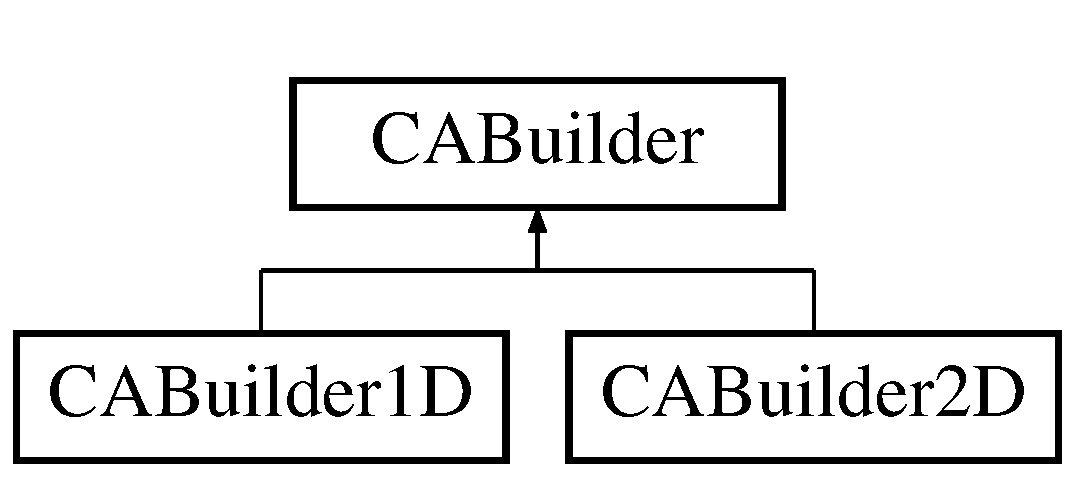
\includegraphics[height=2.000000cm]{class_c_a_builder}
\end{center}
\end{figure}
\subsection*{Fonctions membres publiques}
\begin{DoxyCompactItemize}
\item 
\mbox{\hyperlink{class_voisinage}{Voisinage}} const  $\ast$ \mbox{\hyperlink{class_c_a_builder_a1be1b3d758b2aa2f5798680a8264ca1e}{Get\+Voisinage\+Definition}} () const
\item 
\mbox{\hyperlink{class_transition_rule}{Transition\+Rule}} const  $\ast$ \mbox{\hyperlink{class_c_a_builder_a39da3ad55920be3648c8353f17d12bed}{Get\+Transition\+Rule}} () const
\item 
\mbox{\hyperlink{class_etat}{Etat}} const  $\ast$ \mbox{\hyperlink{class_c_a_builder_a95deea41d8e12b5c5d18cb3c8e24d736}{Get\+Etat\+Depart}} () const
\item 
\mbox{\hyperlink{class_generateur_etat}{Generateur\+Etat}} const  $\ast$ \mbox{\hyperlink{class_c_a_builder_ae304de3db7f44b1192f5a1ae021036a6}{Get\+Generateur\+Etat}} () const
\item 
void \mbox{\hyperlink{class_c_a_builder_a89fe25fa1d52a13756ff47f6b163e7c0}{Build\+Generateur\+Etat\+Random}} ()
\item 
void \mbox{\hyperlink{class_c_a_builder_afbc115fc71d6b17c362e724e5bbcc781}{Build\+Generateur\+Etat\+Symetrie\+Axe\+Vertical}} ()
\end{DoxyCompactItemize}
\subsection*{Fonctions membres protégées}
\begin{DoxyCompactItemize}
\item 
\mbox{\hyperlink{class_c_a_builder_a83d89eba527bee907d22d657fab5fbf6}{C\+A\+Builder}} ()
\item 
virtual \mbox{\hyperlink{class_c_a_builder_a9f917ce136fc4a5d84a89734039f720d}{$\sim$\+C\+A\+Builder}} ()
\item 
\mbox{\hyperlink{class_c_a_builder_af725c741fdb6c5304763638c72d1aa52}{C\+A\+Builder}} (const \mbox{\hyperlink{class_c_a_builder}{C\+A\+Builder}} \&)=delete
\item 
\mbox{\hyperlink{class_c_a_builder}{C\+A\+Builder}} \& \mbox{\hyperlink{class_c_a_builder_a96af5f657cd2b3bebb17c9ce730583a0}{operator=}} (const \mbox{\hyperlink{class_c_a_builder}{C\+A\+Builder}} \&)=delete
\end{DoxyCompactItemize}
\subsection*{Attributs protégés}
\begin{DoxyCompactItemize}
\item 
\mbox{\hyperlink{class_generateur_etat}{Generateur\+Etat}} $\ast$ \mbox{\hyperlink{class_c_a_builder_a8c08002f200d7369f116e2ea1c468ab4}{m\+\_\+generateur\+Etat}}
\item 
\mbox{\hyperlink{class_etat}{Etat}} $\ast$ \mbox{\hyperlink{class_c_a_builder_ac84f3fee62f37c9ae4b78eeff17e6af4}{m\+\_\+etat\+Depart}}
\item 
\mbox{\hyperlink{class_transition_rule}{Transition\+Rule}} $\ast$ \mbox{\hyperlink{class_c_a_builder_af9b64de3a92d0eeef2e7bad30f945ee8}{m\+\_\+transition\+Rule}}
\item 
\mbox{\hyperlink{class_voisinage}{Voisinage}} $\ast$ \mbox{\hyperlink{class_c_a_builder_a8d030d6b0bf0ca88d2bd5b88e1f1b041}{m\+\_\+voisinage\+Definition}}
\end{DoxyCompactItemize}


\subsection{Description détaillée}
Classe de base qui permet de construire les sous-\/parties nécessaire à la construction d\textquotesingle{}un \mbox{\hyperlink{class_cellular_automata}{Cellular\+Automata}}. 

Les constructeurs et destructeurs des classes construitent ne sont pas en private car cette Classe permet juste de stocker les éléments nécessaire à la construction de Cellular\+Automate, ce n\textquotesingle{}est pas une fabrique à proprement parlé et il pourrait être possible de construire ces éléments autrement Par exemple\+: la classe \mbox{\hyperlink{class_cellular_automata}{Cellular\+Automata}} construit des \mbox{\hyperlink{class_etat}{Etat}}. On aurait pu factoriser le code (héritage) des 2 Builder

Cette classe n\textquotesingle{}est pas instanciable car elle ne sert qu\textquotesingle{}à \char`\"{}factoriser\char`\"{} du code commun à \mbox{\hyperlink{class_c_a_builder1_d}{C\+A\+Builder1D}} et \mbox{\hyperlink{class_c_a_builder2_d}{C\+A\+Builder2D}} pour éviter de copier coller le même morceau de code. Mais elle n\textquotesingle{}est pas virtuelle pure (car toutes les méthodes sont bien définies et il est impossible de déclarer une méthode virtuelle pure qui pourra être utile à la fois dans \mbox{\hyperlink{class_c_a_builder1_d}{C\+A\+Builder1D}} et \mbox{\hyperlink{class_c_a_builder2_d}{C\+A\+Builder2D}}

L\textquotesingle{}implémentation necessite de bloquer l\textquotesingle{}utilisation du simulateur lorsqu\textquotesingle{}on fait une modification du simulateur car quand on modifie une sous-\/partie on supprime l\textquotesingle{}ancienne

\begin{DoxyRefDesc}{A faire}
\item[\mbox{\hyperlink{todo__todo000001}{A faire}}]L\textquotesingle{}implémentation ne permet pas de pouvoir éxécuter plusieurs automates cellulaires différents en même temps \end{DoxyRefDesc}


\subsection{Documentation des constructeurs et destructeur}
\mbox{\Hypertarget{class_c_a_builder_a83d89eba527bee907d22d657fab5fbf6}\label{class_c_a_builder_a83d89eba527bee907d22d657fab5fbf6}} 
\index{C\+A\+Builder@{C\+A\+Builder}!C\+A\+Builder@{C\+A\+Builder}}
\index{C\+A\+Builder@{C\+A\+Builder}!C\+A\+Builder@{C\+A\+Builder}}
\subsubsection{\texorpdfstring{C\+A\+Builder()}{CABuilder()}\hspace{0.1cm}{\footnotesize\ttfamily [1/2]}}
{\footnotesize\ttfamily C\+A\+Builder\+::\+C\+A\+Builder (\begin{DoxyParamCaption}{ }\end{DoxyParamCaption})\hspace{0.3cm}{\ttfamily [inline]}, {\ttfamily [protected]}}

\mbox{\Hypertarget{class_c_a_builder_a9f917ce136fc4a5d84a89734039f720d}\label{class_c_a_builder_a9f917ce136fc4a5d84a89734039f720d}} 
\index{C\+A\+Builder@{C\+A\+Builder}!````~C\+A\+Builder@{$\sim$\+C\+A\+Builder}}
\index{````~C\+A\+Builder@{$\sim$\+C\+A\+Builder}!C\+A\+Builder@{C\+A\+Builder}}
\subsubsection{\texorpdfstring{$\sim$\+C\+A\+Builder()}{~CABuilder()}}
{\footnotesize\ttfamily virtual C\+A\+Builder\+::$\sim$\+C\+A\+Builder (\begin{DoxyParamCaption}{ }\end{DoxyParamCaption})\hspace{0.3cm}{\ttfamily [inline]}, {\ttfamily [protected]}, {\ttfamily [virtual]}}

\mbox{\Hypertarget{class_c_a_builder_af725c741fdb6c5304763638c72d1aa52}\label{class_c_a_builder_af725c741fdb6c5304763638c72d1aa52}} 
\index{C\+A\+Builder@{C\+A\+Builder}!C\+A\+Builder@{C\+A\+Builder}}
\index{C\+A\+Builder@{C\+A\+Builder}!C\+A\+Builder@{C\+A\+Builder}}
\subsubsection{\texorpdfstring{C\+A\+Builder()}{CABuilder()}\hspace{0.1cm}{\footnotesize\ttfamily [2/2]}}
{\footnotesize\ttfamily C\+A\+Builder\+::\+C\+A\+Builder (\begin{DoxyParamCaption}\item[{const \mbox{\hyperlink{class_c_a_builder}{C\+A\+Builder}} \&}]{ }\end{DoxyParamCaption})\hspace{0.3cm}{\ttfamily [protected]}, {\ttfamily [delete]}}



\subsection{Documentation des fonctions membres}
\mbox{\Hypertarget{class_c_a_builder_a89fe25fa1d52a13756ff47f6b163e7c0}\label{class_c_a_builder_a89fe25fa1d52a13756ff47f6b163e7c0}} 
\index{C\+A\+Builder@{C\+A\+Builder}!Build\+Generateur\+Etat\+Random@{Build\+Generateur\+Etat\+Random}}
\index{Build\+Generateur\+Etat\+Random@{Build\+Generateur\+Etat\+Random}!C\+A\+Builder@{C\+A\+Builder}}
\subsubsection{\texorpdfstring{Build\+Generateur\+Etat\+Random()}{BuildGenerateurEtatRandom()}}
{\footnotesize\ttfamily void C\+A\+Builder\+::\+Build\+Generateur\+Etat\+Random (\begin{DoxyParamCaption}{ }\end{DoxyParamCaption})\hspace{0.3cm}{\ttfamily [inline]}}

\mbox{\Hypertarget{class_c_a_builder_afbc115fc71d6b17c362e724e5bbcc781}\label{class_c_a_builder_afbc115fc71d6b17c362e724e5bbcc781}} 
\index{C\+A\+Builder@{C\+A\+Builder}!Build\+Generateur\+Etat\+Symetrie\+Axe\+Vertical@{Build\+Generateur\+Etat\+Symetrie\+Axe\+Vertical}}
\index{Build\+Generateur\+Etat\+Symetrie\+Axe\+Vertical@{Build\+Generateur\+Etat\+Symetrie\+Axe\+Vertical}!C\+A\+Builder@{C\+A\+Builder}}
\subsubsection{\texorpdfstring{Build\+Generateur\+Etat\+Symetrie\+Axe\+Vertical()}{BuildGenerateurEtatSymetrieAxeVertical()}}
{\footnotesize\ttfamily void C\+A\+Builder\+::\+Build\+Generateur\+Etat\+Symetrie\+Axe\+Vertical (\begin{DoxyParamCaption}{ }\end{DoxyParamCaption})\hspace{0.3cm}{\ttfamily [inline]}}

\mbox{\Hypertarget{class_c_a_builder_a95deea41d8e12b5c5d18cb3c8e24d736}\label{class_c_a_builder_a95deea41d8e12b5c5d18cb3c8e24d736}} 
\index{C\+A\+Builder@{C\+A\+Builder}!Get\+Etat\+Depart@{Get\+Etat\+Depart}}
\index{Get\+Etat\+Depart@{Get\+Etat\+Depart}!C\+A\+Builder@{C\+A\+Builder}}
\subsubsection{\texorpdfstring{Get\+Etat\+Depart()}{GetEtatDepart()}}
{\footnotesize\ttfamily \mbox{\hyperlink{class_etat}{Etat}} const$\ast$ C\+A\+Builder\+::\+Get\+Etat\+Depart (\begin{DoxyParamCaption}{ }\end{DoxyParamCaption}) const\hspace{0.3cm}{\ttfamily [inline]}}

\mbox{\Hypertarget{class_c_a_builder_ae304de3db7f44b1192f5a1ae021036a6}\label{class_c_a_builder_ae304de3db7f44b1192f5a1ae021036a6}} 
\index{C\+A\+Builder@{C\+A\+Builder}!Get\+Generateur\+Etat@{Get\+Generateur\+Etat}}
\index{Get\+Generateur\+Etat@{Get\+Generateur\+Etat}!C\+A\+Builder@{C\+A\+Builder}}
\subsubsection{\texorpdfstring{Get\+Generateur\+Etat()}{GetGenerateurEtat()}}
{\footnotesize\ttfamily \mbox{\hyperlink{class_generateur_etat}{Generateur\+Etat}} const$\ast$ C\+A\+Builder\+::\+Get\+Generateur\+Etat (\begin{DoxyParamCaption}{ }\end{DoxyParamCaption}) const\hspace{0.3cm}{\ttfamily [inline]}}

\mbox{\Hypertarget{class_c_a_builder_a39da3ad55920be3648c8353f17d12bed}\label{class_c_a_builder_a39da3ad55920be3648c8353f17d12bed}} 
\index{C\+A\+Builder@{C\+A\+Builder}!Get\+Transition\+Rule@{Get\+Transition\+Rule}}
\index{Get\+Transition\+Rule@{Get\+Transition\+Rule}!C\+A\+Builder@{C\+A\+Builder}}
\subsubsection{\texorpdfstring{Get\+Transition\+Rule()}{GetTransitionRule()}}
{\footnotesize\ttfamily \mbox{\hyperlink{class_transition_rule}{Transition\+Rule}} const$\ast$ C\+A\+Builder\+::\+Get\+Transition\+Rule (\begin{DoxyParamCaption}{ }\end{DoxyParamCaption}) const\hspace{0.3cm}{\ttfamily [inline]}}

\mbox{\Hypertarget{class_c_a_builder_a1be1b3d758b2aa2f5798680a8264ca1e}\label{class_c_a_builder_a1be1b3d758b2aa2f5798680a8264ca1e}} 
\index{C\+A\+Builder@{C\+A\+Builder}!Get\+Voisinage\+Definition@{Get\+Voisinage\+Definition}}
\index{Get\+Voisinage\+Definition@{Get\+Voisinage\+Definition}!C\+A\+Builder@{C\+A\+Builder}}
\subsubsection{\texorpdfstring{Get\+Voisinage\+Definition()}{GetVoisinageDefinition()}}
{\footnotesize\ttfamily \mbox{\hyperlink{class_voisinage}{Voisinage}} const$\ast$ C\+A\+Builder\+::\+Get\+Voisinage\+Definition (\begin{DoxyParamCaption}{ }\end{DoxyParamCaption}) const\hspace{0.3cm}{\ttfamily [inline]}}

\mbox{\Hypertarget{class_c_a_builder_a96af5f657cd2b3bebb17c9ce730583a0}\label{class_c_a_builder_a96af5f657cd2b3bebb17c9ce730583a0}} 
\index{C\+A\+Builder@{C\+A\+Builder}!operator=@{operator=}}
\index{operator=@{operator=}!C\+A\+Builder@{C\+A\+Builder}}
\subsubsection{\texorpdfstring{operator=()}{operator=()}}
{\footnotesize\ttfamily \mbox{\hyperlink{class_c_a_builder}{C\+A\+Builder}}\& C\+A\+Builder\+::operator= (\begin{DoxyParamCaption}\item[{const \mbox{\hyperlink{class_c_a_builder}{C\+A\+Builder}} \&}]{ }\end{DoxyParamCaption})\hspace{0.3cm}{\ttfamily [protected]}, {\ttfamily [delete]}}



\subsection{Documentation des données membres}
\mbox{\Hypertarget{class_c_a_builder_ac84f3fee62f37c9ae4b78eeff17e6af4}\label{class_c_a_builder_ac84f3fee62f37c9ae4b78eeff17e6af4}} 
\index{C\+A\+Builder@{C\+A\+Builder}!m\+\_\+etat\+Depart@{m\+\_\+etat\+Depart}}
\index{m\+\_\+etat\+Depart@{m\+\_\+etat\+Depart}!C\+A\+Builder@{C\+A\+Builder}}
\subsubsection{\texorpdfstring{m\+\_\+etat\+Depart}{m\_etatDepart}}
{\footnotesize\ttfamily \mbox{\hyperlink{class_etat}{Etat}}$\ast$ C\+A\+Builder\+::m\+\_\+etat\+Depart\hspace{0.3cm}{\ttfamily [protected]}}

\mbox{\Hypertarget{class_c_a_builder_a8c08002f200d7369f116e2ea1c468ab4}\label{class_c_a_builder_a8c08002f200d7369f116e2ea1c468ab4}} 
\index{C\+A\+Builder@{C\+A\+Builder}!m\+\_\+generateur\+Etat@{m\+\_\+generateur\+Etat}}
\index{m\+\_\+generateur\+Etat@{m\+\_\+generateur\+Etat}!C\+A\+Builder@{C\+A\+Builder}}
\subsubsection{\texorpdfstring{m\+\_\+generateur\+Etat}{m\_generateurEtat}}
{\footnotesize\ttfamily \mbox{\hyperlink{class_generateur_etat}{Generateur\+Etat}}$\ast$ C\+A\+Builder\+::m\+\_\+generateur\+Etat\hspace{0.3cm}{\ttfamily [protected]}}

\mbox{\Hypertarget{class_c_a_builder_af9b64de3a92d0eeef2e7bad30f945ee8}\label{class_c_a_builder_af9b64de3a92d0eeef2e7bad30f945ee8}} 
\index{C\+A\+Builder@{C\+A\+Builder}!m\+\_\+transition\+Rule@{m\+\_\+transition\+Rule}}
\index{m\+\_\+transition\+Rule@{m\+\_\+transition\+Rule}!C\+A\+Builder@{C\+A\+Builder}}
\subsubsection{\texorpdfstring{m\+\_\+transition\+Rule}{m\_transitionRule}}
{\footnotesize\ttfamily \mbox{\hyperlink{class_transition_rule}{Transition\+Rule}}$\ast$ C\+A\+Builder\+::m\+\_\+transition\+Rule\hspace{0.3cm}{\ttfamily [protected]}}

\mbox{\Hypertarget{class_c_a_builder_a8d030d6b0bf0ca88d2bd5b88e1f1b041}\label{class_c_a_builder_a8d030d6b0bf0ca88d2bd5b88e1f1b041}} 
\index{C\+A\+Builder@{C\+A\+Builder}!m\+\_\+voisinage\+Definition@{m\+\_\+voisinage\+Definition}}
\index{m\+\_\+voisinage\+Definition@{m\+\_\+voisinage\+Definition}!C\+A\+Builder@{C\+A\+Builder}}
\subsubsection{\texorpdfstring{m\+\_\+voisinage\+Definition}{m\_voisinageDefinition}}
{\footnotesize\ttfamily \mbox{\hyperlink{class_voisinage}{Voisinage}}$\ast$ C\+A\+Builder\+::m\+\_\+voisinage\+Definition\hspace{0.3cm}{\ttfamily [protected]}}



La documentation de cette classe a été générée à partir du fichier suivant \+:\begin{DoxyCompactItemize}
\item 
C\+:/\+Users/maxn0/git/\+L\+O21/\+Auto\+Cell/\mbox{\hyperlink{cabuilder_8h}{cabuilder.\+h}}\end{DoxyCompactItemize}

\hypertarget{class_c_a_builder1_d}{}\section{Référence de la classe C\+A\+Builder1D}
\label{class_c_a_builder1_d}\index{C\+A\+Builder1D@{C\+A\+Builder1D}}


Classe permettant de construire toutes les sous-\/parties nécessaires à la construction d\textquotesingle{}un automate cellulaire 1D.  




{\ttfamily \#include $<$cabuilder.\+h$>$}

Graphe d\textquotesingle{}héritage de C\+A\+Builder1D\+:\begin{figure}[H]
\begin{center}
\leavevmode
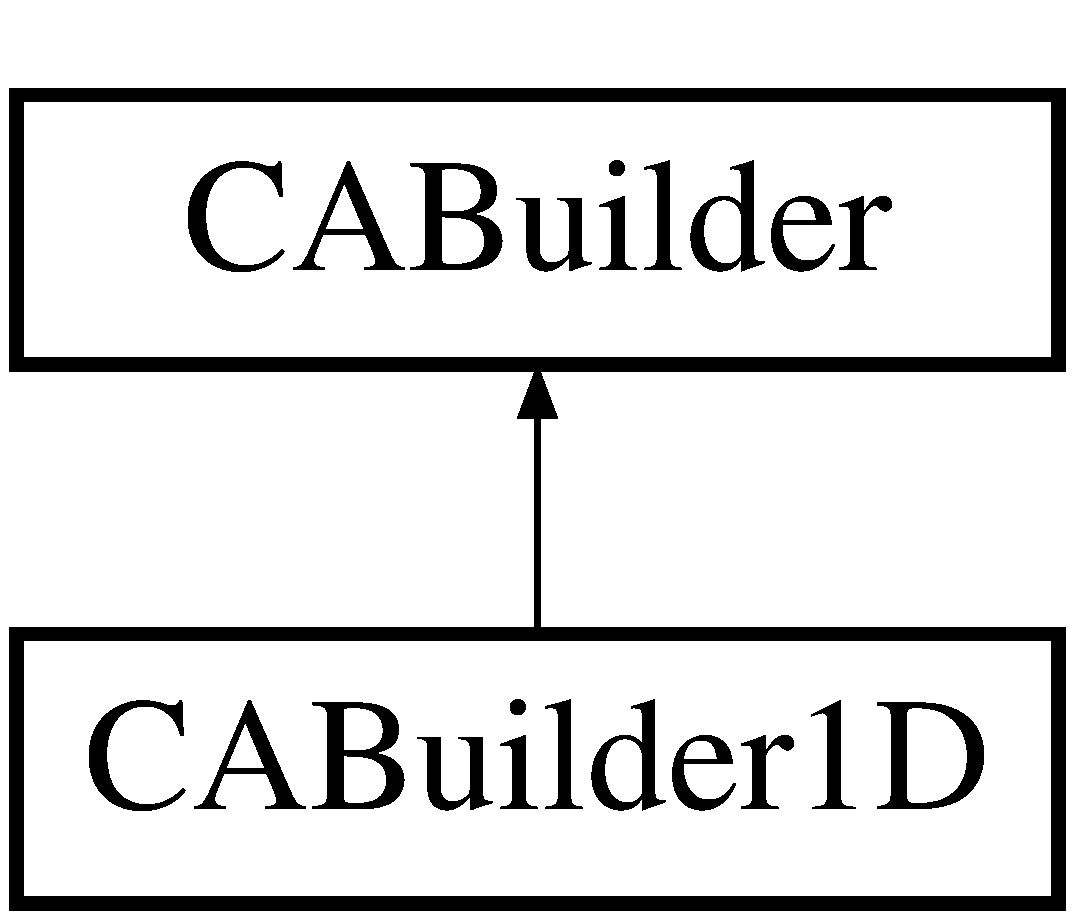
\includegraphics[height=2.000000cm]{class_c_a_builder1_d}
\end{center}
\end{figure}
\subsection*{Fonctions membres publiques}
\begin{DoxyCompactItemize}
\item 
void \mbox{\hyperlink{class_c_a_builder1_d_aa82356e955ae82df3eec34cbb8b47758}{Build\+Voisinage\+Def}} (unsigned int ordre)
\item 
void \mbox{\hyperlink{class_c_a_builder1_d_a8fc01c130a00013416532d7e7b43957a}{Build\+Etat\+Depart}} (unsigned int taille, \mbox{\hyperlink{class_generateur_etat}{Generateur\+Etat}} const \&generateur, int nb\+Etats)
\item 
void \mbox{\hyperlink{class_c_a_builder1_d_a0a274571cddf774bd67fc786dcf1684c}{Build\+Etat\+Depart}} (unsigned int taille, int $\ast$$\ast$tab)
\item 
void \mbox{\hyperlink{class_c_a_builder1_d_a77fa7941654a3c41d68df447b1fd7e5f}{Build\+Etat\+Depart}} (unsigned int taille)
\item 
void \mbox{\hyperlink{class_c_a_builder1_d_a992326d218c98a824f006e6cb03ce011}{Build\+Elementary\+Rule}} (std\+::string const \&rule, unsigned int nb\+Etats)
\end{DoxyCompactItemize}
\subsection*{Fonctions membres publiques statiques}
\begin{DoxyCompactItemize}
\item 
static \mbox{\hyperlink{class_c_a_builder1_d}{C\+A\+Builder1D}} \& \mbox{\hyperlink{class_c_a_builder1_d_a92c5780ec0e58f2d56ee28971a50b134}{get\+Instance}} ()
\end{DoxyCompactItemize}
\subsection*{Fonctions membres privées}
\begin{DoxyCompactItemize}
\item 
\mbox{\hyperlink{class_c_a_builder1_d_a8ce449e2418a22e39cf517baffde61de}{C\+A\+Builder1D}} ()
\item 
\mbox{\hyperlink{class_c_a_builder1_d_a376a4febba2304c52c1ac1c41c8a79a0}{$\sim$\+C\+A\+Builder1D}} ()
\item 
\mbox{\hyperlink{class_c_a_builder1_d_ae0dc5795982306cf2ce982cc2dc2eb22}{C\+A\+Builder1D}} (const \mbox{\hyperlink{class_c_a_builder1_d}{C\+A\+Builder1D}} \&)=delete
\item 
\mbox{\hyperlink{class_c_a_builder1_d}{C\+A\+Builder1D}} \& \mbox{\hyperlink{class_c_a_builder1_d_a3fdf59ff606ba76be957049bc52f79cf}{operator=}} (const \mbox{\hyperlink{class_c_a_builder1_d}{C\+A\+Builder1D}} \&)=delete
\end{DoxyCompactItemize}
\subsection*{Attributs privés}
\begin{DoxyCompactItemize}
\item 
unsigned int \mbox{\hyperlink{class_c_a_builder1_d_a50193db158de49187b1a377fcbff6250}{m\+\_\+nb\+Etats}}
\end{DoxyCompactItemize}
\subsection*{Membres hérités additionnels}


\subsection{Description détaillée}
Classe permettant de construire toutes les sous-\/parties nécessaires à la construction d\textquotesingle{}un automate cellulaire 1D. 

\begin{DoxyRefDesc}{A faire}
\item[\mbox{\hyperlink{todo__todo000002}{A faire}}]L\textquotesingle{}implémentation ne permet pas de pouvoir éxécuter plusieurs automates cellulaires différents en même temps 

améliorer l\textquotesingle{}implémentation pour pouvoir gérer la construction de plusieurs automates en même temps On a décidé de mettre un design pattern singleton sur cette classe afin d\textquotesingle{}être sûr de n\textquotesingle{}avoir qu\textquotesingle{}une seule instance du builder pour créer un seul simulateur 1D car notre application ne peut gérer qu\textquotesingle{}un simulateur 1D à la fois Les constructeurs et destructeurs des classes construitent ne sont pas en private car cette Classe permet juste de stocker les éléments nécessaire à la construction de Cellular\+Automate, ce n\textquotesingle{}est pas une fabrique à proprement parlé et il pourrait être possible de construire ces éléments autrement Par exemple\+: la classe \mbox{\hyperlink{class_cellular_automata}{Cellular\+Automata}} construit des \mbox{\hyperlink{class_etat}{Etat}}. On aurait pu factoriser le code (héritage) des 2 Builder\end{DoxyRefDesc}


C\textquotesingle{}est un singleton car dans notre application il est impossible de gérer plusieurs automates 1D en même temps 

\subsection{Documentation des constructeurs et destructeur}
\mbox{\Hypertarget{class_c_a_builder1_d_a8ce449e2418a22e39cf517baffde61de}\label{class_c_a_builder1_d_a8ce449e2418a22e39cf517baffde61de}} 
\index{C\+A\+Builder1D@{C\+A\+Builder1D}!C\+A\+Builder1D@{C\+A\+Builder1D}}
\index{C\+A\+Builder1D@{C\+A\+Builder1D}!C\+A\+Builder1D@{C\+A\+Builder1D}}
\subsubsection{\texorpdfstring{C\+A\+Builder1\+D()}{CABuilder1D()}\hspace{0.1cm}{\footnotesize\ttfamily [1/2]}}
{\footnotesize\ttfamily C\+A\+Builder1\+D\+::\+C\+A\+Builder1D (\begin{DoxyParamCaption}{ }\end{DoxyParamCaption})\hspace{0.3cm}{\ttfamily [inline]}, {\ttfamily [private]}}

\mbox{\Hypertarget{class_c_a_builder1_d_a376a4febba2304c52c1ac1c41c8a79a0}\label{class_c_a_builder1_d_a376a4febba2304c52c1ac1c41c8a79a0}} 
\index{C\+A\+Builder1D@{C\+A\+Builder1D}!````~C\+A\+Builder1D@{$\sim$\+C\+A\+Builder1D}}
\index{````~C\+A\+Builder1D@{$\sim$\+C\+A\+Builder1D}!C\+A\+Builder1D@{C\+A\+Builder1D}}
\subsubsection{\texorpdfstring{$\sim$\+C\+A\+Builder1\+D()}{~CABuilder1D()}}
{\footnotesize\ttfamily C\+A\+Builder1\+D\+::$\sim$\+C\+A\+Builder1D (\begin{DoxyParamCaption}{ }\end{DoxyParamCaption})\hspace{0.3cm}{\ttfamily [inline]}, {\ttfamily [private]}}

\mbox{\Hypertarget{class_c_a_builder1_d_ae0dc5795982306cf2ce982cc2dc2eb22}\label{class_c_a_builder1_d_ae0dc5795982306cf2ce982cc2dc2eb22}} 
\index{C\+A\+Builder1D@{C\+A\+Builder1D}!C\+A\+Builder1D@{C\+A\+Builder1D}}
\index{C\+A\+Builder1D@{C\+A\+Builder1D}!C\+A\+Builder1D@{C\+A\+Builder1D}}
\subsubsection{\texorpdfstring{C\+A\+Builder1\+D()}{CABuilder1D()}\hspace{0.1cm}{\footnotesize\ttfamily [2/2]}}
{\footnotesize\ttfamily C\+A\+Builder1\+D\+::\+C\+A\+Builder1D (\begin{DoxyParamCaption}\item[{const \mbox{\hyperlink{class_c_a_builder1_d}{C\+A\+Builder1D}} \&}]{ }\end{DoxyParamCaption})\hspace{0.3cm}{\ttfamily [private]}, {\ttfamily [delete]}}



\subsection{Documentation des fonctions membres}
\mbox{\Hypertarget{class_c_a_builder1_d_a992326d218c98a824f006e6cb03ce011}\label{class_c_a_builder1_d_a992326d218c98a824f006e6cb03ce011}} 
\index{C\+A\+Builder1D@{C\+A\+Builder1D}!Build\+Elementary\+Rule@{Build\+Elementary\+Rule}}
\index{Build\+Elementary\+Rule@{Build\+Elementary\+Rule}!C\+A\+Builder1D@{C\+A\+Builder1D}}
\subsubsection{\texorpdfstring{Build\+Elementary\+Rule()}{BuildElementaryRule()}}
{\footnotesize\ttfamily void C\+A\+Builder1\+D\+::\+Build\+Elementary\+Rule (\begin{DoxyParamCaption}\item[{std\+::string const \&}]{rule,  }\item[{unsigned int}]{nb\+Etats }\end{DoxyParamCaption})\hspace{0.3cm}{\ttfamily [inline]}}

\mbox{\Hypertarget{class_c_a_builder1_d_a8fc01c130a00013416532d7e7b43957a}\label{class_c_a_builder1_d_a8fc01c130a00013416532d7e7b43957a}} 
\index{C\+A\+Builder1D@{C\+A\+Builder1D}!Build\+Etat\+Depart@{Build\+Etat\+Depart}}
\index{Build\+Etat\+Depart@{Build\+Etat\+Depart}!C\+A\+Builder1D@{C\+A\+Builder1D}}
\subsubsection{\texorpdfstring{Build\+Etat\+Depart()}{BuildEtatDepart()}\hspace{0.1cm}{\footnotesize\ttfamily [1/3]}}
{\footnotesize\ttfamily void C\+A\+Builder1\+D\+::\+Build\+Etat\+Depart (\begin{DoxyParamCaption}\item[{unsigned int}]{taille,  }\item[{\mbox{\hyperlink{class_generateur_etat}{Generateur\+Etat}} const \&}]{generateur,  }\item[{int}]{nb\+Etats }\end{DoxyParamCaption})\hspace{0.3cm}{\ttfamily [inline]}}

\mbox{\Hypertarget{class_c_a_builder1_d_a0a274571cddf774bd67fc786dcf1684c}\label{class_c_a_builder1_d_a0a274571cddf774bd67fc786dcf1684c}} 
\index{C\+A\+Builder1D@{C\+A\+Builder1D}!Build\+Etat\+Depart@{Build\+Etat\+Depart}}
\index{Build\+Etat\+Depart@{Build\+Etat\+Depart}!C\+A\+Builder1D@{C\+A\+Builder1D}}
\subsubsection{\texorpdfstring{Build\+Etat\+Depart()}{BuildEtatDepart()}\hspace{0.1cm}{\footnotesize\ttfamily [2/3]}}
{\footnotesize\ttfamily void C\+A\+Builder1\+D\+::\+Build\+Etat\+Depart (\begin{DoxyParamCaption}\item[{unsigned int}]{taille,  }\item[{int $\ast$$\ast$}]{tab }\end{DoxyParamCaption})\hspace{0.3cm}{\ttfamily [inline]}}

\mbox{\Hypertarget{class_c_a_builder1_d_a77fa7941654a3c41d68df447b1fd7e5f}\label{class_c_a_builder1_d_a77fa7941654a3c41d68df447b1fd7e5f}} 
\index{C\+A\+Builder1D@{C\+A\+Builder1D}!Build\+Etat\+Depart@{Build\+Etat\+Depart}}
\index{Build\+Etat\+Depart@{Build\+Etat\+Depart}!C\+A\+Builder1D@{C\+A\+Builder1D}}
\subsubsection{\texorpdfstring{Build\+Etat\+Depart()}{BuildEtatDepart()}\hspace{0.1cm}{\footnotesize\ttfamily [3/3]}}
{\footnotesize\ttfamily void C\+A\+Builder1\+D\+::\+Build\+Etat\+Depart (\begin{DoxyParamCaption}\item[{unsigned int}]{taille }\end{DoxyParamCaption})\hspace{0.3cm}{\ttfamily [inline]}}

\mbox{\Hypertarget{class_c_a_builder1_d_aa82356e955ae82df3eec34cbb8b47758}\label{class_c_a_builder1_d_aa82356e955ae82df3eec34cbb8b47758}} 
\index{C\+A\+Builder1D@{C\+A\+Builder1D}!Build\+Voisinage\+Def@{Build\+Voisinage\+Def}}
\index{Build\+Voisinage\+Def@{Build\+Voisinage\+Def}!C\+A\+Builder1D@{C\+A\+Builder1D}}
\subsubsection{\texorpdfstring{Build\+Voisinage\+Def()}{BuildVoisinageDef()}}
{\footnotesize\ttfamily void C\+A\+Builder1\+D\+::\+Build\+Voisinage\+Def (\begin{DoxyParamCaption}\item[{unsigned int}]{ordre }\end{DoxyParamCaption})\hspace{0.3cm}{\ttfamily [inline]}}

\mbox{\Hypertarget{class_c_a_builder1_d_a92c5780ec0e58f2d56ee28971a50b134}\label{class_c_a_builder1_d_a92c5780ec0e58f2d56ee28971a50b134}} 
\index{C\+A\+Builder1D@{C\+A\+Builder1D}!get\+Instance@{get\+Instance}}
\index{get\+Instance@{get\+Instance}!C\+A\+Builder1D@{C\+A\+Builder1D}}
\subsubsection{\texorpdfstring{get\+Instance()}{getInstance()}}
{\footnotesize\ttfamily static \mbox{\hyperlink{class_c_a_builder1_d}{C\+A\+Builder1D}}\& C\+A\+Builder1\+D\+::get\+Instance (\begin{DoxyParamCaption}{ }\end{DoxyParamCaption})\hspace{0.3cm}{\ttfamily [inline]}, {\ttfamily [static]}}

\mbox{\Hypertarget{class_c_a_builder1_d_a3fdf59ff606ba76be957049bc52f79cf}\label{class_c_a_builder1_d_a3fdf59ff606ba76be957049bc52f79cf}} 
\index{C\+A\+Builder1D@{C\+A\+Builder1D}!operator=@{operator=}}
\index{operator=@{operator=}!C\+A\+Builder1D@{C\+A\+Builder1D}}
\subsubsection{\texorpdfstring{operator=()}{operator=()}}
{\footnotesize\ttfamily \mbox{\hyperlink{class_c_a_builder1_d}{C\+A\+Builder1D}}\& C\+A\+Builder1\+D\+::operator= (\begin{DoxyParamCaption}\item[{const \mbox{\hyperlink{class_c_a_builder1_d}{C\+A\+Builder1D}} \&}]{ }\end{DoxyParamCaption})\hspace{0.3cm}{\ttfamily [private]}, {\ttfamily [delete]}}



\subsection{Documentation des données membres}
\mbox{\Hypertarget{class_c_a_builder1_d_a50193db158de49187b1a377fcbff6250}\label{class_c_a_builder1_d_a50193db158de49187b1a377fcbff6250}} 
\index{C\+A\+Builder1D@{C\+A\+Builder1D}!m\+\_\+nb\+Etats@{m\+\_\+nb\+Etats}}
\index{m\+\_\+nb\+Etats@{m\+\_\+nb\+Etats}!C\+A\+Builder1D@{C\+A\+Builder1D}}
\subsubsection{\texorpdfstring{m\+\_\+nb\+Etats}{m\_nbEtats}}
{\footnotesize\ttfamily unsigned int C\+A\+Builder1\+D\+::m\+\_\+nb\+Etats\hspace{0.3cm}{\ttfamily [private]}}



La documentation de cette classe a été générée à partir du fichier suivant \+:\begin{DoxyCompactItemize}
\item 
C\+:/\+Users/maxn0/git/\+L\+O21/\+Auto\+Cell/\mbox{\hyperlink{cabuilder_8h}{cabuilder.\+h}}\end{DoxyCompactItemize}

\hypertarget{class_c_a_builder2_d}{}\section{Référence de la classe C\+A\+Builder2D}
\label{class_c_a_builder2_d}\index{C\+A\+Builder2D@{C\+A\+Builder2D}}


Classe permettant de construire toutes les sous-\/parties nécessaires à la construction d\textquotesingle{}un automate cellulaire 2D.  




{\ttfamily \#include $<$cabuilder.\+h$>$}

Graphe d\textquotesingle{}héritage de C\+A\+Builder2D\+:\begin{figure}[H]
\begin{center}
\leavevmode
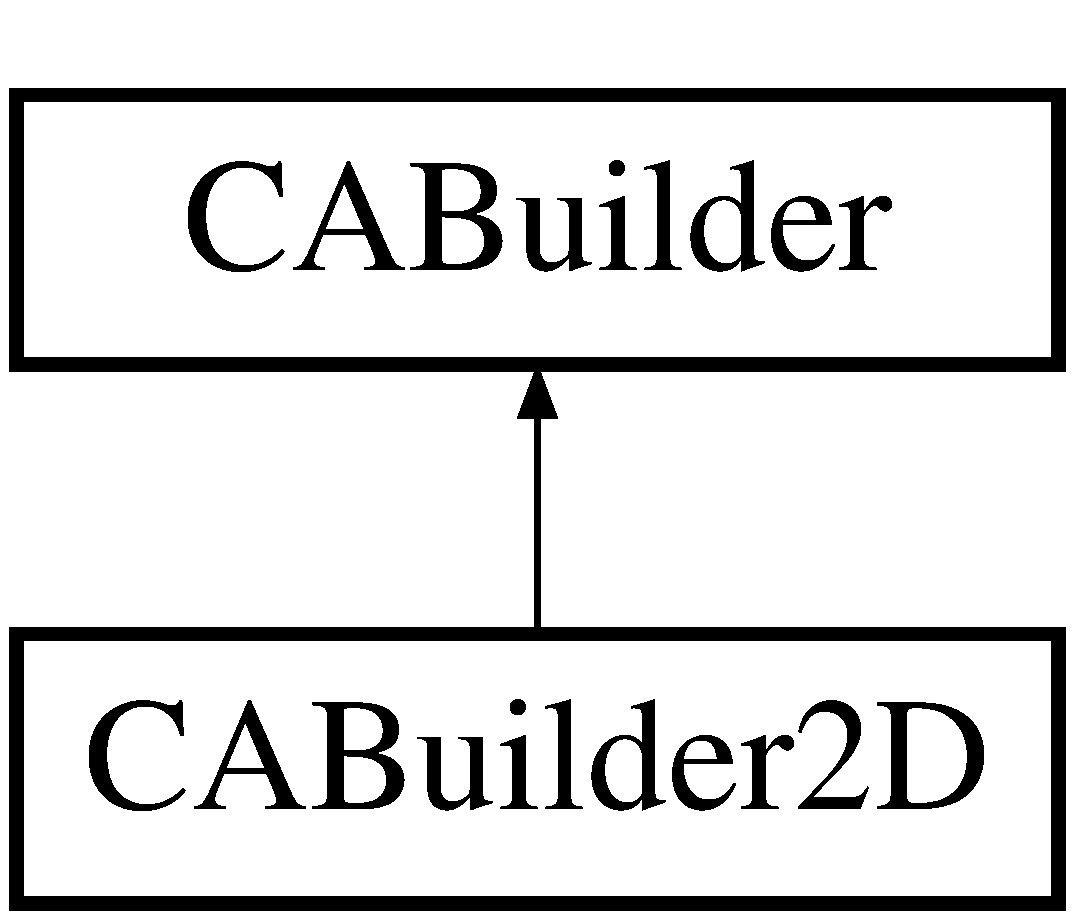
\includegraphics[height=2.000000cm]{class_c_a_builder2_d}
\end{center}
\end{figure}
\subsection*{Fonctions membres publiques}
\begin{DoxyCompactItemize}
\item 
void \mbox{\hyperlink{class_c_a_builder2_d_a0d31f87b74b5058fc60edd47ec372828}{Build\+Voisinage\+Von\+Neumann}} (unsigned int ordre)
\item 
void \mbox{\hyperlink{class_c_a_builder2_d_abafd86f26de9ab72100212edc23fc7fc}{Build\+Voisinage\+Moore}} (unsigned int ordre)
\item 
void \mbox{\hyperlink{class_c_a_builder2_d_af1b276f92d8dd9a914d123b16cc518c7}{Build\+Etat\+Depart}} (unsigned int nb\+Lignes, unsigned int nb\+Colonnes, \mbox{\hyperlink{class_generateur_etat}{Generateur\+Etat}} const \&generateur, int nb\+Etats)
\item 
void \mbox{\hyperlink{class_c_a_builder2_d_aa447c4c66f830ea0dd552592eb606336}{Build\+Etat\+Depart}} (unsigned int nb\+Lignes, unsigned int nb\+Colonnes, int $\ast$$\ast$tab)
\item 
void \mbox{\hyperlink{class_c_a_builder2_d_a7300ec839baa5de1d8c3b9a044b6c3cb}{Build\+Etat\+Depart}} (unsigned int nb\+Lignes, unsigned int nb\+Colonnes)
\item 
void \mbox{\hyperlink{class_c_a_builder2_d_ac8a0719a1a51bfbc40f017808b4c05ed}{Build\+Game\+Of\+Life}} (unsigned int min\+Voisins\+Vivants, unsigned int max\+Voisins\+Vivants)
\item 
void \mbox{\hyperlink{class_c_a_builder2_d_a71f988b3a445b18248661fc4c890a3a0}{Build\+Feu\+Foret}} ()
\end{DoxyCompactItemize}
\subsection*{Fonctions membres publiques statiques}
\begin{DoxyCompactItemize}
\item 
static \mbox{\hyperlink{class_c_a_builder2_d}{C\+A\+Builder2D}} \& \mbox{\hyperlink{class_c_a_builder2_d_a013a50b0ebd4313516febd015db293c2}{get\+Instance}} ()
\end{DoxyCompactItemize}
\subsection*{Fonctions membres privées}
\begin{DoxyCompactItemize}
\item 
\mbox{\hyperlink{class_c_a_builder2_d_a208cc4460b17fb33756e0e384c173760}{C\+A\+Builder2D}} ()
\item 
\mbox{\hyperlink{class_c_a_builder2_d_a8f96127d2894b3a47fd32b8f23d073ba}{$\sim$\+C\+A\+Builder2D}} ()=default
\item 
\mbox{\hyperlink{class_c_a_builder2_d_a55cdd6483a571b716890d73ce4356c91}{C\+A\+Builder2D}} (const \mbox{\hyperlink{class_c_a_builder2_d}{C\+A\+Builder2D}} \&)=delete
\item 
\mbox{\hyperlink{class_c_a_builder2_d}{C\+A\+Builder2D}} \& \mbox{\hyperlink{class_c_a_builder2_d_aa21c22e1d8f10b05bad1b13988adf49d}{operator=}} (const \mbox{\hyperlink{class_c_a_builder2_d}{C\+A\+Builder2D}} \&)=delete
\end{DoxyCompactItemize}
\subsection*{Membres hérités additionnels}


\subsection{Description détaillée}
Classe permettant de construire toutes les sous-\/parties nécessaires à la construction d\textquotesingle{}un automate cellulaire 2D. 

\begin{DoxyRefDesc}{A faire}
\item[\mbox{\hyperlink{todo__todo000003}{A faire}}]L\textquotesingle{}implémentation ne permet pas de pouvoir éxécuter plusieurs automates cellulaires différents en même temps. On 

améliorer l\textquotesingle{}implémentation pour pouvoir gérer la construction de plusieurs automates en même temps Les constructeurs et destructeurs des classes construitent ne sont pas en private car cette Classe permet juste de stocker les éléments nécessaire à la construction de Cellular\+Automate, ce n\textquotesingle{}est pas une fabrique à proprement parlé et il pourrait être possible de construire ces éléments autrement Par exemple\+: la classe \mbox{\hyperlink{class_cellular_automata}{Cellular\+Automata}} construit des \mbox{\hyperlink{class_etat}{Etat}}.\end{DoxyRefDesc}


On a décidé de mettre un design pattern singleton sur cette classe afin d\textquotesingle{}être sûr de n\textquotesingle{}avoir qu\textquotesingle{}une seule instance du builder pour créer un seul simulateur 2D car notre application ne peut gérer qu\textquotesingle{}un simulateur 2D à la fois 

\subsection{Documentation des constructeurs et destructeur}
\mbox{\Hypertarget{class_c_a_builder2_d_a208cc4460b17fb33756e0e384c173760}\label{class_c_a_builder2_d_a208cc4460b17fb33756e0e384c173760}} 
\index{C\+A\+Builder2D@{C\+A\+Builder2D}!C\+A\+Builder2D@{C\+A\+Builder2D}}
\index{C\+A\+Builder2D@{C\+A\+Builder2D}!C\+A\+Builder2D@{C\+A\+Builder2D}}
\subsubsection{\texorpdfstring{C\+A\+Builder2\+D()}{CABuilder2D()}\hspace{0.1cm}{\footnotesize\ttfamily [1/2]}}
{\footnotesize\ttfamily C\+A\+Builder2\+D\+::\+C\+A\+Builder2D (\begin{DoxyParamCaption}{ }\end{DoxyParamCaption})\hspace{0.3cm}{\ttfamily [inline]}, {\ttfamily [private]}}

\mbox{\Hypertarget{class_c_a_builder2_d_a8f96127d2894b3a47fd32b8f23d073ba}\label{class_c_a_builder2_d_a8f96127d2894b3a47fd32b8f23d073ba}} 
\index{C\+A\+Builder2D@{C\+A\+Builder2D}!````~C\+A\+Builder2D@{$\sim$\+C\+A\+Builder2D}}
\index{````~C\+A\+Builder2D@{$\sim$\+C\+A\+Builder2D}!C\+A\+Builder2D@{C\+A\+Builder2D}}
\subsubsection{\texorpdfstring{$\sim$\+C\+A\+Builder2\+D()}{~CABuilder2D()}}
{\footnotesize\ttfamily C\+A\+Builder2\+D\+::$\sim$\+C\+A\+Builder2D (\begin{DoxyParamCaption}{ }\end{DoxyParamCaption})\hspace{0.3cm}{\ttfamily [private]}, {\ttfamily [default]}}

\mbox{\Hypertarget{class_c_a_builder2_d_a55cdd6483a571b716890d73ce4356c91}\label{class_c_a_builder2_d_a55cdd6483a571b716890d73ce4356c91}} 
\index{C\+A\+Builder2D@{C\+A\+Builder2D}!C\+A\+Builder2D@{C\+A\+Builder2D}}
\index{C\+A\+Builder2D@{C\+A\+Builder2D}!C\+A\+Builder2D@{C\+A\+Builder2D}}
\subsubsection{\texorpdfstring{C\+A\+Builder2\+D()}{CABuilder2D()}\hspace{0.1cm}{\footnotesize\ttfamily [2/2]}}
{\footnotesize\ttfamily C\+A\+Builder2\+D\+::\+C\+A\+Builder2D (\begin{DoxyParamCaption}\item[{const \mbox{\hyperlink{class_c_a_builder2_d}{C\+A\+Builder2D}} \&}]{ }\end{DoxyParamCaption})\hspace{0.3cm}{\ttfamily [private]}, {\ttfamily [delete]}}



\subsection{Documentation des fonctions membres}
\mbox{\Hypertarget{class_c_a_builder2_d_af1b276f92d8dd9a914d123b16cc518c7}\label{class_c_a_builder2_d_af1b276f92d8dd9a914d123b16cc518c7}} 
\index{C\+A\+Builder2D@{C\+A\+Builder2D}!Build\+Etat\+Depart@{Build\+Etat\+Depart}}
\index{Build\+Etat\+Depart@{Build\+Etat\+Depart}!C\+A\+Builder2D@{C\+A\+Builder2D}}
\subsubsection{\texorpdfstring{Build\+Etat\+Depart()}{BuildEtatDepart()}\hspace{0.1cm}{\footnotesize\ttfamily [1/3]}}
{\footnotesize\ttfamily void C\+A\+Builder2\+D\+::\+Build\+Etat\+Depart (\begin{DoxyParamCaption}\item[{unsigned int}]{nb\+Lignes,  }\item[{unsigned int}]{nb\+Colonnes,  }\item[{\mbox{\hyperlink{class_generateur_etat}{Generateur\+Etat}} const \&}]{generateur,  }\item[{int}]{nb\+Etats }\end{DoxyParamCaption})\hspace{0.3cm}{\ttfamily [inline]}}

\mbox{\Hypertarget{class_c_a_builder2_d_aa447c4c66f830ea0dd552592eb606336}\label{class_c_a_builder2_d_aa447c4c66f830ea0dd552592eb606336}} 
\index{C\+A\+Builder2D@{C\+A\+Builder2D}!Build\+Etat\+Depart@{Build\+Etat\+Depart}}
\index{Build\+Etat\+Depart@{Build\+Etat\+Depart}!C\+A\+Builder2D@{C\+A\+Builder2D}}
\subsubsection{\texorpdfstring{Build\+Etat\+Depart()}{BuildEtatDepart()}\hspace{0.1cm}{\footnotesize\ttfamily [2/3]}}
{\footnotesize\ttfamily void C\+A\+Builder2\+D\+::\+Build\+Etat\+Depart (\begin{DoxyParamCaption}\item[{unsigned int}]{nb\+Lignes,  }\item[{unsigned int}]{nb\+Colonnes,  }\item[{int $\ast$$\ast$}]{tab }\end{DoxyParamCaption})\hspace{0.3cm}{\ttfamily [inline]}}

\mbox{\Hypertarget{class_c_a_builder2_d_a7300ec839baa5de1d8c3b9a044b6c3cb}\label{class_c_a_builder2_d_a7300ec839baa5de1d8c3b9a044b6c3cb}} 
\index{C\+A\+Builder2D@{C\+A\+Builder2D}!Build\+Etat\+Depart@{Build\+Etat\+Depart}}
\index{Build\+Etat\+Depart@{Build\+Etat\+Depart}!C\+A\+Builder2D@{C\+A\+Builder2D}}
\subsubsection{\texorpdfstring{Build\+Etat\+Depart()}{BuildEtatDepart()}\hspace{0.1cm}{\footnotesize\ttfamily [3/3]}}
{\footnotesize\ttfamily void C\+A\+Builder2\+D\+::\+Build\+Etat\+Depart (\begin{DoxyParamCaption}\item[{unsigned int}]{nb\+Lignes,  }\item[{unsigned int}]{nb\+Colonnes }\end{DoxyParamCaption})\hspace{0.3cm}{\ttfamily [inline]}}

\mbox{\Hypertarget{class_c_a_builder2_d_a71f988b3a445b18248661fc4c890a3a0}\label{class_c_a_builder2_d_a71f988b3a445b18248661fc4c890a3a0}} 
\index{C\+A\+Builder2D@{C\+A\+Builder2D}!Build\+Feu\+Foret@{Build\+Feu\+Foret}}
\index{Build\+Feu\+Foret@{Build\+Feu\+Foret}!C\+A\+Builder2D@{C\+A\+Builder2D}}
\subsubsection{\texorpdfstring{Build\+Feu\+Foret()}{BuildFeuForet()}}
{\footnotesize\ttfamily void C\+A\+Builder2\+D\+::\+Build\+Feu\+Foret (\begin{DoxyParamCaption}{ }\end{DoxyParamCaption})\hspace{0.3cm}{\ttfamily [inline]}}

\mbox{\Hypertarget{class_c_a_builder2_d_ac8a0719a1a51bfbc40f017808b4c05ed}\label{class_c_a_builder2_d_ac8a0719a1a51bfbc40f017808b4c05ed}} 
\index{C\+A\+Builder2D@{C\+A\+Builder2D}!Build\+Game\+Of\+Life@{Build\+Game\+Of\+Life}}
\index{Build\+Game\+Of\+Life@{Build\+Game\+Of\+Life}!C\+A\+Builder2D@{C\+A\+Builder2D}}
\subsubsection{\texorpdfstring{Build\+Game\+Of\+Life()}{BuildGameOfLife()}}
{\footnotesize\ttfamily void C\+A\+Builder2\+D\+::\+Build\+Game\+Of\+Life (\begin{DoxyParamCaption}\item[{unsigned int}]{min\+Voisins\+Vivants,  }\item[{unsigned int}]{max\+Voisins\+Vivants }\end{DoxyParamCaption})\hspace{0.3cm}{\ttfamily [inline]}}

\mbox{\Hypertarget{class_c_a_builder2_d_abafd86f26de9ab72100212edc23fc7fc}\label{class_c_a_builder2_d_abafd86f26de9ab72100212edc23fc7fc}} 
\index{C\+A\+Builder2D@{C\+A\+Builder2D}!Build\+Voisinage\+Moore@{Build\+Voisinage\+Moore}}
\index{Build\+Voisinage\+Moore@{Build\+Voisinage\+Moore}!C\+A\+Builder2D@{C\+A\+Builder2D}}
\subsubsection{\texorpdfstring{Build\+Voisinage\+Moore()}{BuildVoisinageMoore()}}
{\footnotesize\ttfamily void C\+A\+Builder2\+D\+::\+Build\+Voisinage\+Moore (\begin{DoxyParamCaption}\item[{unsigned int}]{ordre }\end{DoxyParamCaption})\hspace{0.3cm}{\ttfamily [inline]}}

\mbox{\Hypertarget{class_c_a_builder2_d_a0d31f87b74b5058fc60edd47ec372828}\label{class_c_a_builder2_d_a0d31f87b74b5058fc60edd47ec372828}} 
\index{C\+A\+Builder2D@{C\+A\+Builder2D}!Build\+Voisinage\+Von\+Neumann@{Build\+Voisinage\+Von\+Neumann}}
\index{Build\+Voisinage\+Von\+Neumann@{Build\+Voisinage\+Von\+Neumann}!C\+A\+Builder2D@{C\+A\+Builder2D}}
\subsubsection{\texorpdfstring{Build\+Voisinage\+Von\+Neumann()}{BuildVoisinageVonNeumann()}}
{\footnotesize\ttfamily void C\+A\+Builder2\+D\+::\+Build\+Voisinage\+Von\+Neumann (\begin{DoxyParamCaption}\item[{unsigned int}]{ordre }\end{DoxyParamCaption})\hspace{0.3cm}{\ttfamily [inline]}}

\mbox{\Hypertarget{class_c_a_builder2_d_a013a50b0ebd4313516febd015db293c2}\label{class_c_a_builder2_d_a013a50b0ebd4313516febd015db293c2}} 
\index{C\+A\+Builder2D@{C\+A\+Builder2D}!get\+Instance@{get\+Instance}}
\index{get\+Instance@{get\+Instance}!C\+A\+Builder2D@{C\+A\+Builder2D}}
\subsubsection{\texorpdfstring{get\+Instance()}{getInstance()}}
{\footnotesize\ttfamily static \mbox{\hyperlink{class_c_a_builder2_d}{C\+A\+Builder2D}}\& C\+A\+Builder2\+D\+::get\+Instance (\begin{DoxyParamCaption}{ }\end{DoxyParamCaption})\hspace{0.3cm}{\ttfamily [inline]}, {\ttfamily [static]}}

\mbox{\Hypertarget{class_c_a_builder2_d_aa21c22e1d8f10b05bad1b13988adf49d}\label{class_c_a_builder2_d_aa21c22e1d8f10b05bad1b13988adf49d}} 
\index{C\+A\+Builder2D@{C\+A\+Builder2D}!operator=@{operator=}}
\index{operator=@{operator=}!C\+A\+Builder2D@{C\+A\+Builder2D}}
\subsubsection{\texorpdfstring{operator=()}{operator=()}}
{\footnotesize\ttfamily \mbox{\hyperlink{class_c_a_builder2_d}{C\+A\+Builder2D}}\& C\+A\+Builder2\+D\+::operator= (\begin{DoxyParamCaption}\item[{const \mbox{\hyperlink{class_c_a_builder2_d}{C\+A\+Builder2D}} \&}]{ }\end{DoxyParamCaption})\hspace{0.3cm}{\ttfamily [private]}, {\ttfamily [delete]}}



La documentation de cette classe a été générée à partir du fichier suivant \+:\begin{DoxyCompactItemize}
\item 
C\+:/\+Users/maxn0/git/\+L\+O21/\+Auto\+Cell/\mbox{\hyperlink{cabuilder_8h}{cabuilder.\+h}}\end{DoxyCompactItemize}

\hypertarget{class_cell}{}\section{Référence de la classe Cell}
\label{class_cell}\index{Cell@{Cell}}


classe représentant une cellule \+: élément de base du programme  




{\ttfamily \#include $<$cell.\+h$>$}

\subsection*{Fonctions membres publiques}
\begin{DoxyCompactItemize}
\item 
std\+::vector$<$ \mbox{\hyperlink{class_cell}{Cell}} $\ast$ $>$ const  \& \mbox{\hyperlink{class_cell_a5c2a7b09dcb8afed0040ebdc4267408d}{Get\+Voisins}} () const
\begin{DoxyCompactList}\small\item\em Accesseur en lecture sur m\+\_\+voisins. \end{DoxyCompactList}\item 
int \mbox{\hyperlink{class_cell_a7640093c787979958fbb772e4fccdffa}{Get\+Etat}} () const
\begin{DoxyCompactList}\small\item\em Accesseur en lecture sur m\+\_\+etat. \end{DoxyCompactList}\item 
int \mbox{\hyperlink{class_cell_a3af5ea9b9e031151e16009b22118b07a}{GetX}} () const
\begin{DoxyCompactList}\small\item\em Accesseur en lecture sur m\+\_\+x. \end{DoxyCompactList}\item 
int \mbox{\hyperlink{class_cell_a3668c9664cadb1b94a632d497fa493c5}{GetY}} () const
\begin{DoxyCompactList}\small\item\em Accesseur en lecture sur m\+\_\+y. \end{DoxyCompactList}\item 
void \mbox{\hyperlink{class_cell_a33dac87ec7294fdb4c67b8b430ea0946}{Set\+Etat}} (int \mbox{\hyperlink{cell_8h_ae60adcb558b7f2142c3aa2dd94aaa535}{etat}})
\begin{DoxyCompactList}\small\item\em modification de l\textquotesingle{}etat \end{DoxyCompactList}\item 
void \mbox{\hyperlink{class_cell_aef5912d85e2ca3e034023fb0874896fa}{Ajouter\+Voisin}} (\mbox{\hyperlink{class_cell}{Cell}} $\ast$voisin)
\begin{DoxyCompactList}\small\item\em ajout d\textquotesingle{}un voisin dans le voisinage de la cellule \end{DoxyCompactList}\item 
void \mbox{\hyperlink{class_cell_a4f07be87bb04bdc457726c51f2c69bcc}{Clear\+Voisinage}} ()
\begin{DoxyCompactList}\small\item\em Suppression du voisinage. \end{DoxyCompactList}\end{DoxyCompactItemize}
\subsection*{Fonctions membres privées}
\begin{DoxyCompactItemize}
\item 
\mbox{\hyperlink{class_cell_a508f988fb5b1ef8358589363c1af3ee4}{$\sim$\+Cell}} ()=default
\begin{DoxyCompactList}\small\item\em Destructeur par défaut. \end{DoxyCompactList}\item 
\mbox{\hyperlink{class_cell_a394510643e8664cf12b5efaf5cb99f71}{Cell}} ()
\begin{DoxyCompactList}\small\item\em Constructeur. \end{DoxyCompactList}\item 
\mbox{\hyperlink{class_cell_abfff4b378d15d85506663df528762eaf}{Cell}} (int \mbox{\hyperlink{cell_8h_ae60adcb558b7f2142c3aa2dd94aaa535}{etat}}, int x, int y)
\begin{DoxyCompactList}\small\item\em Constructeur. \end{DoxyCompactList}\item 
\mbox{\hyperlink{class_cell_aff4c807938a63e9469c1547e7c087e0b}{Cell}} (\mbox{\hyperlink{class_cell}{Cell}} const \&c)=default
\begin{DoxyCompactList}\small\item\em Constructeur de recopie. \end{DoxyCompactList}\item 
void \mbox{\hyperlink{class_cell_a9aaedcce2daccb4aa070f870c1a207ed}{SetX}} (int x)
\begin{DoxyCompactList}\small\item\em modification de la position X \end{DoxyCompactList}\item 
void \mbox{\hyperlink{class_cell_a48afb0c8c8d1ebe3409b9a166dcd507d}{SetY}} (int y)
\begin{DoxyCompactList}\small\item\em modification de la position Y \end{DoxyCompactList}\item 
\mbox{\hyperlink{class_cell}{Cell}} \& \mbox{\hyperlink{class_cell_ac1f905d4cd626cc32963ab7a6f76634e}{operator=}} (\mbox{\hyperlink{class_cell}{Cell}} const \&c)=default
\begin{DoxyCompactList}\small\item\em surcharge de l\textquotesingle{}opérateur d\textquotesingle{}affectation (défaut) \end{DoxyCompactList}\end{DoxyCompactItemize}
\subsection*{Attributs privés}
\begin{DoxyCompactItemize}
\item 
int \mbox{\hyperlink{class_cell_a350cfee41db7450651de4e48543227c3}{m\+\_\+etat}}
\begin{DoxyCompactList}\small\item\em état (valeur) de la cellule. \end{DoxyCompactList}\item 
std\+::vector$<$ \mbox{\hyperlink{class_cell}{Cell}} $\ast$ $>$ \mbox{\hyperlink{class_cell_a7d781cbf0f2a5dffd13313b8eab86732}{m\+\_\+voisins}}
\begin{DoxyCompactList}\small\item\em vecteur de pointeurs sur les cellules voisines de la cellule \end{DoxyCompactList}\item 
int \mbox{\hyperlink{class_cell_ae38c546e6fd703965c8b62f750e68417}{m\+\_\+x}}
\begin{DoxyCompactList}\small\item\em position en ligne de la cellule \end{DoxyCompactList}\item 
int \mbox{\hyperlink{class_cell_a303c301e529e95ce1eadaf5b73ad41b2}{m\+\_\+y}}
\begin{DoxyCompactList}\small\item\em position en colonne de la cellule \end{DoxyCompactList}\end{DoxyCompactItemize}
\subsection*{Amis}
\begin{DoxyCompactItemize}
\item 
class \mbox{\hyperlink{class_cell_af495e82aa15594b628d4192e8ecb688b}{Etat}}
\end{DoxyCompactItemize}


\subsection{Description détaillée}
classe représentant une cellule \+: élément de base du programme 

Un objet \mbox{\hyperlink{class_cell}{Cell}} est une cellule qui fait nécessairement partie d\textquotesingle{}un objet \mbox{\hyperlink{class_etat}{Etat}} car seule \mbox{\hyperlink{class_etat}{Etat}} peut construire des objets \mbox{\hyperlink{class_cell}{Cell}}. Une cellule est caractérisée par sa position, son état (sa valeur), un voisinage. 

\subsection{Documentation des constructeurs et destructeur}
\mbox{\Hypertarget{class_cell_a508f988fb5b1ef8358589363c1af3ee4}\label{class_cell_a508f988fb5b1ef8358589363c1af3ee4}} 
\index{Cell@{Cell}!````~Cell@{$\sim$\+Cell}}
\index{````~Cell@{$\sim$\+Cell}!Cell@{Cell}}
\subsubsection{\texorpdfstring{$\sim$\+Cell()}{~Cell()}}
{\footnotesize\ttfamily Cell\+::$\sim$\+Cell (\begin{DoxyParamCaption}{ }\end{DoxyParamCaption})\hspace{0.3cm}{\ttfamily [private]}, {\ttfamily [default]}}



Destructeur par défaut. 

\mbox{\Hypertarget{class_cell_a394510643e8664cf12b5efaf5cb99f71}\label{class_cell_a394510643e8664cf12b5efaf5cb99f71}} 
\index{Cell@{Cell}!Cell@{Cell}}
\index{Cell@{Cell}!Cell@{Cell}}
\subsubsection{\texorpdfstring{Cell()}{Cell()}\hspace{0.1cm}{\footnotesize\ttfamily [1/3]}}
{\footnotesize\ttfamily Cell\+::\+Cell (\begin{DoxyParamCaption}{ }\end{DoxyParamCaption})\hspace{0.3cm}{\ttfamily [inline]}, {\ttfamily [private]}}



Constructeur. 

Constructeur par défault de la classe \mbox{\hyperlink{class_cell}{Cell}} \+: X, Y et l\textquotesingle{}état sont initialisés à 0. Seule la classe \mbox{\hyperlink{class_etat}{Etat}} peut construire des \mbox{\hyperlink{class_cell}{Cell}}. \mbox{\Hypertarget{class_cell_abfff4b378d15d85506663df528762eaf}\label{class_cell_abfff4b378d15d85506663df528762eaf}} 
\index{Cell@{Cell}!Cell@{Cell}}
\index{Cell@{Cell}!Cell@{Cell}}
\subsubsection{\texorpdfstring{Cell()}{Cell()}\hspace{0.1cm}{\footnotesize\ttfamily [2/3]}}
{\footnotesize\ttfamily Cell\+::\+Cell (\begin{DoxyParamCaption}\item[{int}]{etat,  }\item[{int}]{x,  }\item[{int}]{y }\end{DoxyParamCaption})\hspace{0.3cm}{\ttfamily [inline]}, {\ttfamily [private]}}



Constructeur. 

Constructeur de la classe \mbox{\hyperlink{class_cell}{Cell}}. Seule la classe \mbox{\hyperlink{class_etat}{Etat}} peut construire des \mbox{\hyperlink{class_cell}{Cell}}.


\begin{DoxyParams}{Paramètres}
{\em etat} & \+: valeur prise par la cellule \\
\hline
{\em x,y} & \+: positions \\
\hline
\end{DoxyParams}
\mbox{\Hypertarget{class_cell_aff4c807938a63e9469c1547e7c087e0b}\label{class_cell_aff4c807938a63e9469c1547e7c087e0b}} 
\index{Cell@{Cell}!Cell@{Cell}}
\index{Cell@{Cell}!Cell@{Cell}}
\subsubsection{\texorpdfstring{Cell()}{Cell()}\hspace{0.1cm}{\footnotesize\ttfamily [3/3]}}
{\footnotesize\ttfamily Cell\+::\+Cell (\begin{DoxyParamCaption}\item[{\mbox{\hyperlink{class_cell}{Cell}} const \&}]{c }\end{DoxyParamCaption})\hspace{0.3cm}{\ttfamily [private]}, {\ttfamily [default]}}



Constructeur de recopie. 

Constructeur de recopie de la classe \mbox{\hyperlink{class_cell}{Cell}}. Seule la classe \mbox{\hyperlink{class_etat}{Etat}} peut construire des \mbox{\hyperlink{class_cell}{Cell}}. 
\begin{DoxyParams}{Paramètres}
{\em c} & \+: référence sur la \mbox{\hyperlink{class_cell}{Cell}} qu\textquotesingle{}on souhaite copier \\
\hline
\end{DoxyParams}


\subsection{Documentation des fonctions membres}
\mbox{\Hypertarget{class_cell_aef5912d85e2ca3e034023fb0874896fa}\label{class_cell_aef5912d85e2ca3e034023fb0874896fa}} 
\index{Cell@{Cell}!Ajouter\+Voisin@{Ajouter\+Voisin}}
\index{Ajouter\+Voisin@{Ajouter\+Voisin}!Cell@{Cell}}
\subsubsection{\texorpdfstring{Ajouter\+Voisin()}{AjouterVoisin()}}
{\footnotesize\ttfamily void Cell\+::\+Ajouter\+Voisin (\begin{DoxyParamCaption}\item[{\mbox{\hyperlink{class_cell}{Cell}} $\ast$}]{voisin }\end{DoxyParamCaption})}



ajout d\textquotesingle{}un voisin dans le voisinage de la cellule 


\begin{DoxyParams}{Paramètres}
{\em voisin} & = pointeur sur la cellule voisine à ajouter \\
\hline
\end{DoxyParams}
\mbox{\Hypertarget{class_cell_a4f07be87bb04bdc457726c51f2c69bcc}\label{class_cell_a4f07be87bb04bdc457726c51f2c69bcc}} 
\index{Cell@{Cell}!Clear\+Voisinage@{Clear\+Voisinage}}
\index{Clear\+Voisinage@{Clear\+Voisinage}!Cell@{Cell}}
\subsubsection{\texorpdfstring{Clear\+Voisinage()}{ClearVoisinage()}}
{\footnotesize\ttfamily void Cell\+::\+Clear\+Voisinage (\begin{DoxyParamCaption}{ }\end{DoxyParamCaption})\hspace{0.3cm}{\ttfamily [inline]}}



Suppression du voisinage. 

\mbox{\Hypertarget{class_cell_a7640093c787979958fbb772e4fccdffa}\label{class_cell_a7640093c787979958fbb772e4fccdffa}} 
\index{Cell@{Cell}!Get\+Etat@{Get\+Etat}}
\index{Get\+Etat@{Get\+Etat}!Cell@{Cell}}
\subsubsection{\texorpdfstring{Get\+Etat()}{GetEtat()}}
{\footnotesize\ttfamily int Cell\+::\+Get\+Etat (\begin{DoxyParamCaption}{ }\end{DoxyParamCaption}) const\hspace{0.3cm}{\ttfamily [inline]}}



Accesseur en lecture sur m\+\_\+etat. 

\begin{DoxyReturn}{Renvoie}
etat de la cellule 
\end{DoxyReturn}
\mbox{\Hypertarget{class_cell_a5c2a7b09dcb8afed0040ebdc4267408d}\label{class_cell_a5c2a7b09dcb8afed0040ebdc4267408d}} 
\index{Cell@{Cell}!Get\+Voisins@{Get\+Voisins}}
\index{Get\+Voisins@{Get\+Voisins}!Cell@{Cell}}
\subsubsection{\texorpdfstring{Get\+Voisins()}{GetVoisins()}}
{\footnotesize\ttfamily std\+::vector$<$\mbox{\hyperlink{class_cell}{Cell}}$\ast$$>$ const\& Cell\+::\+Get\+Voisins (\begin{DoxyParamCaption}{ }\end{DoxyParamCaption}) const\hspace{0.3cm}{\ttfamily [inline]}}



Accesseur en lecture sur m\+\_\+voisins. 

Méthode permettant de récupérer une référence const sur l\textquotesingle{}ensemble des voisins d\textquotesingle{}une cellule. \begin{DoxyReturn}{Renvoie}
référence const sur le voisinage de la cellule qui est un vector de pointeurs de type \mbox{\hyperlink{class_cell}{Cell}} pointant chacun sur une cellule voisine de la cellule. 
\end{DoxyReturn}
\mbox{\Hypertarget{class_cell_a3af5ea9b9e031151e16009b22118b07a}\label{class_cell_a3af5ea9b9e031151e16009b22118b07a}} 
\index{Cell@{Cell}!GetX@{GetX}}
\index{GetX@{GetX}!Cell@{Cell}}
\subsubsection{\texorpdfstring{Get\+X()}{GetX()}}
{\footnotesize\ttfamily int Cell\+::\+GetX (\begin{DoxyParamCaption}{ }\end{DoxyParamCaption}) const\hspace{0.3cm}{\ttfamily [inline]}}



Accesseur en lecture sur m\+\_\+x. 

\begin{DoxyReturn}{Renvoie}
position en X (ligne) 
\end{DoxyReturn}
\mbox{\Hypertarget{class_cell_a3668c9664cadb1b94a632d497fa493c5}\label{class_cell_a3668c9664cadb1b94a632d497fa493c5}} 
\index{Cell@{Cell}!GetY@{GetY}}
\index{GetY@{GetY}!Cell@{Cell}}
\subsubsection{\texorpdfstring{Get\+Y()}{GetY()}}
{\footnotesize\ttfamily int Cell\+::\+GetY (\begin{DoxyParamCaption}{ }\end{DoxyParamCaption}) const\hspace{0.3cm}{\ttfamily [inline]}}



Accesseur en lecture sur m\+\_\+y. 

\begin{DoxyReturn}{Renvoie}
position en Y (colonne) 
\end{DoxyReturn}
\mbox{\Hypertarget{class_cell_ac1f905d4cd626cc32963ab7a6f76634e}\label{class_cell_ac1f905d4cd626cc32963ab7a6f76634e}} 
\index{Cell@{Cell}!operator=@{operator=}}
\index{operator=@{operator=}!Cell@{Cell}}
\subsubsection{\texorpdfstring{operator=()}{operator=()}}
{\footnotesize\ttfamily \mbox{\hyperlink{class_cell}{Cell}}\& Cell\+::operator= (\begin{DoxyParamCaption}\item[{\mbox{\hyperlink{class_cell}{Cell}} const \&}]{c }\end{DoxyParamCaption})\hspace{0.3cm}{\ttfamily [private]}, {\ttfamily [default]}}



surcharge de l\textquotesingle{}opérateur d\textquotesingle{}affectation (défaut) 


\begin{DoxyParams}{Paramètres}
{\em c} & \+: référence sur la cellule qui va nous servir à affecter la cellule courante \\
\hline
\end{DoxyParams}
\mbox{\Hypertarget{class_cell_a33dac87ec7294fdb4c67b8b430ea0946}\label{class_cell_a33dac87ec7294fdb4c67b8b430ea0946}} 
\index{Cell@{Cell}!Set\+Etat@{Set\+Etat}}
\index{Set\+Etat@{Set\+Etat}!Cell@{Cell}}
\subsubsection{\texorpdfstring{Set\+Etat()}{SetEtat()}}
{\footnotesize\ttfamily void Cell\+::\+Set\+Etat (\begin{DoxyParamCaption}\item[{int}]{etat }\end{DoxyParamCaption})}



modification de l\textquotesingle{}etat 


\begin{DoxyParams}{Paramètres}
{\em etat} & \+: valeur prise par la cellule \\
\hline
\end{DoxyParams}
\mbox{\Hypertarget{class_cell_a9aaedcce2daccb4aa070f870c1a207ed}\label{class_cell_a9aaedcce2daccb4aa070f870c1a207ed}} 
\index{Cell@{Cell}!SetX@{SetX}}
\index{SetX@{SetX}!Cell@{Cell}}
\subsubsection{\texorpdfstring{Set\+X()}{SetX()}}
{\footnotesize\ttfamily void Cell\+::\+SetX (\begin{DoxyParamCaption}\item[{int}]{x }\end{DoxyParamCaption})\hspace{0.3cm}{\ttfamily [private]}}



modification de la position X 

accesseur en écriture sur m\+\_\+x. Seule la classe \mbox{\hyperlink{class_etat}{Etat}} peut l\textquotesingle{}utiliser car il est illogique d\textquotesingle{}affecter une position X en dehors d\textquotesingle{}une grille. (Cet accesseur n\textquotesingle{}a pas grand intérêt car la classe \mbox{\hyperlink{class_etat}{Etat}} pourrait modifier m\+\_\+x directement vu que c\textquotesingle{}est une classe amie, mais nous avons pris la décision d\textquotesingle{}en faire une classe amie plus tard donc nous l\textquotesingle{}avons laissé afin de ne pas remodifier le code de la classe \mbox{\hyperlink{class_etat}{Etat}}) 
\begin{DoxyParams}{Paramètres}
{\em x} & \+: ligne \\
\hline
\end{DoxyParams}
\mbox{\Hypertarget{class_cell_a48afb0c8c8d1ebe3409b9a166dcd507d}\label{class_cell_a48afb0c8c8d1ebe3409b9a166dcd507d}} 
\index{Cell@{Cell}!SetY@{SetY}}
\index{SetY@{SetY}!Cell@{Cell}}
\subsubsection{\texorpdfstring{Set\+Y()}{SetY()}}
{\footnotesize\ttfamily void Cell\+::\+SetY (\begin{DoxyParamCaption}\item[{int}]{y }\end{DoxyParamCaption})\hspace{0.3cm}{\ttfamily [private]}}



modification de la position Y 

accesseur en écriture sur m\+\_\+y. Seule la classe \mbox{\hyperlink{class_etat}{Etat}} peut l\textquotesingle{}utiliser car il est illogique d\textquotesingle{}affecter une position Y en dehors d\textquotesingle{}une grille. (Cet accesseur n\textquotesingle{}a pas grand intérêt car la classe \mbox{\hyperlink{class_etat}{Etat}} pourrait modifier m\+\_\+y directement vu que c\textquotesingle{}est une classe amie, mais nous avons pris la décision d\textquotesingle{}en faire une classe amie plus tard donc nous l\textquotesingle{}avons laissé afin de ne pas remodifier le code de la classe \mbox{\hyperlink{class_etat}{Etat}}) 
\begin{DoxyParams}{Paramètres}
{\em y} & \+: colonne \\
\hline
\end{DoxyParams}


\subsection{Documentation des fonctions amies et associées}
\mbox{\Hypertarget{class_cell_af495e82aa15594b628d4192e8ecb688b}\label{class_cell_af495e82aa15594b628d4192e8ecb688b}} 
\index{Cell@{Cell}!Etat@{Etat}}
\index{Etat@{Etat}!Cell@{Cell}}
\subsubsection{\texorpdfstring{Etat}{Etat}}
{\footnotesize\ttfamily friend class \mbox{\hyperlink{class_etat}{Etat}}\hspace{0.3cm}{\ttfamily [friend]}}



\subsection{Documentation des données membres}
\mbox{\Hypertarget{class_cell_a350cfee41db7450651de4e48543227c3}\label{class_cell_a350cfee41db7450651de4e48543227c3}} 
\index{Cell@{Cell}!m\+\_\+etat@{m\+\_\+etat}}
\index{m\+\_\+etat@{m\+\_\+etat}!Cell@{Cell}}
\subsubsection{\texorpdfstring{m\+\_\+etat}{m\_etat}}
{\footnotesize\ttfamily int Cell\+::m\+\_\+etat\hspace{0.3cm}{\ttfamily [private]}}



état (valeur) de la cellule. 

\mbox{\Hypertarget{class_cell_a7d781cbf0f2a5dffd13313b8eab86732}\label{class_cell_a7d781cbf0f2a5dffd13313b8eab86732}} 
\index{Cell@{Cell}!m\+\_\+voisins@{m\+\_\+voisins}}
\index{m\+\_\+voisins@{m\+\_\+voisins}!Cell@{Cell}}
\subsubsection{\texorpdfstring{m\+\_\+voisins}{m\_voisins}}
{\footnotesize\ttfamily std\+::vector$<$\mbox{\hyperlink{class_cell}{Cell}}$\ast$$>$ Cell\+::m\+\_\+voisins\hspace{0.3cm}{\ttfamily [private]}}



vecteur de pointeurs sur les cellules voisines de la cellule 

\mbox{\Hypertarget{class_cell_ae38c546e6fd703965c8b62f750e68417}\label{class_cell_ae38c546e6fd703965c8b62f750e68417}} 
\index{Cell@{Cell}!m\+\_\+x@{m\+\_\+x}}
\index{m\+\_\+x@{m\+\_\+x}!Cell@{Cell}}
\subsubsection{\texorpdfstring{m\+\_\+x}{m\_x}}
{\footnotesize\ttfamily int Cell\+::m\+\_\+x\hspace{0.3cm}{\ttfamily [private]}}



position en ligne de la cellule 

\mbox{\Hypertarget{class_cell_a303c301e529e95ce1eadaf5b73ad41b2}\label{class_cell_a303c301e529e95ce1eadaf5b73ad41b2}} 
\index{Cell@{Cell}!m\+\_\+y@{m\+\_\+y}}
\index{m\+\_\+y@{m\+\_\+y}!Cell@{Cell}}
\subsubsection{\texorpdfstring{m\+\_\+y}{m\_y}}
{\footnotesize\ttfamily int Cell\+::m\+\_\+y\hspace{0.3cm}{\ttfamily [private]}}



position en colonne de la cellule 



La documentation de cette classe a été générée à partir des fichiers suivants \+:\begin{DoxyCompactItemize}
\item 
C\+:/\+Users/maxn0/git/\+L\+O21/\+Auto\+Cell/\mbox{\hyperlink{cell_8h}{cell.\+h}}\item 
C\+:/\+Users/maxn0/git/\+L\+O21/\+Auto\+Cell/\mbox{\hyperlink{cell_8cpp}{cell.\+cpp}}\end{DoxyCompactItemize}

\hypertarget{class_cellular_automata}{}\section{Référence de la classe Cellular\+Automata}
\label{class_cellular_automata}\index{Cellular\+Automata@{Cellular\+Automata}}


{\ttfamily \#include $<$cellularautomata.\+h$>$}

\subsection*{Fonctions membres publiques}
\begin{DoxyCompactItemize}
\item 
\mbox{\hyperlink{class_cellular_automata_af50a5ecce37ce634058c6cd8724f6732}{Cellular\+Automata}} (unsigned int nb\+Etats, const \mbox{\hyperlink{class_etat}{Etat}} $\ast$dep=nullptr, const \mbox{\hyperlink{class_transition_rule}{Transition\+Rule}} $\ast$rule=nullptr, const \mbox{\hyperlink{class_voisinage}{Voisinage}} $\ast$definition\+Voisinage=nullptr, unsigned int buffer=2)
\item 
void \mbox{\hyperlink{class_cellular_automata_a8ee6a9ee70fccd7987805e3d176fb3e1}{set\+Etat\+Depart}} (const \mbox{\hyperlink{class_etat}{Etat}} \&dep)
\item 
\mbox{\hyperlink{class_etat}{Etat}} const  $\ast$ \mbox{\hyperlink{class_cellular_automata_a28ebffd21b4b0f297a0ceea6f8648421}{get\+Etat\+Depart}} () const
\item 
void \mbox{\hyperlink{class_cellular_automata_aa704c475e0501f7db1f3bcb88211493a}{Run}} (unsigned int nb\+Steps)
\item 
void \mbox{\hyperlink{class_cellular_automata_acfc9ced987c630324dcd70ceea348148}{Next}} ()
\item 
const \mbox{\hyperlink{class_etat}{Etat}} \& \mbox{\hyperlink{class_cellular_automata_a42291e2737e23c206e44f074d13323f7}{Dernier}} () const
\item 
unsigned int \mbox{\hyperlink{class_cellular_automata_a2c7e3542b8360a97f0166b5b75a11125}{Get\+Rang\+Dernier}} () const
\item 
unsigned int \mbox{\hyperlink{class_cellular_automata_a50fd8f8ee143b72c09107553d7ae04c8}{Get\+Nombre\+Etats}} () const
\item 
void \mbox{\hyperlink{class_cellular_automata_a0cbefb6072fea0aeb9458d81167c84d5}{Reset}} ()
\item 
const \mbox{\hyperlink{class_transition_rule}{Transition\+Rule}} $\ast$ \mbox{\hyperlink{class_cellular_automata_a75397ff49dc3b2042d922c2da9d7bf85}{get\+Transition}} () const
\item 
const \mbox{\hyperlink{class_voisinage}{Voisinage}} $\ast$ \mbox{\hyperlink{class_cellular_automata_a6b579ee2708d749ec4073950d3593083}{get\+Voisinage}} () const
\item 
void \mbox{\hyperlink{class_cellular_automata_a894e9aaca0bae53d59494aab600bb11d}{set\+Rule}} (const \mbox{\hyperlink{class_transition_rule}{Transition\+Rule}} \&rule)
\item 
void \mbox{\hyperlink{class_cellular_automata_aaa2d03eaa7b1b5349d67393fcad0a7fa}{set\+Voisinage\+Definition}} (const \mbox{\hyperlink{class_voisinage}{Voisinage}} \&voisinage)
\item 
\mbox{\hyperlink{class_cellular_automata_a50e6daa1b843aeb3bcafc634ae219ed8}{$\sim$\+Cellular\+Automata}} ()
\end{DoxyCompactItemize}
\subsection*{Fonctions membres privées}
\begin{DoxyCompactItemize}
\item 
void \mbox{\hyperlink{class_cellular_automata_ad0c57645f11882d3290e6493f4773c3c}{Build}} (unsigned int indice)
\end{DoxyCompactItemize}
\subsection*{Attributs privés}
\begin{DoxyCompactItemize}
\item 
const \mbox{\hyperlink{class_transition_rule}{Transition\+Rule}} $\ast$ \mbox{\hyperlink{class_cellular_automata_aac41608d613ea2ee9df3a55ad0a127f6}{m\+\_\+rule}}
\item 
const \mbox{\hyperlink{class_voisinage}{Voisinage}} $\ast$ \mbox{\hyperlink{class_cellular_automata_a6990374e6bca2e228ff82ad5a3419833}{m\+\_\+voisinage\+Definition}}
\item 
\mbox{\hyperlink{class_etat}{Etat}} $\ast$$\ast$ \mbox{\hyperlink{class_cellular_automata_aed4b142d4bbd1af6ea66db5c4b03cc9d}{m\+\_\+etats}}
\item 
const \mbox{\hyperlink{class_etat}{Etat}} $\ast$ \mbox{\hyperlink{class_cellular_automata_abfc701e73635828d67d45bdb8926440e}{m\+\_\+depart}}
\item 
unsigned int \mbox{\hyperlink{class_cellular_automata_a75bbb557cc4e2056da5265f242185e0a}{m\+\_\+nb\+Etats}}
\item 
unsigned int \mbox{\hyperlink{class_cellular_automata_a8d2cab9f275061f595fab6a12f8c84d9}{m\+\_\+buffer}}
\item 
unsigned int \mbox{\hyperlink{class_cellular_automata_ac6d05bb0d1a0696c83253257f1047f8e}{m\+\_\+rang}}
\end{DoxyCompactItemize}


\subsection{Documentation des constructeurs et destructeur}
\mbox{\Hypertarget{class_cellular_automata_af50a5ecce37ce634058c6cd8724f6732}\label{class_cellular_automata_af50a5ecce37ce634058c6cd8724f6732}} 
\index{Cellular\+Automata@{Cellular\+Automata}!Cellular\+Automata@{Cellular\+Automata}}
\index{Cellular\+Automata@{Cellular\+Automata}!Cellular\+Automata@{Cellular\+Automata}}
\subsubsection{\texorpdfstring{Cellular\+Automata()}{CellularAutomata()}}
{\footnotesize\ttfamily Cellular\+Automata\+::\+Cellular\+Automata (\begin{DoxyParamCaption}\item[{unsigned int}]{nb\+Etats,  }\item[{const \mbox{\hyperlink{class_etat}{Etat}} $\ast$}]{dep = {\ttfamily nullptr},  }\item[{const \mbox{\hyperlink{class_transition_rule}{Transition\+Rule}} $\ast$}]{rule = {\ttfamily nullptr},  }\item[{const \mbox{\hyperlink{class_voisinage}{Voisinage}} $\ast$}]{definition\+Voisinage = {\ttfamily nullptr},  }\item[{unsigned int}]{buffer = {\ttfamily 2} }\end{DoxyParamCaption})}

\mbox{\Hypertarget{class_cellular_automata_a50e6daa1b843aeb3bcafc634ae219ed8}\label{class_cellular_automata_a50e6daa1b843aeb3bcafc634ae219ed8}} 
\index{Cellular\+Automata@{Cellular\+Automata}!````~Cellular\+Automata@{$\sim$\+Cellular\+Automata}}
\index{````~Cellular\+Automata@{$\sim$\+Cellular\+Automata}!Cellular\+Automata@{Cellular\+Automata}}
\subsubsection{\texorpdfstring{$\sim$\+Cellular\+Automata()}{~CellularAutomata()}}
{\footnotesize\ttfamily Cellular\+Automata\+::$\sim$\+Cellular\+Automata (\begin{DoxyParamCaption}{ }\end{DoxyParamCaption})}



\subsection{Documentation des fonctions membres}
\mbox{\Hypertarget{class_cellular_automata_ad0c57645f11882d3290e6493f4773c3c}\label{class_cellular_automata_ad0c57645f11882d3290e6493f4773c3c}} 
\index{Cellular\+Automata@{Cellular\+Automata}!Build@{Build}}
\index{Build@{Build}!Cellular\+Automata@{Cellular\+Automata}}
\subsubsection{\texorpdfstring{Build()}{Build()}}
{\footnotesize\ttfamily void Cellular\+Automata\+::\+Build (\begin{DoxyParamCaption}\item[{unsigned int}]{indice }\end{DoxyParamCaption})\hspace{0.3cm}{\ttfamily [private]}}

\mbox{\Hypertarget{class_cellular_automata_a42291e2737e23c206e44f074d13323f7}\label{class_cellular_automata_a42291e2737e23c206e44f074d13323f7}} 
\index{Cellular\+Automata@{Cellular\+Automata}!Dernier@{Dernier}}
\index{Dernier@{Dernier}!Cellular\+Automata@{Cellular\+Automata}}
\subsubsection{\texorpdfstring{Dernier()}{Dernier()}}
{\footnotesize\ttfamily const \mbox{\hyperlink{class_etat}{Etat}} \& Cellular\+Automata\+::\+Dernier (\begin{DoxyParamCaption}{ }\end{DoxyParamCaption}) const}

\mbox{\Hypertarget{class_cellular_automata_a28ebffd21b4b0f297a0ceea6f8648421}\label{class_cellular_automata_a28ebffd21b4b0f297a0ceea6f8648421}} 
\index{Cellular\+Automata@{Cellular\+Automata}!get\+Etat\+Depart@{get\+Etat\+Depart}}
\index{get\+Etat\+Depart@{get\+Etat\+Depart}!Cellular\+Automata@{Cellular\+Automata}}
\subsubsection{\texorpdfstring{get\+Etat\+Depart()}{getEtatDepart()}}
{\footnotesize\ttfamily \mbox{\hyperlink{class_etat}{Etat}} const$\ast$ Cellular\+Automata\+::get\+Etat\+Depart (\begin{DoxyParamCaption}{ }\end{DoxyParamCaption}) const\hspace{0.3cm}{\ttfamily [inline]}}

\mbox{\Hypertarget{class_cellular_automata_a50fd8f8ee143b72c09107553d7ae04c8}\label{class_cellular_automata_a50fd8f8ee143b72c09107553d7ae04c8}} 
\index{Cellular\+Automata@{Cellular\+Automata}!Get\+Nombre\+Etats@{Get\+Nombre\+Etats}}
\index{Get\+Nombre\+Etats@{Get\+Nombre\+Etats}!Cellular\+Automata@{Cellular\+Automata}}
\subsubsection{\texorpdfstring{Get\+Nombre\+Etats()}{GetNombreEtats()}}
{\footnotesize\ttfamily unsigned int Cellular\+Automata\+::\+Get\+Nombre\+Etats (\begin{DoxyParamCaption}{ }\end{DoxyParamCaption}) const\hspace{0.3cm}{\ttfamily [inline]}}

\mbox{\Hypertarget{class_cellular_automata_a2c7e3542b8360a97f0166b5b75a11125}\label{class_cellular_automata_a2c7e3542b8360a97f0166b5b75a11125}} 
\index{Cellular\+Automata@{Cellular\+Automata}!Get\+Rang\+Dernier@{Get\+Rang\+Dernier}}
\index{Get\+Rang\+Dernier@{Get\+Rang\+Dernier}!Cellular\+Automata@{Cellular\+Automata}}
\subsubsection{\texorpdfstring{Get\+Rang\+Dernier()}{GetRangDernier()}}
{\footnotesize\ttfamily unsigned int Cellular\+Automata\+::\+Get\+Rang\+Dernier (\begin{DoxyParamCaption}{ }\end{DoxyParamCaption}) const\hspace{0.3cm}{\ttfamily [inline]}}

\mbox{\Hypertarget{class_cellular_automata_a75397ff49dc3b2042d922c2da9d7bf85}\label{class_cellular_automata_a75397ff49dc3b2042d922c2da9d7bf85}} 
\index{Cellular\+Automata@{Cellular\+Automata}!get\+Transition@{get\+Transition}}
\index{get\+Transition@{get\+Transition}!Cellular\+Automata@{Cellular\+Automata}}
\subsubsection{\texorpdfstring{get\+Transition()}{getTransition()}}
{\footnotesize\ttfamily const \mbox{\hyperlink{class_transition_rule}{Transition\+Rule}}$\ast$ Cellular\+Automata\+::get\+Transition (\begin{DoxyParamCaption}{ }\end{DoxyParamCaption}) const\hspace{0.3cm}{\ttfamily [inline]}}

\mbox{\Hypertarget{class_cellular_automata_a6b579ee2708d749ec4073950d3593083}\label{class_cellular_automata_a6b579ee2708d749ec4073950d3593083}} 
\index{Cellular\+Automata@{Cellular\+Automata}!get\+Voisinage@{get\+Voisinage}}
\index{get\+Voisinage@{get\+Voisinage}!Cellular\+Automata@{Cellular\+Automata}}
\subsubsection{\texorpdfstring{get\+Voisinage()}{getVoisinage()}}
{\footnotesize\ttfamily const \mbox{\hyperlink{class_voisinage}{Voisinage}}$\ast$ Cellular\+Automata\+::get\+Voisinage (\begin{DoxyParamCaption}{ }\end{DoxyParamCaption}) const\hspace{0.3cm}{\ttfamily [inline]}}

\mbox{\Hypertarget{class_cellular_automata_acfc9ced987c630324dcd70ceea348148}\label{class_cellular_automata_acfc9ced987c630324dcd70ceea348148}} 
\index{Cellular\+Automata@{Cellular\+Automata}!Next@{Next}}
\index{Next@{Next}!Cellular\+Automata@{Cellular\+Automata}}
\subsubsection{\texorpdfstring{Next()}{Next()}}
{\footnotesize\ttfamily void Cellular\+Automata\+::\+Next (\begin{DoxyParamCaption}{ }\end{DoxyParamCaption})}

\mbox{\Hypertarget{class_cellular_automata_a0cbefb6072fea0aeb9458d81167c84d5}\label{class_cellular_automata_a0cbefb6072fea0aeb9458d81167c84d5}} 
\index{Cellular\+Automata@{Cellular\+Automata}!Reset@{Reset}}
\index{Reset@{Reset}!Cellular\+Automata@{Cellular\+Automata}}
\subsubsection{\texorpdfstring{Reset()}{Reset()}}
{\footnotesize\ttfamily void Cellular\+Automata\+::\+Reset (\begin{DoxyParamCaption}{ }\end{DoxyParamCaption})}

\mbox{\Hypertarget{class_cellular_automata_aa704c475e0501f7db1f3bcb88211493a}\label{class_cellular_automata_aa704c475e0501f7db1f3bcb88211493a}} 
\index{Cellular\+Automata@{Cellular\+Automata}!Run@{Run}}
\index{Run@{Run}!Cellular\+Automata@{Cellular\+Automata}}
\subsubsection{\texorpdfstring{Run()}{Run()}}
{\footnotesize\ttfamily void Cellular\+Automata\+::\+Run (\begin{DoxyParamCaption}\item[{unsigned int}]{nb\+Steps }\end{DoxyParamCaption})}

\mbox{\Hypertarget{class_cellular_automata_a8ee6a9ee70fccd7987805e3d176fb3e1}\label{class_cellular_automata_a8ee6a9ee70fccd7987805e3d176fb3e1}} 
\index{Cellular\+Automata@{Cellular\+Automata}!set\+Etat\+Depart@{set\+Etat\+Depart}}
\index{set\+Etat\+Depart@{set\+Etat\+Depart}!Cellular\+Automata@{Cellular\+Automata}}
\subsubsection{\texorpdfstring{set\+Etat\+Depart()}{setEtatDepart()}}
{\footnotesize\ttfamily void Cellular\+Automata\+::set\+Etat\+Depart (\begin{DoxyParamCaption}\item[{const \mbox{\hyperlink{class_etat}{Etat}} \&}]{dep }\end{DoxyParamCaption})}

\mbox{\Hypertarget{class_cellular_automata_a894e9aaca0bae53d59494aab600bb11d}\label{class_cellular_automata_a894e9aaca0bae53d59494aab600bb11d}} 
\index{Cellular\+Automata@{Cellular\+Automata}!set\+Rule@{set\+Rule}}
\index{set\+Rule@{set\+Rule}!Cellular\+Automata@{Cellular\+Automata}}
\subsubsection{\texorpdfstring{set\+Rule()}{setRule()}}
{\footnotesize\ttfamily void Cellular\+Automata\+::set\+Rule (\begin{DoxyParamCaption}\item[{const \mbox{\hyperlink{class_transition_rule}{Transition\+Rule}} \&}]{rule }\end{DoxyParamCaption})}

\mbox{\Hypertarget{class_cellular_automata_aaa2d03eaa7b1b5349d67393fcad0a7fa}\label{class_cellular_automata_aaa2d03eaa7b1b5349d67393fcad0a7fa}} 
\index{Cellular\+Automata@{Cellular\+Automata}!set\+Voisinage\+Definition@{set\+Voisinage\+Definition}}
\index{set\+Voisinage\+Definition@{set\+Voisinage\+Definition}!Cellular\+Automata@{Cellular\+Automata}}
\subsubsection{\texorpdfstring{set\+Voisinage\+Definition()}{setVoisinageDefinition()}}
{\footnotesize\ttfamily void Cellular\+Automata\+::set\+Voisinage\+Definition (\begin{DoxyParamCaption}\item[{const \mbox{\hyperlink{class_voisinage}{Voisinage}} \&}]{voisinage }\end{DoxyParamCaption})}



\subsection{Documentation des données membres}
\mbox{\Hypertarget{class_cellular_automata_a8d2cab9f275061f595fab6a12f8c84d9}\label{class_cellular_automata_a8d2cab9f275061f595fab6a12f8c84d9}} 
\index{Cellular\+Automata@{Cellular\+Automata}!m\+\_\+buffer@{m\+\_\+buffer}}
\index{m\+\_\+buffer@{m\+\_\+buffer}!Cellular\+Automata@{Cellular\+Automata}}
\subsubsection{\texorpdfstring{m\+\_\+buffer}{m\_buffer}}
{\footnotesize\ttfamily unsigned int Cellular\+Automata\+::m\+\_\+buffer\hspace{0.3cm}{\ttfamily [private]}}

\mbox{\Hypertarget{class_cellular_automata_abfc701e73635828d67d45bdb8926440e}\label{class_cellular_automata_abfc701e73635828d67d45bdb8926440e}} 
\index{Cellular\+Automata@{Cellular\+Automata}!m\+\_\+depart@{m\+\_\+depart}}
\index{m\+\_\+depart@{m\+\_\+depart}!Cellular\+Automata@{Cellular\+Automata}}
\subsubsection{\texorpdfstring{m\+\_\+depart}{m\_depart}}
{\footnotesize\ttfamily const \mbox{\hyperlink{class_etat}{Etat}}$\ast$ Cellular\+Automata\+::m\+\_\+depart\hspace{0.3cm}{\ttfamily [private]}}

\mbox{\Hypertarget{class_cellular_automata_aed4b142d4bbd1af6ea66db5c4b03cc9d}\label{class_cellular_automata_aed4b142d4bbd1af6ea66db5c4b03cc9d}} 
\index{Cellular\+Automata@{Cellular\+Automata}!m\+\_\+etats@{m\+\_\+etats}}
\index{m\+\_\+etats@{m\+\_\+etats}!Cellular\+Automata@{Cellular\+Automata}}
\subsubsection{\texorpdfstring{m\+\_\+etats}{m\_etats}}
{\footnotesize\ttfamily \mbox{\hyperlink{class_etat}{Etat}}$\ast$$\ast$ Cellular\+Automata\+::m\+\_\+etats\hspace{0.3cm}{\ttfamily [private]}}

\mbox{\Hypertarget{class_cellular_automata_a75bbb557cc4e2056da5265f242185e0a}\label{class_cellular_automata_a75bbb557cc4e2056da5265f242185e0a}} 
\index{Cellular\+Automata@{Cellular\+Automata}!m\+\_\+nb\+Etats@{m\+\_\+nb\+Etats}}
\index{m\+\_\+nb\+Etats@{m\+\_\+nb\+Etats}!Cellular\+Automata@{Cellular\+Automata}}
\subsubsection{\texorpdfstring{m\+\_\+nb\+Etats}{m\_nbEtats}}
{\footnotesize\ttfamily unsigned int Cellular\+Automata\+::m\+\_\+nb\+Etats\hspace{0.3cm}{\ttfamily [private]}}

\mbox{\Hypertarget{class_cellular_automata_ac6d05bb0d1a0696c83253257f1047f8e}\label{class_cellular_automata_ac6d05bb0d1a0696c83253257f1047f8e}} 
\index{Cellular\+Automata@{Cellular\+Automata}!m\+\_\+rang@{m\+\_\+rang}}
\index{m\+\_\+rang@{m\+\_\+rang}!Cellular\+Automata@{Cellular\+Automata}}
\subsubsection{\texorpdfstring{m\+\_\+rang}{m\_rang}}
{\footnotesize\ttfamily unsigned int Cellular\+Automata\+::m\+\_\+rang\hspace{0.3cm}{\ttfamily [private]}}

\mbox{\Hypertarget{class_cellular_automata_aac41608d613ea2ee9df3a55ad0a127f6}\label{class_cellular_automata_aac41608d613ea2ee9df3a55ad0a127f6}} 
\index{Cellular\+Automata@{Cellular\+Automata}!m\+\_\+rule@{m\+\_\+rule}}
\index{m\+\_\+rule@{m\+\_\+rule}!Cellular\+Automata@{Cellular\+Automata}}
\subsubsection{\texorpdfstring{m\+\_\+rule}{m\_rule}}
{\footnotesize\ttfamily const \mbox{\hyperlink{class_transition_rule}{Transition\+Rule}}$\ast$ Cellular\+Automata\+::m\+\_\+rule\hspace{0.3cm}{\ttfamily [private]}}

\mbox{\Hypertarget{class_cellular_automata_a6990374e6bca2e228ff82ad5a3419833}\label{class_cellular_automata_a6990374e6bca2e228ff82ad5a3419833}} 
\index{Cellular\+Automata@{Cellular\+Automata}!m\+\_\+voisinage\+Definition@{m\+\_\+voisinage\+Definition}}
\index{m\+\_\+voisinage\+Definition@{m\+\_\+voisinage\+Definition}!Cellular\+Automata@{Cellular\+Automata}}
\subsubsection{\texorpdfstring{m\+\_\+voisinage\+Definition}{m\_voisinageDefinition}}
{\footnotesize\ttfamily const \mbox{\hyperlink{class_voisinage}{Voisinage}}$\ast$ Cellular\+Automata\+::m\+\_\+voisinage\+Definition\hspace{0.3cm}{\ttfamily [private]}}



La documentation de cette classe a été générée à partir des fichiers suivants \+:\begin{DoxyCompactItemize}
\item 
C\+:/\+Users/maxn0/git/\+L\+O21/\+Auto\+Cell/\mbox{\hyperlink{cellularautomata_8h}{cellularautomata.\+h}}\item 
C\+:/\+Users/maxn0/git/\+L\+O21/\+Auto\+Cell/\mbox{\hyperlink{cellularautomata_8cpp}{cellularautomata.\+cpp}}\end{DoxyCompactItemize}

\hypertarget{class_etat_1_1const__iterator}{}\section{Référence de la classe Etat\+:\+:const\+\_\+iterator}
\label{class_etat_1_1const__iterator}\index{Etat\+::const\+\_\+iterator@{Etat\+::const\+\_\+iterator}}


{\ttfamily \#include $<$etat.\+h$>$}

\subsection*{Fonctions membres publiques}
\begin{DoxyCompactItemize}
\item 
\mbox{\hyperlink{class_etat_1_1const__iterator}{const\+\_\+iterator}} \& \mbox{\hyperlink{class_etat_1_1const__iterator_a15cb0937b31235e6cf68023792202bc3}{operator++}} ()
\item 
\mbox{\hyperlink{class_cell}{Cell}} const  \& \mbox{\hyperlink{class_etat_1_1const__iterator_aea6521664f712dd1a464a36fddbb72a8}{operator$\ast$}} () const
\item 
bool \mbox{\hyperlink{class_etat_1_1const__iterator_a4c28869008c01cf2c643ae2f6a43795d}{operator!=}} (\mbox{\hyperlink{class_etat_1_1const__iterator}{const\+\_\+iterator}} it) const
\end{DoxyCompactItemize}
\subsection*{Fonctions membres privées}
\begin{DoxyCompactItemize}
\item 
\mbox{\hyperlink{class_etat_1_1const__iterator_ae5a815d5f85c30947c23ed7ac183d1f0}{const\+\_\+iterator}} (\mbox{\hyperlink{class_etat}{Etat}} const $\ast$e)
\item 
\mbox{\hyperlink{class_etat_1_1const__iterator_a4cfe1559f1698f877a658d8e86a59cc2}{const\+\_\+iterator}} (\mbox{\hyperlink{class_etat}{Etat}} const $\ast$e, int ligne, int colonne)
\item 
\mbox{\hyperlink{class_etat_1_1const__iterator_a62803f9835ef0500a98d474d0caa3c05}{$\sim$const\+\_\+iterator}} ()
\end{DoxyCompactItemize}
\subsection*{Attributs privés}
\begin{DoxyCompactItemize}
\item 
\mbox{\hyperlink{class_etat}{Etat}} const  $\ast$ \mbox{\hyperlink{class_etat_1_1const__iterator_af918bbe481178fddf815395fa29d8e87}{etat}}
\item 
int \mbox{\hyperlink{class_etat_1_1const__iterator_ac1cea9ec2a0e81b9f8edbfd966be26c9}{i}}
\item 
int \mbox{\hyperlink{class_etat_1_1const__iterator_a38164bceb9cdd73c8bb7d989008f03d2}{j}}
\end{DoxyCompactItemize}
\subsection*{Amis}
\begin{DoxyCompactItemize}
\item 
class \mbox{\hyperlink{class_etat_1_1const__iterator_af495e82aa15594b628d4192e8ecb688b}{Etat}}
\end{DoxyCompactItemize}


\subsection{Documentation des constructeurs et destructeur}
\mbox{\Hypertarget{class_etat_1_1const__iterator_ae5a815d5f85c30947c23ed7ac183d1f0}\label{class_etat_1_1const__iterator_ae5a815d5f85c30947c23ed7ac183d1f0}} 
\index{Etat\+::const\+\_\+iterator@{Etat\+::const\+\_\+iterator}!const\+\_\+iterator@{const\+\_\+iterator}}
\index{const\+\_\+iterator@{const\+\_\+iterator}!Etat\+::const\+\_\+iterator@{Etat\+::const\+\_\+iterator}}
\subsubsection{\texorpdfstring{const\+\_\+iterator()}{const\_iterator()}\hspace{0.1cm}{\footnotesize\ttfamily [1/2]}}
{\footnotesize\ttfamily Etat\+::const\+\_\+iterator\+::const\+\_\+iterator (\begin{DoxyParamCaption}\item[{\mbox{\hyperlink{class_etat}{Etat}} const $\ast$}]{e }\end{DoxyParamCaption})\hspace{0.3cm}{\ttfamily [inline]}, {\ttfamily [private]}}

\mbox{\Hypertarget{class_etat_1_1const__iterator_a4cfe1559f1698f877a658d8e86a59cc2}\label{class_etat_1_1const__iterator_a4cfe1559f1698f877a658d8e86a59cc2}} 
\index{Etat\+::const\+\_\+iterator@{Etat\+::const\+\_\+iterator}!const\+\_\+iterator@{const\+\_\+iterator}}
\index{const\+\_\+iterator@{const\+\_\+iterator}!Etat\+::const\+\_\+iterator@{Etat\+::const\+\_\+iterator}}
\subsubsection{\texorpdfstring{const\+\_\+iterator()}{const\_iterator()}\hspace{0.1cm}{\footnotesize\ttfamily [2/2]}}
{\footnotesize\ttfamily Etat\+::const\+\_\+iterator\+::const\+\_\+iterator (\begin{DoxyParamCaption}\item[{\mbox{\hyperlink{class_etat}{Etat}} const $\ast$}]{e,  }\item[{int}]{ligne,  }\item[{int}]{colonne }\end{DoxyParamCaption})\hspace{0.3cm}{\ttfamily [inline]}, {\ttfamily [private]}}

\mbox{\Hypertarget{class_etat_1_1const__iterator_a62803f9835ef0500a98d474d0caa3c05}\label{class_etat_1_1const__iterator_a62803f9835ef0500a98d474d0caa3c05}} 
\index{Etat\+::const\+\_\+iterator@{Etat\+::const\+\_\+iterator}!````~const\+\_\+iterator@{$\sim$const\+\_\+iterator}}
\index{````~const\+\_\+iterator@{$\sim$const\+\_\+iterator}!Etat\+::const\+\_\+iterator@{Etat\+::const\+\_\+iterator}}
\subsubsection{\texorpdfstring{$\sim$const\+\_\+iterator()}{~const\_iterator()}}
{\footnotesize\ttfamily Etat\+::const\+\_\+iterator\+::$\sim$const\+\_\+iterator (\begin{DoxyParamCaption}{ }\end{DoxyParamCaption})\hspace{0.3cm}{\ttfamily [inline]}, {\ttfamily [private]}}



\subsection{Documentation des fonctions membres}
\mbox{\Hypertarget{class_etat_1_1const__iterator_a4c28869008c01cf2c643ae2f6a43795d}\label{class_etat_1_1const__iterator_a4c28869008c01cf2c643ae2f6a43795d}} 
\index{Etat\+::const\+\_\+iterator@{Etat\+::const\+\_\+iterator}!operator"!=@{operator"!=}}
\index{operator"!=@{operator"!=}!Etat\+::const\+\_\+iterator@{Etat\+::const\+\_\+iterator}}
\subsubsection{\texorpdfstring{operator"!=()}{operator!=()}}
{\footnotesize\ttfamily bool Etat\+::const\+\_\+iterator\+::operator!= (\begin{DoxyParamCaption}\item[{\mbox{\hyperlink{class_etat_1_1const__iterator}{const\+\_\+iterator}}}]{it }\end{DoxyParamCaption}) const\hspace{0.3cm}{\ttfamily [inline]}}

\mbox{\Hypertarget{class_etat_1_1const__iterator_aea6521664f712dd1a464a36fddbb72a8}\label{class_etat_1_1const__iterator_aea6521664f712dd1a464a36fddbb72a8}} 
\index{Etat\+::const\+\_\+iterator@{Etat\+::const\+\_\+iterator}!operator$\ast$@{operator$\ast$}}
\index{operator$\ast$@{operator$\ast$}!Etat\+::const\+\_\+iterator@{Etat\+::const\+\_\+iterator}}
\subsubsection{\texorpdfstring{operator$\ast$()}{operator*()}}
{\footnotesize\ttfamily \mbox{\hyperlink{class_cell}{Cell}} const\& Etat\+::const\+\_\+iterator\+::operator$\ast$ (\begin{DoxyParamCaption}{ }\end{DoxyParamCaption}) const\hspace{0.3cm}{\ttfamily [inline]}}

\mbox{\Hypertarget{class_etat_1_1const__iterator_a15cb0937b31235e6cf68023792202bc3}\label{class_etat_1_1const__iterator_a15cb0937b31235e6cf68023792202bc3}} 
\index{Etat\+::const\+\_\+iterator@{Etat\+::const\+\_\+iterator}!operator++@{operator++}}
\index{operator++@{operator++}!Etat\+::const\+\_\+iterator@{Etat\+::const\+\_\+iterator}}
\subsubsection{\texorpdfstring{operator++()}{operator++()}}
{\footnotesize\ttfamily \mbox{\hyperlink{class_etat_1_1const__iterator}{const\+\_\+iterator}}\& Etat\+::const\+\_\+iterator\+::operator++ (\begin{DoxyParamCaption}{ }\end{DoxyParamCaption})\hspace{0.3cm}{\ttfamily [inline]}}



\subsection{Documentation des fonctions amies et associées}
\mbox{\Hypertarget{class_etat_1_1const__iterator_af495e82aa15594b628d4192e8ecb688b}\label{class_etat_1_1const__iterator_af495e82aa15594b628d4192e8ecb688b}} 
\index{Etat\+::const\+\_\+iterator@{Etat\+::const\+\_\+iterator}!Etat@{Etat}}
\index{Etat@{Etat}!Etat\+::const\+\_\+iterator@{Etat\+::const\+\_\+iterator}}
\subsubsection{\texorpdfstring{Etat}{Etat}}
{\footnotesize\ttfamily friend class \mbox{\hyperlink{class_etat}{Etat}}\hspace{0.3cm}{\ttfamily [friend]}}



\subsection{Documentation des données membres}
\mbox{\Hypertarget{class_etat_1_1const__iterator_af918bbe481178fddf815395fa29d8e87}\label{class_etat_1_1const__iterator_af918bbe481178fddf815395fa29d8e87}} 
\index{Etat\+::const\+\_\+iterator@{Etat\+::const\+\_\+iterator}!etat@{etat}}
\index{etat@{etat}!Etat\+::const\+\_\+iterator@{Etat\+::const\+\_\+iterator}}
\subsubsection{\texorpdfstring{etat}{etat}}
{\footnotesize\ttfamily \mbox{\hyperlink{class_etat}{Etat}} const$\ast$ Etat\+::const\+\_\+iterator\+::etat\hspace{0.3cm}{\ttfamily [private]}}

\mbox{\Hypertarget{class_etat_1_1const__iterator_ac1cea9ec2a0e81b9f8edbfd966be26c9}\label{class_etat_1_1const__iterator_ac1cea9ec2a0e81b9f8edbfd966be26c9}} 
\index{Etat\+::const\+\_\+iterator@{Etat\+::const\+\_\+iterator}!i@{i}}
\index{i@{i}!Etat\+::const\+\_\+iterator@{Etat\+::const\+\_\+iterator}}
\subsubsection{\texorpdfstring{i}{i}}
{\footnotesize\ttfamily int Etat\+::const\+\_\+iterator\+::i\hspace{0.3cm}{\ttfamily [private]}}

\mbox{\Hypertarget{class_etat_1_1const__iterator_a38164bceb9cdd73c8bb7d989008f03d2}\label{class_etat_1_1const__iterator_a38164bceb9cdd73c8bb7d989008f03d2}} 
\index{Etat\+::const\+\_\+iterator@{Etat\+::const\+\_\+iterator}!j@{j}}
\index{j@{j}!Etat\+::const\+\_\+iterator@{Etat\+::const\+\_\+iterator}}
\subsubsection{\texorpdfstring{j}{j}}
{\footnotesize\ttfamily int Etat\+::const\+\_\+iterator\+::j\hspace{0.3cm}{\ttfamily [private]}}



La documentation de cette classe a été générée à partir du fichier suivant \+:\begin{DoxyCompactItemize}
\item 
C\+:/\+Users/maxn0/git/\+L\+O21/\+Auto\+Cell/\mbox{\hyperlink{etat_8h}{etat.\+h}}\end{DoxyCompactItemize}

\hypertarget{class_elementary_rule}{}\section{Elementary\+Rule Class Reference}
\label{class_elementary_rule}\index{Elementary\+Rule@{Elementary\+Rule}}
Inheritance diagram for Elementary\+Rule\+:\begin{figure}[H]
\begin{center}
\leavevmode
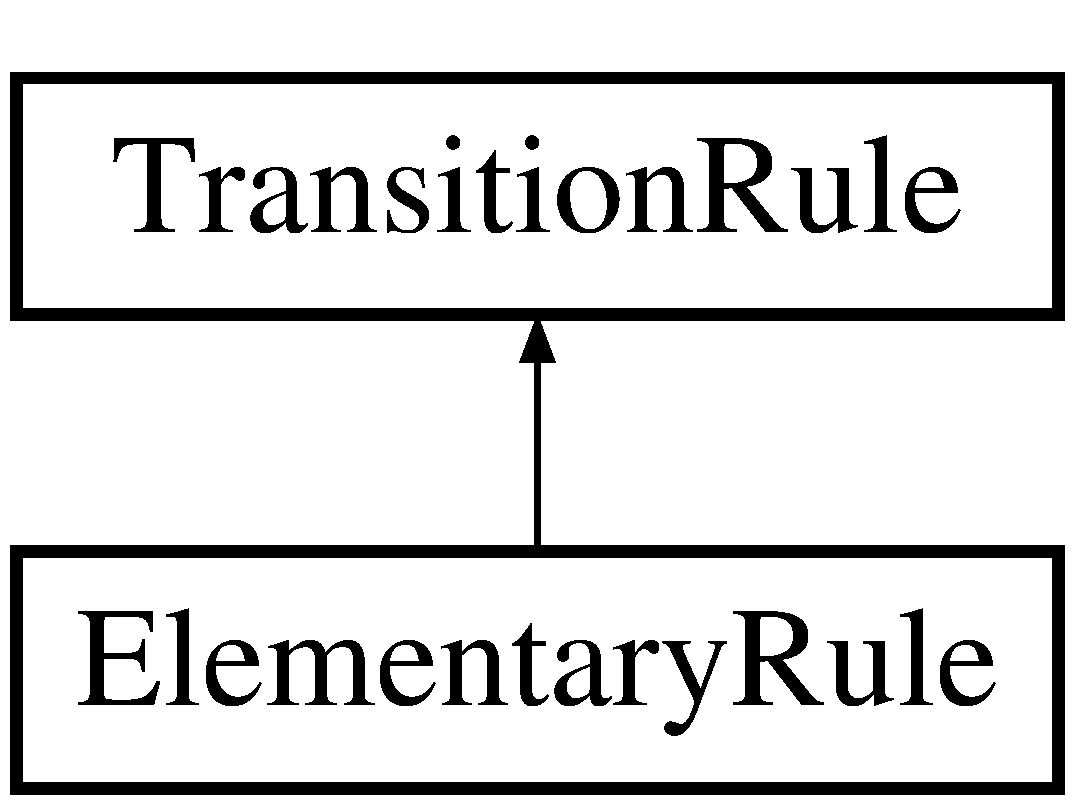
\includegraphics[height=3.000000cm]{class_elementary_rule}
\end{center}
\end{figure}
\subsection*{Public Member Functions}
\begin{DoxyCompactItemize}
\item 
\mbox{\Hypertarget{class_elementary_rule_a38451269153546c9d374f7f6df8cde6d}\label{class_elementary_rule_a38451269153546c9d374f7f6df8cde6d}} 
void {\bfseries Transition\+Cellule} (\mbox{\hyperlink{class_cell}{Cell}} const \&depart, \mbox{\hyperlink{class_cell}{Cell}} \&arrivee) const override
\item 
\mbox{\Hypertarget{class_elementary_rule_abcf6f8601c5ad393ee7e2a565e879f48}\label{class_elementary_rule_abcf6f8601c5ad393ee7e2a565e879f48}} 
{\bfseries Elementary\+Rule} (std\+::string rule, int nb\+Etats)
\end{DoxyCompactItemize}
\subsection*{Private Attributes}
\begin{DoxyCompactItemize}
\item 
\mbox{\Hypertarget{class_elementary_rule_a08733bd5dfc8395606006d513972f6c0}\label{class_elementary_rule_a08733bd5dfc8395606006d513972f6c0}} 
std\+::string {\bfseries m\+\_\+rule}
\item 
\mbox{\Hypertarget{class_elementary_rule_ade6ba3729cf8282c3b422a29b7c57a88}\label{class_elementary_rule_ade6ba3729cf8282c3b422a29b7c57a88}} 
int {\bfseries m\+\_\+nb\+Etats}
\end{DoxyCompactItemize}


The documentation for this class was generated from the following files\+:\begin{DoxyCompactItemize}
\item 
C\+:/\+Users/maxn0/git/\+L\+O21/\+Auto\+Cell/transitionrule.\+h\item 
C\+:/\+Users/maxn0/git/\+L\+O21/\+Auto\+Cell/transitionrule.\+cpp\end{DoxyCompactItemize}

\hypertarget{class_etat}{}\section{Etat Class Reference}
\label{class_etat}\index{Etat@{Etat}}
\subsection*{Public Member Functions}
\begin{DoxyCompactItemize}
\item 
\mbox{\Hypertarget{class_etat_a9de6f8f9bc1f9ec3296702a2ea9e7651}\label{class_etat_a9de6f8f9bc1f9ec3296702a2ea9e7651}} 
{\bfseries Etat} (int largeur, int longueur, \mbox{\hyperlink{class_generateur_etat}{Generateur\+Etat}} \&generateur, int nb\+Etats)
\item 
\mbox{\Hypertarget{class_etat_a4ab69207fc45fe1b193d3039eb456b32}\label{class_etat_a4ab69207fc45fe1b193d3039eb456b32}} 
{\bfseries Etat} (int largeur, int longueur, int $\ast$$\ast$tab)
\item 
\mbox{\Hypertarget{class_etat_a60fd78172b136c5011ccc840390ca378}\label{class_etat_a60fd78172b136c5011ccc840390ca378}} 
{\bfseries Etat} (int largeur, int longueur)
\item 
\mbox{\Hypertarget{class_etat_a6137bc65c74f615b6dca276ed1300e83}\label{class_etat_a6137bc65c74f615b6dca276ed1300e83}} 
{\bfseries Etat} (\mbox{\hyperlink{class_etat}{Etat}} const \&)=default
\item 
\mbox{\Hypertarget{class_etat_ad8cd3d55140d2b46784cb7623e998ee4}\label{class_etat_ad8cd3d55140d2b46784cb7623e998ee4}} 
void {\bfseries Regenerer} (int nb\+Etats)
\item 
\mbox{\Hypertarget{class_etat_a0ee4d5777ef97c1c7781e0e14b01699e}\label{class_etat_a0ee4d5777ef97c1c7781e0e14b01699e}} 
int {\bfseries Get\+Longueur} () const
\item 
\mbox{\Hypertarget{class_etat_a8dc404996c461e3cd4ebd301bfdcae4a}\label{class_etat_a8dc404996c461e3cd4ebd301bfdcae4a}} 
int {\bfseries Get\+Largeur} () const
\item 
\mbox{\Hypertarget{class_etat_a58c4c395d05101a68e8a28a8c1f769e9}\label{class_etat_a58c4c395d05101a68e8a28a8c1f769e9}} 
\mbox{\hyperlink{class_cell}{Cell}} const  \& {\bfseries Get\+Cellule} (int i, int j) const
\item 
\mbox{\Hypertarget{class_etat_addd390bbdb7b76148436a9a58c410f85}\label{class_etat_addd390bbdb7b76148436a9a58c410f85}} 
\mbox{\hyperlink{class_cell}{Cell}} \& {\bfseries Get\+Cellule} (int i, int j)
\item 
\mbox{\Hypertarget{class_etat_aeb0c23cfb166db846e567466dae0ebd1}\label{class_etat_aeb0c23cfb166db846e567466dae0ebd1}} 
void {\bfseries afficher} () const
\end{DoxyCompactItemize}
\subsection*{Private Attributes}
\begin{DoxyCompactItemize}
\item 
\mbox{\Hypertarget{class_etat_a914e5133fc90b6dc6b0bb31ea07aa1f0}\label{class_etat_a914e5133fc90b6dc6b0bb31ea07aa1f0}} 
\mbox{\hyperlink{class_generateur_etat}{Generateur\+Etat}} $\ast$ {\bfseries m\+\_\+generateur}
\item 
\mbox{\Hypertarget{class_etat_add8291e232f8219428147070f4126758}\label{class_etat_add8291e232f8219428147070f4126758}} 
std\+::vector$<$ std\+::vector$<$ \mbox{\hyperlink{class_cell}{Cell}} $>$ $>$ {\bfseries m\+\_\+cellules}
\item 
\mbox{\Hypertarget{class_etat_a2c443f1746c2e88a83ebeb15612aeea7}\label{class_etat_a2c443f1746c2e88a83ebeb15612aeea7}} 
int {\bfseries m\+\_\+longueur}
\item 
\mbox{\Hypertarget{class_etat_a227ad7e8e1bd5d692be7422444cb40d5}\label{class_etat_a227ad7e8e1bd5d692be7422444cb40d5}} 
int {\bfseries m\+\_\+largeur}
\end{DoxyCompactItemize}


The documentation for this class was generated from the following files\+:\begin{DoxyCompactItemize}
\item 
C\+:/\+Users/maxn0/git/\+L\+O21/\+Auto\+Cell/etat.\+h\item 
C\+:/\+Users/maxn0/git/\+L\+O21/\+Auto\+Cell/etat.\+cpp\end{DoxyCompactItemize}

\hypertarget{classfenetre1_d}{}\section{Référence de la classe fenetre1D}
\label{classfenetre1_d}\index{fenetre1D@{fenetre1D}}


{\ttfamily \#include $<$fenetre1d.\+h$>$}

Graphe d\textquotesingle{}héritage de fenetre1D\+:\begin{figure}[H]
\begin{center}
\leavevmode
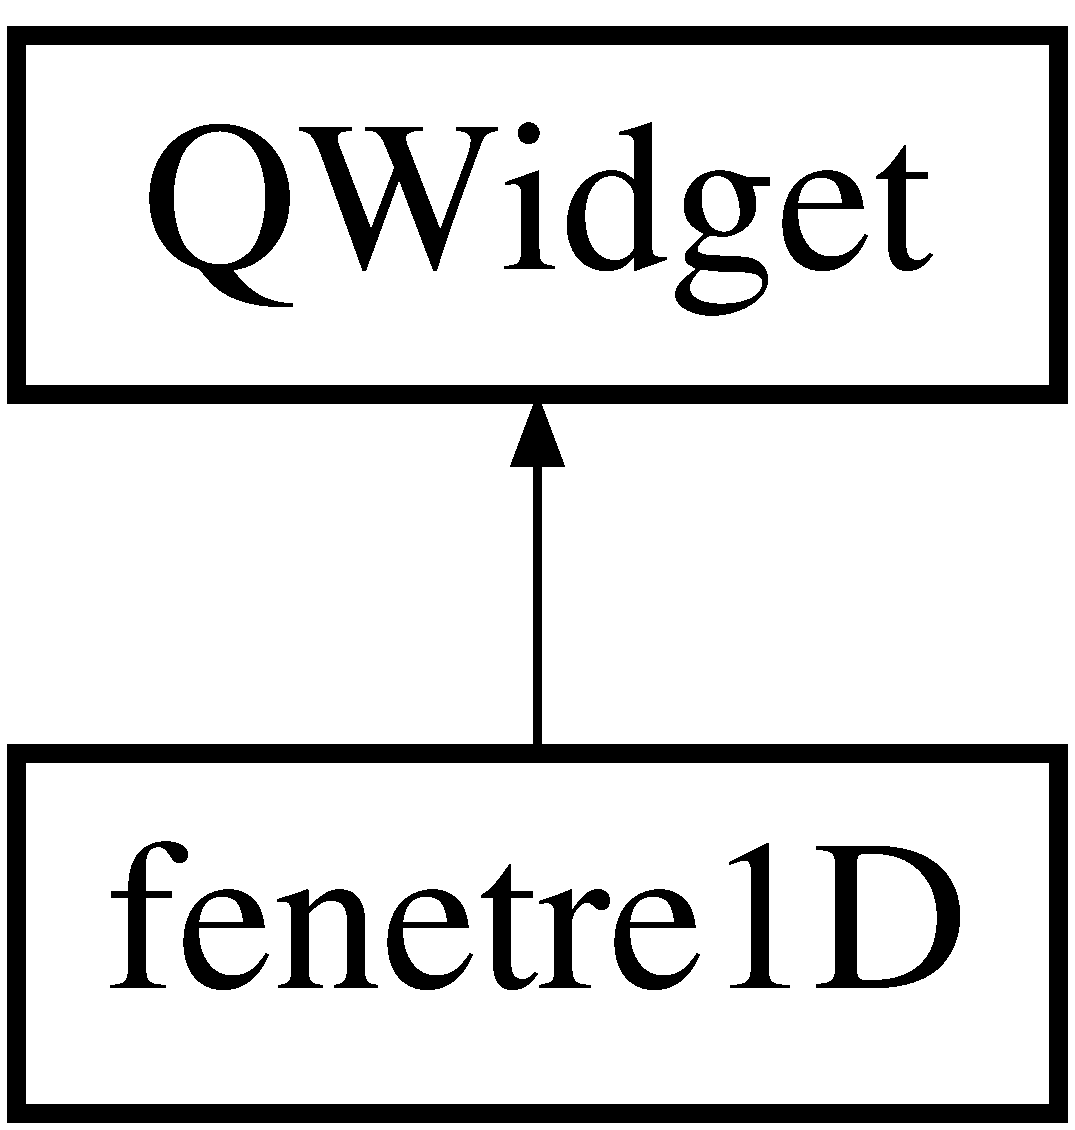
\includegraphics[height=2.000000cm]{classfenetre1_d}
\end{center}
\end{figure}
\subsection*{Fonctions membres publiques}
\begin{DoxyCompactItemize}
\item 
\mbox{\hyperlink{classfenetre1_d_adb843e57f0ba835052dfd216c82991ed}{fenetre1D}} (Q\+Widget $\ast$parent=nullptr)
\item 
\mbox{\hyperlink{classfenetre1_d_ad8ea627db7d11c383717afaa815f8dd0}{$\sim$fenetre1D}} ()
\item 
const \mbox{\hyperlink{class_cellular_automata}{Cellular\+Automata}} $\ast$ \mbox{\hyperlink{classfenetre1_d_a28ab62ea0d20e9f9dd5b3135a385314b}{get\+Simulateur}} () const
\item 
void \mbox{\hyperlink{classfenetre1_d_a13fdb7f89649288068f46b6aaf643053}{load\+Config}} ()
\item 
void \mbox{\hyperlink{classfenetre1_d_acc984ddd8dd83a65891a05b041614d21}{save\+Config}} ()
\end{DoxyCompactItemize}
\subsection*{Connecteurs privés}
\begin{DoxyCompactItemize}
\item 
void \mbox{\hyperlink{classfenetre1_d_a4ebfed6ec778e38de2039b077352d138}{cell\+Activation}} (const Q\+Model\+Index \&index)
\item 
void \mbox{\hyperlink{classfenetre1_d_a65b4806314f4a9ae06480579b94fde19}{build\+Grille}} ()
\item 
void \mbox{\hyperlink{classfenetre1_d_a26b1985ee0fdc3740a81844e38acd358}{generation\+Suivante}} ()
\item 
void \mbox{\hyperlink{classfenetre1_d_a30a0daefde3939596d4a4a4008a3e123}{play}} ()
\item 
void \mbox{\hyperlink{classfenetre1_d_af5560aef0fb4dd20062b3e27d18735b8}{pause}} ()
\item 
void \mbox{\hyperlink{classfenetre1_d_ac3be489fd45189bb7fb2a0170fc261ec}{appel\+Config}} () const
\item 
void \mbox{\hyperlink{classfenetre1_d_a32838578ed2cf59aa0fdb4115281ef3e}{Construire\+Etat}} ()
\item 
void \mbox{\hyperlink{classfenetre1_d_a8e06b057016afe1f0751493beb053107}{reset}} ()
\item 
void \mbox{\hyperlink{classfenetre1_d_a0f5127eb0216f22761ec7f57b8846cd8}{sauver\+Automate}} ()
\item 
void \mbox{\hyperlink{classfenetre1_d_a812d2a814c96979138174c04137aa4fd}{charger\+Automate}} ()
\item 
void \mbox{\hyperlink{classfenetre1_d_a120deb2f665cb65120c083d31c39a393}{sauver\+Etat}} ()
\item 
void \mbox{\hyperlink{classfenetre1_d_a4e7c8a38df8987fd216c355a163d6c46}{charger\+Etat}} ()
\item 
void \mbox{\hyperlink{classfenetre1_d_a3f9e0d5aaf29e45c7b04efb10ae450a1}{Construire\+Automate}} (int nb\+Etats=-\/1)
\end{DoxyCompactItemize}
\subsection*{Fonctions membres privées}
\begin{DoxyCompactItemize}
\item 
void \mbox{\hyperlink{classfenetre1_d_a8bf270f254fa50b992840f4b7d839893}{afficher\+Dernier\+Etat}} ()
\item 
void \mbox{\hyperlink{classfenetre1_d_a0af88e56b03b02ac2b1e7c44fe2699ce}{Construction\+Manuelle}} ()
\item 
void \mbox{\hyperlink{classfenetre1_d_aca92762c8a29d06ad95761dafce3a53f}{Update\+Info}} ()
\end{DoxyCompactItemize}
\subsection*{Attributs privés}
\begin{DoxyCompactItemize}
\item 
Q\+Push\+Button $\ast$ \mbox{\hyperlink{classfenetre1_d_a4e9511c51c66123628cebe3023867050}{b\+Generer\+Etat}}
\item 
Q\+Push\+Button $\ast$ \mbox{\hyperlink{classfenetre1_d_aae3db0f063b051302d8e18da12f9fcb2}{b\+Sauvegarder\+Etat}}
\item 
Q\+Push\+Button $\ast$ \mbox{\hyperlink{classfenetre1_d_ab12151af3a2e3f13d4513601db9fb368}{b\+Charger\+Etat}}
\item 
Q\+Spin\+Box $\ast$ \mbox{\hyperlink{classfenetre1_d_a024d9127c0ae5296d1c68d3c33b4c401}{b\+Largeur}}
\item 
Q\+Spin\+Box $\ast$ \mbox{\hyperlink{classfenetre1_d_ae84e79655e68b75cfe5185a54d4ca4eb}{b\+Longueur}}
\item 
Q\+Label $\ast$ \mbox{\hyperlink{classfenetre1_d_ada6a80288e77c9dbb1c014c159800850}{l\+Longueur}}
\item 
Q\+Label $\ast$ \mbox{\hyperlink{classfenetre1_d_adb30de1d87787ee16dec63d83803dde8}{l\+Largeur}}
\item 
Q\+Combo\+Box $\ast$ \mbox{\hyperlink{classfenetre1_d_a0bae0071f7bbf60ad635dd08fd5f1187}{bchoix\+Generateur}}
\item 
Q\+Table\+Widget $\ast$ \mbox{\hyperlink{classfenetre1_d_a42814a3d95f84cf0e0641f27bd863812}{depart}}
\item 
Q\+Table\+Widget $\ast$ \mbox{\hyperlink{classfenetre1_d_a429744707e605b19ce6d45bef34bc72e}{grille}}
\item 
Q\+Push\+Button $\ast$ \mbox{\hyperlink{classfenetre1_d_a9e0f7a6c615b709629e4604856776567}{b\+Start}}
\item 
Q\+Push\+Button $\ast$ \mbox{\hyperlink{classfenetre1_d_a39c09794926927cefe8aa7de36208f91}{b\+Pause}}
\item 
Q\+Push\+Button $\ast$ \mbox{\hyperlink{classfenetre1_d_aea5c5673c9078e25ab9870892b1f8f3f}{b\+Retour\+Depart}}
\item 
Q\+Push\+Button $\ast$ \mbox{\hyperlink{classfenetre1_d_ae00d1bc33bf3c829dceb250e53f8bb29}{b\+Next\+Frame}}
\item 
Q\+Spin\+Box $\ast$ \mbox{\hyperlink{classfenetre1_d_abd00cd8a248ece9ac867f073ead9aa83}{b\+Select\+Vitesse}}
\item 
Q\+Push\+Button $\ast$ \mbox{\hyperlink{classfenetre1_d_a355c71414f5f40cff800701a87d76068}{b\+Generer\+Automate}}
\item 
Q\+Push\+Button $\ast$ \mbox{\hyperlink{classfenetre1_d_a42db8c1238f6269c273174f5df0d7d41}{b\+Sauvegarder\+Automate}}
\item 
Q\+Push\+Button $\ast$ \mbox{\hyperlink{classfenetre1_d_a2c7730b0c732d1e35c4c3700c6400db4}{b\+Charger\+Automate}}
\item 
Q\+Combo\+Box $\ast$ \mbox{\hyperlink{classfenetre1_d_ae8ef06b7830dba2841ab6f74f4db31aa}{choix\+Automate}}
\item 
\mbox{\hyperlink{classfenetre_elementary_rule}{fenetre\+Elementary\+Rule}} $\ast$ \mbox{\hyperlink{classfenetre1_d_ad002647d7b1b7dc00e55cc2c72fe9678}{config\+Elementary\+Rule}}
\item 
\mbox{\hyperlink{class_cellular_automata}{Cellular\+Automata}} $\ast$ \mbox{\hyperlink{classfenetre1_d_a3eb4498daff2891b1f1a98a7cec26274}{simulateur}}
\item 
Q\+Timer $\ast$ \mbox{\hyperlink{classfenetre1_d_ad6bed04909cf6b10b5b944e370b5a0ef}{m\+\_\+timer}}
\item 
Q\+Label $\ast$ \mbox{\hyperlink{classfenetre1_d_afae5caa960edca0b17ed54681646432e}{m\+\_\+info}}
\end{DoxyCompactItemize}


\subsection{Documentation des constructeurs et destructeur}
\mbox{\Hypertarget{classfenetre1_d_adb843e57f0ba835052dfd216c82991ed}\label{classfenetre1_d_adb843e57f0ba835052dfd216c82991ed}} 
\index{fenetre1D@{fenetre1D}!fenetre1D@{fenetre1D}}
\index{fenetre1D@{fenetre1D}!fenetre1D@{fenetre1D}}
\subsubsection{\texorpdfstring{fenetre1\+D()}{fenetre1D()}}
{\footnotesize\ttfamily fenetre1\+D\+::fenetre1D (\begin{DoxyParamCaption}\item[{Q\+Widget $\ast$}]{parent = {\ttfamily nullptr} }\end{DoxyParamCaption})\hspace{0.3cm}{\ttfamily [explicit]}}

\mbox{\Hypertarget{classfenetre1_d_ad8ea627db7d11c383717afaa815f8dd0}\label{classfenetre1_d_ad8ea627db7d11c383717afaa815f8dd0}} 
\index{fenetre1D@{fenetre1D}!````~fenetre1D@{$\sim$fenetre1D}}
\index{````~fenetre1D@{$\sim$fenetre1D}!fenetre1D@{fenetre1D}}
\subsubsection{\texorpdfstring{$\sim$fenetre1\+D()}{~fenetre1D()}}
{\footnotesize\ttfamily fenetre1\+D\+::$\sim$fenetre1D (\begin{DoxyParamCaption}{ }\end{DoxyParamCaption})\hspace{0.3cm}{\ttfamily [inline]}}



\subsection{Documentation des fonctions membres}
\mbox{\Hypertarget{classfenetre1_d_a8bf270f254fa50b992840f4b7d839893}\label{classfenetre1_d_a8bf270f254fa50b992840f4b7d839893}} 
\index{fenetre1D@{fenetre1D}!afficher\+Dernier\+Etat@{afficher\+Dernier\+Etat}}
\index{afficher\+Dernier\+Etat@{afficher\+Dernier\+Etat}!fenetre1D@{fenetre1D}}
\subsubsection{\texorpdfstring{afficher\+Dernier\+Etat()}{afficherDernierEtat()}}
{\footnotesize\ttfamily void fenetre1\+D\+::afficher\+Dernier\+Etat (\begin{DoxyParamCaption}{ }\end{DoxyParamCaption})\hspace{0.3cm}{\ttfamily [private]}}

\mbox{\Hypertarget{classfenetre1_d_ac3be489fd45189bb7fb2a0170fc261ec}\label{classfenetre1_d_ac3be489fd45189bb7fb2a0170fc261ec}} 
\index{fenetre1D@{fenetre1D}!appel\+Config@{appel\+Config}}
\index{appel\+Config@{appel\+Config}!fenetre1D@{fenetre1D}}
\subsubsection{\texorpdfstring{appel\+Config}{appelConfig}}
{\footnotesize\ttfamily void fenetre1\+D\+::appel\+Config (\begin{DoxyParamCaption}{ }\end{DoxyParamCaption}) const\hspace{0.3cm}{\ttfamily [private]}, {\ttfamily [slot]}}

\mbox{\Hypertarget{classfenetre1_d_a65b4806314f4a9ae06480579b94fde19}\label{classfenetre1_d_a65b4806314f4a9ae06480579b94fde19}} 
\index{fenetre1D@{fenetre1D}!build\+Grille@{build\+Grille}}
\index{build\+Grille@{build\+Grille}!fenetre1D@{fenetre1D}}
\subsubsection{\texorpdfstring{build\+Grille}{buildGrille}}
{\footnotesize\ttfamily void fenetre1\+D\+::build\+Grille (\begin{DoxyParamCaption}{ }\end{DoxyParamCaption})\hspace{0.3cm}{\ttfamily [private]}, {\ttfamily [slot]}}

\mbox{\Hypertarget{classfenetre1_d_a4ebfed6ec778e38de2039b077352d138}\label{classfenetre1_d_a4ebfed6ec778e38de2039b077352d138}} 
\index{fenetre1D@{fenetre1D}!cell\+Activation@{cell\+Activation}}
\index{cell\+Activation@{cell\+Activation}!fenetre1D@{fenetre1D}}
\subsubsection{\texorpdfstring{cell\+Activation}{cellActivation}}
{\footnotesize\ttfamily void fenetre1\+D\+::cell\+Activation (\begin{DoxyParamCaption}\item[{const Q\+Model\+Index \&}]{index }\end{DoxyParamCaption})\hspace{0.3cm}{\ttfamily [private]}, {\ttfamily [slot]}}

\mbox{\Hypertarget{classfenetre1_d_a812d2a814c96979138174c04137aa4fd}\label{classfenetre1_d_a812d2a814c96979138174c04137aa4fd}} 
\index{fenetre1D@{fenetre1D}!charger\+Automate@{charger\+Automate}}
\index{charger\+Automate@{charger\+Automate}!fenetre1D@{fenetre1D}}
\subsubsection{\texorpdfstring{charger\+Automate}{chargerAutomate}}
{\footnotesize\ttfamily void fenetre1\+D\+::charger\+Automate (\begin{DoxyParamCaption}{ }\end{DoxyParamCaption})\hspace{0.3cm}{\ttfamily [private]}, {\ttfamily [slot]}}

\mbox{\Hypertarget{classfenetre1_d_a4e7c8a38df8987fd216c355a163d6c46}\label{classfenetre1_d_a4e7c8a38df8987fd216c355a163d6c46}} 
\index{fenetre1D@{fenetre1D}!charger\+Etat@{charger\+Etat}}
\index{charger\+Etat@{charger\+Etat}!fenetre1D@{fenetre1D}}
\subsubsection{\texorpdfstring{charger\+Etat}{chargerEtat}}
{\footnotesize\ttfamily void fenetre1\+D\+::charger\+Etat (\begin{DoxyParamCaption}{ }\end{DoxyParamCaption})\hspace{0.3cm}{\ttfamily [private]}, {\ttfamily [slot]}}

\mbox{\Hypertarget{classfenetre1_d_a0af88e56b03b02ac2b1e7c44fe2699ce}\label{classfenetre1_d_a0af88e56b03b02ac2b1e7c44fe2699ce}} 
\index{fenetre1D@{fenetre1D}!Construction\+Manuelle@{Construction\+Manuelle}}
\index{Construction\+Manuelle@{Construction\+Manuelle}!fenetre1D@{fenetre1D}}
\subsubsection{\texorpdfstring{Construction\+Manuelle()}{ConstructionManuelle()}}
{\footnotesize\ttfamily void fenetre1\+D\+::\+Construction\+Manuelle (\begin{DoxyParamCaption}{ }\end{DoxyParamCaption})\hspace{0.3cm}{\ttfamily [private]}}

\mbox{\Hypertarget{classfenetre1_d_a3f9e0d5aaf29e45c7b04efb10ae450a1}\label{classfenetre1_d_a3f9e0d5aaf29e45c7b04efb10ae450a1}} 
\index{fenetre1D@{fenetre1D}!Construire\+Automate@{Construire\+Automate}}
\index{Construire\+Automate@{Construire\+Automate}!fenetre1D@{fenetre1D}}
\subsubsection{\texorpdfstring{Construire\+Automate}{ConstruireAutomate}}
{\footnotesize\ttfamily void fenetre1\+D\+::\+Construire\+Automate (\begin{DoxyParamCaption}\item[{int}]{nb\+Etats = {\ttfamily -\/1} }\end{DoxyParamCaption})\hspace{0.3cm}{\ttfamily [private]}, {\ttfamily [slot]}}

\mbox{\Hypertarget{classfenetre1_d_a32838578ed2cf59aa0fdb4115281ef3e}\label{classfenetre1_d_a32838578ed2cf59aa0fdb4115281ef3e}} 
\index{fenetre1D@{fenetre1D}!Construire\+Etat@{Construire\+Etat}}
\index{Construire\+Etat@{Construire\+Etat}!fenetre1D@{fenetre1D}}
\subsubsection{\texorpdfstring{Construire\+Etat}{ConstruireEtat}}
{\footnotesize\ttfamily void fenetre1\+D\+::\+Construire\+Etat (\begin{DoxyParamCaption}{ }\end{DoxyParamCaption})\hspace{0.3cm}{\ttfamily [private]}, {\ttfamily [slot]}}

\mbox{\Hypertarget{classfenetre1_d_a26b1985ee0fdc3740a81844e38acd358}\label{classfenetre1_d_a26b1985ee0fdc3740a81844e38acd358}} 
\index{fenetre1D@{fenetre1D}!generation\+Suivante@{generation\+Suivante}}
\index{generation\+Suivante@{generation\+Suivante}!fenetre1D@{fenetre1D}}
\subsubsection{\texorpdfstring{generation\+Suivante}{generationSuivante}}
{\footnotesize\ttfamily void fenetre1\+D\+::generation\+Suivante (\begin{DoxyParamCaption}{ }\end{DoxyParamCaption})\hspace{0.3cm}{\ttfamily [private]}, {\ttfamily [slot]}}

\mbox{\Hypertarget{classfenetre1_d_a28ab62ea0d20e9f9dd5b3135a385314b}\label{classfenetre1_d_a28ab62ea0d20e9f9dd5b3135a385314b}} 
\index{fenetre1D@{fenetre1D}!get\+Simulateur@{get\+Simulateur}}
\index{get\+Simulateur@{get\+Simulateur}!fenetre1D@{fenetre1D}}
\subsubsection{\texorpdfstring{get\+Simulateur()}{getSimulateur()}}
{\footnotesize\ttfamily const \mbox{\hyperlink{class_cellular_automata}{Cellular\+Automata}} $\ast$ fenetre1\+D\+::get\+Simulateur (\begin{DoxyParamCaption}{ }\end{DoxyParamCaption}) const}

\mbox{\Hypertarget{classfenetre1_d_a13fdb7f89649288068f46b6aaf643053}\label{classfenetre1_d_a13fdb7f89649288068f46b6aaf643053}} 
\index{fenetre1D@{fenetre1D}!load\+Config@{load\+Config}}
\index{load\+Config@{load\+Config}!fenetre1D@{fenetre1D}}
\subsubsection{\texorpdfstring{load\+Config()}{loadConfig()}}
{\footnotesize\ttfamily void fenetre1\+D\+::load\+Config (\begin{DoxyParamCaption}{ }\end{DoxyParamCaption})}

\mbox{\Hypertarget{classfenetre1_d_af5560aef0fb4dd20062b3e27d18735b8}\label{classfenetre1_d_af5560aef0fb4dd20062b3e27d18735b8}} 
\index{fenetre1D@{fenetre1D}!pause@{pause}}
\index{pause@{pause}!fenetre1D@{fenetre1D}}
\subsubsection{\texorpdfstring{pause}{pause}}
{\footnotesize\ttfamily void fenetre1\+D\+::pause (\begin{DoxyParamCaption}{ }\end{DoxyParamCaption})\hspace{0.3cm}{\ttfamily [private]}, {\ttfamily [slot]}}

\mbox{\Hypertarget{classfenetre1_d_a30a0daefde3939596d4a4a4008a3e123}\label{classfenetre1_d_a30a0daefde3939596d4a4a4008a3e123}} 
\index{fenetre1D@{fenetre1D}!play@{play}}
\index{play@{play}!fenetre1D@{fenetre1D}}
\subsubsection{\texorpdfstring{play}{play}}
{\footnotesize\ttfamily void fenetre1\+D\+::play (\begin{DoxyParamCaption}{ }\end{DoxyParamCaption})\hspace{0.3cm}{\ttfamily [private]}, {\ttfamily [slot]}}

\mbox{\Hypertarget{classfenetre1_d_a8e06b057016afe1f0751493beb053107}\label{classfenetre1_d_a8e06b057016afe1f0751493beb053107}} 
\index{fenetre1D@{fenetre1D}!reset@{reset}}
\index{reset@{reset}!fenetre1D@{fenetre1D}}
\subsubsection{\texorpdfstring{reset}{reset}}
{\footnotesize\ttfamily void fenetre1\+D\+::reset (\begin{DoxyParamCaption}{ }\end{DoxyParamCaption})\hspace{0.3cm}{\ttfamily [private]}, {\ttfamily [slot]}}

\mbox{\Hypertarget{classfenetre1_d_a0f5127eb0216f22761ec7f57b8846cd8}\label{classfenetre1_d_a0f5127eb0216f22761ec7f57b8846cd8}} 
\index{fenetre1D@{fenetre1D}!sauver\+Automate@{sauver\+Automate}}
\index{sauver\+Automate@{sauver\+Automate}!fenetre1D@{fenetre1D}}
\subsubsection{\texorpdfstring{sauver\+Automate}{sauverAutomate}}
{\footnotesize\ttfamily void fenetre1\+D\+::sauver\+Automate (\begin{DoxyParamCaption}{ }\end{DoxyParamCaption})\hspace{0.3cm}{\ttfamily [private]}, {\ttfamily [slot]}}

\mbox{\Hypertarget{classfenetre1_d_a120deb2f665cb65120c083d31c39a393}\label{classfenetre1_d_a120deb2f665cb65120c083d31c39a393}} 
\index{fenetre1D@{fenetre1D}!sauver\+Etat@{sauver\+Etat}}
\index{sauver\+Etat@{sauver\+Etat}!fenetre1D@{fenetre1D}}
\subsubsection{\texorpdfstring{sauver\+Etat}{sauverEtat}}
{\footnotesize\ttfamily void fenetre1\+D\+::sauver\+Etat (\begin{DoxyParamCaption}{ }\end{DoxyParamCaption})\hspace{0.3cm}{\ttfamily [private]}, {\ttfamily [slot]}}

\mbox{\Hypertarget{classfenetre1_d_acc984ddd8dd83a65891a05b041614d21}\label{classfenetre1_d_acc984ddd8dd83a65891a05b041614d21}} 
\index{fenetre1D@{fenetre1D}!save\+Config@{save\+Config}}
\index{save\+Config@{save\+Config}!fenetre1D@{fenetre1D}}
\subsubsection{\texorpdfstring{save\+Config()}{saveConfig()}}
{\footnotesize\ttfamily void fenetre1\+D\+::save\+Config (\begin{DoxyParamCaption}{ }\end{DoxyParamCaption})}

\mbox{\Hypertarget{classfenetre1_d_aca92762c8a29d06ad95761dafce3a53f}\label{classfenetre1_d_aca92762c8a29d06ad95761dafce3a53f}} 
\index{fenetre1D@{fenetre1D}!Update\+Info@{Update\+Info}}
\index{Update\+Info@{Update\+Info}!fenetre1D@{fenetre1D}}
\subsubsection{\texorpdfstring{Update\+Info()}{UpdateInfo()}}
{\footnotesize\ttfamily void fenetre1\+D\+::\+Update\+Info (\begin{DoxyParamCaption}{ }\end{DoxyParamCaption})\hspace{0.3cm}{\ttfamily [private]}}



\subsection{Documentation des données membres}
\mbox{\Hypertarget{classfenetre1_d_a2c7730b0c732d1e35c4c3700c6400db4}\label{classfenetre1_d_a2c7730b0c732d1e35c4c3700c6400db4}} 
\index{fenetre1D@{fenetre1D}!b\+Charger\+Automate@{b\+Charger\+Automate}}
\index{b\+Charger\+Automate@{b\+Charger\+Automate}!fenetre1D@{fenetre1D}}
\subsubsection{\texorpdfstring{b\+Charger\+Automate}{bChargerAutomate}}
{\footnotesize\ttfamily Q\+Push\+Button$\ast$ fenetre1\+D\+::b\+Charger\+Automate\hspace{0.3cm}{\ttfamily [private]}}

\mbox{\Hypertarget{classfenetre1_d_ab12151af3a2e3f13d4513601db9fb368}\label{classfenetre1_d_ab12151af3a2e3f13d4513601db9fb368}} 
\index{fenetre1D@{fenetre1D}!b\+Charger\+Etat@{b\+Charger\+Etat}}
\index{b\+Charger\+Etat@{b\+Charger\+Etat}!fenetre1D@{fenetre1D}}
\subsubsection{\texorpdfstring{b\+Charger\+Etat}{bChargerEtat}}
{\footnotesize\ttfamily Q\+Push\+Button$\ast$ fenetre1\+D\+::b\+Charger\+Etat\hspace{0.3cm}{\ttfamily [private]}}

\mbox{\Hypertarget{classfenetre1_d_a0bae0071f7bbf60ad635dd08fd5f1187}\label{classfenetre1_d_a0bae0071f7bbf60ad635dd08fd5f1187}} 
\index{fenetre1D@{fenetre1D}!bchoix\+Generateur@{bchoix\+Generateur}}
\index{bchoix\+Generateur@{bchoix\+Generateur}!fenetre1D@{fenetre1D}}
\subsubsection{\texorpdfstring{bchoix\+Generateur}{bchoixGenerateur}}
{\footnotesize\ttfamily Q\+Combo\+Box$\ast$ fenetre1\+D\+::bchoix\+Generateur\hspace{0.3cm}{\ttfamily [private]}}

\mbox{\Hypertarget{classfenetre1_d_a355c71414f5f40cff800701a87d76068}\label{classfenetre1_d_a355c71414f5f40cff800701a87d76068}} 
\index{fenetre1D@{fenetre1D}!b\+Generer\+Automate@{b\+Generer\+Automate}}
\index{b\+Generer\+Automate@{b\+Generer\+Automate}!fenetre1D@{fenetre1D}}
\subsubsection{\texorpdfstring{b\+Generer\+Automate}{bGenererAutomate}}
{\footnotesize\ttfamily Q\+Push\+Button$\ast$ fenetre1\+D\+::b\+Generer\+Automate\hspace{0.3cm}{\ttfamily [private]}}

\mbox{\Hypertarget{classfenetre1_d_a4e9511c51c66123628cebe3023867050}\label{classfenetre1_d_a4e9511c51c66123628cebe3023867050}} 
\index{fenetre1D@{fenetre1D}!b\+Generer\+Etat@{b\+Generer\+Etat}}
\index{b\+Generer\+Etat@{b\+Generer\+Etat}!fenetre1D@{fenetre1D}}
\subsubsection{\texorpdfstring{b\+Generer\+Etat}{bGenererEtat}}
{\footnotesize\ttfamily Q\+Push\+Button$\ast$ fenetre1\+D\+::b\+Generer\+Etat\hspace{0.3cm}{\ttfamily [private]}}

\mbox{\Hypertarget{classfenetre1_d_a024d9127c0ae5296d1c68d3c33b4c401}\label{classfenetre1_d_a024d9127c0ae5296d1c68d3c33b4c401}} 
\index{fenetre1D@{fenetre1D}!b\+Largeur@{b\+Largeur}}
\index{b\+Largeur@{b\+Largeur}!fenetre1D@{fenetre1D}}
\subsubsection{\texorpdfstring{b\+Largeur}{bLargeur}}
{\footnotesize\ttfamily Q\+Spin\+Box$\ast$ fenetre1\+D\+::b\+Largeur\hspace{0.3cm}{\ttfamily [private]}}

\mbox{\Hypertarget{classfenetre1_d_ae84e79655e68b75cfe5185a54d4ca4eb}\label{classfenetre1_d_ae84e79655e68b75cfe5185a54d4ca4eb}} 
\index{fenetre1D@{fenetre1D}!b\+Longueur@{b\+Longueur}}
\index{b\+Longueur@{b\+Longueur}!fenetre1D@{fenetre1D}}
\subsubsection{\texorpdfstring{b\+Longueur}{bLongueur}}
{\footnotesize\ttfamily Q\+Spin\+Box$\ast$ fenetre1\+D\+::b\+Longueur\hspace{0.3cm}{\ttfamily [private]}}

\mbox{\Hypertarget{classfenetre1_d_ae00d1bc33bf3c829dceb250e53f8bb29}\label{classfenetre1_d_ae00d1bc33bf3c829dceb250e53f8bb29}} 
\index{fenetre1D@{fenetre1D}!b\+Next\+Frame@{b\+Next\+Frame}}
\index{b\+Next\+Frame@{b\+Next\+Frame}!fenetre1D@{fenetre1D}}
\subsubsection{\texorpdfstring{b\+Next\+Frame}{bNextFrame}}
{\footnotesize\ttfamily Q\+Push\+Button$\ast$ fenetre1\+D\+::b\+Next\+Frame\hspace{0.3cm}{\ttfamily [private]}}

\mbox{\Hypertarget{classfenetre1_d_a39c09794926927cefe8aa7de36208f91}\label{classfenetre1_d_a39c09794926927cefe8aa7de36208f91}} 
\index{fenetre1D@{fenetre1D}!b\+Pause@{b\+Pause}}
\index{b\+Pause@{b\+Pause}!fenetre1D@{fenetre1D}}
\subsubsection{\texorpdfstring{b\+Pause}{bPause}}
{\footnotesize\ttfamily Q\+Push\+Button$\ast$ fenetre1\+D\+::b\+Pause\hspace{0.3cm}{\ttfamily [private]}}

\mbox{\Hypertarget{classfenetre1_d_aea5c5673c9078e25ab9870892b1f8f3f}\label{classfenetre1_d_aea5c5673c9078e25ab9870892b1f8f3f}} 
\index{fenetre1D@{fenetre1D}!b\+Retour\+Depart@{b\+Retour\+Depart}}
\index{b\+Retour\+Depart@{b\+Retour\+Depart}!fenetre1D@{fenetre1D}}
\subsubsection{\texorpdfstring{b\+Retour\+Depart}{bRetourDepart}}
{\footnotesize\ttfamily Q\+Push\+Button$\ast$ fenetre1\+D\+::b\+Retour\+Depart\hspace{0.3cm}{\ttfamily [private]}}

\mbox{\Hypertarget{classfenetre1_d_a42db8c1238f6269c273174f5df0d7d41}\label{classfenetre1_d_a42db8c1238f6269c273174f5df0d7d41}} 
\index{fenetre1D@{fenetre1D}!b\+Sauvegarder\+Automate@{b\+Sauvegarder\+Automate}}
\index{b\+Sauvegarder\+Automate@{b\+Sauvegarder\+Automate}!fenetre1D@{fenetre1D}}
\subsubsection{\texorpdfstring{b\+Sauvegarder\+Automate}{bSauvegarderAutomate}}
{\footnotesize\ttfamily Q\+Push\+Button$\ast$ fenetre1\+D\+::b\+Sauvegarder\+Automate\hspace{0.3cm}{\ttfamily [private]}}

\mbox{\Hypertarget{classfenetre1_d_aae3db0f063b051302d8e18da12f9fcb2}\label{classfenetre1_d_aae3db0f063b051302d8e18da12f9fcb2}} 
\index{fenetre1D@{fenetre1D}!b\+Sauvegarder\+Etat@{b\+Sauvegarder\+Etat}}
\index{b\+Sauvegarder\+Etat@{b\+Sauvegarder\+Etat}!fenetre1D@{fenetre1D}}
\subsubsection{\texorpdfstring{b\+Sauvegarder\+Etat}{bSauvegarderEtat}}
{\footnotesize\ttfamily Q\+Push\+Button$\ast$ fenetre1\+D\+::b\+Sauvegarder\+Etat\hspace{0.3cm}{\ttfamily [private]}}

\mbox{\Hypertarget{classfenetre1_d_abd00cd8a248ece9ac867f073ead9aa83}\label{classfenetre1_d_abd00cd8a248ece9ac867f073ead9aa83}} 
\index{fenetre1D@{fenetre1D}!b\+Select\+Vitesse@{b\+Select\+Vitesse}}
\index{b\+Select\+Vitesse@{b\+Select\+Vitesse}!fenetre1D@{fenetre1D}}
\subsubsection{\texorpdfstring{b\+Select\+Vitesse}{bSelectVitesse}}
{\footnotesize\ttfamily Q\+Spin\+Box$\ast$ fenetre1\+D\+::b\+Select\+Vitesse\hspace{0.3cm}{\ttfamily [private]}}

\mbox{\Hypertarget{classfenetre1_d_a9e0f7a6c615b709629e4604856776567}\label{classfenetre1_d_a9e0f7a6c615b709629e4604856776567}} 
\index{fenetre1D@{fenetre1D}!b\+Start@{b\+Start}}
\index{b\+Start@{b\+Start}!fenetre1D@{fenetre1D}}
\subsubsection{\texorpdfstring{b\+Start}{bStart}}
{\footnotesize\ttfamily Q\+Push\+Button$\ast$ fenetre1\+D\+::b\+Start\hspace{0.3cm}{\ttfamily [private]}}

\mbox{\Hypertarget{classfenetre1_d_ae8ef06b7830dba2841ab6f74f4db31aa}\label{classfenetre1_d_ae8ef06b7830dba2841ab6f74f4db31aa}} 
\index{fenetre1D@{fenetre1D}!choix\+Automate@{choix\+Automate}}
\index{choix\+Automate@{choix\+Automate}!fenetre1D@{fenetre1D}}
\subsubsection{\texorpdfstring{choix\+Automate}{choixAutomate}}
{\footnotesize\ttfamily Q\+Combo\+Box$\ast$ fenetre1\+D\+::choix\+Automate\hspace{0.3cm}{\ttfamily [private]}}

\mbox{\Hypertarget{classfenetre1_d_ad002647d7b1b7dc00e55cc2c72fe9678}\label{classfenetre1_d_ad002647d7b1b7dc00e55cc2c72fe9678}} 
\index{fenetre1D@{fenetre1D}!config\+Elementary\+Rule@{config\+Elementary\+Rule}}
\index{config\+Elementary\+Rule@{config\+Elementary\+Rule}!fenetre1D@{fenetre1D}}
\subsubsection{\texorpdfstring{config\+Elementary\+Rule}{configElementaryRule}}
{\footnotesize\ttfamily \mbox{\hyperlink{classfenetre_elementary_rule}{fenetre\+Elementary\+Rule}}$\ast$ fenetre1\+D\+::config\+Elementary\+Rule\hspace{0.3cm}{\ttfamily [private]}}

\mbox{\Hypertarget{classfenetre1_d_a42814a3d95f84cf0e0641f27bd863812}\label{classfenetre1_d_a42814a3d95f84cf0e0641f27bd863812}} 
\index{fenetre1D@{fenetre1D}!depart@{depart}}
\index{depart@{depart}!fenetre1D@{fenetre1D}}
\subsubsection{\texorpdfstring{depart}{depart}}
{\footnotesize\ttfamily Q\+Table\+Widget$\ast$ fenetre1\+D\+::depart\hspace{0.3cm}{\ttfamily [private]}}

\mbox{\Hypertarget{classfenetre1_d_a429744707e605b19ce6d45bef34bc72e}\label{classfenetre1_d_a429744707e605b19ce6d45bef34bc72e}} 
\index{fenetre1D@{fenetre1D}!grille@{grille}}
\index{grille@{grille}!fenetre1D@{fenetre1D}}
\subsubsection{\texorpdfstring{grille}{grille}}
{\footnotesize\ttfamily Q\+Table\+Widget$\ast$ fenetre1\+D\+::grille\hspace{0.3cm}{\ttfamily [private]}}

\mbox{\Hypertarget{classfenetre1_d_adb30de1d87787ee16dec63d83803dde8}\label{classfenetre1_d_adb30de1d87787ee16dec63d83803dde8}} 
\index{fenetre1D@{fenetre1D}!l\+Largeur@{l\+Largeur}}
\index{l\+Largeur@{l\+Largeur}!fenetre1D@{fenetre1D}}
\subsubsection{\texorpdfstring{l\+Largeur}{lLargeur}}
{\footnotesize\ttfamily Q\+Label$\ast$ fenetre1\+D\+::l\+Largeur\hspace{0.3cm}{\ttfamily [private]}}

\mbox{\Hypertarget{classfenetre1_d_ada6a80288e77c9dbb1c014c159800850}\label{classfenetre1_d_ada6a80288e77c9dbb1c014c159800850}} 
\index{fenetre1D@{fenetre1D}!l\+Longueur@{l\+Longueur}}
\index{l\+Longueur@{l\+Longueur}!fenetre1D@{fenetre1D}}
\subsubsection{\texorpdfstring{l\+Longueur}{lLongueur}}
{\footnotesize\ttfamily Q\+Label$\ast$ fenetre1\+D\+::l\+Longueur\hspace{0.3cm}{\ttfamily [private]}}

\mbox{\Hypertarget{classfenetre1_d_afae5caa960edca0b17ed54681646432e}\label{classfenetre1_d_afae5caa960edca0b17ed54681646432e}} 
\index{fenetre1D@{fenetre1D}!m\+\_\+info@{m\+\_\+info}}
\index{m\+\_\+info@{m\+\_\+info}!fenetre1D@{fenetre1D}}
\subsubsection{\texorpdfstring{m\+\_\+info}{m\_info}}
{\footnotesize\ttfamily Q\+Label$\ast$ fenetre1\+D\+::m\+\_\+info\hspace{0.3cm}{\ttfamily [private]}}

\mbox{\Hypertarget{classfenetre1_d_ad6bed04909cf6b10b5b944e370b5a0ef}\label{classfenetre1_d_ad6bed04909cf6b10b5b944e370b5a0ef}} 
\index{fenetre1D@{fenetre1D}!m\+\_\+timer@{m\+\_\+timer}}
\index{m\+\_\+timer@{m\+\_\+timer}!fenetre1D@{fenetre1D}}
\subsubsection{\texorpdfstring{m\+\_\+timer}{m\_timer}}
{\footnotesize\ttfamily Q\+Timer$\ast$ fenetre1\+D\+::m\+\_\+timer\hspace{0.3cm}{\ttfamily [private]}}

\mbox{\Hypertarget{classfenetre1_d_a3eb4498daff2891b1f1a98a7cec26274}\label{classfenetre1_d_a3eb4498daff2891b1f1a98a7cec26274}} 
\index{fenetre1D@{fenetre1D}!simulateur@{simulateur}}
\index{simulateur@{simulateur}!fenetre1D@{fenetre1D}}
\subsubsection{\texorpdfstring{simulateur}{simulateur}}
{\footnotesize\ttfamily \mbox{\hyperlink{class_cellular_automata}{Cellular\+Automata}}$\ast$ fenetre1\+D\+::simulateur\hspace{0.3cm}{\ttfamily [private]}}



La documentation de cette classe a été générée à partir des fichiers suivants \+:\begin{DoxyCompactItemize}
\item 
C\+:/\+Users/maxn0/git/\+L\+O21/\+Auto\+Cell/\mbox{\hyperlink{fenetre1d_8h}{fenetre1d.\+h}}\item 
C\+:/\+Users/maxn0/git/\+L\+O21/\+Auto\+Cell/\mbox{\hyperlink{fenetre1d_8cpp}{fenetre1d.\+cpp}}\end{DoxyCompactItemize}

\hypertarget{classfenetre2_d}{}\section{Référence de la classe fenetre2D}
\label{classfenetre2_d}\index{fenetre2D@{fenetre2D}}


{\ttfamily \#include $<$fenetre2d.\+h$>$}

Graphe d\textquotesingle{}héritage de fenetre2D\+:\begin{figure}[H]
\begin{center}
\leavevmode
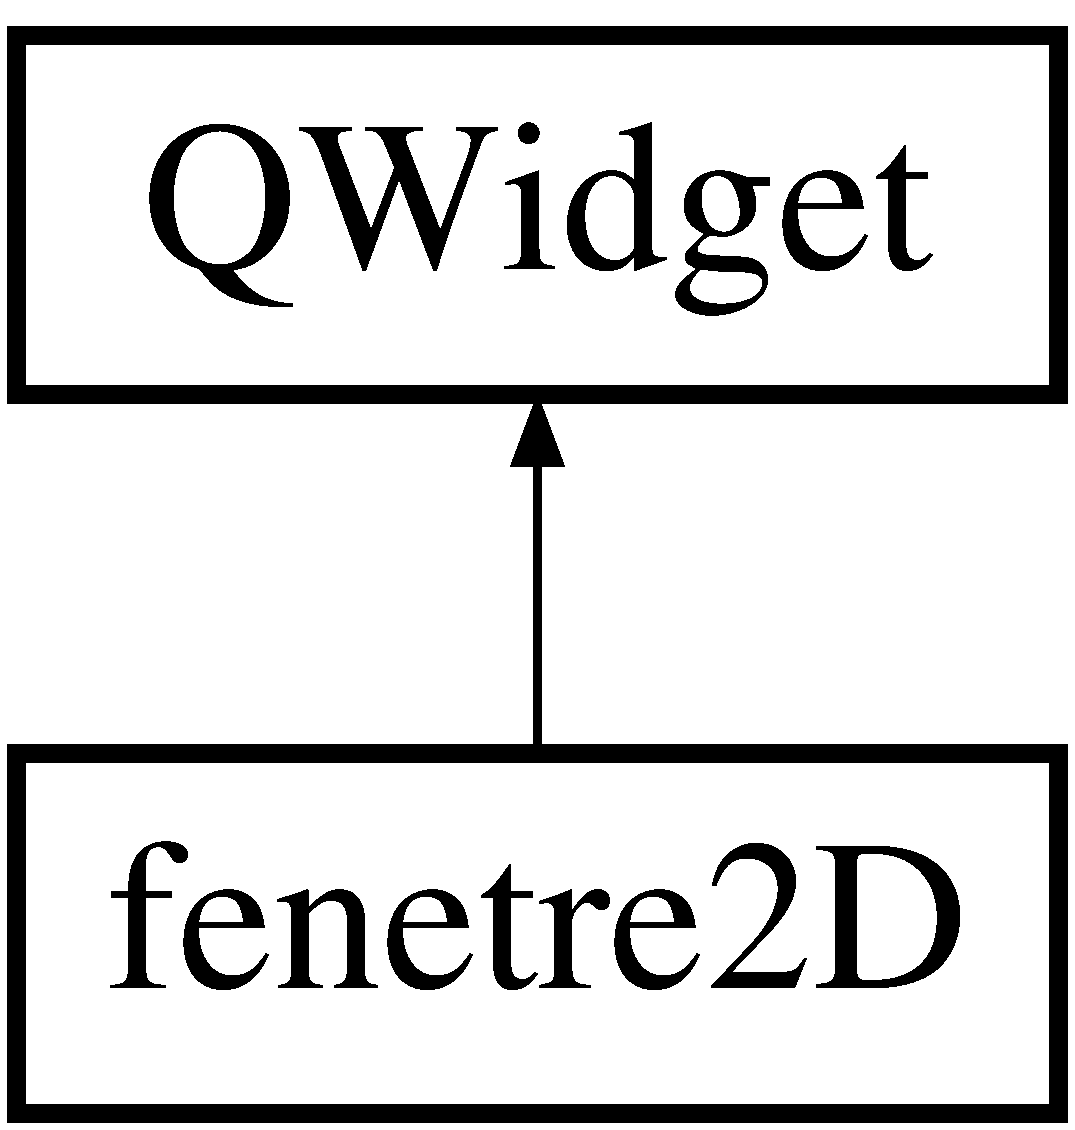
\includegraphics[height=2.000000cm]{classfenetre2_d}
\end{center}
\end{figure}
\subsection*{Fonctions membres publiques}
\begin{DoxyCompactItemize}
\item 
\mbox{\hyperlink{classfenetre2_d_af1d21292db6ff26d9746374c916039a4}{fenetre2D}} (Q\+Widget $\ast$parent=nullptr)
\item 
\mbox{\hyperlink{classfenetre2_d_a2638afe65581b117673f7133cfbbdc9c}{$\sim$fenetre2D}} ()
\item 
const \mbox{\hyperlink{class_cellular_automata}{Cellular\+Automata}} $\ast$ \mbox{\hyperlink{classfenetre2_d_ab8e5b79b50a28c663bde2e83a202d80c}{get\+Simulateur}} () const
\item 
void \mbox{\hyperlink{classfenetre2_d_a9ee93dcc5e0e7ee3ddcf4bd4bb967162}{load\+Config}} ()
\item 
void \mbox{\hyperlink{classfenetre2_d_a5ac8e27ac8642c78fc40af3afb0a91cd}{save\+Config}} ()
\end{DoxyCompactItemize}
\subsection*{Connecteurs privés}
\begin{DoxyCompactItemize}
\item 
void \mbox{\hyperlink{classfenetre2_d_abb32f8f446b8e4fd1b0d0dc35cf9286e}{cell\+Activation}} (const Q\+Model\+Index \&index)
\item 
void \mbox{\hyperlink{classfenetre2_d_a63ca9b8bcfad281fc0180d93f5ca0f18}{build\+Grille}} ()
\item 
void \mbox{\hyperlink{classfenetre2_d_a643866b152510c7a80412a084248eb7d}{generation\+Suivante}} ()
\item 
void \mbox{\hyperlink{classfenetre2_d_a8cba1977fee440949f2711bbc15f7f63}{play}} ()
\item 
void \mbox{\hyperlink{classfenetre2_d_adbc8e3e644842494a6512373e0b82a98}{pause}} ()
\item 
void \mbox{\hyperlink{classfenetre2_d_aa624848d78b19079259e7c9f5c90842f}{appel\+Config}} () const
\item 
void \mbox{\hyperlink{classfenetre2_d_a3824878eb7b51b5137d16c969e380861}{Construire\+Etat}} ()
\item 
void \mbox{\hyperlink{classfenetre2_d_a5f143e0cff9013924179309bb25a0e35}{reset}} ()
\item 
void \mbox{\hyperlink{classfenetre2_d_ae0d67a7737c6202402e4c8079b6b71ce}{sauver\+Automate}} ()
\item 
void \mbox{\hyperlink{classfenetre2_d_a01cea5868b15fc22c037902189f909c2}{charger\+Automate}} ()
\item 
void \mbox{\hyperlink{classfenetre2_d_a286d9d1a68ca68cd32d79e4763b7fce4}{sauver\+Etat}} ()
\item 
void \mbox{\hyperlink{classfenetre2_d_ac300cc61b3bcec7a09e254c7aba0600e}{charger\+Etat}} ()
\item 
void \mbox{\hyperlink{classfenetre2_d_a87860de97440c7a1c2ce433c7df06fab}{Construire\+Automate}} (int nb\+Etats=-\/1)
\end{DoxyCompactItemize}
\subsection*{Fonctions membres privées}
\begin{DoxyCompactItemize}
\item 
void \mbox{\hyperlink{classfenetre2_d_aba29ccc1d2c09705dc738d2bb55a3491}{afficher\+Dernier\+Etat}} ()
\item 
void \mbox{\hyperlink{classfenetre2_d_ab5b52fa2a6d5bb3bea2b52befadd372d}{Construction\+Manuelle}} ()
\item 
void \mbox{\hyperlink{classfenetre2_d_af2fdfcf03b855f1ff21a02fa80ef9307}{Update\+Info}} ()
\end{DoxyCompactItemize}
\subsection*{Attributs privés}
\begin{DoxyCompactItemize}
\item 
Q\+Push\+Button $\ast$ \mbox{\hyperlink{classfenetre2_d_aa9af7a3a720abb6202d30c3477a856bf}{b\+Generer\+Etat}}
\item 
Q\+Push\+Button $\ast$ \mbox{\hyperlink{classfenetre2_d_aaee91da5f6d10d3bf470681903a85c24}{b\+Sauvegarder\+Etat}}
\item 
Q\+Push\+Button $\ast$ \mbox{\hyperlink{classfenetre2_d_ae127446a0bc474509666c87573c61a0b}{b\+Charger\+Etat}}
\item 
Q\+Spin\+Box $\ast$ \mbox{\hyperlink{classfenetre2_d_a41a9750a0aab89bbed2474f886132ab0}{b\+Largeur}}
\item 
Q\+Spin\+Box $\ast$ \mbox{\hyperlink{classfenetre2_d_a414cf5a37d0c42a0ee320b3685c46b6e}{b\+Longueur}}
\item 
Q\+Label $\ast$ \mbox{\hyperlink{classfenetre2_d_adbabe53fe91516fe4e04f9ce3b33ead5}{l\+Longueur}}
\item 
Q\+Label $\ast$ \mbox{\hyperlink{classfenetre2_d_ab7d1100bfe92e079446ec678d2e5eae2}{l\+Largeur}}
\item 
Q\+Combo\+Box $\ast$ \mbox{\hyperlink{classfenetre2_d_a5ff8107a3ed214aa73dd1c0e199446f0}{bchoix\+Generateur}}
\item 
Q\+Table\+Widget $\ast$ \mbox{\hyperlink{classfenetre2_d_a4e00bc47d6d9fd128f3f17de54de1bb5}{grille}}
\item 
Q\+Push\+Button $\ast$ \mbox{\hyperlink{classfenetre2_d_a4a29fbcac9a78bcf6181941d85f3a632}{b\+Start}}
\item 
Q\+Push\+Button $\ast$ \mbox{\hyperlink{classfenetre2_d_a6f7e8fd8a462f99f32dd388ad56d21c5}{b\+Pause}}
\item 
Q\+Push\+Button $\ast$ \mbox{\hyperlink{classfenetre2_d_a2f435edfd5d520522c30e25e8b06805b}{b\+Retour\+Depart}}
\item 
Q\+Push\+Button $\ast$ \mbox{\hyperlink{classfenetre2_d_a8c8621de0f606d5f89f658264b6d3acb}{b\+Next\+Frame}}
\item 
Q\+Spin\+Box $\ast$ \mbox{\hyperlink{classfenetre2_d_a76527d6781913ee433a93d2d3345c432}{b\+Select\+Vitesse}}
\item 
Q\+Push\+Button $\ast$ \mbox{\hyperlink{classfenetre2_d_a27b32827c5f5ce5fa05a689db0e4df64}{b\+Generer\+Automate}}
\item 
Q\+Push\+Button $\ast$ \mbox{\hyperlink{classfenetre2_d_ae04be458a8dd0a075a16ea7ae51285ef}{b\+Sauvegarder\+Automate}}
\item 
Q\+Push\+Button $\ast$ \mbox{\hyperlink{classfenetre2_d_a9beeb503041d1a57aca515b60d73d5da}{b\+Charger\+Automate}}
\item 
Q\+Combo\+Box $\ast$ \mbox{\hyperlink{classfenetre2_d_a13283eb23bc6f7a4c737342afab1e729}{choix\+Automate}}
\item 
\mbox{\hyperlink{classfenetre_game_of_life}{fenetre\+Game\+Of\+Life}} $\ast$ \mbox{\hyperlink{classfenetre2_d_a2bec3967a164eb10c888aa7a6875b2cd}{config\+Game\+Of\+Life}}
\item 
\mbox{\hyperlink{classfenetre_feu_foret}{fenetre\+Feu\+Foret}} $\ast$ \mbox{\hyperlink{classfenetre2_d_a4bc6c895d2400c203b464db2d3f6634a}{config\+Feu\+Foret}}
\item 
\mbox{\hyperlink{class_cellular_automata}{Cellular\+Automata}} $\ast$ \mbox{\hyperlink{classfenetre2_d_a1f79d1c110a9e42c5d3d7e63d9387cca}{simulateur}}
\item 
Q\+Timer $\ast$ \mbox{\hyperlink{classfenetre2_d_ae19b5178691ddebb45f253f8350e269e}{m\+\_\+timer}}
\item 
Q\+Label $\ast$ \mbox{\hyperlink{classfenetre2_d_a4f23e353a67a90a113255752439093c0}{m\+\_\+info}}
\end{DoxyCompactItemize}


\subsection{Documentation des constructeurs et destructeur}
\mbox{\Hypertarget{classfenetre2_d_af1d21292db6ff26d9746374c916039a4}\label{classfenetre2_d_af1d21292db6ff26d9746374c916039a4}} 
\index{fenetre2D@{fenetre2D}!fenetre2D@{fenetre2D}}
\index{fenetre2D@{fenetre2D}!fenetre2D@{fenetre2D}}
\subsubsection{\texorpdfstring{fenetre2\+D()}{fenetre2D()}}
{\footnotesize\ttfamily fenetre2\+D\+::fenetre2D (\begin{DoxyParamCaption}\item[{Q\+Widget $\ast$}]{parent = {\ttfamily nullptr} }\end{DoxyParamCaption})\hspace{0.3cm}{\ttfamily [explicit]}}

\mbox{\Hypertarget{classfenetre2_d_a2638afe65581b117673f7133cfbbdc9c}\label{classfenetre2_d_a2638afe65581b117673f7133cfbbdc9c}} 
\index{fenetre2D@{fenetre2D}!````~fenetre2D@{$\sim$fenetre2D}}
\index{````~fenetre2D@{$\sim$fenetre2D}!fenetre2D@{fenetre2D}}
\subsubsection{\texorpdfstring{$\sim$fenetre2\+D()}{~fenetre2D()}}
{\footnotesize\ttfamily fenetre2\+D\+::$\sim$fenetre2D (\begin{DoxyParamCaption}{ }\end{DoxyParamCaption})\hspace{0.3cm}{\ttfamily [inline]}}



\subsection{Documentation des fonctions membres}
\mbox{\Hypertarget{classfenetre2_d_aba29ccc1d2c09705dc738d2bb55a3491}\label{classfenetre2_d_aba29ccc1d2c09705dc738d2bb55a3491}} 
\index{fenetre2D@{fenetre2D}!afficher\+Dernier\+Etat@{afficher\+Dernier\+Etat}}
\index{afficher\+Dernier\+Etat@{afficher\+Dernier\+Etat}!fenetre2D@{fenetre2D}}
\subsubsection{\texorpdfstring{afficher\+Dernier\+Etat()}{afficherDernierEtat()}}
{\footnotesize\ttfamily void fenetre2\+D\+::afficher\+Dernier\+Etat (\begin{DoxyParamCaption}{ }\end{DoxyParamCaption})\hspace{0.3cm}{\ttfamily [private]}}

\mbox{\Hypertarget{classfenetre2_d_aa624848d78b19079259e7c9f5c90842f}\label{classfenetre2_d_aa624848d78b19079259e7c9f5c90842f}} 
\index{fenetre2D@{fenetre2D}!appel\+Config@{appel\+Config}}
\index{appel\+Config@{appel\+Config}!fenetre2D@{fenetre2D}}
\subsubsection{\texorpdfstring{appel\+Config}{appelConfig}}
{\footnotesize\ttfamily void fenetre2\+D\+::appel\+Config (\begin{DoxyParamCaption}{ }\end{DoxyParamCaption}) const\hspace{0.3cm}{\ttfamily [private]}, {\ttfamily [slot]}}

\mbox{\Hypertarget{classfenetre2_d_a63ca9b8bcfad281fc0180d93f5ca0f18}\label{classfenetre2_d_a63ca9b8bcfad281fc0180d93f5ca0f18}} 
\index{fenetre2D@{fenetre2D}!build\+Grille@{build\+Grille}}
\index{build\+Grille@{build\+Grille}!fenetre2D@{fenetre2D}}
\subsubsection{\texorpdfstring{build\+Grille}{buildGrille}}
{\footnotesize\ttfamily void fenetre2\+D\+::build\+Grille (\begin{DoxyParamCaption}{ }\end{DoxyParamCaption})\hspace{0.3cm}{\ttfamily [private]}, {\ttfamily [slot]}}

\mbox{\Hypertarget{classfenetre2_d_abb32f8f446b8e4fd1b0d0dc35cf9286e}\label{classfenetre2_d_abb32f8f446b8e4fd1b0d0dc35cf9286e}} 
\index{fenetre2D@{fenetre2D}!cell\+Activation@{cell\+Activation}}
\index{cell\+Activation@{cell\+Activation}!fenetre2D@{fenetre2D}}
\subsubsection{\texorpdfstring{cell\+Activation}{cellActivation}}
{\footnotesize\ttfamily void fenetre2\+D\+::cell\+Activation (\begin{DoxyParamCaption}\item[{const Q\+Model\+Index \&}]{index }\end{DoxyParamCaption})\hspace{0.3cm}{\ttfamily [private]}, {\ttfamily [slot]}}

\mbox{\Hypertarget{classfenetre2_d_a01cea5868b15fc22c037902189f909c2}\label{classfenetre2_d_a01cea5868b15fc22c037902189f909c2}} 
\index{fenetre2D@{fenetre2D}!charger\+Automate@{charger\+Automate}}
\index{charger\+Automate@{charger\+Automate}!fenetre2D@{fenetre2D}}
\subsubsection{\texorpdfstring{charger\+Automate}{chargerAutomate}}
{\footnotesize\ttfamily void fenetre2\+D\+::charger\+Automate (\begin{DoxyParamCaption}{ }\end{DoxyParamCaption})\hspace{0.3cm}{\ttfamily [private]}, {\ttfamily [slot]}}

\mbox{\Hypertarget{classfenetre2_d_ac300cc61b3bcec7a09e254c7aba0600e}\label{classfenetre2_d_ac300cc61b3bcec7a09e254c7aba0600e}} 
\index{fenetre2D@{fenetre2D}!charger\+Etat@{charger\+Etat}}
\index{charger\+Etat@{charger\+Etat}!fenetre2D@{fenetre2D}}
\subsubsection{\texorpdfstring{charger\+Etat}{chargerEtat}}
{\footnotesize\ttfamily void fenetre2\+D\+::charger\+Etat (\begin{DoxyParamCaption}{ }\end{DoxyParamCaption})\hspace{0.3cm}{\ttfamily [private]}, {\ttfamily [slot]}}

\mbox{\Hypertarget{classfenetre2_d_ab5b52fa2a6d5bb3bea2b52befadd372d}\label{classfenetre2_d_ab5b52fa2a6d5bb3bea2b52befadd372d}} 
\index{fenetre2D@{fenetre2D}!Construction\+Manuelle@{Construction\+Manuelle}}
\index{Construction\+Manuelle@{Construction\+Manuelle}!fenetre2D@{fenetre2D}}
\subsubsection{\texorpdfstring{Construction\+Manuelle()}{ConstructionManuelle()}}
{\footnotesize\ttfamily void fenetre2\+D\+::\+Construction\+Manuelle (\begin{DoxyParamCaption}{ }\end{DoxyParamCaption})\hspace{0.3cm}{\ttfamily [private]}}

\mbox{\Hypertarget{classfenetre2_d_a87860de97440c7a1c2ce433c7df06fab}\label{classfenetre2_d_a87860de97440c7a1c2ce433c7df06fab}} 
\index{fenetre2D@{fenetre2D}!Construire\+Automate@{Construire\+Automate}}
\index{Construire\+Automate@{Construire\+Automate}!fenetre2D@{fenetre2D}}
\subsubsection{\texorpdfstring{Construire\+Automate}{ConstruireAutomate}}
{\footnotesize\ttfamily void fenetre2\+D\+::\+Construire\+Automate (\begin{DoxyParamCaption}\item[{int}]{nb\+Etats = {\ttfamily -\/1} }\end{DoxyParamCaption})\hspace{0.3cm}{\ttfamily [private]}, {\ttfamily [slot]}}

\mbox{\Hypertarget{classfenetre2_d_a3824878eb7b51b5137d16c969e380861}\label{classfenetre2_d_a3824878eb7b51b5137d16c969e380861}} 
\index{fenetre2D@{fenetre2D}!Construire\+Etat@{Construire\+Etat}}
\index{Construire\+Etat@{Construire\+Etat}!fenetre2D@{fenetre2D}}
\subsubsection{\texorpdfstring{Construire\+Etat}{ConstruireEtat}}
{\footnotesize\ttfamily void fenetre2\+D\+::\+Construire\+Etat (\begin{DoxyParamCaption}{ }\end{DoxyParamCaption})\hspace{0.3cm}{\ttfamily [private]}, {\ttfamily [slot]}}

\mbox{\Hypertarget{classfenetre2_d_a643866b152510c7a80412a084248eb7d}\label{classfenetre2_d_a643866b152510c7a80412a084248eb7d}} 
\index{fenetre2D@{fenetre2D}!generation\+Suivante@{generation\+Suivante}}
\index{generation\+Suivante@{generation\+Suivante}!fenetre2D@{fenetre2D}}
\subsubsection{\texorpdfstring{generation\+Suivante}{generationSuivante}}
{\footnotesize\ttfamily void fenetre2\+D\+::generation\+Suivante (\begin{DoxyParamCaption}{ }\end{DoxyParamCaption})\hspace{0.3cm}{\ttfamily [private]}, {\ttfamily [slot]}}

\mbox{\Hypertarget{classfenetre2_d_ab8e5b79b50a28c663bde2e83a202d80c}\label{classfenetre2_d_ab8e5b79b50a28c663bde2e83a202d80c}} 
\index{fenetre2D@{fenetre2D}!get\+Simulateur@{get\+Simulateur}}
\index{get\+Simulateur@{get\+Simulateur}!fenetre2D@{fenetre2D}}
\subsubsection{\texorpdfstring{get\+Simulateur()}{getSimulateur()}}
{\footnotesize\ttfamily const \mbox{\hyperlink{class_cellular_automata}{Cellular\+Automata}} $\ast$ fenetre2\+D\+::get\+Simulateur (\begin{DoxyParamCaption}{ }\end{DoxyParamCaption}) const}

\mbox{\Hypertarget{classfenetre2_d_a9ee93dcc5e0e7ee3ddcf4bd4bb967162}\label{classfenetre2_d_a9ee93dcc5e0e7ee3ddcf4bd4bb967162}} 
\index{fenetre2D@{fenetre2D}!load\+Config@{load\+Config}}
\index{load\+Config@{load\+Config}!fenetre2D@{fenetre2D}}
\subsubsection{\texorpdfstring{load\+Config()}{loadConfig()}}
{\footnotesize\ttfamily void fenetre2\+D\+::load\+Config (\begin{DoxyParamCaption}{ }\end{DoxyParamCaption})}

\mbox{\Hypertarget{classfenetre2_d_adbc8e3e644842494a6512373e0b82a98}\label{classfenetre2_d_adbc8e3e644842494a6512373e0b82a98}} 
\index{fenetre2D@{fenetre2D}!pause@{pause}}
\index{pause@{pause}!fenetre2D@{fenetre2D}}
\subsubsection{\texorpdfstring{pause}{pause}}
{\footnotesize\ttfamily void fenetre2\+D\+::pause (\begin{DoxyParamCaption}{ }\end{DoxyParamCaption})\hspace{0.3cm}{\ttfamily [private]}, {\ttfamily [slot]}}

\mbox{\Hypertarget{classfenetre2_d_a8cba1977fee440949f2711bbc15f7f63}\label{classfenetre2_d_a8cba1977fee440949f2711bbc15f7f63}} 
\index{fenetre2D@{fenetre2D}!play@{play}}
\index{play@{play}!fenetre2D@{fenetre2D}}
\subsubsection{\texorpdfstring{play}{play}}
{\footnotesize\ttfamily void fenetre2\+D\+::play (\begin{DoxyParamCaption}{ }\end{DoxyParamCaption})\hspace{0.3cm}{\ttfamily [private]}, {\ttfamily [slot]}}

\mbox{\Hypertarget{classfenetre2_d_a5f143e0cff9013924179309bb25a0e35}\label{classfenetre2_d_a5f143e0cff9013924179309bb25a0e35}} 
\index{fenetre2D@{fenetre2D}!reset@{reset}}
\index{reset@{reset}!fenetre2D@{fenetre2D}}
\subsubsection{\texorpdfstring{reset}{reset}}
{\footnotesize\ttfamily void fenetre2\+D\+::reset (\begin{DoxyParamCaption}{ }\end{DoxyParamCaption})\hspace{0.3cm}{\ttfamily [private]}, {\ttfamily [slot]}}

\mbox{\Hypertarget{classfenetre2_d_ae0d67a7737c6202402e4c8079b6b71ce}\label{classfenetre2_d_ae0d67a7737c6202402e4c8079b6b71ce}} 
\index{fenetre2D@{fenetre2D}!sauver\+Automate@{sauver\+Automate}}
\index{sauver\+Automate@{sauver\+Automate}!fenetre2D@{fenetre2D}}
\subsubsection{\texorpdfstring{sauver\+Automate}{sauverAutomate}}
{\footnotesize\ttfamily void fenetre2\+D\+::sauver\+Automate (\begin{DoxyParamCaption}{ }\end{DoxyParamCaption})\hspace{0.3cm}{\ttfamily [private]}, {\ttfamily [slot]}}

\mbox{\Hypertarget{classfenetre2_d_a286d9d1a68ca68cd32d79e4763b7fce4}\label{classfenetre2_d_a286d9d1a68ca68cd32d79e4763b7fce4}} 
\index{fenetre2D@{fenetre2D}!sauver\+Etat@{sauver\+Etat}}
\index{sauver\+Etat@{sauver\+Etat}!fenetre2D@{fenetre2D}}
\subsubsection{\texorpdfstring{sauver\+Etat}{sauverEtat}}
{\footnotesize\ttfamily void fenetre2\+D\+::sauver\+Etat (\begin{DoxyParamCaption}{ }\end{DoxyParamCaption})\hspace{0.3cm}{\ttfamily [private]}, {\ttfamily [slot]}}

\mbox{\Hypertarget{classfenetre2_d_a5ac8e27ac8642c78fc40af3afb0a91cd}\label{classfenetre2_d_a5ac8e27ac8642c78fc40af3afb0a91cd}} 
\index{fenetre2D@{fenetre2D}!save\+Config@{save\+Config}}
\index{save\+Config@{save\+Config}!fenetre2D@{fenetre2D}}
\subsubsection{\texorpdfstring{save\+Config()}{saveConfig()}}
{\footnotesize\ttfamily void fenetre2\+D\+::save\+Config (\begin{DoxyParamCaption}{ }\end{DoxyParamCaption})}

\mbox{\Hypertarget{classfenetre2_d_af2fdfcf03b855f1ff21a02fa80ef9307}\label{classfenetre2_d_af2fdfcf03b855f1ff21a02fa80ef9307}} 
\index{fenetre2D@{fenetre2D}!Update\+Info@{Update\+Info}}
\index{Update\+Info@{Update\+Info}!fenetre2D@{fenetre2D}}
\subsubsection{\texorpdfstring{Update\+Info()}{UpdateInfo()}}
{\footnotesize\ttfamily void fenetre2\+D\+::\+Update\+Info (\begin{DoxyParamCaption}{ }\end{DoxyParamCaption})\hspace{0.3cm}{\ttfamily [private]}}



\subsection{Documentation des données membres}
\mbox{\Hypertarget{classfenetre2_d_a9beeb503041d1a57aca515b60d73d5da}\label{classfenetre2_d_a9beeb503041d1a57aca515b60d73d5da}} 
\index{fenetre2D@{fenetre2D}!b\+Charger\+Automate@{b\+Charger\+Automate}}
\index{b\+Charger\+Automate@{b\+Charger\+Automate}!fenetre2D@{fenetre2D}}
\subsubsection{\texorpdfstring{b\+Charger\+Automate}{bChargerAutomate}}
{\footnotesize\ttfamily Q\+Push\+Button$\ast$ fenetre2\+D\+::b\+Charger\+Automate\hspace{0.3cm}{\ttfamily [private]}}

\mbox{\Hypertarget{classfenetre2_d_ae127446a0bc474509666c87573c61a0b}\label{classfenetre2_d_ae127446a0bc474509666c87573c61a0b}} 
\index{fenetre2D@{fenetre2D}!b\+Charger\+Etat@{b\+Charger\+Etat}}
\index{b\+Charger\+Etat@{b\+Charger\+Etat}!fenetre2D@{fenetre2D}}
\subsubsection{\texorpdfstring{b\+Charger\+Etat}{bChargerEtat}}
{\footnotesize\ttfamily Q\+Push\+Button$\ast$ fenetre2\+D\+::b\+Charger\+Etat\hspace{0.3cm}{\ttfamily [private]}}

\mbox{\Hypertarget{classfenetre2_d_a5ff8107a3ed214aa73dd1c0e199446f0}\label{classfenetre2_d_a5ff8107a3ed214aa73dd1c0e199446f0}} 
\index{fenetre2D@{fenetre2D}!bchoix\+Generateur@{bchoix\+Generateur}}
\index{bchoix\+Generateur@{bchoix\+Generateur}!fenetre2D@{fenetre2D}}
\subsubsection{\texorpdfstring{bchoix\+Generateur}{bchoixGenerateur}}
{\footnotesize\ttfamily Q\+Combo\+Box$\ast$ fenetre2\+D\+::bchoix\+Generateur\hspace{0.3cm}{\ttfamily [private]}}

\mbox{\Hypertarget{classfenetre2_d_a27b32827c5f5ce5fa05a689db0e4df64}\label{classfenetre2_d_a27b32827c5f5ce5fa05a689db0e4df64}} 
\index{fenetre2D@{fenetre2D}!b\+Generer\+Automate@{b\+Generer\+Automate}}
\index{b\+Generer\+Automate@{b\+Generer\+Automate}!fenetre2D@{fenetre2D}}
\subsubsection{\texorpdfstring{b\+Generer\+Automate}{bGenererAutomate}}
{\footnotesize\ttfamily Q\+Push\+Button$\ast$ fenetre2\+D\+::b\+Generer\+Automate\hspace{0.3cm}{\ttfamily [private]}}

\mbox{\Hypertarget{classfenetre2_d_aa9af7a3a720abb6202d30c3477a856bf}\label{classfenetre2_d_aa9af7a3a720abb6202d30c3477a856bf}} 
\index{fenetre2D@{fenetre2D}!b\+Generer\+Etat@{b\+Generer\+Etat}}
\index{b\+Generer\+Etat@{b\+Generer\+Etat}!fenetre2D@{fenetre2D}}
\subsubsection{\texorpdfstring{b\+Generer\+Etat}{bGenererEtat}}
{\footnotesize\ttfamily Q\+Push\+Button$\ast$ fenetre2\+D\+::b\+Generer\+Etat\hspace{0.3cm}{\ttfamily [private]}}

\mbox{\Hypertarget{classfenetre2_d_a41a9750a0aab89bbed2474f886132ab0}\label{classfenetre2_d_a41a9750a0aab89bbed2474f886132ab0}} 
\index{fenetre2D@{fenetre2D}!b\+Largeur@{b\+Largeur}}
\index{b\+Largeur@{b\+Largeur}!fenetre2D@{fenetre2D}}
\subsubsection{\texorpdfstring{b\+Largeur}{bLargeur}}
{\footnotesize\ttfamily Q\+Spin\+Box$\ast$ fenetre2\+D\+::b\+Largeur\hspace{0.3cm}{\ttfamily [private]}}

\mbox{\Hypertarget{classfenetre2_d_a414cf5a37d0c42a0ee320b3685c46b6e}\label{classfenetre2_d_a414cf5a37d0c42a0ee320b3685c46b6e}} 
\index{fenetre2D@{fenetre2D}!b\+Longueur@{b\+Longueur}}
\index{b\+Longueur@{b\+Longueur}!fenetre2D@{fenetre2D}}
\subsubsection{\texorpdfstring{b\+Longueur}{bLongueur}}
{\footnotesize\ttfamily Q\+Spin\+Box$\ast$ fenetre2\+D\+::b\+Longueur\hspace{0.3cm}{\ttfamily [private]}}

\mbox{\Hypertarget{classfenetre2_d_a8c8621de0f606d5f89f658264b6d3acb}\label{classfenetre2_d_a8c8621de0f606d5f89f658264b6d3acb}} 
\index{fenetre2D@{fenetre2D}!b\+Next\+Frame@{b\+Next\+Frame}}
\index{b\+Next\+Frame@{b\+Next\+Frame}!fenetre2D@{fenetre2D}}
\subsubsection{\texorpdfstring{b\+Next\+Frame}{bNextFrame}}
{\footnotesize\ttfamily Q\+Push\+Button$\ast$ fenetre2\+D\+::b\+Next\+Frame\hspace{0.3cm}{\ttfamily [private]}}

\mbox{\Hypertarget{classfenetre2_d_a6f7e8fd8a462f99f32dd388ad56d21c5}\label{classfenetre2_d_a6f7e8fd8a462f99f32dd388ad56d21c5}} 
\index{fenetre2D@{fenetre2D}!b\+Pause@{b\+Pause}}
\index{b\+Pause@{b\+Pause}!fenetre2D@{fenetre2D}}
\subsubsection{\texorpdfstring{b\+Pause}{bPause}}
{\footnotesize\ttfamily Q\+Push\+Button$\ast$ fenetre2\+D\+::b\+Pause\hspace{0.3cm}{\ttfamily [private]}}

\mbox{\Hypertarget{classfenetre2_d_a2f435edfd5d520522c30e25e8b06805b}\label{classfenetre2_d_a2f435edfd5d520522c30e25e8b06805b}} 
\index{fenetre2D@{fenetre2D}!b\+Retour\+Depart@{b\+Retour\+Depart}}
\index{b\+Retour\+Depart@{b\+Retour\+Depart}!fenetre2D@{fenetre2D}}
\subsubsection{\texorpdfstring{b\+Retour\+Depart}{bRetourDepart}}
{\footnotesize\ttfamily Q\+Push\+Button$\ast$ fenetre2\+D\+::b\+Retour\+Depart\hspace{0.3cm}{\ttfamily [private]}}

\mbox{\Hypertarget{classfenetre2_d_ae04be458a8dd0a075a16ea7ae51285ef}\label{classfenetre2_d_ae04be458a8dd0a075a16ea7ae51285ef}} 
\index{fenetre2D@{fenetre2D}!b\+Sauvegarder\+Automate@{b\+Sauvegarder\+Automate}}
\index{b\+Sauvegarder\+Automate@{b\+Sauvegarder\+Automate}!fenetre2D@{fenetre2D}}
\subsubsection{\texorpdfstring{b\+Sauvegarder\+Automate}{bSauvegarderAutomate}}
{\footnotesize\ttfamily Q\+Push\+Button$\ast$ fenetre2\+D\+::b\+Sauvegarder\+Automate\hspace{0.3cm}{\ttfamily [private]}}

\mbox{\Hypertarget{classfenetre2_d_aaee91da5f6d10d3bf470681903a85c24}\label{classfenetre2_d_aaee91da5f6d10d3bf470681903a85c24}} 
\index{fenetre2D@{fenetre2D}!b\+Sauvegarder\+Etat@{b\+Sauvegarder\+Etat}}
\index{b\+Sauvegarder\+Etat@{b\+Sauvegarder\+Etat}!fenetre2D@{fenetre2D}}
\subsubsection{\texorpdfstring{b\+Sauvegarder\+Etat}{bSauvegarderEtat}}
{\footnotesize\ttfamily Q\+Push\+Button$\ast$ fenetre2\+D\+::b\+Sauvegarder\+Etat\hspace{0.3cm}{\ttfamily [private]}}

\mbox{\Hypertarget{classfenetre2_d_a76527d6781913ee433a93d2d3345c432}\label{classfenetre2_d_a76527d6781913ee433a93d2d3345c432}} 
\index{fenetre2D@{fenetre2D}!b\+Select\+Vitesse@{b\+Select\+Vitesse}}
\index{b\+Select\+Vitesse@{b\+Select\+Vitesse}!fenetre2D@{fenetre2D}}
\subsubsection{\texorpdfstring{b\+Select\+Vitesse}{bSelectVitesse}}
{\footnotesize\ttfamily Q\+Spin\+Box$\ast$ fenetre2\+D\+::b\+Select\+Vitesse\hspace{0.3cm}{\ttfamily [private]}}

\mbox{\Hypertarget{classfenetre2_d_a4a29fbcac9a78bcf6181941d85f3a632}\label{classfenetre2_d_a4a29fbcac9a78bcf6181941d85f3a632}} 
\index{fenetre2D@{fenetre2D}!b\+Start@{b\+Start}}
\index{b\+Start@{b\+Start}!fenetre2D@{fenetre2D}}
\subsubsection{\texorpdfstring{b\+Start}{bStart}}
{\footnotesize\ttfamily Q\+Push\+Button$\ast$ fenetre2\+D\+::b\+Start\hspace{0.3cm}{\ttfamily [private]}}

\mbox{\Hypertarget{classfenetre2_d_a13283eb23bc6f7a4c737342afab1e729}\label{classfenetre2_d_a13283eb23bc6f7a4c737342afab1e729}} 
\index{fenetre2D@{fenetre2D}!choix\+Automate@{choix\+Automate}}
\index{choix\+Automate@{choix\+Automate}!fenetre2D@{fenetre2D}}
\subsubsection{\texorpdfstring{choix\+Automate}{choixAutomate}}
{\footnotesize\ttfamily Q\+Combo\+Box$\ast$ fenetre2\+D\+::choix\+Automate\hspace{0.3cm}{\ttfamily [private]}}

\mbox{\Hypertarget{classfenetre2_d_a4bc6c895d2400c203b464db2d3f6634a}\label{classfenetre2_d_a4bc6c895d2400c203b464db2d3f6634a}} 
\index{fenetre2D@{fenetre2D}!config\+Feu\+Foret@{config\+Feu\+Foret}}
\index{config\+Feu\+Foret@{config\+Feu\+Foret}!fenetre2D@{fenetre2D}}
\subsubsection{\texorpdfstring{config\+Feu\+Foret}{configFeuForet}}
{\footnotesize\ttfamily \mbox{\hyperlink{classfenetre_feu_foret}{fenetre\+Feu\+Foret}}$\ast$ fenetre2\+D\+::config\+Feu\+Foret\hspace{0.3cm}{\ttfamily [private]}}

\mbox{\Hypertarget{classfenetre2_d_a2bec3967a164eb10c888aa7a6875b2cd}\label{classfenetre2_d_a2bec3967a164eb10c888aa7a6875b2cd}} 
\index{fenetre2D@{fenetre2D}!config\+Game\+Of\+Life@{config\+Game\+Of\+Life}}
\index{config\+Game\+Of\+Life@{config\+Game\+Of\+Life}!fenetre2D@{fenetre2D}}
\subsubsection{\texorpdfstring{config\+Game\+Of\+Life}{configGameOfLife}}
{\footnotesize\ttfamily \mbox{\hyperlink{classfenetre_game_of_life}{fenetre\+Game\+Of\+Life}}$\ast$ fenetre2\+D\+::config\+Game\+Of\+Life\hspace{0.3cm}{\ttfamily [private]}}

\mbox{\Hypertarget{classfenetre2_d_a4e00bc47d6d9fd128f3f17de54de1bb5}\label{classfenetre2_d_a4e00bc47d6d9fd128f3f17de54de1bb5}} 
\index{fenetre2D@{fenetre2D}!grille@{grille}}
\index{grille@{grille}!fenetre2D@{fenetre2D}}
\subsubsection{\texorpdfstring{grille}{grille}}
{\footnotesize\ttfamily Q\+Table\+Widget$\ast$ fenetre2\+D\+::grille\hspace{0.3cm}{\ttfamily [private]}}

\mbox{\Hypertarget{classfenetre2_d_ab7d1100bfe92e079446ec678d2e5eae2}\label{classfenetre2_d_ab7d1100bfe92e079446ec678d2e5eae2}} 
\index{fenetre2D@{fenetre2D}!l\+Largeur@{l\+Largeur}}
\index{l\+Largeur@{l\+Largeur}!fenetre2D@{fenetre2D}}
\subsubsection{\texorpdfstring{l\+Largeur}{lLargeur}}
{\footnotesize\ttfamily Q\+Label$\ast$ fenetre2\+D\+::l\+Largeur\hspace{0.3cm}{\ttfamily [private]}}

\mbox{\Hypertarget{classfenetre2_d_adbabe53fe91516fe4e04f9ce3b33ead5}\label{classfenetre2_d_adbabe53fe91516fe4e04f9ce3b33ead5}} 
\index{fenetre2D@{fenetre2D}!l\+Longueur@{l\+Longueur}}
\index{l\+Longueur@{l\+Longueur}!fenetre2D@{fenetre2D}}
\subsubsection{\texorpdfstring{l\+Longueur}{lLongueur}}
{\footnotesize\ttfamily Q\+Label$\ast$ fenetre2\+D\+::l\+Longueur\hspace{0.3cm}{\ttfamily [private]}}

\mbox{\Hypertarget{classfenetre2_d_a4f23e353a67a90a113255752439093c0}\label{classfenetre2_d_a4f23e353a67a90a113255752439093c0}} 
\index{fenetre2D@{fenetre2D}!m\+\_\+info@{m\+\_\+info}}
\index{m\+\_\+info@{m\+\_\+info}!fenetre2D@{fenetre2D}}
\subsubsection{\texorpdfstring{m\+\_\+info}{m\_info}}
{\footnotesize\ttfamily Q\+Label$\ast$ fenetre2\+D\+::m\+\_\+info\hspace{0.3cm}{\ttfamily [private]}}

\mbox{\Hypertarget{classfenetre2_d_ae19b5178691ddebb45f253f8350e269e}\label{classfenetre2_d_ae19b5178691ddebb45f253f8350e269e}} 
\index{fenetre2D@{fenetre2D}!m\+\_\+timer@{m\+\_\+timer}}
\index{m\+\_\+timer@{m\+\_\+timer}!fenetre2D@{fenetre2D}}
\subsubsection{\texorpdfstring{m\+\_\+timer}{m\_timer}}
{\footnotesize\ttfamily Q\+Timer$\ast$ fenetre2\+D\+::m\+\_\+timer\hspace{0.3cm}{\ttfamily [private]}}

\mbox{\Hypertarget{classfenetre2_d_a1f79d1c110a9e42c5d3d7e63d9387cca}\label{classfenetre2_d_a1f79d1c110a9e42c5d3d7e63d9387cca}} 
\index{fenetre2D@{fenetre2D}!simulateur@{simulateur}}
\index{simulateur@{simulateur}!fenetre2D@{fenetre2D}}
\subsubsection{\texorpdfstring{simulateur}{simulateur}}
{\footnotesize\ttfamily \mbox{\hyperlink{class_cellular_automata}{Cellular\+Automata}}$\ast$ fenetre2\+D\+::simulateur\hspace{0.3cm}{\ttfamily [private]}}



La documentation de cette classe a été générée à partir des fichiers suivants \+:\begin{DoxyCompactItemize}
\item 
C\+:/\+Users/maxn0/git/\+L\+O21/\+Auto\+Cell/\mbox{\hyperlink{fenetre2d_8h}{fenetre2d.\+h}}\item 
C\+:/\+Users/maxn0/git/\+L\+O21/\+Auto\+Cell/\mbox{\hyperlink{fenetre2d_8cpp}{fenetre2d.\+cpp}}\end{DoxyCompactItemize}

\hypertarget{classfenetre_config}{}\section{Référence de la classe fenetre\+Config}
\label{classfenetre_config}\index{fenetre\+Config@{fenetre\+Config}}


{\ttfamily \#include $<$fenetreconfig.\+h$>$}

Graphe d\textquotesingle{}héritage de fenetre\+Config\+:\begin{figure}[H]
\begin{center}
\leavevmode
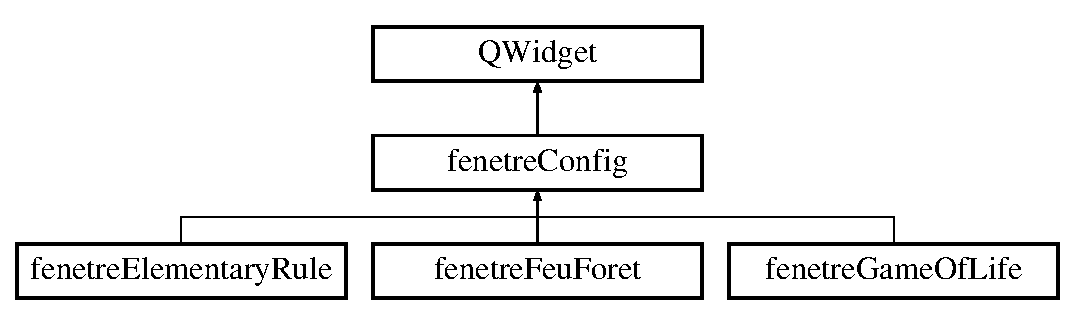
\includegraphics[height=3.000000cm]{classfenetre_config}
\end{center}
\end{figure}
\subsection*{Signaux}
\begin{DoxyCompactItemize}
\item 
void \mbox{\hyperlink{classfenetre_config_a9bec5e0d532367badb669f28eb3cad0d}{config\+Construite}} (int) const
\end{DoxyCompactItemize}
\subsection*{Fonctions membres publiques}
\begin{DoxyCompactItemize}
\item 
\mbox{\hyperlink{classfenetre_config_ac1515d010b54334e6a6bd121d5756f35}{fenetre\+Config}} (Q\+Widget $\ast$parent=nullptr)
\item 
virtual void \mbox{\hyperlink{classfenetre_config_a67e3561304b9c53dc01ae3f3b3713c11}{construction\+Automate}} () const =0
\item 
virtual \mbox{\hyperlink{classfenetre_config_a84bee3769f0b8e5b38bc1f09449689e1}{$\sim$fenetre\+Config}} ()
\item 
virtual void \mbox{\hyperlink{classfenetre_config_afab21d3c10c4b7779614da983e1e9bd5}{load\+Config}} ()=0
\item 
virtual void \mbox{\hyperlink{classfenetre_config_a4bdf35ea6efe26c3e9b1cea487931ba1}{save\+Config}} ()=0
\end{DoxyCompactItemize}


\subsection{Documentation des constructeurs et destructeur}
\mbox{\Hypertarget{classfenetre_config_ac1515d010b54334e6a6bd121d5756f35}\label{classfenetre_config_ac1515d010b54334e6a6bd121d5756f35}} 
\index{fenetre\+Config@{fenetre\+Config}!fenetre\+Config@{fenetre\+Config}}
\index{fenetre\+Config@{fenetre\+Config}!fenetre\+Config@{fenetre\+Config}}
\subsubsection{\texorpdfstring{fenetre\+Config()}{fenetreConfig()}}
{\footnotesize\ttfamily fenetre\+Config\+::fenetre\+Config (\begin{DoxyParamCaption}\item[{Q\+Widget $\ast$}]{parent = {\ttfamily nullptr} }\end{DoxyParamCaption})\hspace{0.3cm}{\ttfamily [inline]}, {\ttfamily [explicit]}}

\mbox{\Hypertarget{classfenetre_config_a84bee3769f0b8e5b38bc1f09449689e1}\label{classfenetre_config_a84bee3769f0b8e5b38bc1f09449689e1}} 
\index{fenetre\+Config@{fenetre\+Config}!````~fenetre\+Config@{$\sim$fenetre\+Config}}
\index{````~fenetre\+Config@{$\sim$fenetre\+Config}!fenetre\+Config@{fenetre\+Config}}
\subsubsection{\texorpdfstring{$\sim$fenetre\+Config()}{~fenetreConfig()}}
{\footnotesize\ttfamily virtual fenetre\+Config\+::$\sim$fenetre\+Config (\begin{DoxyParamCaption}{ }\end{DoxyParamCaption})\hspace{0.3cm}{\ttfamily [inline]}, {\ttfamily [virtual]}}



\subsection{Documentation des fonctions membres}
\mbox{\Hypertarget{classfenetre_config_a9bec5e0d532367badb669f28eb3cad0d}\label{classfenetre_config_a9bec5e0d532367badb669f28eb3cad0d}} 
\index{fenetre\+Config@{fenetre\+Config}!config\+Construite@{config\+Construite}}
\index{config\+Construite@{config\+Construite}!fenetre\+Config@{fenetre\+Config}}
\subsubsection{\texorpdfstring{config\+Construite}{configConstruite}}
{\footnotesize\ttfamily void fenetre\+Config\+::config\+Construite (\begin{DoxyParamCaption}\item[{int}]{ }\end{DoxyParamCaption}) const\hspace{0.3cm}{\ttfamily [signal]}}

\mbox{\Hypertarget{classfenetre_config_a67e3561304b9c53dc01ae3f3b3713c11}\label{classfenetre_config_a67e3561304b9c53dc01ae3f3b3713c11}} 
\index{fenetre\+Config@{fenetre\+Config}!construction\+Automate@{construction\+Automate}}
\index{construction\+Automate@{construction\+Automate}!fenetre\+Config@{fenetre\+Config}}
\subsubsection{\texorpdfstring{construction\+Automate()}{constructionAutomate()}}
{\footnotesize\ttfamily virtual void fenetre\+Config\+::construction\+Automate (\begin{DoxyParamCaption}{ }\end{DoxyParamCaption}) const\hspace{0.3cm}{\ttfamily [pure virtual]}}



Implémenté dans \mbox{\hyperlink{classfenetre_feu_foret_a41d2078bf781a32157d526f623a55b28}{fenetre\+Feu\+Foret}}, \mbox{\hyperlink{classfenetre_game_of_life_a76bc46f313a3d3b39ab060702de0b614}{fenetre\+Game\+Of\+Life}}, et \mbox{\hyperlink{classfenetre_elementary_rule_a37932a84243abfe789e6d18bdeb4324f}{fenetre\+Elementary\+Rule}}.

\mbox{\Hypertarget{classfenetre_config_afab21d3c10c4b7779614da983e1e9bd5}\label{classfenetre_config_afab21d3c10c4b7779614da983e1e9bd5}} 
\index{fenetre\+Config@{fenetre\+Config}!load\+Config@{load\+Config}}
\index{load\+Config@{load\+Config}!fenetre\+Config@{fenetre\+Config}}
\subsubsection{\texorpdfstring{load\+Config()}{loadConfig()}}
{\footnotesize\ttfamily virtual void fenetre\+Config\+::load\+Config (\begin{DoxyParamCaption}{ }\end{DoxyParamCaption})\hspace{0.3cm}{\ttfamily [pure virtual]}}



Implémenté dans \mbox{\hyperlink{classfenetre_feu_foret_a0a835b46bd202080341290a7fa784c4f}{fenetre\+Feu\+Foret}}, \mbox{\hyperlink{classfenetre_game_of_life_a336a5b5e63dcddc116cc7bfc96d21dd8}{fenetre\+Game\+Of\+Life}}, et \mbox{\hyperlink{classfenetre_elementary_rule_affa7e46edbb21d5ef745957aab91daab}{fenetre\+Elementary\+Rule}}.

\mbox{\Hypertarget{classfenetre_config_a4bdf35ea6efe26c3e9b1cea487931ba1}\label{classfenetre_config_a4bdf35ea6efe26c3e9b1cea487931ba1}} 
\index{fenetre\+Config@{fenetre\+Config}!save\+Config@{save\+Config}}
\index{save\+Config@{save\+Config}!fenetre\+Config@{fenetre\+Config}}
\subsubsection{\texorpdfstring{save\+Config()}{saveConfig()}}
{\footnotesize\ttfamily virtual void fenetre\+Config\+::save\+Config (\begin{DoxyParamCaption}{ }\end{DoxyParamCaption})\hspace{0.3cm}{\ttfamily [pure virtual]}}



Implémenté dans \mbox{\hyperlink{classfenetre_feu_foret_a50d73cad62240b54640048cb254ddf13}{fenetre\+Feu\+Foret}}, \mbox{\hyperlink{classfenetre_game_of_life_aaa79df41aba182775dab13d42656220a}{fenetre\+Game\+Of\+Life}}, et \mbox{\hyperlink{classfenetre_elementary_rule_a36f7a8541be65aa1488fe251b0a6d277}{fenetre\+Elementary\+Rule}}.



La documentation de cette classe a été générée à partir du fichier suivant \+:\begin{DoxyCompactItemize}
\item 
C\+:/\+Users/maxn0/git/\+L\+O21/\+Auto\+Cell/\mbox{\hyperlink{fenetreconfig_8h}{fenetreconfig.\+h}}\end{DoxyCompactItemize}

\hypertarget{classfenetre_elementary_rule}{}\section{Référence de la classe fenetre\+Elementary\+Rule}
\label{classfenetre_elementary_rule}\index{fenetre\+Elementary\+Rule@{fenetre\+Elementary\+Rule}}


{\ttfamily \#include $<$fenetreconfig.\+h$>$}

Graphe d\textquotesingle{}héritage de fenetre\+Elementary\+Rule\+:\begin{figure}[H]
\begin{center}
\leavevmode
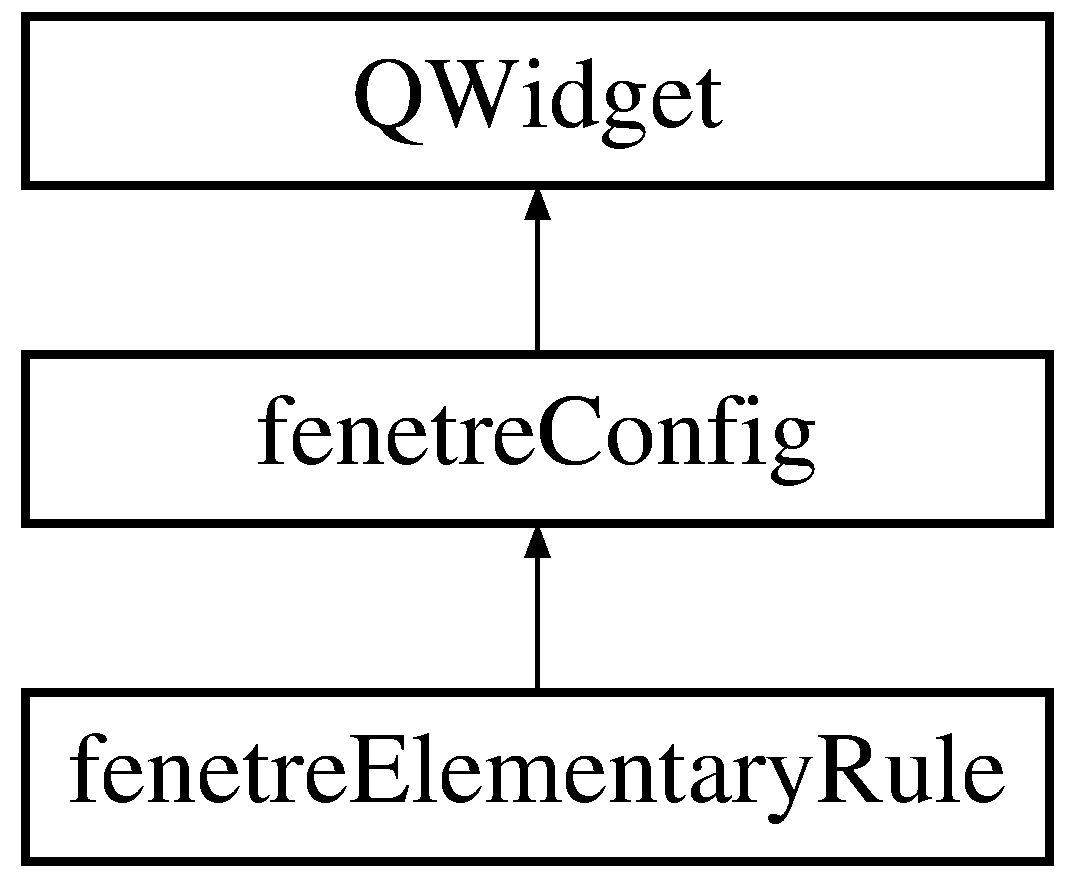
\includegraphics[height=3.000000cm]{classfenetre_elementary_rule}
\end{center}
\end{figure}
\subsection*{Fonctions membres publiques}
\begin{DoxyCompactItemize}
\item 
\mbox{\hyperlink{classfenetre_elementary_rule_a6230faa9586917afbe72a85555581da9}{fenetre\+Elementary\+Rule}} (Q\+Widget $\ast$parent=nullptr)
\item 
void \mbox{\hyperlink{classfenetre_elementary_rule_a37932a84243abfe789e6d18bdeb4324f}{construction\+Automate}} () const override
\item 
\mbox{\hyperlink{classfenetre_elementary_rule_a28139807cf1f5d842ca7fadf7df494f4}{$\sim$fenetre\+Elementary\+Rule}} ()
\item 
virtual void \mbox{\hyperlink{classfenetre_elementary_rule_affa7e46edbb21d5ef745957aab91daab}{load\+Config}} () override
\item 
virtual void \mbox{\hyperlink{classfenetre_elementary_rule_a36f7a8541be65aa1488fe251b0a6d277}{save\+Config}} () override
\end{DoxyCompactItemize}
\subsection*{Connecteurs privés}
\begin{DoxyCompactItemize}
\item 
void \mbox{\hyperlink{classfenetre_elementary_rule_ab662e4e95dd973b399b9fc0182f80c8c}{changement\+Reg\+Exp}} ()
\item 
void \mbox{\hyperlink{classfenetre_elementary_rule_a7f6fed3ef71ae9a0d2264477690d3908}{changement\+Label}} ()
\end{DoxyCompactItemize}
\subsection*{Attributs privés}
\begin{DoxyCompactItemize}
\item 
Q\+Spin\+Box $\ast$ \mbox{\hyperlink{classfenetre_elementary_rule_a2283bd95c86db69e65abd4939360d30a}{m\+\_\+nombre\+Etats}}
\item 
Q\+Line\+Edit $\ast$ \mbox{\hyperlink{classfenetre_elementary_rule_ac9e91c2d984c3ed4611deef053a702be}{m\+\_\+regle}}
\item 
Q\+Reg\+Exp\+Validator $\ast$ \mbox{\hyperlink{classfenetre_elementary_rule_a6a36eabf6f070882df6afe328debd6a4}{m\+\_\+regle\+Validator}}
\item 
Q\+Label $\ast$ \mbox{\hyperlink{classfenetre_elementary_rule_a34ced18693114e7bdd0030b26878e3c5}{nb\+Caract}}
\end{DoxyCompactItemize}
\subsection*{Attributs privés statiques}
\begin{DoxyCompactItemize}
\item 
static const unsigned int \mbox{\hyperlink{classfenetre_elementary_rule_aa60ec0fd673b59b9d52c70bea37f212f}{m\+\_\+ordre\+Voisinage}} = 1
\end{DoxyCompactItemize}
\subsection*{Membres hérités additionnels}


\subsection{Documentation des constructeurs et destructeur}
\mbox{\Hypertarget{classfenetre_elementary_rule_a6230faa9586917afbe72a85555581da9}\label{classfenetre_elementary_rule_a6230faa9586917afbe72a85555581da9}} 
\index{fenetre\+Elementary\+Rule@{fenetre\+Elementary\+Rule}!fenetre\+Elementary\+Rule@{fenetre\+Elementary\+Rule}}
\index{fenetre\+Elementary\+Rule@{fenetre\+Elementary\+Rule}!fenetre\+Elementary\+Rule@{fenetre\+Elementary\+Rule}}
\subsubsection{\texorpdfstring{fenetre\+Elementary\+Rule()}{fenetreElementaryRule()}}
{\footnotesize\ttfamily fenetre\+Elementary\+Rule\+::fenetre\+Elementary\+Rule (\begin{DoxyParamCaption}\item[{Q\+Widget $\ast$}]{parent = {\ttfamily nullptr} }\end{DoxyParamCaption})\hspace{0.3cm}{\ttfamily [explicit]}}

\mbox{\Hypertarget{classfenetre_elementary_rule_a28139807cf1f5d842ca7fadf7df494f4}\label{classfenetre_elementary_rule_a28139807cf1f5d842ca7fadf7df494f4}} 
\index{fenetre\+Elementary\+Rule@{fenetre\+Elementary\+Rule}!````~fenetre\+Elementary\+Rule@{$\sim$fenetre\+Elementary\+Rule}}
\index{````~fenetre\+Elementary\+Rule@{$\sim$fenetre\+Elementary\+Rule}!fenetre\+Elementary\+Rule@{fenetre\+Elementary\+Rule}}
\subsubsection{\texorpdfstring{$\sim$fenetre\+Elementary\+Rule()}{~fenetreElementaryRule()}}
{\footnotesize\ttfamily fenetre\+Elementary\+Rule\+::$\sim$fenetre\+Elementary\+Rule (\begin{DoxyParamCaption}{ }\end{DoxyParamCaption})\hspace{0.3cm}{\ttfamily [inline]}}



\subsection{Documentation des fonctions membres}
\mbox{\Hypertarget{classfenetre_elementary_rule_a7f6fed3ef71ae9a0d2264477690d3908}\label{classfenetre_elementary_rule_a7f6fed3ef71ae9a0d2264477690d3908}} 
\index{fenetre\+Elementary\+Rule@{fenetre\+Elementary\+Rule}!changement\+Label@{changement\+Label}}
\index{changement\+Label@{changement\+Label}!fenetre\+Elementary\+Rule@{fenetre\+Elementary\+Rule}}
\subsubsection{\texorpdfstring{changement\+Label}{changementLabel}}
{\footnotesize\ttfamily void fenetre\+Elementary\+Rule\+::changement\+Label (\begin{DoxyParamCaption}{ }\end{DoxyParamCaption})\hspace{0.3cm}{\ttfamily [private]}, {\ttfamily [slot]}}

\mbox{\Hypertarget{classfenetre_elementary_rule_ab662e4e95dd973b399b9fc0182f80c8c}\label{classfenetre_elementary_rule_ab662e4e95dd973b399b9fc0182f80c8c}} 
\index{fenetre\+Elementary\+Rule@{fenetre\+Elementary\+Rule}!changement\+Reg\+Exp@{changement\+Reg\+Exp}}
\index{changement\+Reg\+Exp@{changement\+Reg\+Exp}!fenetre\+Elementary\+Rule@{fenetre\+Elementary\+Rule}}
\subsubsection{\texorpdfstring{changement\+Reg\+Exp}{changementRegExp}}
{\footnotesize\ttfamily void fenetre\+Elementary\+Rule\+::changement\+Reg\+Exp (\begin{DoxyParamCaption}{ }\end{DoxyParamCaption})\hspace{0.3cm}{\ttfamily [private]}, {\ttfamily [slot]}}

\mbox{\Hypertarget{classfenetre_elementary_rule_a37932a84243abfe789e6d18bdeb4324f}\label{classfenetre_elementary_rule_a37932a84243abfe789e6d18bdeb4324f}} 
\index{fenetre\+Elementary\+Rule@{fenetre\+Elementary\+Rule}!construction\+Automate@{construction\+Automate}}
\index{construction\+Automate@{construction\+Automate}!fenetre\+Elementary\+Rule@{fenetre\+Elementary\+Rule}}
\subsubsection{\texorpdfstring{construction\+Automate()}{constructionAutomate()}}
{\footnotesize\ttfamily void fenetre\+Elementary\+Rule\+::construction\+Automate (\begin{DoxyParamCaption}{ }\end{DoxyParamCaption}) const\hspace{0.3cm}{\ttfamily [override]}, {\ttfamily [virtual]}}



Implémente \mbox{\hyperlink{classfenetre_config_a67e3561304b9c53dc01ae3f3b3713c11}{fenetre\+Config}}.

\mbox{\Hypertarget{classfenetre_elementary_rule_affa7e46edbb21d5ef745957aab91daab}\label{classfenetre_elementary_rule_affa7e46edbb21d5ef745957aab91daab}} 
\index{fenetre\+Elementary\+Rule@{fenetre\+Elementary\+Rule}!load\+Config@{load\+Config}}
\index{load\+Config@{load\+Config}!fenetre\+Elementary\+Rule@{fenetre\+Elementary\+Rule}}
\subsubsection{\texorpdfstring{load\+Config()}{loadConfig()}}
{\footnotesize\ttfamily void fenetre\+Elementary\+Rule\+::load\+Config (\begin{DoxyParamCaption}{ }\end{DoxyParamCaption})\hspace{0.3cm}{\ttfamily [override]}, {\ttfamily [virtual]}}



Implémente \mbox{\hyperlink{classfenetre_config_afab21d3c10c4b7779614da983e1e9bd5}{fenetre\+Config}}.

\mbox{\Hypertarget{classfenetre_elementary_rule_a36f7a8541be65aa1488fe251b0a6d277}\label{classfenetre_elementary_rule_a36f7a8541be65aa1488fe251b0a6d277}} 
\index{fenetre\+Elementary\+Rule@{fenetre\+Elementary\+Rule}!save\+Config@{save\+Config}}
\index{save\+Config@{save\+Config}!fenetre\+Elementary\+Rule@{fenetre\+Elementary\+Rule}}
\subsubsection{\texorpdfstring{save\+Config()}{saveConfig()}}
{\footnotesize\ttfamily void fenetre\+Elementary\+Rule\+::save\+Config (\begin{DoxyParamCaption}{ }\end{DoxyParamCaption})\hspace{0.3cm}{\ttfamily [override]}, {\ttfamily [virtual]}}



Implémente \mbox{\hyperlink{classfenetre_config_a4bdf35ea6efe26c3e9b1cea487931ba1}{fenetre\+Config}}.



\subsection{Documentation des données membres}
\mbox{\Hypertarget{classfenetre_elementary_rule_a2283bd95c86db69e65abd4939360d30a}\label{classfenetre_elementary_rule_a2283bd95c86db69e65abd4939360d30a}} 
\index{fenetre\+Elementary\+Rule@{fenetre\+Elementary\+Rule}!m\+\_\+nombre\+Etats@{m\+\_\+nombre\+Etats}}
\index{m\+\_\+nombre\+Etats@{m\+\_\+nombre\+Etats}!fenetre\+Elementary\+Rule@{fenetre\+Elementary\+Rule}}
\subsubsection{\texorpdfstring{m\+\_\+nombre\+Etats}{m\_nombreEtats}}
{\footnotesize\ttfamily Q\+Spin\+Box$\ast$ fenetre\+Elementary\+Rule\+::m\+\_\+nombre\+Etats\hspace{0.3cm}{\ttfamily [private]}}

\mbox{\Hypertarget{classfenetre_elementary_rule_aa60ec0fd673b59b9d52c70bea37f212f}\label{classfenetre_elementary_rule_aa60ec0fd673b59b9d52c70bea37f212f}} 
\index{fenetre\+Elementary\+Rule@{fenetre\+Elementary\+Rule}!m\+\_\+ordre\+Voisinage@{m\+\_\+ordre\+Voisinage}}
\index{m\+\_\+ordre\+Voisinage@{m\+\_\+ordre\+Voisinage}!fenetre\+Elementary\+Rule@{fenetre\+Elementary\+Rule}}
\subsubsection{\texorpdfstring{m\+\_\+ordre\+Voisinage}{m\_ordreVoisinage}}
{\footnotesize\ttfamily const unsigned int fenetre\+Elementary\+Rule\+::m\+\_\+ordre\+Voisinage = 1\hspace{0.3cm}{\ttfamily [static]}, {\ttfamily [private]}}

\mbox{\Hypertarget{classfenetre_elementary_rule_ac9e91c2d984c3ed4611deef053a702be}\label{classfenetre_elementary_rule_ac9e91c2d984c3ed4611deef053a702be}} 
\index{fenetre\+Elementary\+Rule@{fenetre\+Elementary\+Rule}!m\+\_\+regle@{m\+\_\+regle}}
\index{m\+\_\+regle@{m\+\_\+regle}!fenetre\+Elementary\+Rule@{fenetre\+Elementary\+Rule}}
\subsubsection{\texorpdfstring{m\+\_\+regle}{m\_regle}}
{\footnotesize\ttfamily Q\+Line\+Edit$\ast$ fenetre\+Elementary\+Rule\+::m\+\_\+regle\hspace{0.3cm}{\ttfamily [private]}}

\mbox{\Hypertarget{classfenetre_elementary_rule_a6a36eabf6f070882df6afe328debd6a4}\label{classfenetre_elementary_rule_a6a36eabf6f070882df6afe328debd6a4}} 
\index{fenetre\+Elementary\+Rule@{fenetre\+Elementary\+Rule}!m\+\_\+regle\+Validator@{m\+\_\+regle\+Validator}}
\index{m\+\_\+regle\+Validator@{m\+\_\+regle\+Validator}!fenetre\+Elementary\+Rule@{fenetre\+Elementary\+Rule}}
\subsubsection{\texorpdfstring{m\+\_\+regle\+Validator}{m\_regleValidator}}
{\footnotesize\ttfamily Q\+Reg\+Exp\+Validator$\ast$ fenetre\+Elementary\+Rule\+::m\+\_\+regle\+Validator\hspace{0.3cm}{\ttfamily [private]}}

\mbox{\Hypertarget{classfenetre_elementary_rule_a34ced18693114e7bdd0030b26878e3c5}\label{classfenetre_elementary_rule_a34ced18693114e7bdd0030b26878e3c5}} 
\index{fenetre\+Elementary\+Rule@{fenetre\+Elementary\+Rule}!nb\+Caract@{nb\+Caract}}
\index{nb\+Caract@{nb\+Caract}!fenetre\+Elementary\+Rule@{fenetre\+Elementary\+Rule}}
\subsubsection{\texorpdfstring{nb\+Caract}{nbCaract}}
{\footnotesize\ttfamily Q\+Label$\ast$ fenetre\+Elementary\+Rule\+::nb\+Caract\hspace{0.3cm}{\ttfamily [private]}}



La documentation de cette classe a été générée à partir des fichiers suivants \+:\begin{DoxyCompactItemize}
\item 
C\+:/\+Users/maxn0/git/\+L\+O21/\+Auto\+Cell/\mbox{\hyperlink{fenetreconfig_8h}{fenetreconfig.\+h}}\item 
C\+:/\+Users/maxn0/git/\+L\+O21/\+Auto\+Cell/\mbox{\hyperlink{fenetreconfig_8cpp}{fenetreconfig.\+cpp}}\end{DoxyCompactItemize}

\hypertarget{classfenetre_feu_foret}{}\section{Référence de la classe fenetre\+Feu\+Foret}
\label{classfenetre_feu_foret}\index{fenetre\+Feu\+Foret@{fenetre\+Feu\+Foret}}


{\ttfamily \#include $<$fenetreconfig.\+h$>$}

Graphe d\textquotesingle{}héritage de fenetre\+Feu\+Foret\+:\begin{figure}[H]
\begin{center}
\leavevmode
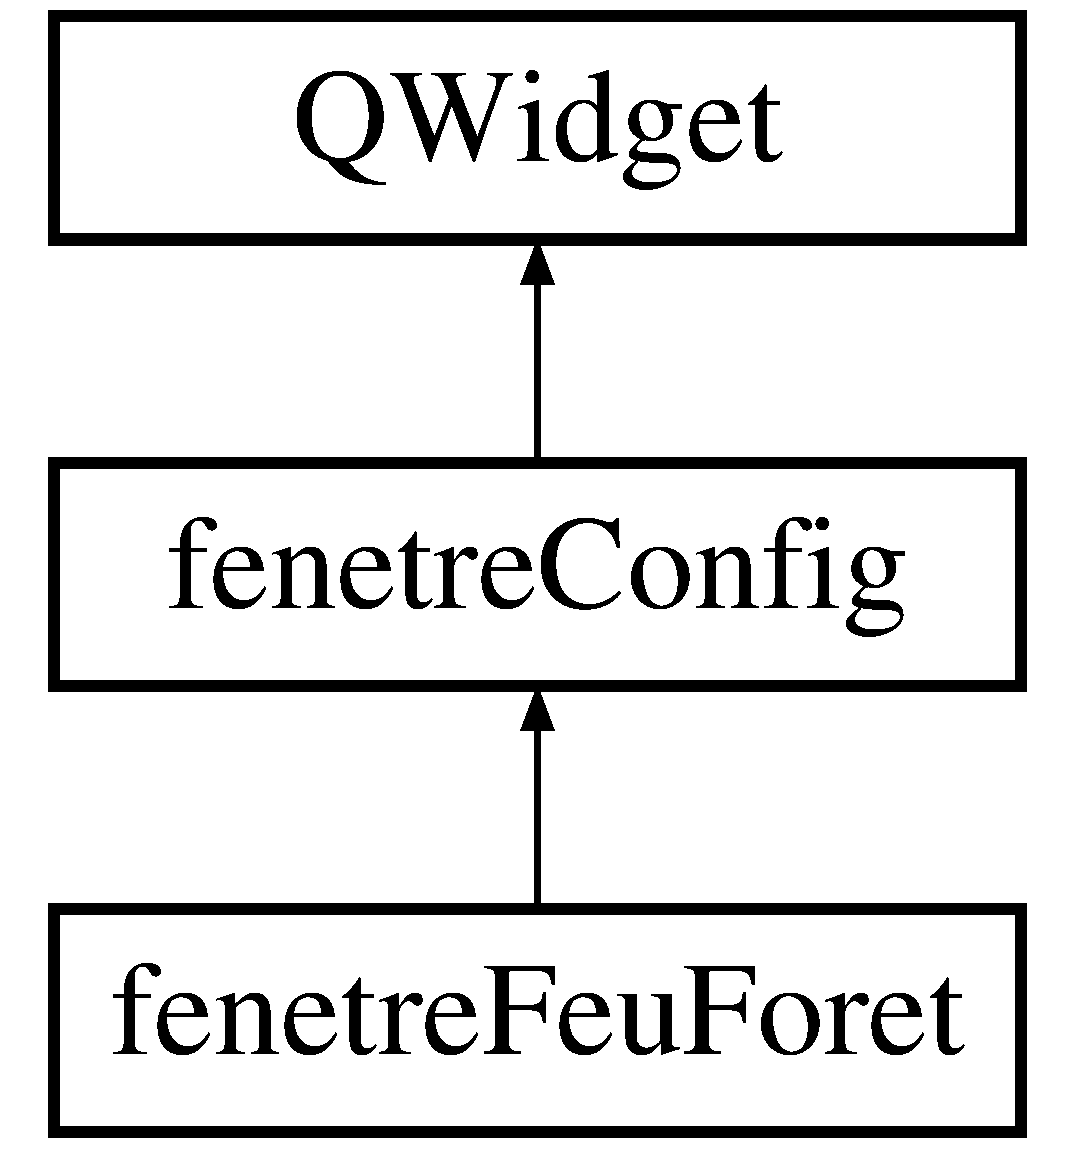
\includegraphics[height=3.000000cm]{classfenetre_feu_foret}
\end{center}
\end{figure}
\subsection*{Fonctions membres publiques}
\begin{DoxyCompactItemize}
\item 
\mbox{\hyperlink{classfenetre_feu_foret_a31576258d5cd4214d9a04d0735db5a70}{fenetre\+Feu\+Foret}} (Q\+Widget $\ast$parent=nullptr)
\item 
void \mbox{\hyperlink{classfenetre_feu_foret_a41d2078bf781a32157d526f623a55b28}{construction\+Automate}} () const override
\item 
\mbox{\hyperlink{classfenetre_feu_foret_a0dcccc1dc84cb39e97c50933265785c2}{$\sim$fenetre\+Feu\+Foret}} ()
\item 
virtual void \mbox{\hyperlink{classfenetre_feu_foret_a0a835b46bd202080341290a7fa784c4f}{load\+Config}} () override
\item 
virtual void \mbox{\hyperlink{classfenetre_feu_foret_a50d73cad62240b54640048cb254ddf13}{save\+Config}} () override
\end{DoxyCompactItemize}
\subsection*{Attributs privés}
\begin{DoxyCompactItemize}
\item 
Q\+Combo\+Box $\ast$ \mbox{\hyperlink{classfenetre_feu_foret_ac8c9731bc5722f246bda69ba593f7540}{m\+\_\+choix\+Voisinage}}
\item 
Q\+Spin\+Box $\ast$ \mbox{\hyperlink{classfenetre_feu_foret_a9be2039cf42d85e672b8505f60a53629}{m\+\_\+ordre\+Voisinage}}
\end{DoxyCompactItemize}
\subsection*{Attributs privés statiques}
\begin{DoxyCompactItemize}
\item 
static const unsigned int \mbox{\hyperlink{classfenetre_feu_foret_a5dc92976b1fd63f7e23be877c2904947}{m\+\_\+nombre\+Etats}} = 4
\end{DoxyCompactItemize}
\subsection*{Membres hérités additionnels}


\subsection{Documentation des constructeurs et destructeur}
\mbox{\Hypertarget{classfenetre_feu_foret_a31576258d5cd4214d9a04d0735db5a70}\label{classfenetre_feu_foret_a31576258d5cd4214d9a04d0735db5a70}} 
\index{fenetre\+Feu\+Foret@{fenetre\+Feu\+Foret}!fenetre\+Feu\+Foret@{fenetre\+Feu\+Foret}}
\index{fenetre\+Feu\+Foret@{fenetre\+Feu\+Foret}!fenetre\+Feu\+Foret@{fenetre\+Feu\+Foret}}
\subsubsection{\texorpdfstring{fenetre\+Feu\+Foret()}{fenetreFeuForet()}}
{\footnotesize\ttfamily fenetre\+Feu\+Foret\+::fenetre\+Feu\+Foret (\begin{DoxyParamCaption}\item[{Q\+Widget $\ast$}]{parent = {\ttfamily nullptr} }\end{DoxyParamCaption})\hspace{0.3cm}{\ttfamily [explicit]}}

\mbox{\Hypertarget{classfenetre_feu_foret_a0dcccc1dc84cb39e97c50933265785c2}\label{classfenetre_feu_foret_a0dcccc1dc84cb39e97c50933265785c2}} 
\index{fenetre\+Feu\+Foret@{fenetre\+Feu\+Foret}!````~fenetre\+Feu\+Foret@{$\sim$fenetre\+Feu\+Foret}}
\index{````~fenetre\+Feu\+Foret@{$\sim$fenetre\+Feu\+Foret}!fenetre\+Feu\+Foret@{fenetre\+Feu\+Foret}}
\subsubsection{\texorpdfstring{$\sim$fenetre\+Feu\+Foret()}{~fenetreFeuForet()}}
{\footnotesize\ttfamily fenetre\+Feu\+Foret\+::$\sim$fenetre\+Feu\+Foret (\begin{DoxyParamCaption}{ }\end{DoxyParamCaption})\hspace{0.3cm}{\ttfamily [inline]}}



\subsection{Documentation des fonctions membres}
\mbox{\Hypertarget{classfenetre_feu_foret_a41d2078bf781a32157d526f623a55b28}\label{classfenetre_feu_foret_a41d2078bf781a32157d526f623a55b28}} 
\index{fenetre\+Feu\+Foret@{fenetre\+Feu\+Foret}!construction\+Automate@{construction\+Automate}}
\index{construction\+Automate@{construction\+Automate}!fenetre\+Feu\+Foret@{fenetre\+Feu\+Foret}}
\subsubsection{\texorpdfstring{construction\+Automate()}{constructionAutomate()}}
{\footnotesize\ttfamily void fenetre\+Feu\+Foret\+::construction\+Automate (\begin{DoxyParamCaption}{ }\end{DoxyParamCaption}) const\hspace{0.3cm}{\ttfamily [override]}, {\ttfamily [virtual]}}



Implémente \mbox{\hyperlink{classfenetre_config_a67e3561304b9c53dc01ae3f3b3713c11}{fenetre\+Config}}.

\mbox{\Hypertarget{classfenetre_feu_foret_a0a835b46bd202080341290a7fa784c4f}\label{classfenetre_feu_foret_a0a835b46bd202080341290a7fa784c4f}} 
\index{fenetre\+Feu\+Foret@{fenetre\+Feu\+Foret}!load\+Config@{load\+Config}}
\index{load\+Config@{load\+Config}!fenetre\+Feu\+Foret@{fenetre\+Feu\+Foret}}
\subsubsection{\texorpdfstring{load\+Config()}{loadConfig()}}
{\footnotesize\ttfamily void fenetre\+Feu\+Foret\+::load\+Config (\begin{DoxyParamCaption}{ }\end{DoxyParamCaption})\hspace{0.3cm}{\ttfamily [override]}, {\ttfamily [virtual]}}



Implémente \mbox{\hyperlink{classfenetre_config_afab21d3c10c4b7779614da983e1e9bd5}{fenetre\+Config}}.

\mbox{\Hypertarget{classfenetre_feu_foret_a50d73cad62240b54640048cb254ddf13}\label{classfenetre_feu_foret_a50d73cad62240b54640048cb254ddf13}} 
\index{fenetre\+Feu\+Foret@{fenetre\+Feu\+Foret}!save\+Config@{save\+Config}}
\index{save\+Config@{save\+Config}!fenetre\+Feu\+Foret@{fenetre\+Feu\+Foret}}
\subsubsection{\texorpdfstring{save\+Config()}{saveConfig()}}
{\footnotesize\ttfamily void fenetre\+Feu\+Foret\+::save\+Config (\begin{DoxyParamCaption}{ }\end{DoxyParamCaption})\hspace{0.3cm}{\ttfamily [override]}, {\ttfamily [virtual]}}



Implémente \mbox{\hyperlink{classfenetre_config_a4bdf35ea6efe26c3e9b1cea487931ba1}{fenetre\+Config}}.



\subsection{Documentation des données membres}
\mbox{\Hypertarget{classfenetre_feu_foret_ac8c9731bc5722f246bda69ba593f7540}\label{classfenetre_feu_foret_ac8c9731bc5722f246bda69ba593f7540}} 
\index{fenetre\+Feu\+Foret@{fenetre\+Feu\+Foret}!m\+\_\+choix\+Voisinage@{m\+\_\+choix\+Voisinage}}
\index{m\+\_\+choix\+Voisinage@{m\+\_\+choix\+Voisinage}!fenetre\+Feu\+Foret@{fenetre\+Feu\+Foret}}
\subsubsection{\texorpdfstring{m\+\_\+choix\+Voisinage}{m\_choixVoisinage}}
{\footnotesize\ttfamily Q\+Combo\+Box$\ast$ fenetre\+Feu\+Foret\+::m\+\_\+choix\+Voisinage\hspace{0.3cm}{\ttfamily [private]}}

\mbox{\Hypertarget{classfenetre_feu_foret_a5dc92976b1fd63f7e23be877c2904947}\label{classfenetre_feu_foret_a5dc92976b1fd63f7e23be877c2904947}} 
\index{fenetre\+Feu\+Foret@{fenetre\+Feu\+Foret}!m\+\_\+nombre\+Etats@{m\+\_\+nombre\+Etats}}
\index{m\+\_\+nombre\+Etats@{m\+\_\+nombre\+Etats}!fenetre\+Feu\+Foret@{fenetre\+Feu\+Foret}}
\subsubsection{\texorpdfstring{m\+\_\+nombre\+Etats}{m\_nombreEtats}}
{\footnotesize\ttfamily const unsigned int fenetre\+Feu\+Foret\+::m\+\_\+nombre\+Etats = 4\hspace{0.3cm}{\ttfamily [static]}, {\ttfamily [private]}}

\mbox{\Hypertarget{classfenetre_feu_foret_a9be2039cf42d85e672b8505f60a53629}\label{classfenetre_feu_foret_a9be2039cf42d85e672b8505f60a53629}} 
\index{fenetre\+Feu\+Foret@{fenetre\+Feu\+Foret}!m\+\_\+ordre\+Voisinage@{m\+\_\+ordre\+Voisinage}}
\index{m\+\_\+ordre\+Voisinage@{m\+\_\+ordre\+Voisinage}!fenetre\+Feu\+Foret@{fenetre\+Feu\+Foret}}
\subsubsection{\texorpdfstring{m\+\_\+ordre\+Voisinage}{m\_ordreVoisinage}}
{\footnotesize\ttfamily Q\+Spin\+Box$\ast$ fenetre\+Feu\+Foret\+::m\+\_\+ordre\+Voisinage\hspace{0.3cm}{\ttfamily [private]}}



La documentation de cette classe a été générée à partir des fichiers suivants \+:\begin{DoxyCompactItemize}
\item 
C\+:/\+Users/maxn0/git/\+L\+O21/\+Auto\+Cell/\mbox{\hyperlink{fenetreconfig_8h}{fenetreconfig.\+h}}\item 
C\+:/\+Users/maxn0/git/\+L\+O21/\+Auto\+Cell/\mbox{\hyperlink{fenetreconfig_8cpp}{fenetreconfig.\+cpp}}\end{DoxyCompactItemize}

\hypertarget{classfenetre_game_of_life}{}\section{Référence de la classe fenetre\+Game\+Of\+Life}
\label{classfenetre_game_of_life}\index{fenetre\+Game\+Of\+Life@{fenetre\+Game\+Of\+Life}}


{\ttfamily \#include $<$fenetreconfig.\+h$>$}

Graphe d\textquotesingle{}héritage de fenetre\+Game\+Of\+Life\+:\begin{figure}[H]
\begin{center}
\leavevmode
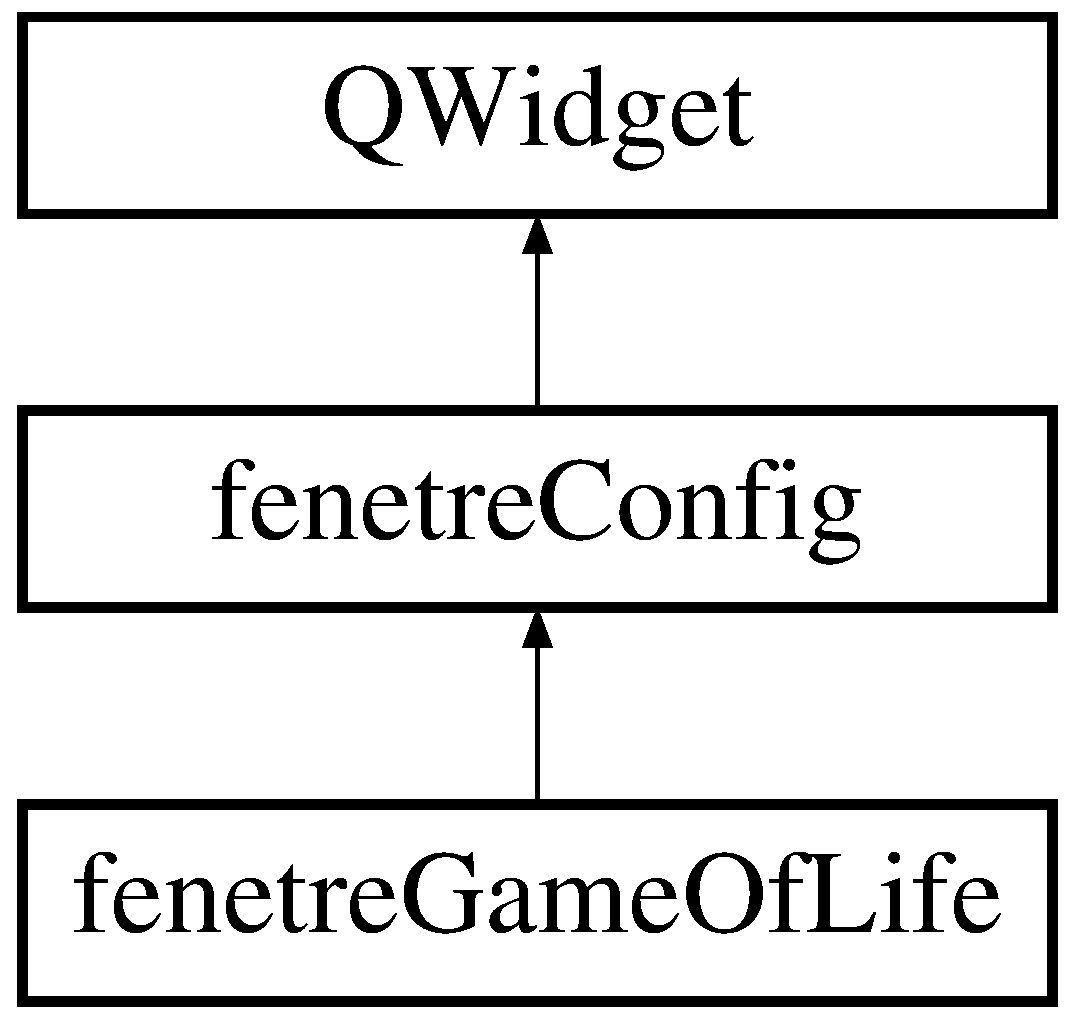
\includegraphics[height=3.000000cm]{classfenetre_game_of_life}
\end{center}
\end{figure}
\subsection*{Fonctions membres publiques}
\begin{DoxyCompactItemize}
\item 
\mbox{\hyperlink{classfenetre_game_of_life_a11bd76b5574d5bb2e0f1bb8114fab99f}{fenetre\+Game\+Of\+Life}} (Q\+Widget $\ast$parent=nullptr)
\item 
void \mbox{\hyperlink{classfenetre_game_of_life_a76bc46f313a3d3b39ab060702de0b614}{construction\+Automate}} () const override
\item 
\mbox{\hyperlink{classfenetre_game_of_life_a1cd09ff95e56f1b66b8a7a7f71fb44f2}{$\sim$fenetre\+Game\+Of\+Life}} ()
\item 
virtual void \mbox{\hyperlink{classfenetre_game_of_life_a336a5b5e63dcddc116cc7bfc96d21dd8}{load\+Config}} () override
\item 
virtual void \mbox{\hyperlink{classfenetre_game_of_life_aaa79df41aba182775dab13d42656220a}{save\+Config}} () override
\end{DoxyCompactItemize}
\subsection*{Attributs privés}
\begin{DoxyCompactItemize}
\item 
Q\+Combo\+Box $\ast$ \mbox{\hyperlink{classfenetre_game_of_life_a551b8c697797121124666e4917fa2df9}{m\+\_\+choix\+Voisinage}}
\item 
Q\+Spin\+Box $\ast$ \mbox{\hyperlink{classfenetre_game_of_life_a7267e755bb11b6949a049df4198f6a11}{m\+\_\+ordre\+Voisinage}}
\item 
Q\+Spin\+Box $\ast$ \mbox{\hyperlink{classfenetre_game_of_life_a54ed3c46d8409c0ec0f23a7b4aed11b0}{m\+\_\+min\+Vivants}}
\item 
Q\+Spin\+Box $\ast$ \mbox{\hyperlink{classfenetre_game_of_life_adfa79f81d5d2731529e046b338f4a481}{m\+\_\+max\+Vivants}}
\end{DoxyCompactItemize}
\subsection*{Attributs privés statiques}
\begin{DoxyCompactItemize}
\item 
static const unsigned int \mbox{\hyperlink{classfenetre_game_of_life_a979b46087690c0ba75798fb3d3db7acf}{m\+\_\+nombre\+Etats}} = 2
\end{DoxyCompactItemize}
\subsection*{Membres hérités additionnels}


\subsection{Documentation des constructeurs et destructeur}
\mbox{\Hypertarget{classfenetre_game_of_life_a11bd76b5574d5bb2e0f1bb8114fab99f}\label{classfenetre_game_of_life_a11bd76b5574d5bb2e0f1bb8114fab99f}} 
\index{fenetre\+Game\+Of\+Life@{fenetre\+Game\+Of\+Life}!fenetre\+Game\+Of\+Life@{fenetre\+Game\+Of\+Life}}
\index{fenetre\+Game\+Of\+Life@{fenetre\+Game\+Of\+Life}!fenetre\+Game\+Of\+Life@{fenetre\+Game\+Of\+Life}}
\subsubsection{\texorpdfstring{fenetre\+Game\+Of\+Life()}{fenetreGameOfLife()}}
{\footnotesize\ttfamily fenetre\+Game\+Of\+Life\+::fenetre\+Game\+Of\+Life (\begin{DoxyParamCaption}\item[{Q\+Widget $\ast$}]{parent = {\ttfamily nullptr} }\end{DoxyParamCaption})\hspace{0.3cm}{\ttfamily [explicit]}}

\mbox{\Hypertarget{classfenetre_game_of_life_a1cd09ff95e56f1b66b8a7a7f71fb44f2}\label{classfenetre_game_of_life_a1cd09ff95e56f1b66b8a7a7f71fb44f2}} 
\index{fenetre\+Game\+Of\+Life@{fenetre\+Game\+Of\+Life}!````~fenetre\+Game\+Of\+Life@{$\sim$fenetre\+Game\+Of\+Life}}
\index{````~fenetre\+Game\+Of\+Life@{$\sim$fenetre\+Game\+Of\+Life}!fenetre\+Game\+Of\+Life@{fenetre\+Game\+Of\+Life}}
\subsubsection{\texorpdfstring{$\sim$fenetre\+Game\+Of\+Life()}{~fenetreGameOfLife()}}
{\footnotesize\ttfamily fenetre\+Game\+Of\+Life\+::$\sim$fenetre\+Game\+Of\+Life (\begin{DoxyParamCaption}{ }\end{DoxyParamCaption})\hspace{0.3cm}{\ttfamily [inline]}}



\subsection{Documentation des fonctions membres}
\mbox{\Hypertarget{classfenetre_game_of_life_a76bc46f313a3d3b39ab060702de0b614}\label{classfenetre_game_of_life_a76bc46f313a3d3b39ab060702de0b614}} 
\index{fenetre\+Game\+Of\+Life@{fenetre\+Game\+Of\+Life}!construction\+Automate@{construction\+Automate}}
\index{construction\+Automate@{construction\+Automate}!fenetre\+Game\+Of\+Life@{fenetre\+Game\+Of\+Life}}
\subsubsection{\texorpdfstring{construction\+Automate()}{constructionAutomate()}}
{\footnotesize\ttfamily void fenetre\+Game\+Of\+Life\+::construction\+Automate (\begin{DoxyParamCaption}{ }\end{DoxyParamCaption}) const\hspace{0.3cm}{\ttfamily [override]}, {\ttfamily [virtual]}}



Implémente \mbox{\hyperlink{classfenetre_config_a67e3561304b9c53dc01ae3f3b3713c11}{fenetre\+Config}}.

\mbox{\Hypertarget{classfenetre_game_of_life_a336a5b5e63dcddc116cc7bfc96d21dd8}\label{classfenetre_game_of_life_a336a5b5e63dcddc116cc7bfc96d21dd8}} 
\index{fenetre\+Game\+Of\+Life@{fenetre\+Game\+Of\+Life}!load\+Config@{load\+Config}}
\index{load\+Config@{load\+Config}!fenetre\+Game\+Of\+Life@{fenetre\+Game\+Of\+Life}}
\subsubsection{\texorpdfstring{load\+Config()}{loadConfig()}}
{\footnotesize\ttfamily void fenetre\+Game\+Of\+Life\+::load\+Config (\begin{DoxyParamCaption}{ }\end{DoxyParamCaption})\hspace{0.3cm}{\ttfamily [override]}, {\ttfamily [virtual]}}



Implémente \mbox{\hyperlink{classfenetre_config_afab21d3c10c4b7779614da983e1e9bd5}{fenetre\+Config}}.

\mbox{\Hypertarget{classfenetre_game_of_life_aaa79df41aba182775dab13d42656220a}\label{classfenetre_game_of_life_aaa79df41aba182775dab13d42656220a}} 
\index{fenetre\+Game\+Of\+Life@{fenetre\+Game\+Of\+Life}!save\+Config@{save\+Config}}
\index{save\+Config@{save\+Config}!fenetre\+Game\+Of\+Life@{fenetre\+Game\+Of\+Life}}
\subsubsection{\texorpdfstring{save\+Config()}{saveConfig()}}
{\footnotesize\ttfamily void fenetre\+Game\+Of\+Life\+::save\+Config (\begin{DoxyParamCaption}{ }\end{DoxyParamCaption})\hspace{0.3cm}{\ttfamily [override]}, {\ttfamily [virtual]}}



Implémente \mbox{\hyperlink{classfenetre_config_a4bdf35ea6efe26c3e9b1cea487931ba1}{fenetre\+Config}}.



\subsection{Documentation des données membres}
\mbox{\Hypertarget{classfenetre_game_of_life_a551b8c697797121124666e4917fa2df9}\label{classfenetre_game_of_life_a551b8c697797121124666e4917fa2df9}} 
\index{fenetre\+Game\+Of\+Life@{fenetre\+Game\+Of\+Life}!m\+\_\+choix\+Voisinage@{m\+\_\+choix\+Voisinage}}
\index{m\+\_\+choix\+Voisinage@{m\+\_\+choix\+Voisinage}!fenetre\+Game\+Of\+Life@{fenetre\+Game\+Of\+Life}}
\subsubsection{\texorpdfstring{m\+\_\+choix\+Voisinage}{m\_choixVoisinage}}
{\footnotesize\ttfamily Q\+Combo\+Box$\ast$ fenetre\+Game\+Of\+Life\+::m\+\_\+choix\+Voisinage\hspace{0.3cm}{\ttfamily [private]}}

\mbox{\Hypertarget{classfenetre_game_of_life_adfa79f81d5d2731529e046b338f4a481}\label{classfenetre_game_of_life_adfa79f81d5d2731529e046b338f4a481}} 
\index{fenetre\+Game\+Of\+Life@{fenetre\+Game\+Of\+Life}!m\+\_\+max\+Vivants@{m\+\_\+max\+Vivants}}
\index{m\+\_\+max\+Vivants@{m\+\_\+max\+Vivants}!fenetre\+Game\+Of\+Life@{fenetre\+Game\+Of\+Life}}
\subsubsection{\texorpdfstring{m\+\_\+max\+Vivants}{m\_maxVivants}}
{\footnotesize\ttfamily Q\+Spin\+Box$\ast$ fenetre\+Game\+Of\+Life\+::m\+\_\+max\+Vivants\hspace{0.3cm}{\ttfamily [private]}}

\mbox{\Hypertarget{classfenetre_game_of_life_a54ed3c46d8409c0ec0f23a7b4aed11b0}\label{classfenetre_game_of_life_a54ed3c46d8409c0ec0f23a7b4aed11b0}} 
\index{fenetre\+Game\+Of\+Life@{fenetre\+Game\+Of\+Life}!m\+\_\+min\+Vivants@{m\+\_\+min\+Vivants}}
\index{m\+\_\+min\+Vivants@{m\+\_\+min\+Vivants}!fenetre\+Game\+Of\+Life@{fenetre\+Game\+Of\+Life}}
\subsubsection{\texorpdfstring{m\+\_\+min\+Vivants}{m\_minVivants}}
{\footnotesize\ttfamily Q\+Spin\+Box$\ast$ fenetre\+Game\+Of\+Life\+::m\+\_\+min\+Vivants\hspace{0.3cm}{\ttfamily [private]}}

\mbox{\Hypertarget{classfenetre_game_of_life_a979b46087690c0ba75798fb3d3db7acf}\label{classfenetre_game_of_life_a979b46087690c0ba75798fb3d3db7acf}} 
\index{fenetre\+Game\+Of\+Life@{fenetre\+Game\+Of\+Life}!m\+\_\+nombre\+Etats@{m\+\_\+nombre\+Etats}}
\index{m\+\_\+nombre\+Etats@{m\+\_\+nombre\+Etats}!fenetre\+Game\+Of\+Life@{fenetre\+Game\+Of\+Life}}
\subsubsection{\texorpdfstring{m\+\_\+nombre\+Etats}{m\_nombreEtats}}
{\footnotesize\ttfamily const unsigned int fenetre\+Game\+Of\+Life\+::m\+\_\+nombre\+Etats = 2\hspace{0.3cm}{\ttfamily [static]}, {\ttfamily [private]}}

\mbox{\Hypertarget{classfenetre_game_of_life_a7267e755bb11b6949a049df4198f6a11}\label{classfenetre_game_of_life_a7267e755bb11b6949a049df4198f6a11}} 
\index{fenetre\+Game\+Of\+Life@{fenetre\+Game\+Of\+Life}!m\+\_\+ordre\+Voisinage@{m\+\_\+ordre\+Voisinage}}
\index{m\+\_\+ordre\+Voisinage@{m\+\_\+ordre\+Voisinage}!fenetre\+Game\+Of\+Life@{fenetre\+Game\+Of\+Life}}
\subsubsection{\texorpdfstring{m\+\_\+ordre\+Voisinage}{m\_ordreVoisinage}}
{\footnotesize\ttfamily Q\+Spin\+Box$\ast$ fenetre\+Game\+Of\+Life\+::m\+\_\+ordre\+Voisinage\hspace{0.3cm}{\ttfamily [private]}}



La documentation de cette classe a été générée à partir des fichiers suivants \+:\begin{DoxyCompactItemize}
\item 
C\+:/\+Users/maxn0/git/\+L\+O21/\+Auto\+Cell/\mbox{\hyperlink{fenetreconfig_8h}{fenetreconfig.\+h}}\item 
C\+:/\+Users/maxn0/git/\+L\+O21/\+Auto\+Cell/\mbox{\hyperlink{fenetreconfig_8cpp}{fenetreconfig.\+cpp}}\end{DoxyCompactItemize}

\hypertarget{class_feu_foret}{}\section{Feu\+Foret Class Reference}
\label{class_feu_foret}\index{Feu\+Foret@{Feu\+Foret}}
Inheritance diagram for Feu\+Foret\+:\begin{figure}[H]
\begin{center}
\leavevmode
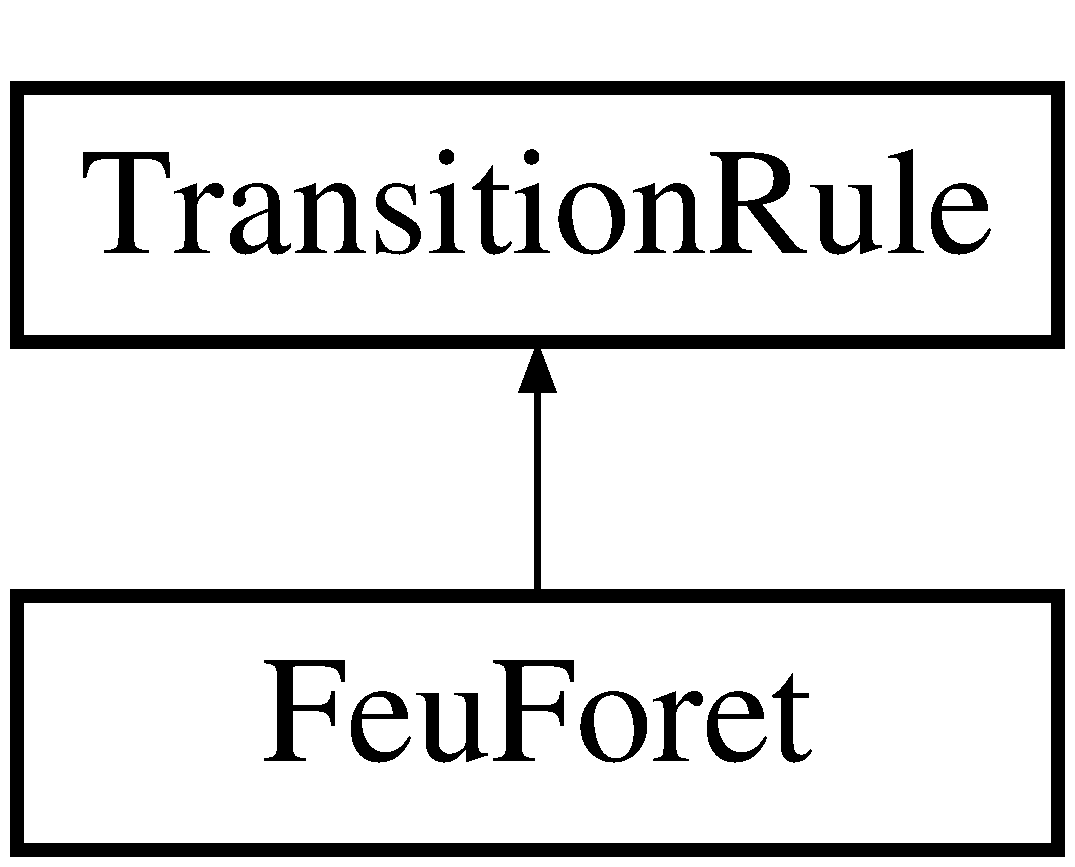
\includegraphics[height=3.000000cm]{class_feu_foret}
\end{center}
\end{figure}
\subsection*{Public Member Functions}
\begin{DoxyCompactItemize}
\item 
\mbox{\Hypertarget{class_feu_foret_a1fb3642690cc586faf0cbc6e9fae64cf}\label{class_feu_foret_a1fb3642690cc586faf0cbc6e9fae64cf}} 
void {\bfseries Transition\+Cellule} (\mbox{\hyperlink{class_cell}{Cell}} const \&depart, \mbox{\hyperlink{class_cell}{Cell}} \&arrivee) const override
\end{DoxyCompactItemize}


The documentation for this class was generated from the following files\+:\begin{DoxyCompactItemize}
\item 
C\+:/\+Users/maxn0/git/\+L\+O21/\+Auto\+Cell/transitionrule.\+h\item 
C\+:/\+Users/maxn0/git/\+L\+O21/\+Auto\+Cell/transitionrule.\+cpp\end{DoxyCompactItemize}

\hypertarget{classfichier}{}\section{Référence de la classe fichier}
\label{classfichier}\index{fichier@{fichier}}


{\ttfamily \#include $<$fichier.\+h$>$}

Graphe d\textquotesingle{}héritage de fichier\+:\begin{figure}[H]
\begin{center}
\leavevmode
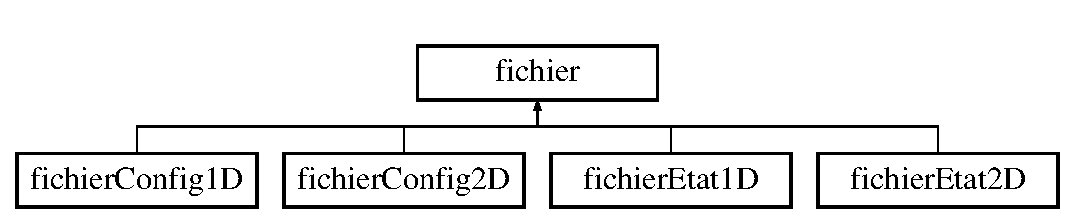
\includegraphics[height=2.000000cm]{classfichier}
\end{center}
\end{figure}
\subsection*{Fonctions membres publiques}
\begin{DoxyCompactItemize}
\item 
\mbox{\hyperlink{classfichier_a42004721e8f3931e39b12a513e12f48e}{fichier}} (const std\+::string nom)
\item 
virtual bool \mbox{\hyperlink{classfichier_ac54bfc9ea8c980c0b46bb291d3abdef4}{save}} (const \mbox{\hyperlink{class_cellular_automata}{Cellular\+Automata}} \&automate)=0
\item 
virtual bool \mbox{\hyperlink{classfichier_a6c246db929cf6532eb3f12c2b39574d5}{load}} (const \mbox{\hyperlink{class_cellular_automata}{Cellular\+Automata}} $\ast$automate)=0
\item 
virtual \mbox{\hyperlink{classfichier_aa9d389401e8d59b50377c472fb37b5da}{$\sim$fichier}} ()
\end{DoxyCompactItemize}
\subsection*{Attributs protégés}
\begin{DoxyCompactItemize}
\item 
std\+::string \mbox{\hyperlink{classfichier_a5507421c34a4358be0d0f842f74293fc}{nomF}}
\item 
std\+::fstream \mbox{\hyperlink{classfichier_ad4aa9acd482d376366be3d488e6af0ad}{f}}
\end{DoxyCompactItemize}


\subsection{Documentation des constructeurs et destructeur}
\mbox{\Hypertarget{classfichier_a42004721e8f3931e39b12a513e12f48e}\label{classfichier_a42004721e8f3931e39b12a513e12f48e}} 
\index{fichier@{fichier}!fichier@{fichier}}
\index{fichier@{fichier}!fichier@{fichier}}
\subsubsection{\texorpdfstring{fichier()}{fichier()}}
{\footnotesize\ttfamily fichier\+::fichier (\begin{DoxyParamCaption}\item[{const std\+::string}]{nom }\end{DoxyParamCaption})\hspace{0.3cm}{\ttfamily [inline]}}

\mbox{\Hypertarget{classfichier_aa9d389401e8d59b50377c472fb37b5da}\label{classfichier_aa9d389401e8d59b50377c472fb37b5da}} 
\index{fichier@{fichier}!````~fichier@{$\sim$fichier}}
\index{````~fichier@{$\sim$fichier}!fichier@{fichier}}
\subsubsection{\texorpdfstring{$\sim$fichier()}{~fichier()}}
{\footnotesize\ttfamily virtual fichier\+::$\sim$fichier (\begin{DoxyParamCaption}{ }\end{DoxyParamCaption})\hspace{0.3cm}{\ttfamily [inline]}, {\ttfamily [virtual]}}



\subsection{Documentation des fonctions membres}
\mbox{\Hypertarget{classfichier_a6c246db929cf6532eb3f12c2b39574d5}\label{classfichier_a6c246db929cf6532eb3f12c2b39574d5}} 
\index{fichier@{fichier}!load@{load}}
\index{load@{load}!fichier@{fichier}}
\subsubsection{\texorpdfstring{load()}{load()}}
{\footnotesize\ttfamily virtual bool fichier\+::load (\begin{DoxyParamCaption}\item[{const \mbox{\hyperlink{class_cellular_automata}{Cellular\+Automata}} $\ast$}]{automate }\end{DoxyParamCaption})\hspace{0.3cm}{\ttfamily [pure virtual]}}



Implémenté dans \mbox{\hyperlink{classfichier_config2_d_a90761ac1866815bd59b0f1730ce6bd5f}{fichier\+Config2D}}, \mbox{\hyperlink{classfichier_config1_d_a598c6ad0c9c16735b6c5843198dcc682}{fichier\+Config1D}}, \mbox{\hyperlink{classfichier_etat2_d_a1509a84b133ea169370a46301f74739e}{fichier\+Etat2D}}, et \mbox{\hyperlink{classfichier_etat1_d_a06c7ac08352e595eda7df415e50e66f8}{fichier\+Etat1D}}.

\mbox{\Hypertarget{classfichier_ac54bfc9ea8c980c0b46bb291d3abdef4}\label{classfichier_ac54bfc9ea8c980c0b46bb291d3abdef4}} 
\index{fichier@{fichier}!save@{save}}
\index{save@{save}!fichier@{fichier}}
\subsubsection{\texorpdfstring{save()}{save()}}
{\footnotesize\ttfamily virtual bool fichier\+::save (\begin{DoxyParamCaption}\item[{const \mbox{\hyperlink{class_cellular_automata}{Cellular\+Automata}} \&}]{automate }\end{DoxyParamCaption})\hspace{0.3cm}{\ttfamily [pure virtual]}}



Implémenté dans \mbox{\hyperlink{classfichier_config2_d_ac91d6cd20fd9edc6ed71684b8d5a1b40}{fichier\+Config2D}}, \mbox{\hyperlink{classfichier_config1_d_a759fa0735b22b3f5cceeb0fb414fc056}{fichier\+Config1D}}, \mbox{\hyperlink{classfichier_etat2_d_a0acba6c601772898383006d2c705a177}{fichier\+Etat2D}}, et \mbox{\hyperlink{classfichier_etat1_d_a120ee4b6234a18bdb88c5d60bd0ef5c0}{fichier\+Etat1D}}.



\subsection{Documentation des données membres}
\mbox{\Hypertarget{classfichier_ad4aa9acd482d376366be3d488e6af0ad}\label{classfichier_ad4aa9acd482d376366be3d488e6af0ad}} 
\index{fichier@{fichier}!f@{f}}
\index{f@{f}!fichier@{fichier}}
\subsubsection{\texorpdfstring{f}{f}}
{\footnotesize\ttfamily std\+::fstream fichier\+::f\hspace{0.3cm}{\ttfamily [protected]}}

\mbox{\Hypertarget{classfichier_a5507421c34a4358be0d0f842f74293fc}\label{classfichier_a5507421c34a4358be0d0f842f74293fc}} 
\index{fichier@{fichier}!nomF@{nomF}}
\index{nomF@{nomF}!fichier@{fichier}}
\subsubsection{\texorpdfstring{nomF}{nomF}}
{\footnotesize\ttfamily std\+::string fichier\+::nomF\hspace{0.3cm}{\ttfamily [protected]}}



La documentation de cette classe a été générée à partir du fichier suivant \+:\begin{DoxyCompactItemize}
\item 
C\+:/\+Users/maxn0/git/\+L\+O21/\+Auto\+Cell/\mbox{\hyperlink{fichier_8h}{fichier.\+h}}\end{DoxyCompactItemize}

\hypertarget{classfichier_config1_d}{}\section{Référence de la classe fichier\+Config1D}
\label{classfichier_config1_d}\index{fichier\+Config1D@{fichier\+Config1D}}


{\ttfamily \#include $<$fichier.\+h$>$}

Graphe d\textquotesingle{}héritage de fichier\+Config1D\+:\begin{figure}[H]
\begin{center}
\leavevmode
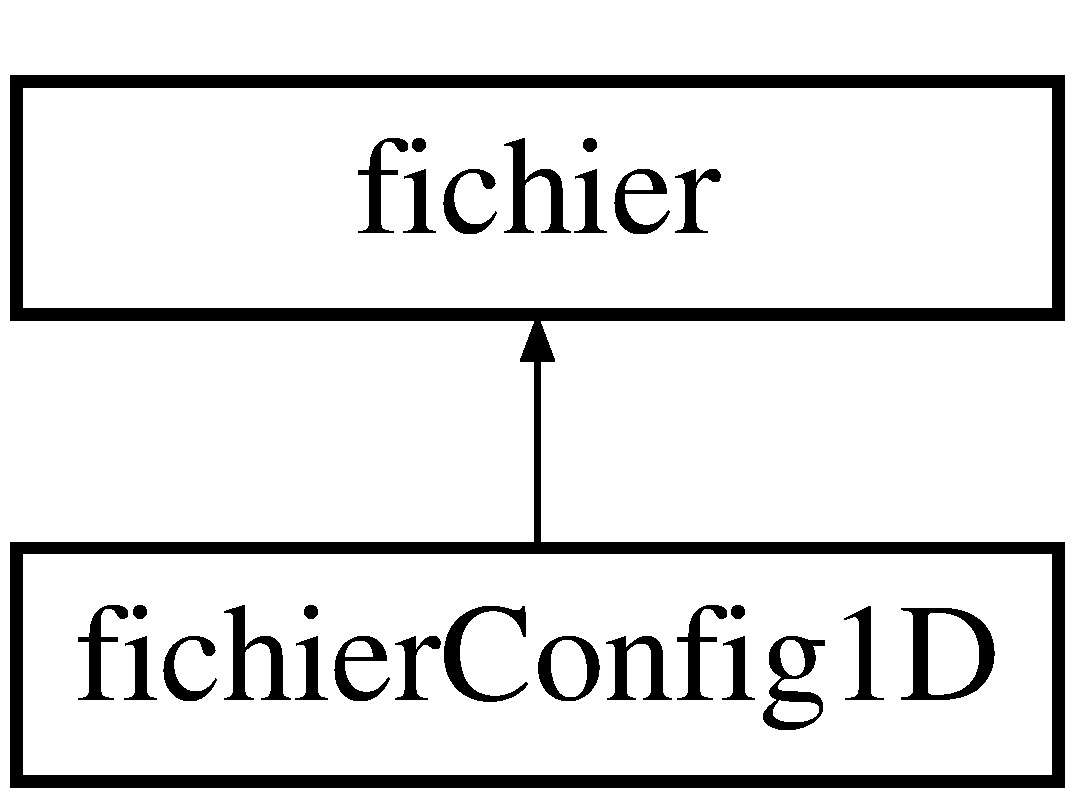
\includegraphics[height=2.000000cm]{classfichier_config1_d}
\end{center}
\end{figure}
\subsection*{Fonctions membres publiques}
\begin{DoxyCompactItemize}
\item 
\mbox{\hyperlink{classfichier_config1_d_ab762d4c2b8caeb4ae175ea04f696b94a}{fichier\+Config1D}} (const std\+::string nom)
\item 
bool \mbox{\hyperlink{classfichier_config1_d_a759fa0735b22b3f5cceeb0fb414fc056}{save}} (const \mbox{\hyperlink{class_cellular_automata}{Cellular\+Automata}} \&automate)
\item 
bool \mbox{\hyperlink{classfichier_config1_d_a598c6ad0c9c16735b6c5843198dcc682}{load}} (const \mbox{\hyperlink{class_cellular_automata}{Cellular\+Automata}} $\ast$automate)
\end{DoxyCompactItemize}
\subsection*{Membres hérités additionnels}


\subsection{Documentation des constructeurs et destructeur}
\mbox{\Hypertarget{classfichier_config1_d_ab762d4c2b8caeb4ae175ea04f696b94a}\label{classfichier_config1_d_ab762d4c2b8caeb4ae175ea04f696b94a}} 
\index{fichier\+Config1D@{fichier\+Config1D}!fichier\+Config1D@{fichier\+Config1D}}
\index{fichier\+Config1D@{fichier\+Config1D}!fichier\+Config1D@{fichier\+Config1D}}
\subsubsection{\texorpdfstring{fichier\+Config1\+D()}{fichierConfig1D()}}
{\footnotesize\ttfamily fichier\+Config1\+D\+::fichier\+Config1D (\begin{DoxyParamCaption}\item[{const std\+::string}]{nom }\end{DoxyParamCaption})\hspace{0.3cm}{\ttfamily [inline]}}



\subsection{Documentation des fonctions membres}
\mbox{\Hypertarget{classfichier_config1_d_a598c6ad0c9c16735b6c5843198dcc682}\label{classfichier_config1_d_a598c6ad0c9c16735b6c5843198dcc682}} 
\index{fichier\+Config1D@{fichier\+Config1D}!load@{load}}
\index{load@{load}!fichier\+Config1D@{fichier\+Config1D}}
\subsubsection{\texorpdfstring{load()}{load()}}
{\footnotesize\ttfamily bool fichier\+Config1\+D\+::load (\begin{DoxyParamCaption}\item[{const \mbox{\hyperlink{class_cellular_automata}{Cellular\+Automata}} $\ast$}]{automate }\end{DoxyParamCaption})\hspace{0.3cm}{\ttfamily [virtual]}}



Implémente \mbox{\hyperlink{classfichier_a6c246db929cf6532eb3f12c2b39574d5}{fichier}}.

\mbox{\Hypertarget{classfichier_config1_d_a759fa0735b22b3f5cceeb0fb414fc056}\label{classfichier_config1_d_a759fa0735b22b3f5cceeb0fb414fc056}} 
\index{fichier\+Config1D@{fichier\+Config1D}!save@{save}}
\index{save@{save}!fichier\+Config1D@{fichier\+Config1D}}
\subsubsection{\texorpdfstring{save()}{save()}}
{\footnotesize\ttfamily bool fichier\+Config1\+D\+::save (\begin{DoxyParamCaption}\item[{const \mbox{\hyperlink{class_cellular_automata}{Cellular\+Automata}} \&}]{automate }\end{DoxyParamCaption})\hspace{0.3cm}{\ttfamily [virtual]}}



Implémente \mbox{\hyperlink{classfichier_ac54bfc9ea8c980c0b46bb291d3abdef4}{fichier}}.



La documentation de cette classe a été générée à partir des fichiers suivants \+:\begin{DoxyCompactItemize}
\item 
C\+:/\+Users/maxn0/git/\+L\+O21/\+Auto\+Cell/\mbox{\hyperlink{fichier_8h}{fichier.\+h}}\item 
C\+:/\+Users/maxn0/git/\+L\+O21/\+Auto\+Cell/\mbox{\hyperlink{fichier_8cpp}{fichier.\+cpp}}\end{DoxyCompactItemize}

\hypertarget{classfichier_config2_d}{}\section{Référence de la classe fichier\+Config2D}
\label{classfichier_config2_d}\index{fichier\+Config2D@{fichier\+Config2D}}


{\ttfamily \#include $<$fichier.\+h$>$}

Graphe d\textquotesingle{}héritage de fichier\+Config2D\+:\begin{figure}[H]
\begin{center}
\leavevmode
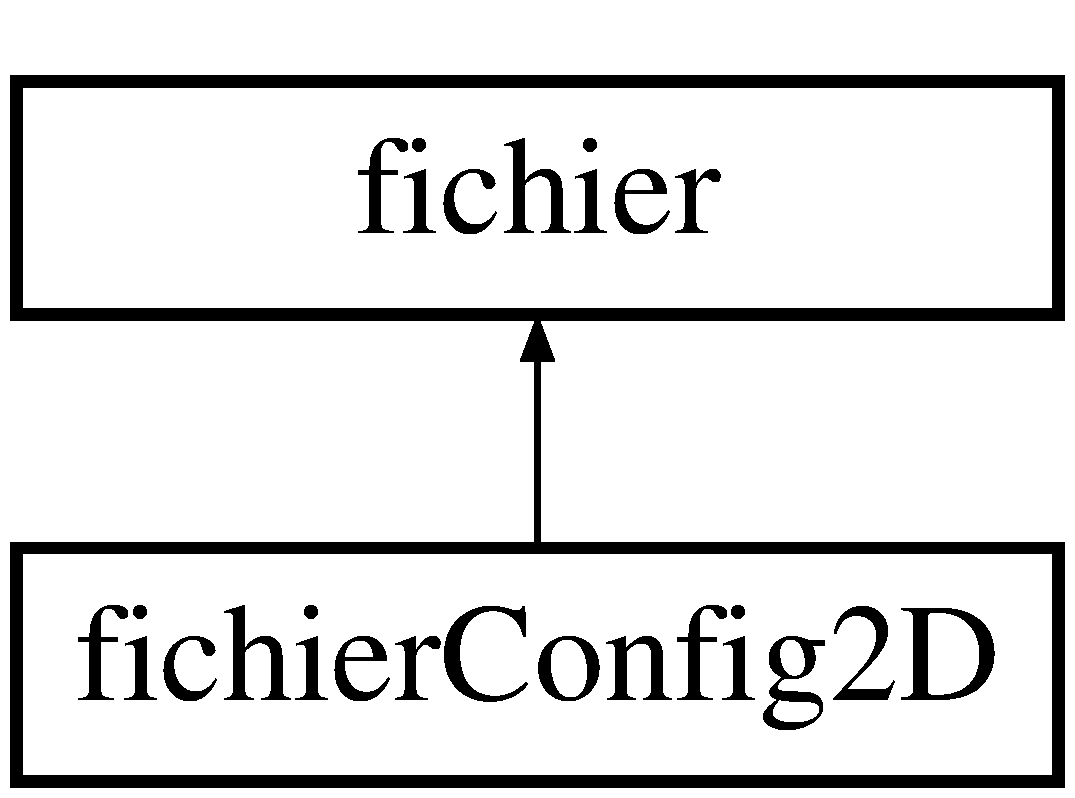
\includegraphics[height=2.000000cm]{classfichier_config2_d}
\end{center}
\end{figure}
\subsection*{Fonctions membres publiques}
\begin{DoxyCompactItemize}
\item 
\mbox{\hyperlink{classfichier_config2_d_a4614bc2c0ab608204eaddc468337d80d}{fichier\+Config2D}} (const std\+::string nom)
\item 
bool \mbox{\hyperlink{classfichier_config2_d_ac91d6cd20fd9edc6ed71684b8d5a1b40}{save}} (const \mbox{\hyperlink{class_cellular_automata}{Cellular\+Automata}} \&automate)
\item 
bool \mbox{\hyperlink{classfichier_config2_d_a90761ac1866815bd59b0f1730ce6bd5f}{load}} (const \mbox{\hyperlink{class_cellular_automata}{Cellular\+Automata}} $\ast$automate)
\end{DoxyCompactItemize}
\subsection*{Membres hérités additionnels}


\subsection{Documentation des constructeurs et destructeur}
\mbox{\Hypertarget{classfichier_config2_d_a4614bc2c0ab608204eaddc468337d80d}\label{classfichier_config2_d_a4614bc2c0ab608204eaddc468337d80d}} 
\index{fichier\+Config2D@{fichier\+Config2D}!fichier\+Config2D@{fichier\+Config2D}}
\index{fichier\+Config2D@{fichier\+Config2D}!fichier\+Config2D@{fichier\+Config2D}}
\subsubsection{\texorpdfstring{fichier\+Config2\+D()}{fichierConfig2D()}}
{\footnotesize\ttfamily fichier\+Config2\+D\+::fichier\+Config2D (\begin{DoxyParamCaption}\item[{const std\+::string}]{nom }\end{DoxyParamCaption})\hspace{0.3cm}{\ttfamily [inline]}}



\subsection{Documentation des fonctions membres}
\mbox{\Hypertarget{classfichier_config2_d_a90761ac1866815bd59b0f1730ce6bd5f}\label{classfichier_config2_d_a90761ac1866815bd59b0f1730ce6bd5f}} 
\index{fichier\+Config2D@{fichier\+Config2D}!load@{load}}
\index{load@{load}!fichier\+Config2D@{fichier\+Config2D}}
\subsubsection{\texorpdfstring{load()}{load()}}
{\footnotesize\ttfamily bool fichier\+Config2\+D\+::load (\begin{DoxyParamCaption}\item[{const \mbox{\hyperlink{class_cellular_automata}{Cellular\+Automata}} $\ast$}]{automate }\end{DoxyParamCaption})\hspace{0.3cm}{\ttfamily [virtual]}}



Implémente \mbox{\hyperlink{classfichier_a6c246db929cf6532eb3f12c2b39574d5}{fichier}}.

\mbox{\Hypertarget{classfichier_config2_d_ac91d6cd20fd9edc6ed71684b8d5a1b40}\label{classfichier_config2_d_ac91d6cd20fd9edc6ed71684b8d5a1b40}} 
\index{fichier\+Config2D@{fichier\+Config2D}!save@{save}}
\index{save@{save}!fichier\+Config2D@{fichier\+Config2D}}
\subsubsection{\texorpdfstring{save()}{save()}}
{\footnotesize\ttfamily bool fichier\+Config2\+D\+::save (\begin{DoxyParamCaption}\item[{const \mbox{\hyperlink{class_cellular_automata}{Cellular\+Automata}} \&}]{automate }\end{DoxyParamCaption})\hspace{0.3cm}{\ttfamily [virtual]}}



Implémente \mbox{\hyperlink{classfichier_ac54bfc9ea8c980c0b46bb291d3abdef4}{fichier}}.



La documentation de cette classe a été générée à partir des fichiers suivants \+:\begin{DoxyCompactItemize}
\item 
C\+:/\+Users/maxn0/git/\+L\+O21/\+Auto\+Cell/\mbox{\hyperlink{fichier_8h}{fichier.\+h}}\item 
C\+:/\+Users/maxn0/git/\+L\+O21/\+Auto\+Cell/\mbox{\hyperlink{fichier_8cpp}{fichier.\+cpp}}\end{DoxyCompactItemize}

\hypertarget{classfichier_etat1_d}{}\section{Référence de la classe fichier\+Etat1D}
\label{classfichier_etat1_d}\index{fichier\+Etat1D@{fichier\+Etat1D}}


{\ttfamily \#include $<$fichier.\+h$>$}

Graphe d\textquotesingle{}héritage de fichier\+Etat1D\+:\begin{figure}[H]
\begin{center}
\leavevmode
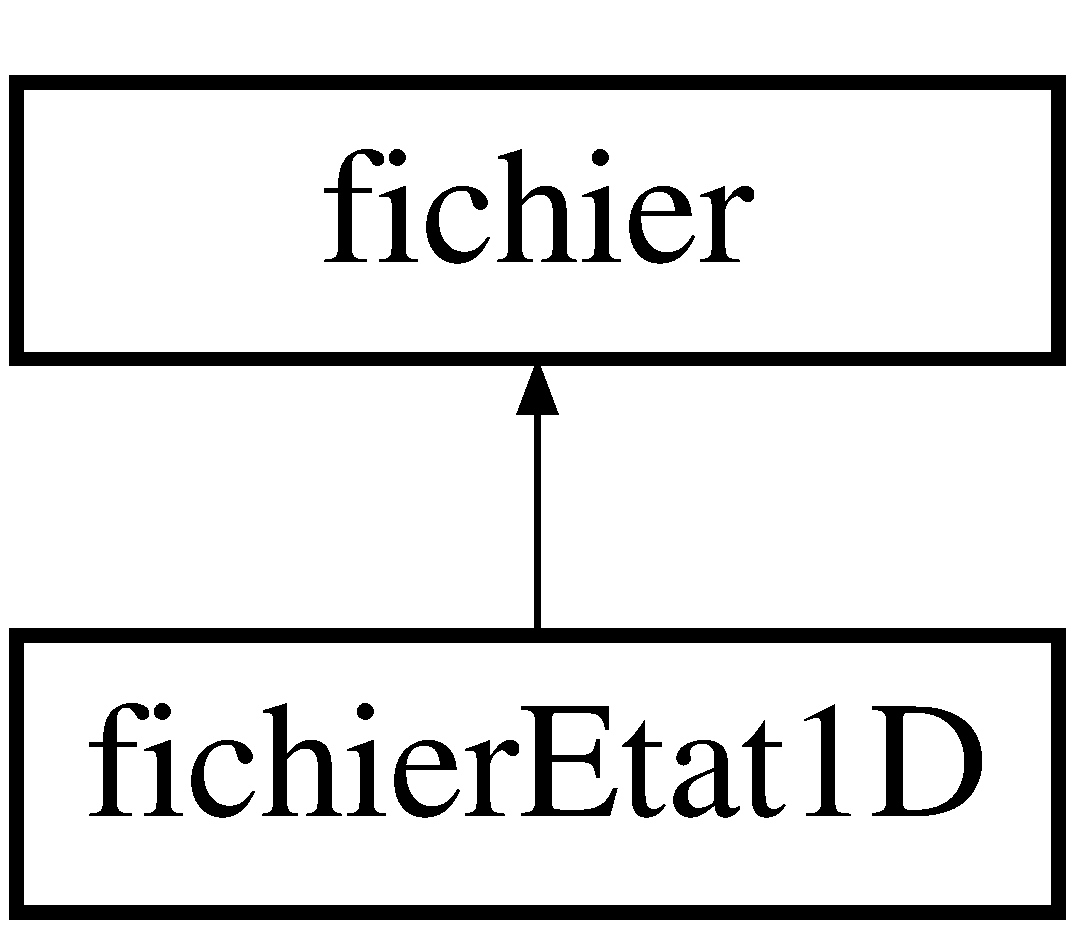
\includegraphics[height=2.000000cm]{classfichier_etat1_d}
\end{center}
\end{figure}
\subsection*{Fonctions membres publiques}
\begin{DoxyCompactItemize}
\item 
\mbox{\hyperlink{classfichier_etat1_d_ac51077398acac276b0b8dd10dea2228e}{fichier\+Etat1D}} (const std\+::string nom)
\item 
bool \mbox{\hyperlink{classfichier_etat1_d_a120ee4b6234a18bdb88c5d60bd0ef5c0}{save}} (const \mbox{\hyperlink{class_cellular_automata}{Cellular\+Automata}} \&automate)
\item 
bool \mbox{\hyperlink{classfichier_etat1_d_a06c7ac08352e595eda7df415e50e66f8}{load}} (const \mbox{\hyperlink{class_cellular_automata}{Cellular\+Automata}} $\ast$automate)
\end{DoxyCompactItemize}
\subsection*{Membres hérités additionnels}


\subsection{Documentation des constructeurs et destructeur}
\mbox{\Hypertarget{classfichier_etat1_d_ac51077398acac276b0b8dd10dea2228e}\label{classfichier_etat1_d_ac51077398acac276b0b8dd10dea2228e}} 
\index{fichier\+Etat1D@{fichier\+Etat1D}!fichier\+Etat1D@{fichier\+Etat1D}}
\index{fichier\+Etat1D@{fichier\+Etat1D}!fichier\+Etat1D@{fichier\+Etat1D}}
\subsubsection{\texorpdfstring{fichier\+Etat1\+D()}{fichierEtat1D()}}
{\footnotesize\ttfamily fichier\+Etat1\+D\+::fichier\+Etat1D (\begin{DoxyParamCaption}\item[{const std\+::string}]{nom }\end{DoxyParamCaption})\hspace{0.3cm}{\ttfamily [inline]}}



\subsection{Documentation des fonctions membres}
\mbox{\Hypertarget{classfichier_etat1_d_a06c7ac08352e595eda7df415e50e66f8}\label{classfichier_etat1_d_a06c7ac08352e595eda7df415e50e66f8}} 
\index{fichier\+Etat1D@{fichier\+Etat1D}!load@{load}}
\index{load@{load}!fichier\+Etat1D@{fichier\+Etat1D}}
\subsubsection{\texorpdfstring{load()}{load()}}
{\footnotesize\ttfamily bool fichier\+Etat1\+D\+::load (\begin{DoxyParamCaption}\item[{const \mbox{\hyperlink{class_cellular_automata}{Cellular\+Automata}} $\ast$}]{automate }\end{DoxyParamCaption})\hspace{0.3cm}{\ttfamily [virtual]}}



Implémente \mbox{\hyperlink{classfichier_a6c246db929cf6532eb3f12c2b39574d5}{fichier}}.

\mbox{\Hypertarget{classfichier_etat1_d_a120ee4b6234a18bdb88c5d60bd0ef5c0}\label{classfichier_etat1_d_a120ee4b6234a18bdb88c5d60bd0ef5c0}} 
\index{fichier\+Etat1D@{fichier\+Etat1D}!save@{save}}
\index{save@{save}!fichier\+Etat1D@{fichier\+Etat1D}}
\subsubsection{\texorpdfstring{save()}{save()}}
{\footnotesize\ttfamily bool fichier\+Etat1\+D\+::save (\begin{DoxyParamCaption}\item[{const \mbox{\hyperlink{class_cellular_automata}{Cellular\+Automata}} \&}]{automate }\end{DoxyParamCaption})\hspace{0.3cm}{\ttfamily [virtual]}}



Implémente \mbox{\hyperlink{classfichier_ac54bfc9ea8c980c0b46bb291d3abdef4}{fichier}}.



La documentation de cette classe a été générée à partir des fichiers suivants \+:\begin{DoxyCompactItemize}
\item 
C\+:/\+Users/maxn0/git/\+L\+O21/\+Auto\+Cell/\mbox{\hyperlink{fichier_8h}{fichier.\+h}}\item 
C\+:/\+Users/maxn0/git/\+L\+O21/\+Auto\+Cell/\mbox{\hyperlink{fichier_8cpp}{fichier.\+cpp}}\end{DoxyCompactItemize}

\hypertarget{classfichier_etat2_d}{}\section{Référence de la classe fichier\+Etat2D}
\label{classfichier_etat2_d}\index{fichier\+Etat2D@{fichier\+Etat2D}}


{\ttfamily \#include $<$fichier.\+h$>$}

Graphe d\textquotesingle{}héritage de fichier\+Etat2D\+:\begin{figure}[H]
\begin{center}
\leavevmode
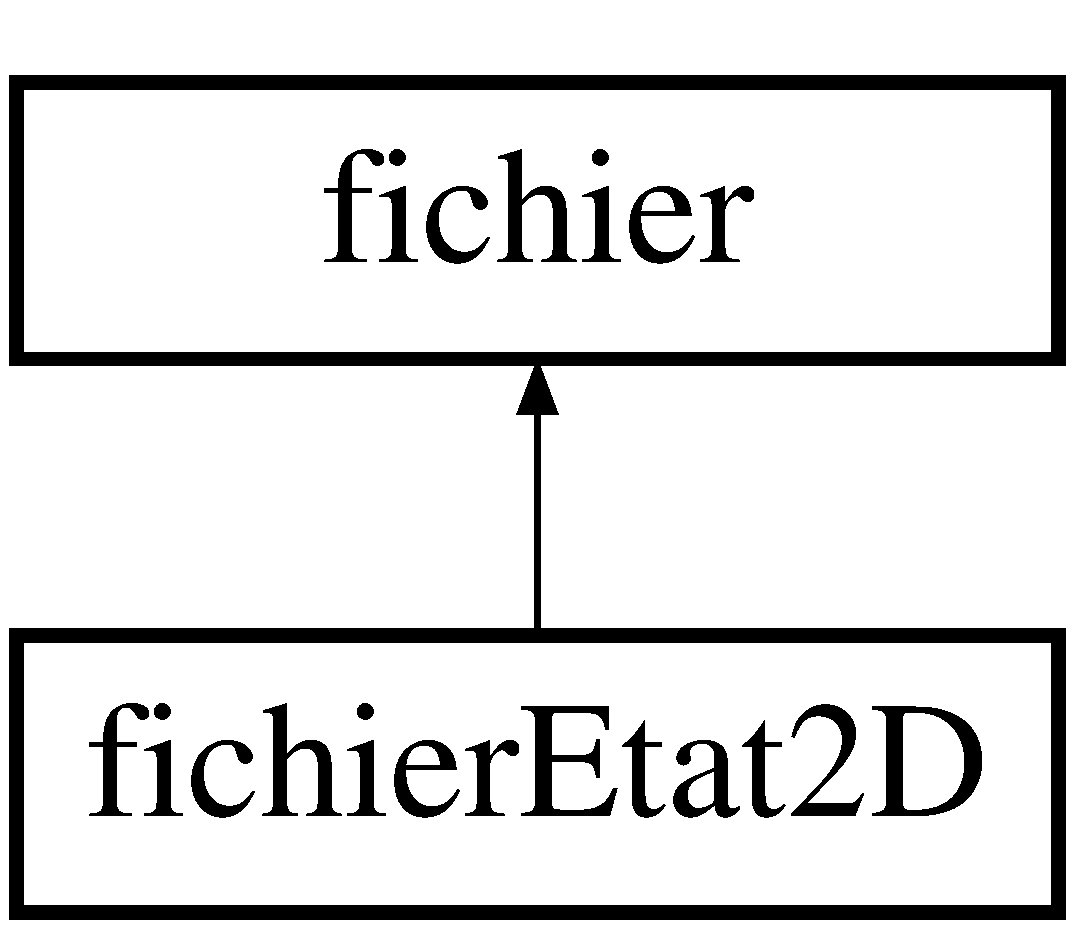
\includegraphics[height=2.000000cm]{classfichier_etat2_d}
\end{center}
\end{figure}
\subsection*{Fonctions membres publiques}
\begin{DoxyCompactItemize}
\item 
\mbox{\hyperlink{classfichier_etat2_d_a0d47202c1e69bcf5a5380037b3688b2c}{fichier\+Etat2D}} (const std\+::string nom)
\item 
bool \mbox{\hyperlink{classfichier_etat2_d_a0acba6c601772898383006d2c705a177}{save}} (const \mbox{\hyperlink{class_cellular_automata}{Cellular\+Automata}} \&automate)
\item 
bool \mbox{\hyperlink{classfichier_etat2_d_a1509a84b133ea169370a46301f74739e}{load}} (const \mbox{\hyperlink{class_cellular_automata}{Cellular\+Automata}} $\ast$automate)
\end{DoxyCompactItemize}
\subsection*{Membres hérités additionnels}


\subsection{Documentation des constructeurs et destructeur}
\mbox{\Hypertarget{classfichier_etat2_d_a0d47202c1e69bcf5a5380037b3688b2c}\label{classfichier_etat2_d_a0d47202c1e69bcf5a5380037b3688b2c}} 
\index{fichier\+Etat2D@{fichier\+Etat2D}!fichier\+Etat2D@{fichier\+Etat2D}}
\index{fichier\+Etat2D@{fichier\+Etat2D}!fichier\+Etat2D@{fichier\+Etat2D}}
\subsubsection{\texorpdfstring{fichier\+Etat2\+D()}{fichierEtat2D()}}
{\footnotesize\ttfamily fichier\+Etat2\+D\+::fichier\+Etat2D (\begin{DoxyParamCaption}\item[{const std\+::string}]{nom }\end{DoxyParamCaption})\hspace{0.3cm}{\ttfamily [inline]}}



\subsection{Documentation des fonctions membres}
\mbox{\Hypertarget{classfichier_etat2_d_a1509a84b133ea169370a46301f74739e}\label{classfichier_etat2_d_a1509a84b133ea169370a46301f74739e}} 
\index{fichier\+Etat2D@{fichier\+Etat2D}!load@{load}}
\index{load@{load}!fichier\+Etat2D@{fichier\+Etat2D}}
\subsubsection{\texorpdfstring{load()}{load()}}
{\footnotesize\ttfamily bool fichier\+Etat2\+D\+::load (\begin{DoxyParamCaption}\item[{const \mbox{\hyperlink{class_cellular_automata}{Cellular\+Automata}} $\ast$}]{automate }\end{DoxyParamCaption})\hspace{0.3cm}{\ttfamily [virtual]}}



Implémente \mbox{\hyperlink{classfichier_a6c246db929cf6532eb3f12c2b39574d5}{fichier}}.

\mbox{\Hypertarget{classfichier_etat2_d_a0acba6c601772898383006d2c705a177}\label{classfichier_etat2_d_a0acba6c601772898383006d2c705a177}} 
\index{fichier\+Etat2D@{fichier\+Etat2D}!save@{save}}
\index{save@{save}!fichier\+Etat2D@{fichier\+Etat2D}}
\subsubsection{\texorpdfstring{save()}{save()}}
{\footnotesize\ttfamily bool fichier\+Etat2\+D\+::save (\begin{DoxyParamCaption}\item[{const \mbox{\hyperlink{class_cellular_automata}{Cellular\+Automata}} \&}]{automate }\end{DoxyParamCaption})\hspace{0.3cm}{\ttfamily [virtual]}}



Implémente \mbox{\hyperlink{classfichier_ac54bfc9ea8c980c0b46bb291d3abdef4}{fichier}}.



La documentation de cette classe a été générée à partir des fichiers suivants \+:\begin{DoxyCompactItemize}
\item 
C\+:/\+Users/maxn0/git/\+L\+O21/\+Auto\+Cell/\mbox{\hyperlink{fichier_8h}{fichier.\+h}}\item 
C\+:/\+Users/maxn0/git/\+L\+O21/\+Auto\+Cell/\mbox{\hyperlink{fichier_8cpp}{fichier.\+cpp}}\end{DoxyCompactItemize}

\hypertarget{class_game_of_life}{}\section{Référence de la classe Game\+Of\+Life}
\label{class_game_of_life}\index{Game\+Of\+Life@{Game\+Of\+Life}}


{\ttfamily \#include $<$transitionrule.\+h$>$}

Graphe d\textquotesingle{}héritage de Game\+Of\+Life\+:\begin{figure}[H]
\begin{center}
\leavevmode
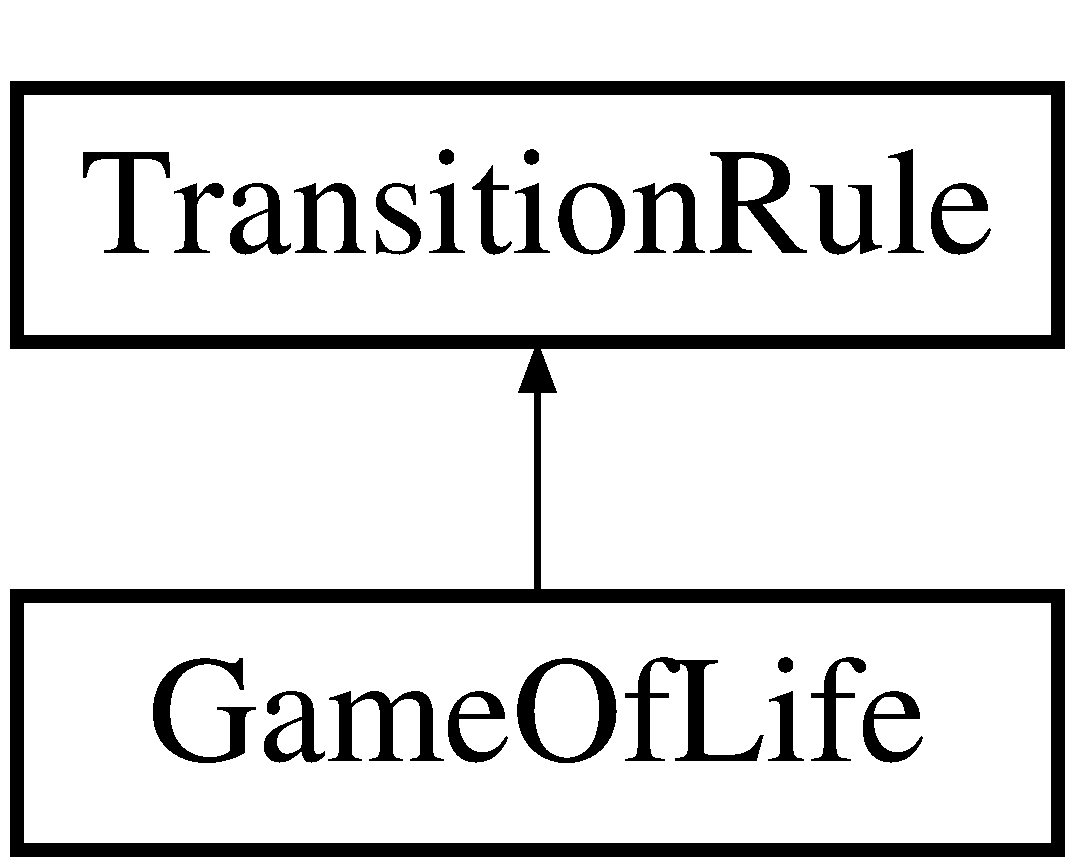
\includegraphics[height=2.000000cm]{class_game_of_life}
\end{center}
\end{figure}
\subsection*{Fonctions membres publiques}
\begin{DoxyCompactItemize}
\item 
void \mbox{\hyperlink{class_game_of_life_a12e6db1719e64adc023e1a7d2976d38d}{Transition\+Cellule}} (\mbox{\hyperlink{class_cell}{Cell}} const \&depart, \mbox{\hyperlink{class_cell}{Cell}} \&arrivee) const override
\item 
\mbox{\hyperlink{class_game_of_life_a033f778ad4b391bbf04dfa937f7b11df}{Game\+Of\+Life}} (unsigned int min\+Voisins\+Vivants, unsigned int max\+Voisins\+Vivants)
\item 
std\+::string \mbox{\hyperlink{class_game_of_life_a636421a27cb52e9f7ec161d141809919}{get\+Transition}} () const override
\item 
unsigned int \mbox{\hyperlink{class_game_of_life_afb8e0ee780b7e187266060cf9bec0578}{get\+Nb\+Etats}} () const
\item 
\mbox{\hyperlink{class_game_of_life_a3006eb8600b82f3deff3b8efe6725569}{$\sim$\+Game\+Of\+Life}} ()=default
\end{DoxyCompactItemize}
\subsection*{Attributs protégés}
\begin{DoxyCompactItemize}
\item 
unsigned int \mbox{\hyperlink{class_game_of_life_a851bf99201f554c12cdedf9fa227c321}{m\+\_\+min\+Voisins\+Vivants}}
\item 
unsigned int \mbox{\hyperlink{class_game_of_life_ad10ffab0e8d12ccac18ec5d4bd587fcc}{m\+\_\+max\+Voisins\+Vivants}}
\end{DoxyCompactItemize}


\subsection{Documentation des constructeurs et destructeur}
\mbox{\Hypertarget{class_game_of_life_a033f778ad4b391bbf04dfa937f7b11df}\label{class_game_of_life_a033f778ad4b391bbf04dfa937f7b11df}} 
\index{Game\+Of\+Life@{Game\+Of\+Life}!Game\+Of\+Life@{Game\+Of\+Life}}
\index{Game\+Of\+Life@{Game\+Of\+Life}!Game\+Of\+Life@{Game\+Of\+Life}}
\subsubsection{\texorpdfstring{Game\+Of\+Life()}{GameOfLife()}}
{\footnotesize\ttfamily Game\+Of\+Life\+::\+Game\+Of\+Life (\begin{DoxyParamCaption}\item[{unsigned int}]{min\+Voisins\+Vivants,  }\item[{unsigned int}]{max\+Voisins\+Vivants }\end{DoxyParamCaption})\hspace{0.3cm}{\ttfamily [inline]}}

\mbox{\Hypertarget{class_game_of_life_a3006eb8600b82f3deff3b8efe6725569}\label{class_game_of_life_a3006eb8600b82f3deff3b8efe6725569}} 
\index{Game\+Of\+Life@{Game\+Of\+Life}!````~Game\+Of\+Life@{$\sim$\+Game\+Of\+Life}}
\index{````~Game\+Of\+Life@{$\sim$\+Game\+Of\+Life}!Game\+Of\+Life@{Game\+Of\+Life}}
\subsubsection{\texorpdfstring{$\sim$\+Game\+Of\+Life()}{~GameOfLife()}}
{\footnotesize\ttfamily Game\+Of\+Life\+::$\sim$\+Game\+Of\+Life (\begin{DoxyParamCaption}{ }\end{DoxyParamCaption})\hspace{0.3cm}{\ttfamily [default]}}



\subsection{Documentation des fonctions membres}
\mbox{\Hypertarget{class_game_of_life_afb8e0ee780b7e187266060cf9bec0578}\label{class_game_of_life_afb8e0ee780b7e187266060cf9bec0578}} 
\index{Game\+Of\+Life@{Game\+Of\+Life}!get\+Nb\+Etats@{get\+Nb\+Etats}}
\index{get\+Nb\+Etats@{get\+Nb\+Etats}!Game\+Of\+Life@{Game\+Of\+Life}}
\subsubsection{\texorpdfstring{get\+Nb\+Etats()}{getNbEtats()}}
{\footnotesize\ttfamily unsigned int Game\+Of\+Life\+::get\+Nb\+Etats (\begin{DoxyParamCaption}{ }\end{DoxyParamCaption}) const\hspace{0.3cm}{\ttfamily [inline]}, {\ttfamily [virtual]}}



Implémente \mbox{\hyperlink{class_transition_rule_ad5bbcc6ef292bb079d8980f00d011a90}{Transition\+Rule}}.

\mbox{\Hypertarget{class_game_of_life_a636421a27cb52e9f7ec161d141809919}\label{class_game_of_life_a636421a27cb52e9f7ec161d141809919}} 
\index{Game\+Of\+Life@{Game\+Of\+Life}!get\+Transition@{get\+Transition}}
\index{get\+Transition@{get\+Transition}!Game\+Of\+Life@{Game\+Of\+Life}}
\subsubsection{\texorpdfstring{get\+Transition()}{getTransition()}}
{\footnotesize\ttfamily std\+::string Game\+Of\+Life\+::get\+Transition (\begin{DoxyParamCaption}{ }\end{DoxyParamCaption}) const\hspace{0.3cm}{\ttfamily [override]}, {\ttfamily [virtual]}}



Implémente \mbox{\hyperlink{class_transition_rule_af537bee6cca486c754ee94855242328c}{Transition\+Rule}}.

\mbox{\Hypertarget{class_game_of_life_a12e6db1719e64adc023e1a7d2976d38d}\label{class_game_of_life_a12e6db1719e64adc023e1a7d2976d38d}} 
\index{Game\+Of\+Life@{Game\+Of\+Life}!Transition\+Cellule@{Transition\+Cellule}}
\index{Transition\+Cellule@{Transition\+Cellule}!Game\+Of\+Life@{Game\+Of\+Life}}
\subsubsection{\texorpdfstring{Transition\+Cellule()}{TransitionCellule()}}
{\footnotesize\ttfamily void Game\+Of\+Life\+::\+Transition\+Cellule (\begin{DoxyParamCaption}\item[{\mbox{\hyperlink{class_cell}{Cell}} const \&}]{depart,  }\item[{\mbox{\hyperlink{class_cell}{Cell}} \&}]{arrivee }\end{DoxyParamCaption}) const\hspace{0.3cm}{\ttfamily [override]}, {\ttfamily [virtual]}}



Implémente \mbox{\hyperlink{class_transition_rule_a2b82a75ef494adc91b28755d55666e7a}{Transition\+Rule}}.



\subsection{Documentation des données membres}
\mbox{\Hypertarget{class_game_of_life_ad10ffab0e8d12ccac18ec5d4bd587fcc}\label{class_game_of_life_ad10ffab0e8d12ccac18ec5d4bd587fcc}} 
\index{Game\+Of\+Life@{Game\+Of\+Life}!m\+\_\+max\+Voisins\+Vivants@{m\+\_\+max\+Voisins\+Vivants}}
\index{m\+\_\+max\+Voisins\+Vivants@{m\+\_\+max\+Voisins\+Vivants}!Game\+Of\+Life@{Game\+Of\+Life}}
\subsubsection{\texorpdfstring{m\+\_\+max\+Voisins\+Vivants}{m\_maxVoisinsVivants}}
{\footnotesize\ttfamily unsigned int Game\+Of\+Life\+::m\+\_\+max\+Voisins\+Vivants\hspace{0.3cm}{\ttfamily [protected]}}

\mbox{\Hypertarget{class_game_of_life_a851bf99201f554c12cdedf9fa227c321}\label{class_game_of_life_a851bf99201f554c12cdedf9fa227c321}} 
\index{Game\+Of\+Life@{Game\+Of\+Life}!m\+\_\+min\+Voisins\+Vivants@{m\+\_\+min\+Voisins\+Vivants}}
\index{m\+\_\+min\+Voisins\+Vivants@{m\+\_\+min\+Voisins\+Vivants}!Game\+Of\+Life@{Game\+Of\+Life}}
\subsubsection{\texorpdfstring{m\+\_\+min\+Voisins\+Vivants}{m\_minVoisinsVivants}}
{\footnotesize\ttfamily unsigned int Game\+Of\+Life\+::m\+\_\+min\+Voisins\+Vivants\hspace{0.3cm}{\ttfamily [protected]}}



La documentation de cette classe a été générée à partir des fichiers suivants \+:\begin{DoxyCompactItemize}
\item 
C\+:/\+Users/maxn0/git/\+L\+O21/\+Auto\+Cell/\mbox{\hyperlink{transitionrule_8h}{transitionrule.\+h}}\item 
C\+:/\+Users/maxn0/git/\+L\+O21/\+Auto\+Cell/\mbox{\hyperlink{transitionrule_8cpp}{transitionrule.\+cpp}}\end{DoxyCompactItemize}

\hypertarget{class_generateur_etat}{}\section{Référence de la classe Generateur\+Etat}
\label{class_generateur_etat}\index{Generateur\+Etat@{Generateur\+Etat}}


{\ttfamily \#include $<$generateuretat.\+h$>$}

Graphe d\textquotesingle{}héritage de Generateur\+Etat\+:\begin{figure}[H]
\begin{center}
\leavevmode
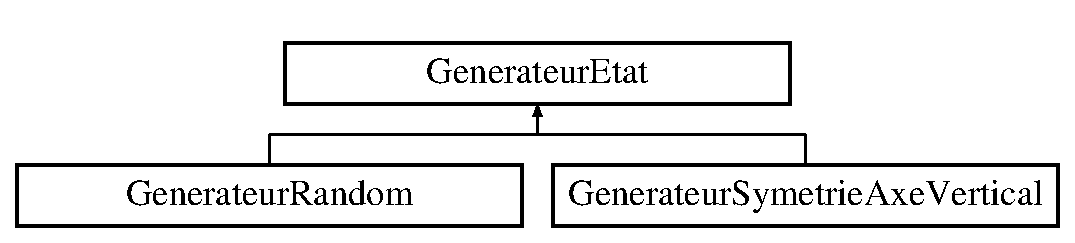
\includegraphics[height=2.000000cm]{class_generateur_etat}
\end{center}
\end{figure}
\subsection*{Fonctions membres publiques}
\begin{DoxyCompactItemize}
\item 
\mbox{\hyperlink{class_generateur_etat_a6ecebc169446d7f5fa40ed37af5abdaf}{Generateur\+Etat}} ()=default
\item 
virtual void \mbox{\hyperlink{class_generateur_etat_a0698d6706e0aaa2e597bdaf280806835}{Generer\+Etat}} (int nb\+Etats, \mbox{\hyperlink{class_etat}{Etat}} \&grille) const =0
\item 
virtual \mbox{\hyperlink{class_generateur_etat_a1ba21b5a12fa8855136363e338209d34}{$\sim$\+Generateur\+Etat}} ()=default
\end{DoxyCompactItemize}


\subsection{Documentation des constructeurs et destructeur}
\mbox{\Hypertarget{class_generateur_etat_a6ecebc169446d7f5fa40ed37af5abdaf}\label{class_generateur_etat_a6ecebc169446d7f5fa40ed37af5abdaf}} 
\index{Generateur\+Etat@{Generateur\+Etat}!Generateur\+Etat@{Generateur\+Etat}}
\index{Generateur\+Etat@{Generateur\+Etat}!Generateur\+Etat@{Generateur\+Etat}}
\subsubsection{\texorpdfstring{Generateur\+Etat()}{GenerateurEtat()}}
{\footnotesize\ttfamily Generateur\+Etat\+::\+Generateur\+Etat (\begin{DoxyParamCaption}{ }\end{DoxyParamCaption})\hspace{0.3cm}{\ttfamily [default]}}

\mbox{\Hypertarget{class_generateur_etat_a1ba21b5a12fa8855136363e338209d34}\label{class_generateur_etat_a1ba21b5a12fa8855136363e338209d34}} 
\index{Generateur\+Etat@{Generateur\+Etat}!````~Generateur\+Etat@{$\sim$\+Generateur\+Etat}}
\index{````~Generateur\+Etat@{$\sim$\+Generateur\+Etat}!Generateur\+Etat@{Generateur\+Etat}}
\subsubsection{\texorpdfstring{$\sim$\+Generateur\+Etat()}{~GenerateurEtat()}}
{\footnotesize\ttfamily virtual Generateur\+Etat\+::$\sim$\+Generateur\+Etat (\begin{DoxyParamCaption}{ }\end{DoxyParamCaption})\hspace{0.3cm}{\ttfamily [virtual]}, {\ttfamily [default]}}



\subsection{Documentation des fonctions membres}
\mbox{\Hypertarget{class_generateur_etat_a0698d6706e0aaa2e597bdaf280806835}\label{class_generateur_etat_a0698d6706e0aaa2e597bdaf280806835}} 
\index{Generateur\+Etat@{Generateur\+Etat}!Generer\+Etat@{Generer\+Etat}}
\index{Generer\+Etat@{Generer\+Etat}!Generateur\+Etat@{Generateur\+Etat}}
\subsubsection{\texorpdfstring{Generer\+Etat()}{GenererEtat()}}
{\footnotesize\ttfamily virtual void Generateur\+Etat\+::\+Generer\+Etat (\begin{DoxyParamCaption}\item[{int}]{nb\+Etats,  }\item[{\mbox{\hyperlink{class_etat}{Etat}} \&}]{grille }\end{DoxyParamCaption}) const\hspace{0.3cm}{\ttfamily [pure virtual]}}



Implémenté dans \mbox{\hyperlink{class_generateur_symetrie_axe_vertical_ae782046a73fc7624212c3c5988de949f}{Generateur\+Symetrie\+Axe\+Vertical}}, et \mbox{\hyperlink{class_generateur_random_ab110072502487c78f0b7dc0c7f2241c7}{Generateur\+Random}}.



La documentation de cette classe a été générée à partir du fichier suivant \+:\begin{DoxyCompactItemize}
\item 
C\+:/\+Users/maxn0/git/\+L\+O21/\+Auto\+Cell/\mbox{\hyperlink{generateuretat_8h}{generateuretat.\+h}}\end{DoxyCompactItemize}

\hypertarget{class_generateur_random}{}\section{Generateur\+Random Class Reference}
\label{class_generateur_random}\index{Generateur\+Random@{Generateur\+Random}}
Inheritance diagram for Generateur\+Random\+:\begin{figure}[H]
\begin{center}
\leavevmode
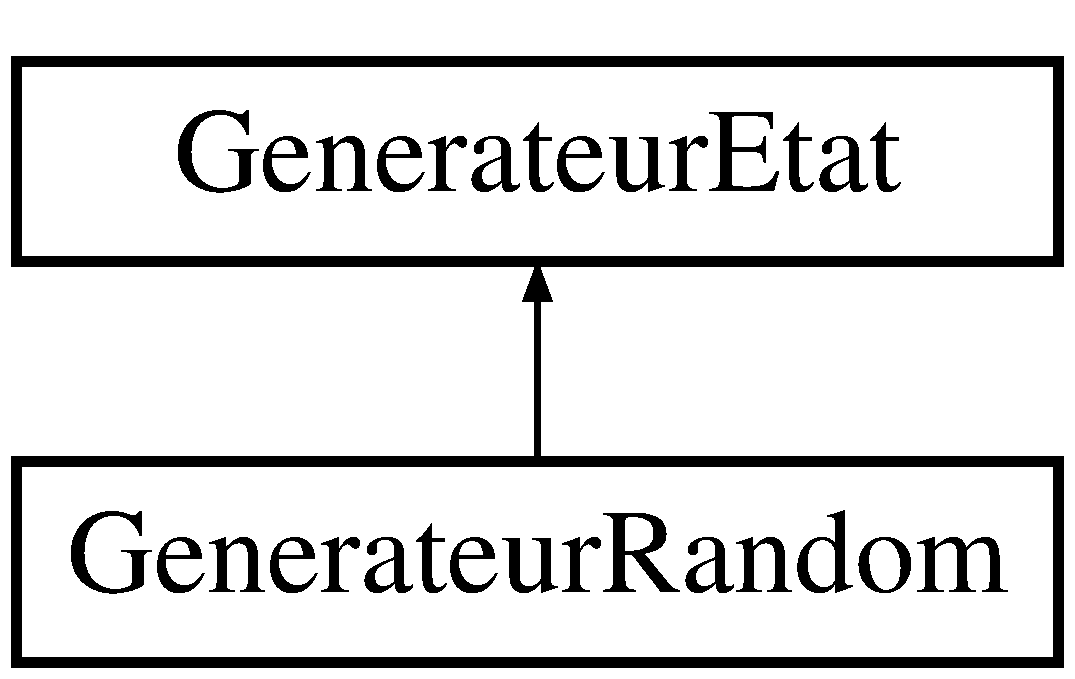
\includegraphics[height=2.000000cm]{class_generateur_random}
\end{center}
\end{figure}
\subsection*{Public Member Functions}
\begin{DoxyCompactItemize}
\item 
\mbox{\Hypertarget{class_generateur_random_ad6c15ee02504f5aa230068e5b1fa7a6b}\label{class_generateur_random_ad6c15ee02504f5aa230068e5b1fa7a6b}} 
void {\bfseries Generer\+Etat} (int nb\+Etat, std\+::vector$<$ std\+::vector$<$ \mbox{\hyperlink{class_cell}{Cell}} $>$$>$ \&tab) override
\end{DoxyCompactItemize}


The documentation for this class was generated from the following files\+:\begin{DoxyCompactItemize}
\item 
C\+:/\+Users/maxn0/git/\+L\+O21/\+Auto\+Cell/generateuretat.\+h\item 
C\+:/\+Users/maxn0/git/\+L\+O21/\+Auto\+Cell/generateuretat.\+cpp\end{DoxyCompactItemize}

\hypertarget{class_generateur_symetrie_axe_vertical}{}\section{Référence de la classe Generateur\+Symetrie\+Axe\+Vertical}
\label{class_generateur_symetrie_axe_vertical}\index{Generateur\+Symetrie\+Axe\+Vertical@{Generateur\+Symetrie\+Axe\+Vertical}}


{\ttfamily \#include $<$generateuretat.\+h$>$}

Graphe d\textquotesingle{}héritage de Generateur\+Symetrie\+Axe\+Vertical\+:\begin{figure}[H]
\begin{center}
\leavevmode
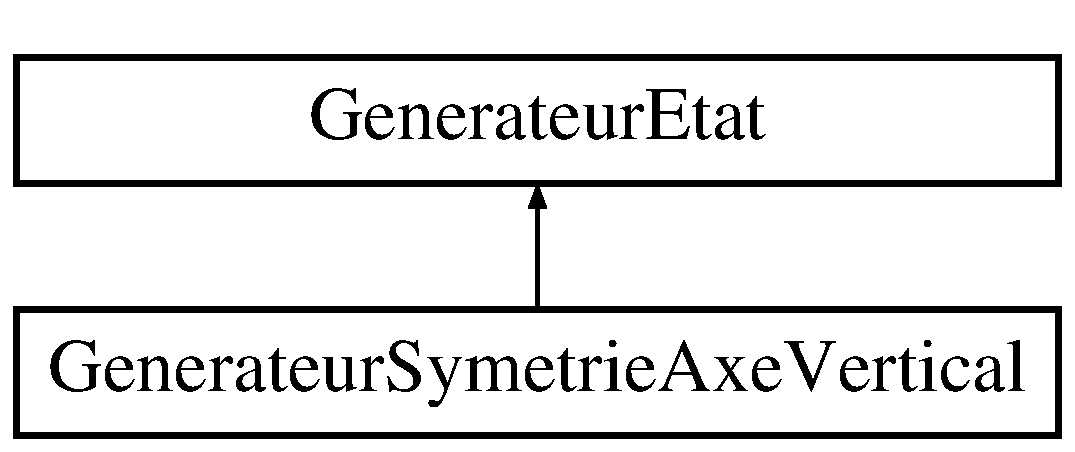
\includegraphics[height=2.000000cm]{class_generateur_symetrie_axe_vertical}
\end{center}
\end{figure}
\subsection*{Fonctions membres publiques}
\begin{DoxyCompactItemize}
\item 
\mbox{\hyperlink{class_generateur_symetrie_axe_vertical_a5e7ad0b4e452fe6a96ad75e5b54492f2}{Generateur\+Symetrie\+Axe\+Vertical}} ()=default
\item 
virtual void \mbox{\hyperlink{class_generateur_symetrie_axe_vertical_ae782046a73fc7624212c3c5988de949f}{Generer\+Etat}} (int nb\+Etats, \mbox{\hyperlink{class_etat}{Etat}} \&grille) const override
\item 
\mbox{\hyperlink{class_generateur_symetrie_axe_vertical_ae2a3a066dba020c68a91739956fb01ac}{$\sim$\+Generateur\+Symetrie\+Axe\+Vertical}} ()=default
\end{DoxyCompactItemize}


\subsection{Documentation des constructeurs et destructeur}
\mbox{\Hypertarget{class_generateur_symetrie_axe_vertical_a5e7ad0b4e452fe6a96ad75e5b54492f2}\label{class_generateur_symetrie_axe_vertical_a5e7ad0b4e452fe6a96ad75e5b54492f2}} 
\index{Generateur\+Symetrie\+Axe\+Vertical@{Generateur\+Symetrie\+Axe\+Vertical}!Generateur\+Symetrie\+Axe\+Vertical@{Generateur\+Symetrie\+Axe\+Vertical}}
\index{Generateur\+Symetrie\+Axe\+Vertical@{Generateur\+Symetrie\+Axe\+Vertical}!Generateur\+Symetrie\+Axe\+Vertical@{Generateur\+Symetrie\+Axe\+Vertical}}
\subsubsection{\texorpdfstring{Generateur\+Symetrie\+Axe\+Vertical()}{GenerateurSymetrieAxeVertical()}}
{\footnotesize\ttfamily Generateur\+Symetrie\+Axe\+Vertical\+::\+Generateur\+Symetrie\+Axe\+Vertical (\begin{DoxyParamCaption}{ }\end{DoxyParamCaption})\hspace{0.3cm}{\ttfamily [default]}}

\mbox{\Hypertarget{class_generateur_symetrie_axe_vertical_ae2a3a066dba020c68a91739956fb01ac}\label{class_generateur_symetrie_axe_vertical_ae2a3a066dba020c68a91739956fb01ac}} 
\index{Generateur\+Symetrie\+Axe\+Vertical@{Generateur\+Symetrie\+Axe\+Vertical}!````~Generateur\+Symetrie\+Axe\+Vertical@{$\sim$\+Generateur\+Symetrie\+Axe\+Vertical}}
\index{````~Generateur\+Symetrie\+Axe\+Vertical@{$\sim$\+Generateur\+Symetrie\+Axe\+Vertical}!Generateur\+Symetrie\+Axe\+Vertical@{Generateur\+Symetrie\+Axe\+Vertical}}
\subsubsection{\texorpdfstring{$\sim$\+Generateur\+Symetrie\+Axe\+Vertical()}{~GenerateurSymetrieAxeVertical()}}
{\footnotesize\ttfamily Generateur\+Symetrie\+Axe\+Vertical\+::$\sim$\+Generateur\+Symetrie\+Axe\+Vertical (\begin{DoxyParamCaption}{ }\end{DoxyParamCaption})\hspace{0.3cm}{\ttfamily [default]}}



\subsection{Documentation des fonctions membres}
\mbox{\Hypertarget{class_generateur_symetrie_axe_vertical_ae782046a73fc7624212c3c5988de949f}\label{class_generateur_symetrie_axe_vertical_ae782046a73fc7624212c3c5988de949f}} 
\index{Generateur\+Symetrie\+Axe\+Vertical@{Generateur\+Symetrie\+Axe\+Vertical}!Generer\+Etat@{Generer\+Etat}}
\index{Generer\+Etat@{Generer\+Etat}!Generateur\+Symetrie\+Axe\+Vertical@{Generateur\+Symetrie\+Axe\+Vertical}}
\subsubsection{\texorpdfstring{Generer\+Etat()}{GenererEtat()}}
{\footnotesize\ttfamily void Generateur\+Symetrie\+Axe\+Vertical\+::\+Generer\+Etat (\begin{DoxyParamCaption}\item[{int}]{nb\+Etats,  }\item[{\mbox{\hyperlink{class_etat}{Etat}} \&}]{grille }\end{DoxyParamCaption}) const\hspace{0.3cm}{\ttfamily [override]}, {\ttfamily [virtual]}}



Implémente \mbox{\hyperlink{class_generateur_etat_a0698d6706e0aaa2e597bdaf280806835}{Generateur\+Etat}}.



La documentation de cette classe a été générée à partir des fichiers suivants \+:\begin{DoxyCompactItemize}
\item 
C\+:/\+Users/maxn0/git/\+L\+O21/\+Auto\+Cell/\mbox{\hyperlink{generateuretat_8h}{generateuretat.\+h}}\item 
C\+:/\+Users/maxn0/git/\+L\+O21/\+Auto\+Cell/\mbox{\hyperlink{generateuretat_8cpp}{generateuretat.\+cpp}}\end{DoxyCompactItemize}

\hypertarget{class_etat_1_1iterator}{}\section{Référence de la classe Etat\+:\+:iterator}
\label{class_etat_1_1iterator}\index{Etat\+::iterator@{Etat\+::iterator}}


{\ttfamily \#include $<$etat.\+h$>$}

\subsection*{Fonctions membres publiques}
\begin{DoxyCompactItemize}
\item 
\mbox{\hyperlink{class_etat_1_1iterator}{iterator}} \& \mbox{\hyperlink{class_etat_1_1iterator_a7e2fe0cbe54ffc96b76aef84721d10fc}{operator++}} ()
\item 
\mbox{\hyperlink{class_cell}{Cell}} \& \mbox{\hyperlink{class_etat_1_1iterator_ab9a283bfd82bf15cac4f21422ceee680}{operator$\ast$}} () const
\item 
bool \mbox{\hyperlink{class_etat_1_1iterator_a5fd28a48c9b5ae5ccb7c3223dfcbd2da}{operator!=}} (\mbox{\hyperlink{class_etat_1_1iterator}{iterator}} it) const
\end{DoxyCompactItemize}
\subsection*{Fonctions membres privées}
\begin{DoxyCompactItemize}
\item 
\mbox{\hyperlink{class_etat_1_1iterator_a01a855525508b81c9fb934919bed65fa}{iterator}} (\mbox{\hyperlink{class_etat}{Etat}} $\ast$e)
\item 
\mbox{\hyperlink{class_etat_1_1iterator_a06e37005733f77329198c45ee1c70d3e}{iterator}} (\mbox{\hyperlink{class_etat}{Etat}} $\ast$e, int ligne, int colonne)
\item 
\mbox{\hyperlink{class_etat_1_1iterator_a6748d8aed797bb910dd9816410c2adb3}{$\sim$iterator}} ()
\end{DoxyCompactItemize}
\subsection*{Attributs privés}
\begin{DoxyCompactItemize}
\item 
\mbox{\hyperlink{class_etat}{Etat}} $\ast$ \mbox{\hyperlink{class_etat_1_1iterator_af223b227a9588b31861be17ac6aac003}{etat}}
\item 
int \mbox{\hyperlink{class_etat_1_1iterator_a6be03f617a5c2e26b1e0c5f92b7da2d9}{i}}
\item 
int \mbox{\hyperlink{class_etat_1_1iterator_a1f7dadb92cecfe5dbf0f2427a9df7977}{j}}
\end{DoxyCompactItemize}
\subsection*{Amis}
\begin{DoxyCompactItemize}
\item 
class \mbox{\hyperlink{class_etat_1_1iterator_af495e82aa15594b628d4192e8ecb688b}{Etat}}
\end{DoxyCompactItemize}


\subsection{Documentation des constructeurs et destructeur}
\mbox{\Hypertarget{class_etat_1_1iterator_a01a855525508b81c9fb934919bed65fa}\label{class_etat_1_1iterator_a01a855525508b81c9fb934919bed65fa}} 
\index{Etat\+::iterator@{Etat\+::iterator}!iterator@{iterator}}
\index{iterator@{iterator}!Etat\+::iterator@{Etat\+::iterator}}
\subsubsection{\texorpdfstring{iterator()}{iterator()}\hspace{0.1cm}{\footnotesize\ttfamily [1/2]}}
{\footnotesize\ttfamily Etat\+::iterator\+::iterator (\begin{DoxyParamCaption}\item[{\mbox{\hyperlink{class_etat}{Etat}} $\ast$}]{e }\end{DoxyParamCaption})\hspace{0.3cm}{\ttfamily [inline]}, {\ttfamily [private]}}

\mbox{\Hypertarget{class_etat_1_1iterator_a06e37005733f77329198c45ee1c70d3e}\label{class_etat_1_1iterator_a06e37005733f77329198c45ee1c70d3e}} 
\index{Etat\+::iterator@{Etat\+::iterator}!iterator@{iterator}}
\index{iterator@{iterator}!Etat\+::iterator@{Etat\+::iterator}}
\subsubsection{\texorpdfstring{iterator()}{iterator()}\hspace{0.1cm}{\footnotesize\ttfamily [2/2]}}
{\footnotesize\ttfamily Etat\+::iterator\+::iterator (\begin{DoxyParamCaption}\item[{\mbox{\hyperlink{class_etat}{Etat}} $\ast$}]{e,  }\item[{int}]{ligne,  }\item[{int}]{colonne }\end{DoxyParamCaption})\hspace{0.3cm}{\ttfamily [inline]}, {\ttfamily [private]}}

\mbox{\Hypertarget{class_etat_1_1iterator_a6748d8aed797bb910dd9816410c2adb3}\label{class_etat_1_1iterator_a6748d8aed797bb910dd9816410c2adb3}} 
\index{Etat\+::iterator@{Etat\+::iterator}!````~iterator@{$\sim$iterator}}
\index{````~iterator@{$\sim$iterator}!Etat\+::iterator@{Etat\+::iterator}}
\subsubsection{\texorpdfstring{$\sim$iterator()}{~iterator()}}
{\footnotesize\ttfamily Etat\+::iterator\+::$\sim$iterator (\begin{DoxyParamCaption}{ }\end{DoxyParamCaption})\hspace{0.3cm}{\ttfamily [inline]}, {\ttfamily [private]}}



\subsection{Documentation des fonctions membres}
\mbox{\Hypertarget{class_etat_1_1iterator_a5fd28a48c9b5ae5ccb7c3223dfcbd2da}\label{class_etat_1_1iterator_a5fd28a48c9b5ae5ccb7c3223dfcbd2da}} 
\index{Etat\+::iterator@{Etat\+::iterator}!operator"!=@{operator"!=}}
\index{operator"!=@{operator"!=}!Etat\+::iterator@{Etat\+::iterator}}
\subsubsection{\texorpdfstring{operator"!=()}{operator!=()}}
{\footnotesize\ttfamily bool Etat\+::iterator\+::operator!= (\begin{DoxyParamCaption}\item[{\mbox{\hyperlink{class_etat_1_1iterator}{iterator}}}]{it }\end{DoxyParamCaption}) const\hspace{0.3cm}{\ttfamily [inline]}}

\mbox{\Hypertarget{class_etat_1_1iterator_ab9a283bfd82bf15cac4f21422ceee680}\label{class_etat_1_1iterator_ab9a283bfd82bf15cac4f21422ceee680}} 
\index{Etat\+::iterator@{Etat\+::iterator}!operator$\ast$@{operator$\ast$}}
\index{operator$\ast$@{operator$\ast$}!Etat\+::iterator@{Etat\+::iterator}}
\subsubsection{\texorpdfstring{operator$\ast$()}{operator*()}}
{\footnotesize\ttfamily \mbox{\hyperlink{class_cell}{Cell}}\& Etat\+::iterator\+::operator$\ast$ (\begin{DoxyParamCaption}{ }\end{DoxyParamCaption}) const\hspace{0.3cm}{\ttfamily [inline]}}

\mbox{\Hypertarget{class_etat_1_1iterator_a7e2fe0cbe54ffc96b76aef84721d10fc}\label{class_etat_1_1iterator_a7e2fe0cbe54ffc96b76aef84721d10fc}} 
\index{Etat\+::iterator@{Etat\+::iterator}!operator++@{operator++}}
\index{operator++@{operator++}!Etat\+::iterator@{Etat\+::iterator}}
\subsubsection{\texorpdfstring{operator++()}{operator++()}}
{\footnotesize\ttfamily \mbox{\hyperlink{class_etat_1_1iterator}{iterator}}\& Etat\+::iterator\+::operator++ (\begin{DoxyParamCaption}{ }\end{DoxyParamCaption})\hspace{0.3cm}{\ttfamily [inline]}}



\subsection{Documentation des fonctions amies et associées}
\mbox{\Hypertarget{class_etat_1_1iterator_af495e82aa15594b628d4192e8ecb688b}\label{class_etat_1_1iterator_af495e82aa15594b628d4192e8ecb688b}} 
\index{Etat\+::iterator@{Etat\+::iterator}!Etat@{Etat}}
\index{Etat@{Etat}!Etat\+::iterator@{Etat\+::iterator}}
\subsubsection{\texorpdfstring{Etat}{Etat}}
{\footnotesize\ttfamily friend class \mbox{\hyperlink{class_etat}{Etat}}\hspace{0.3cm}{\ttfamily [friend]}}



\subsection{Documentation des données membres}
\mbox{\Hypertarget{class_etat_1_1iterator_af223b227a9588b31861be17ac6aac003}\label{class_etat_1_1iterator_af223b227a9588b31861be17ac6aac003}} 
\index{Etat\+::iterator@{Etat\+::iterator}!etat@{etat}}
\index{etat@{etat}!Etat\+::iterator@{Etat\+::iterator}}
\subsubsection{\texorpdfstring{etat}{etat}}
{\footnotesize\ttfamily \mbox{\hyperlink{class_etat}{Etat}}$\ast$ Etat\+::iterator\+::etat\hspace{0.3cm}{\ttfamily [private]}}

\mbox{\Hypertarget{class_etat_1_1iterator_a6be03f617a5c2e26b1e0c5f92b7da2d9}\label{class_etat_1_1iterator_a6be03f617a5c2e26b1e0c5f92b7da2d9}} 
\index{Etat\+::iterator@{Etat\+::iterator}!i@{i}}
\index{i@{i}!Etat\+::iterator@{Etat\+::iterator}}
\subsubsection{\texorpdfstring{i}{i}}
{\footnotesize\ttfamily int Etat\+::iterator\+::i\hspace{0.3cm}{\ttfamily [private]}}

\mbox{\Hypertarget{class_etat_1_1iterator_a1f7dadb92cecfe5dbf0f2427a9df7977}\label{class_etat_1_1iterator_a1f7dadb92cecfe5dbf0f2427a9df7977}} 
\index{Etat\+::iterator@{Etat\+::iterator}!j@{j}}
\index{j@{j}!Etat\+::iterator@{Etat\+::iterator}}
\subsubsection{\texorpdfstring{j}{j}}
{\footnotesize\ttfamily int Etat\+::iterator\+::j\hspace{0.3cm}{\ttfamily [private]}}



La documentation de cette classe a été générée à partir du fichier suivant \+:\begin{DoxyCompactItemize}
\item 
C\+:/\+Users/maxn0/git/\+L\+O21/\+Auto\+Cell/\mbox{\hyperlink{etat_8h}{etat.\+h}}\end{DoxyCompactItemize}

\hypertarget{class_main_window}{}\section{Référence de la classe Main\+Window}
\label{class_main_window}\index{Main\+Window@{Main\+Window}}


{\ttfamily \#include $<$mainwindow.\+h$>$}

Graphe d\textquotesingle{}héritage de Main\+Window\+:\begin{figure}[H]
\begin{center}
\leavevmode
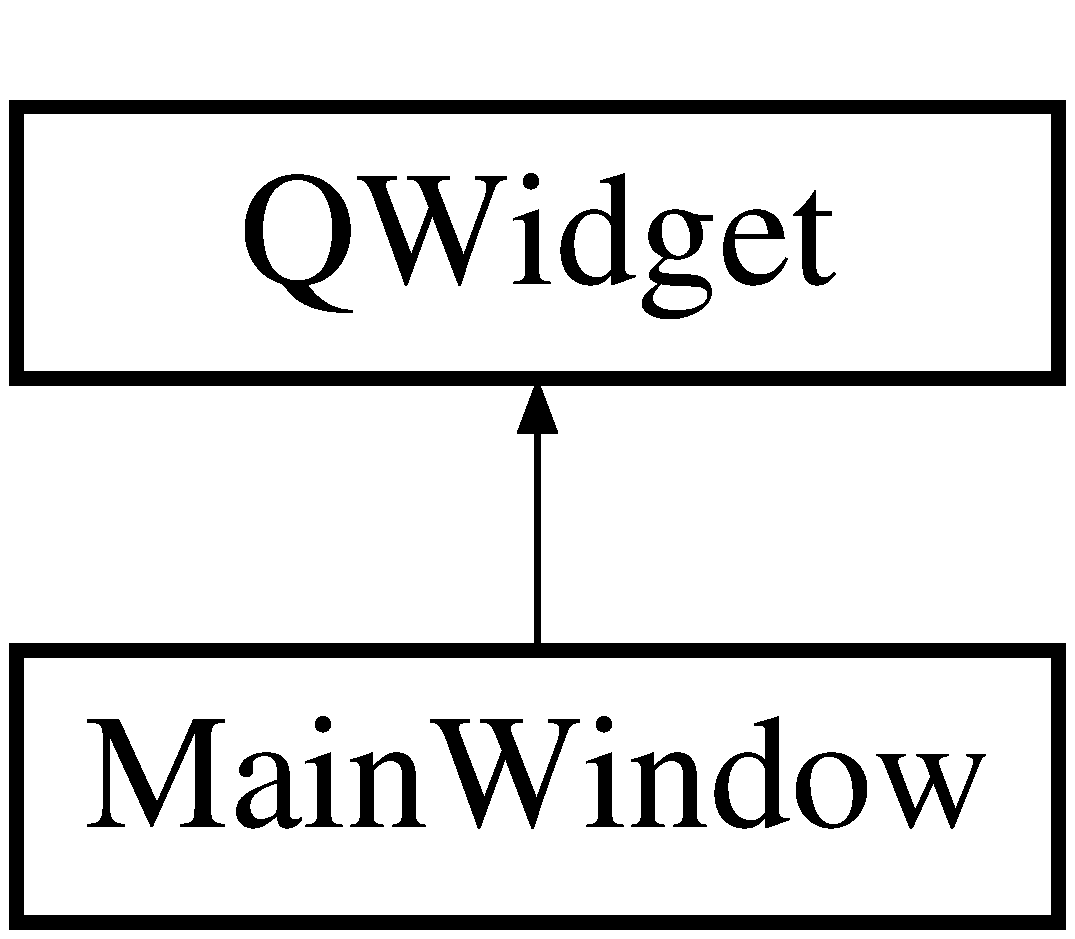
\includegraphics[height=2.000000cm]{class_main_window}
\end{center}
\end{figure}
\subsection*{Connecteurs publics}
\begin{DoxyCompactItemize}
\item 
void \mbox{\hyperlink{class_main_window_a05fb9d72c044aa3bb7d187b994704e2f}{close\+Event}} (Q\+Close\+Event $\ast$event) override
\end{DoxyCompactItemize}
\subsection*{Fonctions membres publiques}
\begin{DoxyCompactItemize}
\item 
\mbox{\hyperlink{class_main_window_a996c5a2b6f77944776856f08ec30858d}{Main\+Window}} (Q\+Widget $\ast$parent=nullptr)
\end{DoxyCompactItemize}
\subsection*{Fonctions membres privées}
\begin{DoxyCompactItemize}
\item 
void \mbox{\hyperlink{class_main_window_a2a947444fcfc921b5d237c706024891d}{load\+Config}} ()
\end{DoxyCompactItemize}
\subsection*{Attributs privés}
\begin{DoxyCompactItemize}
\item 
Q\+Combo\+Box $\ast$ \mbox{\hyperlink{class_main_window_a59a7033b41202d13e3d8a45691013147}{choix\+Dimension}}
\item 
\mbox{\hyperlink{classfenetre1_d}{fenetre1D}} $\ast$ \mbox{\hyperlink{class_main_window_a3729498370a4a7be9c5b4dad71dbe954}{dim1}}
\item 
\mbox{\hyperlink{classfenetre2_d}{fenetre2D}} $\ast$ \mbox{\hyperlink{class_main_window_a5cca01b10bb0e1ed6114418f385cb150}{dim2}}
\item 
Q\+Stacked\+Widget $\ast$ \mbox{\hyperlink{class_main_window_a825afdd9ee093af845c568d1c50de6d4}{switch\+Dim}}
\end{DoxyCompactItemize}


\subsection{Documentation des constructeurs et destructeur}
\mbox{\Hypertarget{class_main_window_a996c5a2b6f77944776856f08ec30858d}\label{class_main_window_a996c5a2b6f77944776856f08ec30858d}} 
\index{Main\+Window@{Main\+Window}!Main\+Window@{Main\+Window}}
\index{Main\+Window@{Main\+Window}!Main\+Window@{Main\+Window}}
\subsubsection{\texorpdfstring{Main\+Window()}{MainWindow()}}
{\footnotesize\ttfamily Main\+Window\+::\+Main\+Window (\begin{DoxyParamCaption}\item[{Q\+Widget $\ast$}]{parent = {\ttfamily nullptr} }\end{DoxyParamCaption})\hspace{0.3cm}{\ttfamily [explicit]}}



\subsection{Documentation des fonctions membres}
\mbox{\Hypertarget{class_main_window_a05fb9d72c044aa3bb7d187b994704e2f}\label{class_main_window_a05fb9d72c044aa3bb7d187b994704e2f}} 
\index{Main\+Window@{Main\+Window}!close\+Event@{close\+Event}}
\index{close\+Event@{close\+Event}!Main\+Window@{Main\+Window}}
\subsubsection{\texorpdfstring{close\+Event}{closeEvent}}
{\footnotesize\ttfamily void Main\+Window\+::close\+Event (\begin{DoxyParamCaption}\item[{Q\+Close\+Event $\ast$}]{event }\end{DoxyParamCaption})\hspace{0.3cm}{\ttfamily [override]}, {\ttfamily [slot]}}

\mbox{\Hypertarget{class_main_window_a2a947444fcfc921b5d237c706024891d}\label{class_main_window_a2a947444fcfc921b5d237c706024891d}} 
\index{Main\+Window@{Main\+Window}!load\+Config@{load\+Config}}
\index{load\+Config@{load\+Config}!Main\+Window@{Main\+Window}}
\subsubsection{\texorpdfstring{load\+Config()}{loadConfig()}}
{\footnotesize\ttfamily void Main\+Window\+::load\+Config (\begin{DoxyParamCaption}{ }\end{DoxyParamCaption})\hspace{0.3cm}{\ttfamily [private]}}



\subsection{Documentation des données membres}
\mbox{\Hypertarget{class_main_window_a59a7033b41202d13e3d8a45691013147}\label{class_main_window_a59a7033b41202d13e3d8a45691013147}} 
\index{Main\+Window@{Main\+Window}!choix\+Dimension@{choix\+Dimension}}
\index{choix\+Dimension@{choix\+Dimension}!Main\+Window@{Main\+Window}}
\subsubsection{\texorpdfstring{choix\+Dimension}{choixDimension}}
{\footnotesize\ttfamily Q\+Combo\+Box$\ast$ Main\+Window\+::choix\+Dimension\hspace{0.3cm}{\ttfamily [private]}}

\mbox{\Hypertarget{class_main_window_a3729498370a4a7be9c5b4dad71dbe954}\label{class_main_window_a3729498370a4a7be9c5b4dad71dbe954}} 
\index{Main\+Window@{Main\+Window}!dim1@{dim1}}
\index{dim1@{dim1}!Main\+Window@{Main\+Window}}
\subsubsection{\texorpdfstring{dim1}{dim1}}
{\footnotesize\ttfamily \mbox{\hyperlink{classfenetre1_d}{fenetre1D}}$\ast$ Main\+Window\+::dim1\hspace{0.3cm}{\ttfamily [private]}}

\mbox{\Hypertarget{class_main_window_a5cca01b10bb0e1ed6114418f385cb150}\label{class_main_window_a5cca01b10bb0e1ed6114418f385cb150}} 
\index{Main\+Window@{Main\+Window}!dim2@{dim2}}
\index{dim2@{dim2}!Main\+Window@{Main\+Window}}
\subsubsection{\texorpdfstring{dim2}{dim2}}
{\footnotesize\ttfamily \mbox{\hyperlink{classfenetre2_d}{fenetre2D}}$\ast$ Main\+Window\+::dim2\hspace{0.3cm}{\ttfamily [private]}}

\mbox{\Hypertarget{class_main_window_a825afdd9ee093af845c568d1c50de6d4}\label{class_main_window_a825afdd9ee093af845c568d1c50de6d4}} 
\index{Main\+Window@{Main\+Window}!switch\+Dim@{switch\+Dim}}
\index{switch\+Dim@{switch\+Dim}!Main\+Window@{Main\+Window}}
\subsubsection{\texorpdfstring{switch\+Dim}{switchDim}}
{\footnotesize\ttfamily Q\+Stacked\+Widget$\ast$ Main\+Window\+::switch\+Dim\hspace{0.3cm}{\ttfamily [private]}}



La documentation de cette classe a été générée à partir des fichiers suivants \+:\begin{DoxyCompactItemize}
\item 
C\+:/\+Users/maxn0/git/\+L\+O21/\+Auto\+Cell/\mbox{\hyperlink{mainwindow_8h}{mainwindow.\+h}}\item 
C\+:/\+Users/maxn0/git/\+L\+O21/\+Auto\+Cell/\mbox{\hyperlink{mainwindow_8cpp}{mainwindow.\+cpp}}\end{DoxyCompactItemize}

\hypertarget{class_moore}{}\section{Référence de la classe Moore}
\label{class_moore}\index{Moore@{Moore}}


{\ttfamily \#include $<$voisinage.\+h$>$}

Graphe d\textquotesingle{}héritage de Moore\+:\begin{figure}[H]
\begin{center}
\leavevmode
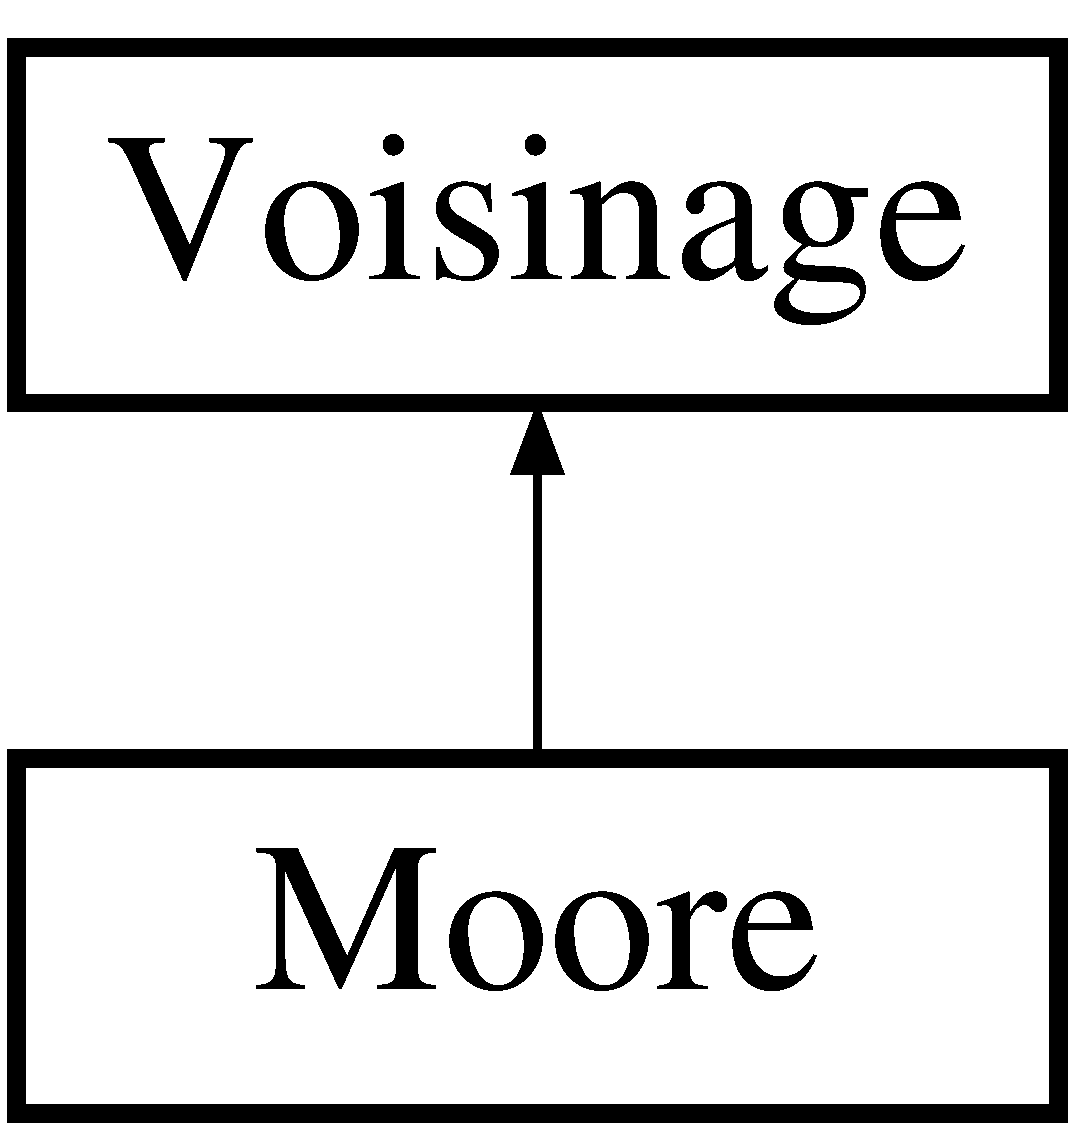
\includegraphics[height=2.000000cm]{class_moore}
\end{center}
\end{figure}
\subsection*{Fonctions membres publiques}
\begin{DoxyCompactItemize}
\item 
\mbox{\hyperlink{class_moore_a8b87d2d9c29ccbd0d8ed0081b4b58096}{Moore}} (int ordre)
\item 
\mbox{\hyperlink{class_moore_a18c2281db2524fff1559b5861cd2e3dc}{$\sim$\+Moore}} ()=default
\item 
void \mbox{\hyperlink{class_moore_a29a0a8f7b132429b5cbea4fdafcfd045}{definir\+Voisinage}} (\mbox{\hyperlink{class_etat}{Etat}} \&e) const override
\item 
std\+::string \mbox{\hyperlink{class_moore_af0398509c1540f611c000579714fbce7}{get\+Type}} () const
\end{DoxyCompactItemize}
\subsection*{Membres hérités additionnels}


\subsection{Documentation des constructeurs et destructeur}
\mbox{\Hypertarget{class_moore_a8b87d2d9c29ccbd0d8ed0081b4b58096}\label{class_moore_a8b87d2d9c29ccbd0d8ed0081b4b58096}} 
\index{Moore@{Moore}!Moore@{Moore}}
\index{Moore@{Moore}!Moore@{Moore}}
\subsubsection{\texorpdfstring{Moore()}{Moore()}}
{\footnotesize\ttfamily Moore\+::\+Moore (\begin{DoxyParamCaption}\item[{int}]{ordre }\end{DoxyParamCaption})\hspace{0.3cm}{\ttfamily [inline]}}

\mbox{\Hypertarget{class_moore_a18c2281db2524fff1559b5861cd2e3dc}\label{class_moore_a18c2281db2524fff1559b5861cd2e3dc}} 
\index{Moore@{Moore}!````~Moore@{$\sim$\+Moore}}
\index{````~Moore@{$\sim$\+Moore}!Moore@{Moore}}
\subsubsection{\texorpdfstring{$\sim$\+Moore()}{~Moore()}}
{\footnotesize\ttfamily Moore\+::$\sim$\+Moore (\begin{DoxyParamCaption}{ }\end{DoxyParamCaption})\hspace{0.3cm}{\ttfamily [default]}}



\subsection{Documentation des fonctions membres}
\mbox{\Hypertarget{class_moore_a29a0a8f7b132429b5cbea4fdafcfd045}\label{class_moore_a29a0a8f7b132429b5cbea4fdafcfd045}} 
\index{Moore@{Moore}!definir\+Voisinage@{definir\+Voisinage}}
\index{definir\+Voisinage@{definir\+Voisinage}!Moore@{Moore}}
\subsubsection{\texorpdfstring{definir\+Voisinage()}{definirVoisinage()}}
{\footnotesize\ttfamily void Moore\+::definir\+Voisinage (\begin{DoxyParamCaption}\item[{\mbox{\hyperlink{class_etat}{Etat}} \&}]{e }\end{DoxyParamCaption}) const\hspace{0.3cm}{\ttfamily [override]}, {\ttfamily [virtual]}}



Implémente \mbox{\hyperlink{class_voisinage_ac12f70bf8e971cbc8eaf8394de270d07}{Voisinage}}.

\mbox{\Hypertarget{class_moore_af0398509c1540f611c000579714fbce7}\label{class_moore_af0398509c1540f611c000579714fbce7}} 
\index{Moore@{Moore}!get\+Type@{get\+Type}}
\index{get\+Type@{get\+Type}!Moore@{Moore}}
\subsubsection{\texorpdfstring{get\+Type()}{getType()}}
{\footnotesize\ttfamily std\+::string Moore\+::get\+Type (\begin{DoxyParamCaption}{ }\end{DoxyParamCaption}) const\hspace{0.3cm}{\ttfamily [inline]}, {\ttfamily [virtual]}}



Implémente \mbox{\hyperlink{class_voisinage_a9853dfde1a68f5bb6333a8db001411a0}{Voisinage}}.



La documentation de cette classe a été générée à partir des fichiers suivants \+:\begin{DoxyCompactItemize}
\item 
C\+:/\+Users/maxn0/git/\+L\+O21/\+Auto\+Cell/\mbox{\hyperlink{voisinage_8h}{voisinage.\+h}}\item 
C\+:/\+Users/maxn0/git/\+L\+O21/\+Auto\+Cell/\mbox{\hyperlink{voisinage_8cpp}{voisinage.\+cpp}}\end{DoxyCompactItemize}

\hypertarget{class_transition_rule}{}\section{Transition\+Rule Class Reference}
\label{class_transition_rule}\index{Transition\+Rule@{Transition\+Rule}}
Inheritance diagram for Transition\+Rule\+:\begin{figure}[H]
\begin{center}
\leavevmode
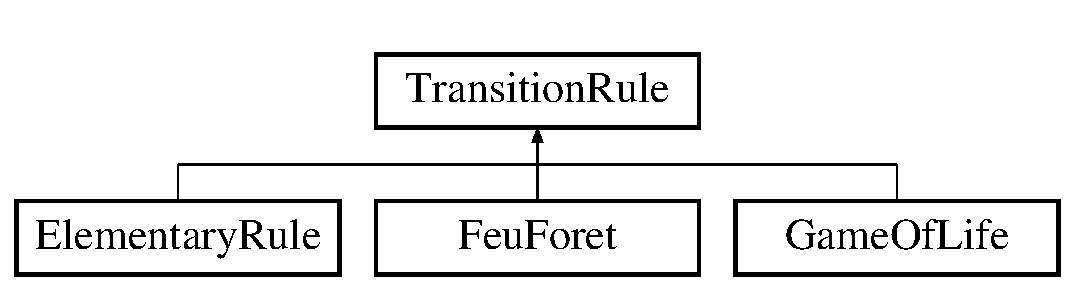
\includegraphics[height=3.000000cm]{class_transition_rule}
\end{center}
\end{figure}
\subsection*{Public Member Functions}
\begin{DoxyCompactItemize}
\item 
\mbox{\Hypertarget{class_transition_rule_a8570188a32e648ce3c08e76065f88fb7}\label{class_transition_rule_a8570188a32e648ce3c08e76065f88fb7}} 
virtual void {\bfseries Effectuer\+Transition} (\mbox{\hyperlink{class_etat}{Etat}} const \&depart, \mbox{\hyperlink{class_etat}{Etat}} \&arrivee) const
\item 
\mbox{\Hypertarget{class_transition_rule_a2b82a75ef494adc91b28755d55666e7a}\label{class_transition_rule_a2b82a75ef494adc91b28755d55666e7a}} 
virtual void {\bfseries Transition\+Cellule} (\mbox{\hyperlink{class_cell}{Cell}} const \&depart, \mbox{\hyperlink{class_cell}{Cell}} \&arrivee) const =0
\end{DoxyCompactItemize}


The documentation for this class was generated from the following files\+:\begin{DoxyCompactItemize}
\item 
C\+:/\+Users/maxn0/git/\+L\+O21/\+Auto\+Cell/transitionrule.\+h\item 
C\+:/\+Users/maxn0/git/\+L\+O21/\+Auto\+Cell/transitionrule.\+cpp\end{DoxyCompactItemize}

\hypertarget{class_voisinage}{}\section{Voisinage Class Reference}
\label{class_voisinage}\index{Voisinage@{Voisinage}}
Inheritance diagram for Voisinage\+:\begin{figure}[H]
\begin{center}
\leavevmode
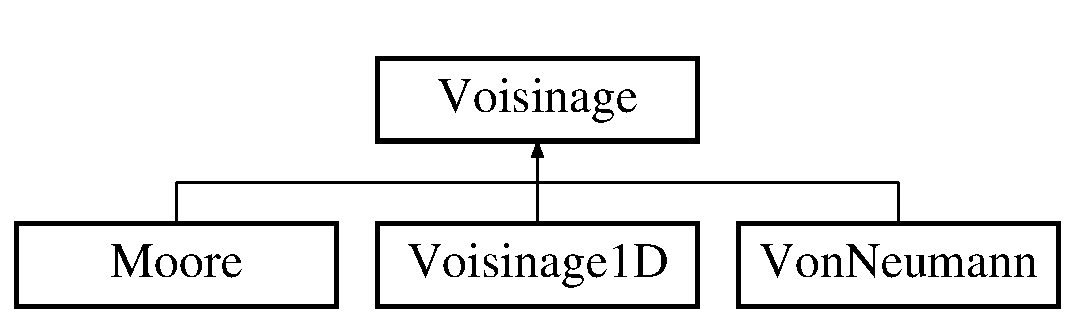
\includegraphics[height=3.000000cm]{class_voisinage}
\end{center}
\end{figure}
\subsection*{Public Member Functions}
\begin{DoxyCompactItemize}
\item 
\mbox{\Hypertarget{class_voisinage_a58416a610f5800ed165b0a68e9a78689}\label{class_voisinage_a58416a610f5800ed165b0a68e9a78689}} 
virtual void {\bfseries definir\+Voisinage} (\mbox{\hyperlink{class_etat}{Etat}} \&e, int ordre) const =0
\end{DoxyCompactItemize}


The documentation for this class was generated from the following file\+:\begin{DoxyCompactItemize}
\item 
C\+:/\+Users/maxn0/git/\+L\+O21/\+Auto\+Cell/voisinage.\+h\end{DoxyCompactItemize}

\hypertarget{class_voisinage1_d}{}\section{Référence de la classe Voisinage1D}
\label{class_voisinage1_d}\index{Voisinage1D@{Voisinage1D}}


{\ttfamily \#include $<$voisinage.\+h$>$}

Graphe d\textquotesingle{}héritage de Voisinage1D\+:\begin{figure}[H]
\begin{center}
\leavevmode
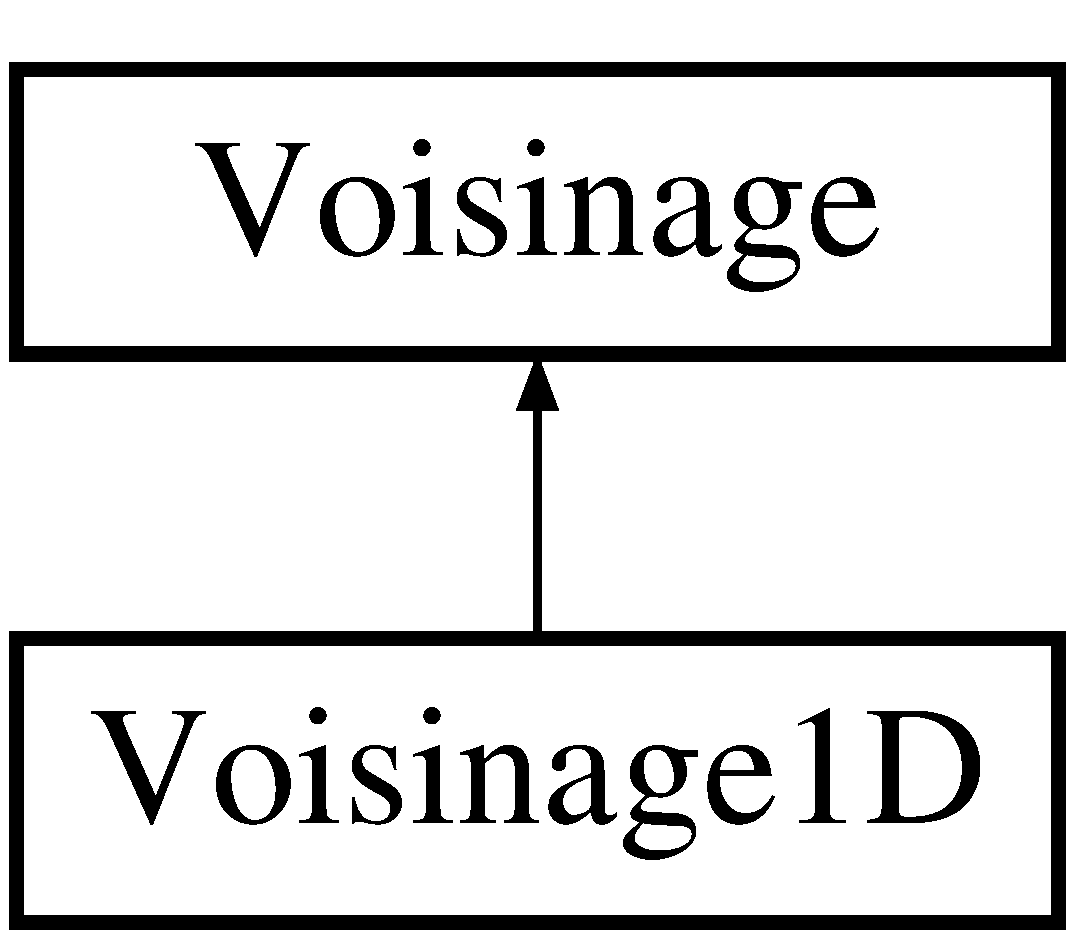
\includegraphics[height=2.000000cm]{class_voisinage1_d}
\end{center}
\end{figure}
\subsection*{Fonctions membres publiques}
\begin{DoxyCompactItemize}
\item 
\mbox{\hyperlink{class_voisinage1_d_a7077ba429224a21bc170dabcefea676e}{Voisinage1D}} (int ordre)
\item 
\mbox{\hyperlink{class_voisinage1_d_acb729fcae98b25a67d33098ef4a38260}{$\sim$\+Voisinage1D}} ()=default
\item 
void \mbox{\hyperlink{class_voisinage1_d_afdc267252af9b94fe26f5414d1472265}{definir\+Voisinage}} (\mbox{\hyperlink{class_etat}{Etat}} \&e) const final
\item 
std\+::string \mbox{\hyperlink{class_voisinage1_d_a92cc6dea76b6426d3cdaf849d18d205c}{get\+Type}} () const
\end{DoxyCompactItemize}
\subsection*{Membres hérités additionnels}


\subsection{Documentation des constructeurs et destructeur}
\mbox{\Hypertarget{class_voisinage1_d_a7077ba429224a21bc170dabcefea676e}\label{class_voisinage1_d_a7077ba429224a21bc170dabcefea676e}} 
\index{Voisinage1D@{Voisinage1D}!Voisinage1D@{Voisinage1D}}
\index{Voisinage1D@{Voisinage1D}!Voisinage1D@{Voisinage1D}}
\subsubsection{\texorpdfstring{Voisinage1\+D()}{Voisinage1D()}}
{\footnotesize\ttfamily Voisinage1\+D\+::\+Voisinage1D (\begin{DoxyParamCaption}\item[{int}]{ordre }\end{DoxyParamCaption})\hspace{0.3cm}{\ttfamily [inline]}}

\mbox{\Hypertarget{class_voisinage1_d_acb729fcae98b25a67d33098ef4a38260}\label{class_voisinage1_d_acb729fcae98b25a67d33098ef4a38260}} 
\index{Voisinage1D@{Voisinage1D}!````~Voisinage1D@{$\sim$\+Voisinage1D}}
\index{````~Voisinage1D@{$\sim$\+Voisinage1D}!Voisinage1D@{Voisinage1D}}
\subsubsection{\texorpdfstring{$\sim$\+Voisinage1\+D()}{~Voisinage1D()}}
{\footnotesize\ttfamily Voisinage1\+D\+::$\sim$\+Voisinage1D (\begin{DoxyParamCaption}{ }\end{DoxyParamCaption})\hspace{0.3cm}{\ttfamily [default]}}



\subsection{Documentation des fonctions membres}
\mbox{\Hypertarget{class_voisinage1_d_afdc267252af9b94fe26f5414d1472265}\label{class_voisinage1_d_afdc267252af9b94fe26f5414d1472265}} 
\index{Voisinage1D@{Voisinage1D}!definir\+Voisinage@{definir\+Voisinage}}
\index{definir\+Voisinage@{definir\+Voisinage}!Voisinage1D@{Voisinage1D}}
\subsubsection{\texorpdfstring{definir\+Voisinage()}{definirVoisinage()}}
{\footnotesize\ttfamily void Voisinage1\+D\+::definir\+Voisinage (\begin{DoxyParamCaption}\item[{\mbox{\hyperlink{class_etat}{Etat}} \&}]{e }\end{DoxyParamCaption}) const\hspace{0.3cm}{\ttfamily [final]}, {\ttfamily [virtual]}}



Implémente \mbox{\hyperlink{class_voisinage_ac12f70bf8e971cbc8eaf8394de270d07}{Voisinage}}.

\mbox{\Hypertarget{class_voisinage1_d_a92cc6dea76b6426d3cdaf849d18d205c}\label{class_voisinage1_d_a92cc6dea76b6426d3cdaf849d18d205c}} 
\index{Voisinage1D@{Voisinage1D}!get\+Type@{get\+Type}}
\index{get\+Type@{get\+Type}!Voisinage1D@{Voisinage1D}}
\subsubsection{\texorpdfstring{get\+Type()}{getType()}}
{\footnotesize\ttfamily std\+::string Voisinage1\+D\+::get\+Type (\begin{DoxyParamCaption}{ }\end{DoxyParamCaption}) const\hspace{0.3cm}{\ttfamily [inline]}, {\ttfamily [virtual]}}



Implémente \mbox{\hyperlink{class_voisinage_a9853dfde1a68f5bb6333a8db001411a0}{Voisinage}}.



La documentation de cette classe a été générée à partir des fichiers suivants \+:\begin{DoxyCompactItemize}
\item 
C\+:/\+Users/maxn0/git/\+L\+O21/\+Auto\+Cell/\mbox{\hyperlink{voisinage_8h}{voisinage.\+h}}\item 
C\+:/\+Users/maxn0/git/\+L\+O21/\+Auto\+Cell/\mbox{\hyperlink{voisinage_8cpp}{voisinage.\+cpp}}\end{DoxyCompactItemize}

\hypertarget{class_von_neumann}{}\section{Von\+Neumann Class Reference}
\label{class_von_neumann}\index{Von\+Neumann@{Von\+Neumann}}
Inheritance diagram for Von\+Neumann\+:\begin{figure}[H]
\begin{center}
\leavevmode
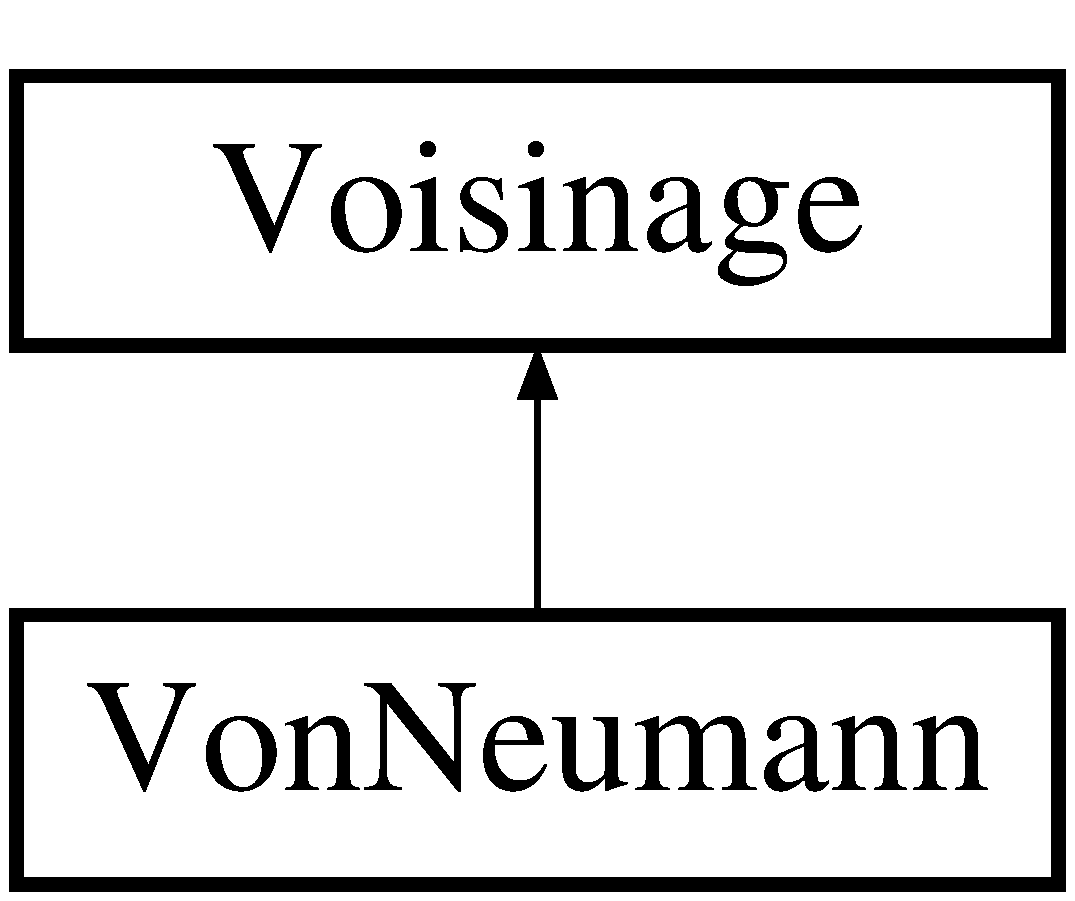
\includegraphics[height=3.000000cm]{class_von_neumann}
\end{center}
\end{figure}
\subsection*{Public Member Functions}
\begin{DoxyCompactItemize}
\item 
\mbox{\Hypertarget{class_von_neumann_a20b458d41f227a3d39f44e08376b80eb}\label{class_von_neumann_a20b458d41f227a3d39f44e08376b80eb}} 
void {\bfseries definir\+Voisinage} (\mbox{\hyperlink{class_etat}{Etat}} \&e, int ordre) const override
\end{DoxyCompactItemize}


The documentation for this class was generated from the following files\+:\begin{DoxyCompactItemize}
\item 
C\+:/\+Users/maxn0/git/\+L\+O21/\+Auto\+Cell/voisinage.\+h\item 
C\+:/\+Users/maxn0/git/\+L\+O21/\+Auto\+Cell/voisinage.\+cpp\end{DoxyCompactItemize}

\chapter{Documentation des fichiers}
\hypertarget{automateexception_8h}{}\section{C\+:/\+Users/maxn0/git/\+L\+O21/\+Auto\+Cell/automateexception.h File Reference}
\label{automateexception_8h}\index{C\+:/\+Users/maxn0/git/\+L\+O21/\+Auto\+Cell/automateexception.\+h@{C\+:/\+Users/maxn0/git/\+L\+O21/\+Auto\+Cell/automateexception.\+h}}
{\ttfamily \#include $<$string$>$}\newline
\subsection*{Classes}
\begin{DoxyCompactItemize}
\item 
class \mbox{\hyperlink{class_automate_exception}{Automate\+Exception}}
\end{DoxyCompactItemize}

\hypertarget{cabuilder_8h}{}\section{Référence du fichier C\+:/\+Users/maxn0/git/\+L\+O21/\+Auto\+Cell/cabuilder.h}
\label{cabuilder_8h}\index{C\+:/\+Users/maxn0/git/\+L\+O21/\+Auto\+Cell/cabuilder.\+h@{C\+:/\+Users/maxn0/git/\+L\+O21/\+Auto\+Cell/cabuilder.\+h}}


Déclaration des classes \mbox{\hyperlink{class_c_a_builder1_d}{C\+A\+Builder1D}} et \mbox{\hyperlink{class_c_a_builder2_d}{C\+A\+Builder2D}}.  


{\ttfamily \#include \char`\"{}cellularautomata.\+h\char`\"{}}\newline
{\ttfamily \#include $<$vector$>$}\newline
\subsection*{Classes}
\begin{DoxyCompactItemize}
\item 
class \mbox{\hyperlink{class_c_a_builder}{C\+A\+Builder}}
\begin{DoxyCompactList}\small\item\em Classe de base qui permet de construire les sous-\/parties nécessaire à la construction d\textquotesingle{}un \mbox{\hyperlink{class_cellular_automata}{Cellular\+Automata}}. \end{DoxyCompactList}\item 
class \mbox{\hyperlink{class_c_a_builder1_d}{C\+A\+Builder1D}}
\begin{DoxyCompactList}\small\item\em Classe permettant de construire toutes les sous-\/parties nécessaires à la construction d\textquotesingle{}un automate cellulaire 1D. \end{DoxyCompactList}\item 
class \mbox{\hyperlink{class_c_a_builder2_d}{C\+A\+Builder2D}}
\begin{DoxyCompactList}\small\item\em Classe permettant de construire toutes les sous-\/parties nécessaires à la construction d\textquotesingle{}un automate cellulaire 2D. \end{DoxyCompactList}\end{DoxyCompactItemize}


\subsection{Description détaillée}
Déclaration des classes \mbox{\hyperlink{class_c_a_builder1_d}{C\+A\+Builder1D}} et \mbox{\hyperlink{class_c_a_builder2_d}{C\+A\+Builder2D}}. 


\hypertarget{cell_8cpp}{}\section{Référence du fichier C\+:/\+Users/maxn0/git/\+L\+O21/\+Auto\+Cell/cell.cpp}
\label{cell_8cpp}\index{C\+:/\+Users/maxn0/git/\+L\+O21/\+Auto\+Cell/cell.\+cpp@{C\+:/\+Users/maxn0/git/\+L\+O21/\+Auto\+Cell/cell.\+cpp}}


implémentation des méthodes non inline de la classe \mbox{\hyperlink{class_cell}{Cell}}  


{\ttfamily \#include \char`\"{}cell.\+h\char`\"{}}\newline


\subsection{Description détaillée}
implémentation des méthodes non inline de la classe \mbox{\hyperlink{class_cell}{Cell}} 

\begin{DoxyVersion}{Version}
1.\+0 
\end{DoxyVersion}

\hypertarget{cell_8h}{}\section{C\+:/\+Users/maxn0/git/\+L\+O21/\+Auto\+Cell/cell.h File Reference}
\label{cell_8h}\index{C\+:/\+Users/maxn0/git/\+L\+O21/\+Auto\+Cell/cell.\+h@{C\+:/\+Users/maxn0/git/\+L\+O21/\+Auto\+Cell/cell.\+h}}
{\ttfamily \#include $<$vector$>$}\newline
{\ttfamily \#include \char`\"{}automateexception.\+h\char`\"{}}\newline
\subsection*{Classes}
\begin{DoxyCompactItemize}
\item 
class \mbox{\hyperlink{class_cell}{Cell}}
\end{DoxyCompactItemize}
\subsection*{Enumerations}
\begin{DoxyCompactItemize}
\item 
enum \mbox{\hyperlink{cell_8h_ae60adcb558b7f2142c3aa2dd94aaa535}{etat}} \{ \mbox{\hyperlink{cell_8h_ae60adcb558b7f2142c3aa2dd94aaa535a35653913ced93d8199f0378ec538a0c7}{B\+L\+A\+NC}} = 0, 
\mbox{\hyperlink{cell_8h_ae60adcb558b7f2142c3aa2dd94aaa535a59e3323a198f0162330111165caaf367}{N\+O\+IR}} = 1, 
\mbox{\hyperlink{cell_8h_ae60adcb558b7f2142c3aa2dd94aaa535a14aeed4d25cc6ce52191b46c1d73af92}{V\+E\+RT}} = 2, 
\mbox{\hyperlink{cell_8h_ae60adcb558b7f2142c3aa2dd94aaa535a92b33cebaccf73541ab06eca48a31e42}{R\+O\+U\+GE}} = 3
 \}
\end{DoxyCompactItemize}


\subsection{Enumeration Type Documentation}
\mbox{\Hypertarget{cell_8h_ae60adcb558b7f2142c3aa2dd94aaa535}\label{cell_8h_ae60adcb558b7f2142c3aa2dd94aaa535}} 
\index{cell.\+h@{cell.\+h}!etat@{etat}}
\index{etat@{etat}!cell.\+h@{cell.\+h}}
\subsubsection{\texorpdfstring{etat}{etat}}
{\footnotesize\ttfamily enum \mbox{\hyperlink{cell_8h_ae60adcb558b7f2142c3aa2dd94aaa535}{etat}}}

\begin{DoxyEnumFields}{Enumerator}
\raisebox{\heightof{T}}[0pt][0pt]{\index{B\+L\+A\+NC@{B\+L\+A\+NC}!cell.\+h@{cell.\+h}}\index{cell.\+h@{cell.\+h}!B\+L\+A\+NC@{B\+L\+A\+NC}}}\mbox{\Hypertarget{cell_8h_ae60adcb558b7f2142c3aa2dd94aaa535a35653913ced93d8199f0378ec538a0c7}\label{cell_8h_ae60adcb558b7f2142c3aa2dd94aaa535a35653913ced93d8199f0378ec538a0c7}} 
B\+L\+A\+NC&\\
\hline

\raisebox{\heightof{T}}[0pt][0pt]{\index{N\+O\+IR@{N\+O\+IR}!cell.\+h@{cell.\+h}}\index{cell.\+h@{cell.\+h}!N\+O\+IR@{N\+O\+IR}}}\mbox{\Hypertarget{cell_8h_ae60adcb558b7f2142c3aa2dd94aaa535a59e3323a198f0162330111165caaf367}\label{cell_8h_ae60adcb558b7f2142c3aa2dd94aaa535a59e3323a198f0162330111165caaf367}} 
N\+O\+IR&\\
\hline

\raisebox{\heightof{T}}[0pt][0pt]{\index{V\+E\+RT@{V\+E\+RT}!cell.\+h@{cell.\+h}}\index{cell.\+h@{cell.\+h}!V\+E\+RT@{V\+E\+RT}}}\mbox{\Hypertarget{cell_8h_ae60adcb558b7f2142c3aa2dd94aaa535a14aeed4d25cc6ce52191b46c1d73af92}\label{cell_8h_ae60adcb558b7f2142c3aa2dd94aaa535a14aeed4d25cc6ce52191b46c1d73af92}} 
V\+E\+RT&\\
\hline

\raisebox{\heightof{T}}[0pt][0pt]{\index{R\+O\+U\+GE@{R\+O\+U\+GE}!cell.\+h@{cell.\+h}}\index{cell.\+h@{cell.\+h}!R\+O\+U\+GE@{R\+O\+U\+GE}}}\mbox{\Hypertarget{cell_8h_ae60adcb558b7f2142c3aa2dd94aaa535a92b33cebaccf73541ab06eca48a31e42}\label{cell_8h_ae60adcb558b7f2142c3aa2dd94aaa535a92b33cebaccf73541ab06eca48a31e42}} 
R\+O\+U\+GE&\\
\hline

\end{DoxyEnumFields}

\hypertarget{cellularautomata_8cpp}{}\section{Référence du fichier C\+:/\+Users/maxn0/git/\+L\+O21/\+Auto\+Cell/cellularautomata.cpp}
\label{cellularautomata_8cpp}\index{C\+:/\+Users/maxn0/git/\+L\+O21/\+Auto\+Cell/cellularautomata.\+cpp@{C\+:/\+Users/maxn0/git/\+L\+O21/\+Auto\+Cell/cellularautomata.\+cpp}}
{\ttfamily \#include \char`\"{}cellularautomata.\+h\char`\"{}}\newline
{\ttfamily \#include $<$iostream$>$}\newline

\hypertarget{cellularautomata_8h}{}\section{C\+:/\+Users/maxn0/git/\+L\+O21/\+Auto\+Cell/cellularautomata.h File Reference}
\label{cellularautomata_8h}\index{C\+:/\+Users/maxn0/git/\+L\+O21/\+Auto\+Cell/cellularautomata.\+h@{C\+:/\+Users/maxn0/git/\+L\+O21/\+Auto\+Cell/cellularautomata.\+h}}
{\ttfamily \#include \char`\"{}cell.\+h\char`\"{}}\newline
{\ttfamily \#include \char`\"{}generateuretat.\+h\char`\"{}}\newline
{\ttfamily \#include \char`\"{}etat.\+h\char`\"{}}\newline
{\ttfamily \#include \char`\"{}voisinage.\+h\char`\"{}}\newline
{\ttfamily \#include \char`\"{}transitionrule.\+h\char`\"{}}\newline
\subsection*{Classes}
\begin{DoxyCompactItemize}
\item 
class \mbox{\hyperlink{class_cellular_automata}{Cellular\+Automata}}
\end{DoxyCompactItemize}

\hypertarget{etat_8cpp}{}\section{C\+:/\+Users/maxn0/git/\+L\+O21/\+Auto\+Cell/etat.cpp File Reference}
\label{etat_8cpp}\index{C\+:/\+Users/maxn0/git/\+L\+O21/\+Auto\+Cell/etat.\+cpp@{C\+:/\+Users/maxn0/git/\+L\+O21/\+Auto\+Cell/etat.\+cpp}}
{\ttfamily \#include \char`\"{}etat.\+h\char`\"{}}\newline

\hypertarget{etat_8h}{}\section{Référence du fichier C\+:/\+Users/maxn0/git/\+L\+O21/\+Auto\+Cell/etat.h}
\label{etat_8h}\index{C\+:/\+Users/maxn0/git/\+L\+O21/\+Auto\+Cell/etat.\+h@{C\+:/\+Users/maxn0/git/\+L\+O21/\+Auto\+Cell/etat.\+h}}
{\ttfamily \#include \char`\"{}cell.\+h\char`\"{}}\newline
\subsection*{Classes}
\begin{DoxyCompactItemize}
\item 
class \mbox{\hyperlink{class_etat}{Etat}}
\item 
class \mbox{\hyperlink{class_etat_1_1iterator}{Etat\+::iterator}}
\item 
class \mbox{\hyperlink{class_etat_1_1const__iterator}{Etat\+::const\+\_\+iterator}}
\end{DoxyCompactItemize}

\hypertarget{fenetre1d_8cpp}{}\section{Référence du fichier C\+:/\+Users/maxn0/git/\+L\+O21/\+Auto\+Cell/fenetre1d.cpp}
\label{fenetre1d_8cpp}\index{C\+:/\+Users/maxn0/git/\+L\+O21/\+Auto\+Cell/fenetre1d.\+cpp@{C\+:/\+Users/maxn0/git/\+L\+O21/\+Auto\+Cell/fenetre1d.\+cpp}}
{\ttfamily \#include \char`\"{}fenetre1\+D.\+h\char`\"{}}\newline
{\ttfamily \#include $<$Q\+Debug$>$}\newline

\hypertarget{fenetre1d_8h}{}\section{Référence du fichier C\+:/\+Users/maxn0/git/\+L\+O21/\+Auto\+Cell/fenetre1d.h}
\label{fenetre1d_8h}\index{C\+:/\+Users/maxn0/git/\+L\+O21/\+Auto\+Cell/fenetre1d.\+h@{C\+:/\+Users/maxn0/git/\+L\+O21/\+Auto\+Cell/fenetre1d.\+h}}
{\ttfamily \#include $<$Q\+Application$>$}\newline
{\ttfamily \#include $<$Q\+Widget$>$}\newline
{\ttfamily \#include $<$Q\+Spin\+Box$>$}\newline
{\ttfamily \#include $<$Q\+Line\+Edit$>$}\newline
{\ttfamily \#include $<$Q\+Label$>$}\newline
{\ttfamily \#include $<$Q\+Int\+Validator$>$}\newline
{\ttfamily \#include $<$Q\+String$>$}\newline
{\ttfamily \#include $<$Q\+Layout$>$}\newline
{\ttfamily \#include $<$Q\+Table\+Widget$>$}\newline
{\ttfamily \#include $<$Q\+Table\+Widget\+Item$>$}\newline
{\ttfamily \#include $<$Q\+Push\+Button$>$}\newline
{\ttfamily \#include $<$Q\+Header\+View$>$}\newline
{\ttfamily \#include $<$Q\+Combo\+Box$>$}\newline
{\ttfamily \#include $<$Q\+Stacked\+Widget$>$}\newline
{\ttfamily \#include \char`\"{}cellularautomata.\+h\char`\"{}}\newline
{\ttfamily \#include \char`\"{}automateexception.\+h\char`\"{}}\newline
{\ttfamily \#include \char`\"{}fenetreconfig.\+h\char`\"{}}\newline
{\ttfamily \#include \char`\"{}sauvegarde.\+h\char`\"{}}\newline
{\ttfamily \#include $<$Q\+Timer$>$}\newline
{\ttfamily \#include $<$Q\+Settings$>$}\newline
\subsection*{Classes}
\begin{DoxyCompactItemize}
\item 
class \mbox{\hyperlink{classfenetre1_d}{fenetre1D}}
\end{DoxyCompactItemize}

\hypertarget{fenetre2d_8cpp}{}\section{Référence du fichier C\+:/\+Users/maxn0/git/\+L\+O21/\+Auto\+Cell/fenetre2d.cpp}
\label{fenetre2d_8cpp}\index{C\+:/\+Users/maxn0/git/\+L\+O21/\+Auto\+Cell/fenetre2d.\+cpp@{C\+:/\+Users/maxn0/git/\+L\+O21/\+Auto\+Cell/fenetre2d.\+cpp}}
{\ttfamily \#include \char`\"{}fenetre2\+D.\+h\char`\"{}}\newline

\hypertarget{fenetre2d_8h}{}\section{Référence du fichier C\+:/\+Users/maxn0/git/\+L\+O21/\+Auto\+Cell/fenetre2d.h}
\label{fenetre2d_8h}\index{C\+:/\+Users/maxn0/git/\+L\+O21/\+Auto\+Cell/fenetre2d.\+h@{C\+:/\+Users/maxn0/git/\+L\+O21/\+Auto\+Cell/fenetre2d.\+h}}
{\ttfamily \#include $<$Q\+Application$>$}\newline
{\ttfamily \#include $<$Q\+Widget$>$}\newline
{\ttfamily \#include $<$Q\+Spin\+Box$>$}\newline
{\ttfamily \#include $<$Q\+Line\+Edit$>$}\newline
{\ttfamily \#include $<$Q\+Label$>$}\newline
{\ttfamily \#include $<$Q\+Int\+Validator$>$}\newline
{\ttfamily \#include $<$Q\+String$>$}\newline
{\ttfamily \#include $<$Q\+Layout$>$}\newline
{\ttfamily \#include $<$Q\+Table\+Widget$>$}\newline
{\ttfamily \#include $<$Q\+Table\+Widget\+Item$>$}\newline
{\ttfamily \#include $<$Q\+Push\+Button$>$}\newline
{\ttfamily \#include $<$Q\+Header\+View$>$}\newline
{\ttfamily \#include $<$Q\+Combo\+Box$>$}\newline
{\ttfamily \#include $<$Q\+Stacked\+Widget$>$}\newline
{\ttfamily \#include \char`\"{}cellularautomata.\+h\char`\"{}}\newline
{\ttfamily \#include \char`\"{}automateexception.\+h\char`\"{}}\newline
{\ttfamily \#include \char`\"{}fenetreconfig.\+h\char`\"{}}\newline
{\ttfamily \#include \char`\"{}sauvegarde.\+h\char`\"{}}\newline
{\ttfamily \#include $<$Q\+Timer$>$}\newline
{\ttfamily \#include $<$Q\+Desktop\+Widget$>$}\newline
{\ttfamily \#include $<$Q\+Settings$>$}\newline
{\ttfamily \#include $<$sstream$>$}\newline
\subsection*{Classes}
\begin{DoxyCompactItemize}
\item 
class \mbox{\hyperlink{classfenetre2_d}{fenetre2D}}
\end{DoxyCompactItemize}

\hypertarget{fenetreconfig_8cpp}{}\section{Référence du fichier C\+:/\+Users/maxn0/git/\+L\+O21/\+Auto\+Cell/fenetreconfig.cpp}
\label{fenetreconfig_8cpp}\index{C\+:/\+Users/maxn0/git/\+L\+O21/\+Auto\+Cell/fenetreconfig.\+cpp@{C\+:/\+Users/maxn0/git/\+L\+O21/\+Auto\+Cell/fenetreconfig.\+cpp}}
{\ttfamily \#include \char`\"{}fenetreconfig.\+h\char`\"{}}\newline
{\ttfamily \#include \char`\"{}fichier.\+h\char`\"{}}\newline
\subsection*{Fonctions}
\begin{DoxyCompactItemize}
\item 
unsigned int \mbox{\hyperlink{fenetreconfig_8cpp_af04728d84267736942106ac7bda1a774}{puissance}} (unsigned int a, unsigned int b)
\end{DoxyCompactItemize}


\subsection{Documentation des fonctions}
\mbox{\Hypertarget{fenetreconfig_8cpp_af04728d84267736942106ac7bda1a774}\label{fenetreconfig_8cpp_af04728d84267736942106ac7bda1a774}} 
\index{fenetreconfig.\+cpp@{fenetreconfig.\+cpp}!puissance@{puissance}}
\index{puissance@{puissance}!fenetreconfig.\+cpp@{fenetreconfig.\+cpp}}
\subsubsection{\texorpdfstring{puissance()}{puissance()}}
{\footnotesize\ttfamily unsigned int puissance (\begin{DoxyParamCaption}\item[{unsigned int}]{a,  }\item[{unsigned int}]{b }\end{DoxyParamCaption})}


\hypertarget{fenetreconfig_8h}{}\section{Référence du fichier C\+:/\+Users/maxn0/git/\+L\+O21/\+Auto\+Cell/fenetreconfig.h}
\label{fenetreconfig_8h}\index{C\+:/\+Users/maxn0/git/\+L\+O21/\+Auto\+Cell/fenetreconfig.\+h@{C\+:/\+Users/maxn0/git/\+L\+O21/\+Auto\+Cell/fenetreconfig.\+h}}
{\ttfamily \#include $<$Q\+Widget$>$}\newline
{\ttfamily \#include $<$Q\+Spin\+Box$>$}\newline
{\ttfamily \#include $<$Q\+Line\+Edit$>$}\newline
{\ttfamily \#include $<$Q\+Reg\+Exp\+Validator$>$}\newline
{\ttfamily \#include $<$Q\+Plain\+Text\+Edit$>$}\newline
{\ttfamily \#include $<$Q\+Form\+Layout$>$}\newline
{\ttfamily \#include $<$Q\+V\+Box\+Layout$>$}\newline
{\ttfamily \#include $<$Q\+Message\+Box$>$}\newline
{\ttfamily \#include $<$Q\+Label$>$}\newline
{\ttfamily \#include $<$Q\+Combo\+Box$>$}\newline
{\ttfamily \#include $<$sstream$>$}\newline
{\ttfamily \#include $<$Q\+Settings$>$}\newline
{\ttfamily \#include \char`\"{}cabuilder.\+h\char`\"{}}\newline
\subsection*{Classes}
\begin{DoxyCompactItemize}
\item 
class \mbox{\hyperlink{classfenetre_config}{fenetre\+Config}}
\item 
class \mbox{\hyperlink{classfenetre_elementary_rule}{fenetre\+Elementary\+Rule}}
\item 
class \mbox{\hyperlink{classfenetre_game_of_life}{fenetre\+Game\+Of\+Life}}
\item 
class \mbox{\hyperlink{classfenetre_feu_foret}{fenetre\+Feu\+Foret}}
\end{DoxyCompactItemize}
\subsection*{Fonctions}
\begin{DoxyCompactItemize}
\item 
unsigned int \mbox{\hyperlink{fenetreconfig_8h_af04728d84267736942106ac7bda1a774}{puissance}} (unsigned int a, unsigned int b)
\end{DoxyCompactItemize}


\subsection{Documentation des fonctions}
\mbox{\Hypertarget{fenetreconfig_8h_af04728d84267736942106ac7bda1a774}\label{fenetreconfig_8h_af04728d84267736942106ac7bda1a774}} 
\index{fenetreconfig.\+h@{fenetreconfig.\+h}!puissance@{puissance}}
\index{puissance@{puissance}!fenetreconfig.\+h@{fenetreconfig.\+h}}
\subsubsection{\texorpdfstring{puissance()}{puissance()}}
{\footnotesize\ttfamily unsigned int puissance (\begin{DoxyParamCaption}\item[{unsigned int}]{a,  }\item[{unsigned int}]{b }\end{DoxyParamCaption})}


\hypertarget{fichier_8cpp}{}\section{Référence du fichier C\+:/\+Users/maxn0/git/\+L\+O21/\+Auto\+Cell/fichier.cpp}
\label{fichier_8cpp}\index{C\+:/\+Users/maxn0/git/\+L\+O21/\+Auto\+Cell/fichier.\+cpp@{C\+:/\+Users/maxn0/git/\+L\+O21/\+Auto\+Cell/fichier.\+cpp}}
{\ttfamily \#include \char`\"{}fichier.\+h\char`\"{}}\newline
{\ttfamily \#include $<$Q\+Debug$>$}\newline
{\ttfamily \#include $<$Q\+Message\+Box$>$}\newline

\hypertarget{fichier_8h}{}\section{Référence du fichier C\+:/\+Users/maxn0/git/\+L\+O21/\+Auto\+Cell/fichier.h}
\label{fichier_8h}\index{C\+:/\+Users/maxn0/git/\+L\+O21/\+Auto\+Cell/fichier.\+h@{C\+:/\+Users/maxn0/git/\+L\+O21/\+Auto\+Cell/fichier.\+h}}
{\ttfamily \#include $<$iostream$>$}\newline
{\ttfamily \#include $<$fstream$>$}\newline
{\ttfamily \#include $<$vector$>$}\newline
{\ttfamily \#include $<$Q\+Message\+Box$>$}\newline
{\ttfamily \#include \char`\"{}cellularautomata.\+h\char`\"{}}\newline
{\ttfamily \#include \char`\"{}cabuilder.\+h\char`\"{}}\newline
{\ttfamily \#include \char`\"{}fenetre1d.\+h\char`\"{}}\newline
{\ttfamily \#include \char`\"{}fenetre2d.\+h\char`\"{}}\newline
\subsection*{Classes}
\begin{DoxyCompactItemize}
\item 
class \mbox{\hyperlink{classfichier}{fichier}}
\item 
class \mbox{\hyperlink{classfichier_etat1_d}{fichier\+Etat1D}}
\item 
class \mbox{\hyperlink{classfichier_etat2_d}{fichier\+Etat2D}}
\item 
class \mbox{\hyperlink{classfichier_config1_d}{fichier\+Config1D}}
\item 
class \mbox{\hyperlink{classfichier_config2_d}{fichier\+Config2D}}
\end{DoxyCompactItemize}
\subsection*{Macros}
\begin{DoxyCompactItemize}
\item 
\#define \mbox{\hyperlink{fichier_8h_a007bac9cc84e5ae1b6ecf856fc27b607}{T\+A\+I\+L\+L\+E\+\_\+\+B\+UF}}~100
\end{DoxyCompactItemize}


\subsection{Documentation des macros}
\mbox{\Hypertarget{fichier_8h_a007bac9cc84e5ae1b6ecf856fc27b607}\label{fichier_8h_a007bac9cc84e5ae1b6ecf856fc27b607}} 
\index{fichier.\+h@{fichier.\+h}!T\+A\+I\+L\+L\+E\+\_\+\+B\+UF@{T\+A\+I\+L\+L\+E\+\_\+\+B\+UF}}
\index{T\+A\+I\+L\+L\+E\+\_\+\+B\+UF@{T\+A\+I\+L\+L\+E\+\_\+\+B\+UF}!fichier.\+h@{fichier.\+h}}
\subsubsection{\texorpdfstring{T\+A\+I\+L\+L\+E\+\_\+\+B\+UF}{TAILLE\_BUF}}
{\footnotesize\ttfamily \#define T\+A\+I\+L\+L\+E\+\_\+\+B\+UF~100}


\hypertarget{generateuretat_8cpp}{}\section{C\+:/\+Users/maxn0/git/\+L\+O21/\+Auto\+Cell/generateuretat.cpp File Reference}
\label{generateuretat_8cpp}\index{C\+:/\+Users/maxn0/git/\+L\+O21/\+Auto\+Cell/generateuretat.\+cpp@{C\+:/\+Users/maxn0/git/\+L\+O21/\+Auto\+Cell/generateuretat.\+cpp}}
{\ttfamily \#include \char`\"{}generateuretat.\+h\char`\"{}}\newline

\hypertarget{generateuretat_8h}{}\section{C\+:/\+Users/maxn0/git/\+L\+O21/\+Auto\+Cell/generateuretat.h File Reference}
\label{generateuretat_8h}\index{C\+:/\+Users/maxn0/git/\+L\+O21/\+Auto\+Cell/generateuretat.\+h@{C\+:/\+Users/maxn0/git/\+L\+O21/\+Auto\+Cell/generateuretat.\+h}}
{\ttfamily \#include \char`\"{}cell.\+h\char`\"{}}\newline
{\ttfamily \#include $<$vector$>$}\newline
{\ttfamily \#include $<$cstdlib$>$}\newline
{\ttfamily \#include $<$ctime$>$}\newline
{\ttfamily \#include $<$iostream$>$}\newline
\subsection*{Classes}
\begin{DoxyCompactItemize}
\item 
class \mbox{\hyperlink{class_generateur_etat}{Generateur\+Etat}}
\item 
class \mbox{\hyperlink{class_generateur_random}{Generateur\+Random}}
\item 
class \mbox{\hyperlink{class_generateur_symetrie_axe_largeur}{Generateur\+Symetrie\+Axe\+Largeur}}
\end{DoxyCompactItemize}

\hypertarget{main_8cpp}{}\section{Référence du fichier C\+:/\+Users/maxn0/git/\+L\+O21/\+Auto\+Cell/main.cpp}
\label{main_8cpp}\index{C\+:/\+Users/maxn0/git/\+L\+O21/\+Auto\+Cell/main.\+cpp@{C\+:/\+Users/maxn0/git/\+L\+O21/\+Auto\+Cell/main.\+cpp}}
{\ttfamily \#include $<$iostream$>$}\newline
{\ttfamily \#include $<$Q\+Application$>$}\newline
{\ttfamily \#include \char`\"{}cell.\+h\char`\"{}}\newline
{\ttfamily \#include \char`\"{}generateuretat.\+h\char`\"{}}\newline
{\ttfamily \#include \char`\"{}etat.\+h\char`\"{}}\newline
{\ttfamily \#include \char`\"{}voisinage.\+h\char`\"{}}\newline
{\ttfamily \#include \char`\"{}transitionrule.\+h\char`\"{}}\newline
{\ttfamily \#include \char`\"{}cellularautomata.\+h\char`\"{}}\newline
{\ttfamily \#include \char`\"{}sauvegarde.\+h\char`\"{}}\newline
{\ttfamily \#include \char`\"{}mainwindow.\+h\char`\"{}}\newline
{\ttfamily \#include $<$ctime$>$}\newline
\subsection*{Fonctions}
\begin{DoxyCompactItemize}
\item 
int \mbox{\hyperlink{main_8cpp_a0ddf1224851353fc92bfbff6f499fa97}{main}} (int argc, char $\ast$argv\mbox{[}$\,$\mbox{]})
\end{DoxyCompactItemize}


\subsection{Documentation des fonctions}
\mbox{\Hypertarget{main_8cpp_a0ddf1224851353fc92bfbff6f499fa97}\label{main_8cpp_a0ddf1224851353fc92bfbff6f499fa97}} 
\index{main.\+cpp@{main.\+cpp}!main@{main}}
\index{main@{main}!main.\+cpp@{main.\+cpp}}
\subsubsection{\texorpdfstring{main()}{main()}}
{\footnotesize\ttfamily int main (\begin{DoxyParamCaption}\item[{int}]{argc,  }\item[{char $\ast$}]{argv\mbox{[}$\,$\mbox{]} }\end{DoxyParamCaption})}


\hypertarget{mainwindow_8cpp}{}\section{Référence du fichier C\+:/\+Users/maxn0/git/\+L\+O21/\+Auto\+Cell/mainwindow.cpp}
\label{mainwindow_8cpp}\index{C\+:/\+Users/maxn0/git/\+L\+O21/\+Auto\+Cell/mainwindow.\+cpp@{C\+:/\+Users/maxn0/git/\+L\+O21/\+Auto\+Cell/mainwindow.\+cpp}}
{\ttfamily \#include \char`\"{}mainwindow.\+h\char`\"{}}\newline

\hypertarget{mainwindow_8h}{}\section{Référence du fichier C\+:/\+Users/maxn0/git/\+L\+O21/\+Auto\+Cell/mainwindow.h}
\label{mainwindow_8h}\index{C\+:/\+Users/maxn0/git/\+L\+O21/\+Auto\+Cell/mainwindow.\+h@{C\+:/\+Users/maxn0/git/\+L\+O21/\+Auto\+Cell/mainwindow.\+h}}
{\ttfamily \#include \char`\"{}fenetre1d.\+h\char`\"{}}\newline
{\ttfamily \#include \char`\"{}fenetre2d.\+h\char`\"{}}\newline
{\ttfamily \#include $<$Q\+Widget$>$}\newline
{\ttfamily \#include $<$Q\+Stacked\+Widget$>$}\newline
{\ttfamily \#include $<$Q\+Combo\+Box$>$}\newline
{\ttfamily \#include $<$Q\+Settings$>$}\newline
\subsection*{Classes}
\begin{DoxyCompactItemize}
\item 
class \mbox{\hyperlink{class_main_window}{Main\+Window}}
\end{DoxyCompactItemize}

\hypertarget{sauvegarde_8cpp}{}\section{Référence du fichier C\+:/\+Users/maxn0/git/\+L\+O21/\+Auto\+Cell/sauvegarde.cpp}
\label{sauvegarde_8cpp}\index{C\+:/\+Users/maxn0/git/\+L\+O21/\+Auto\+Cell/sauvegarde.\+cpp@{C\+:/\+Users/maxn0/git/\+L\+O21/\+Auto\+Cell/sauvegarde.\+cpp}}
{\ttfamily \#include \char`\"{}sauvegarde.\+h\char`\"{}}\newline
{\ttfamily \#include $<$Q\+Debug$>$}\newline
\subsection*{Fonctions}
\begin{DoxyCompactItemize}
\item 
bool \mbox{\hyperlink{sauvegarde_8cpp_a9d16542dcc8a340e36e363d5a3fa1a88}{sauvegarde}} (const \mbox{\hyperlink{class_cellular_automata}{Cellular\+Automata}} \&automate, \mbox{\hyperlink{sauvegarde_8h_af4bf09862c0294e937b809406a59c306}{Type\+Fichier}} t, \mbox{\hyperlink{sauvegarde_8h_ac723b01a0252e3ef0c19e62167fee796}{Dim\+Type}} d)
\item 
bool \mbox{\hyperlink{sauvegarde_8cpp_a1c2fd1001592255e8b3f9a7a3108519f}{chargement}} (const \mbox{\hyperlink{class_cellular_automata}{Cellular\+Automata}} \&automate, \mbox{\hyperlink{sauvegarde_8h_af4bf09862c0294e937b809406a59c306}{Type\+Fichier}} t, \mbox{\hyperlink{sauvegarde_8h_ac723b01a0252e3ef0c19e62167fee796}{Dim\+Type}} d)
\end{DoxyCompactItemize}


\subsection{Documentation des fonctions}
\mbox{\Hypertarget{sauvegarde_8cpp_a1c2fd1001592255e8b3f9a7a3108519f}\label{sauvegarde_8cpp_a1c2fd1001592255e8b3f9a7a3108519f}} 
\index{sauvegarde.\+cpp@{sauvegarde.\+cpp}!chargement@{chargement}}
\index{chargement@{chargement}!sauvegarde.\+cpp@{sauvegarde.\+cpp}}
\subsubsection{\texorpdfstring{chargement()}{chargement()}}
{\footnotesize\ttfamily bool chargement (\begin{DoxyParamCaption}\item[{const \mbox{\hyperlink{class_cellular_automata}{Cellular\+Automata}} \&}]{automate,  }\item[{\mbox{\hyperlink{sauvegarde_8h_af4bf09862c0294e937b809406a59c306}{Type\+Fichier}}}]{t,  }\item[{\mbox{\hyperlink{sauvegarde_8h_ac723b01a0252e3ef0c19e62167fee796}{Dim\+Type}}}]{d }\end{DoxyParamCaption})}

\mbox{\Hypertarget{sauvegarde_8cpp_a9d16542dcc8a340e36e363d5a3fa1a88}\label{sauvegarde_8cpp_a9d16542dcc8a340e36e363d5a3fa1a88}} 
\index{sauvegarde.\+cpp@{sauvegarde.\+cpp}!sauvegarde@{sauvegarde}}
\index{sauvegarde@{sauvegarde}!sauvegarde.\+cpp@{sauvegarde.\+cpp}}
\subsubsection{\texorpdfstring{sauvegarde()}{sauvegarde()}}
{\footnotesize\ttfamily bool sauvegarde (\begin{DoxyParamCaption}\item[{const \mbox{\hyperlink{class_cellular_automata}{Cellular\+Automata}} \&}]{automate,  }\item[{\mbox{\hyperlink{sauvegarde_8h_af4bf09862c0294e937b809406a59c306}{Type\+Fichier}}}]{t,  }\item[{\mbox{\hyperlink{sauvegarde_8h_ac723b01a0252e3ef0c19e62167fee796}{Dim\+Type}}}]{d }\end{DoxyParamCaption})}


\hypertarget{sauvegarde_8h}{}\section{Référence du fichier C\+:/\+Users/maxn0/git/\+L\+O21/\+Auto\+Cell/sauvegarde.h}
\label{sauvegarde_8h}\index{C\+:/\+Users/maxn0/git/\+L\+O21/\+Auto\+Cell/sauvegarde.\+h@{C\+:/\+Users/maxn0/git/\+L\+O21/\+Auto\+Cell/sauvegarde.\+h}}
{\ttfamily \#include $<$Q\+Object$>$}\newline
{\ttfamily \#include $<$Q\+Widget$>$}\newline
{\ttfamily \#include $<$Q\+Push\+Button$>$}\newline
{\ttfamily \#include $<$Q\+H\+Box\+Layout$>$}\newline
{\ttfamily \#include $<$Q\+V\+Box\+Layout$>$}\newline
{\ttfamily \#include $<$Q\+Label$>$}\newline
{\ttfamily \#include $<$Q\+Line\+Edit$>$}\newline
{\ttfamily \#include $<$Q\+File\+Dialog$>$}\newline
{\ttfamily \#include $<$Q\+Message\+Box$>$}\newline
{\ttfamily \#include $<$Q\+String$>$}\newline
{\ttfamily \#include \char`\"{}cellularautomata.\+h\char`\"{}}\newline
{\ttfamily \#include \char`\"{}fichier.\+h\char`\"{}}\newline
{\ttfamily \#include \char`\"{}fenetre1d.\+h\char`\"{}}\newline
{\ttfamily \#include \char`\"{}fenetre2d.\+h\char`\"{}}\newline
\subsection*{Énumérations}
\begin{DoxyCompactItemize}
\item 
enum \mbox{\hyperlink{sauvegarde_8h_af4bf09862c0294e937b809406a59c306}{Type\+Fichier}} \{ \mbox{\hyperlink{sauvegarde_8h_af4bf09862c0294e937b809406a59c306a228c7d5226de3d46b87bb264578e9c96}{E\+T\+AT}}, 
\mbox{\hyperlink{sauvegarde_8h_af4bf09862c0294e937b809406a59c306a702582f7f825ca83bdb076b15b4c0fc2}{C\+O\+N\+F\+IG}}
 \}
\item 
enum \mbox{\hyperlink{sauvegarde_8h_ac723b01a0252e3ef0c19e62167fee796}{Dim\+Type}} \{ \mbox{\hyperlink{sauvegarde_8h_ac723b01a0252e3ef0c19e62167fee796a0fd85b1345d8b71b3b76e8101980f618}{\+\_\+1D}}, 
\mbox{\hyperlink{sauvegarde_8h_ac723b01a0252e3ef0c19e62167fee796acff98fc949954b753f7077705091c8ee}{\+\_\+2D}}
 \}
\end{DoxyCompactItemize}
\subsection*{Fonctions}
\begin{DoxyCompactItemize}
\item 
bool \mbox{\hyperlink{sauvegarde_8h_a9d16542dcc8a340e36e363d5a3fa1a88}{sauvegarde}} (const \mbox{\hyperlink{class_cellular_automata}{Cellular\+Automata}} \&automate, \mbox{\hyperlink{sauvegarde_8h_af4bf09862c0294e937b809406a59c306}{Type\+Fichier}} t, \mbox{\hyperlink{sauvegarde_8h_ac723b01a0252e3ef0c19e62167fee796}{Dim\+Type}} d)
\item 
bool \mbox{\hyperlink{sauvegarde_8h_a1c2fd1001592255e8b3f9a7a3108519f}{chargement}} (const \mbox{\hyperlink{class_cellular_automata}{Cellular\+Automata}} \&automate, \mbox{\hyperlink{sauvegarde_8h_af4bf09862c0294e937b809406a59c306}{Type\+Fichier}} t, \mbox{\hyperlink{sauvegarde_8h_ac723b01a0252e3ef0c19e62167fee796}{Dim\+Type}} d)
\end{DoxyCompactItemize}


\subsection{Documentation du type de l\textquotesingle{}énumération}
\mbox{\Hypertarget{sauvegarde_8h_ac723b01a0252e3ef0c19e62167fee796}\label{sauvegarde_8h_ac723b01a0252e3ef0c19e62167fee796}} 
\index{sauvegarde.\+h@{sauvegarde.\+h}!Dim\+Type@{Dim\+Type}}
\index{Dim\+Type@{Dim\+Type}!sauvegarde.\+h@{sauvegarde.\+h}}
\subsubsection{\texorpdfstring{Dim\+Type}{DimType}}
{\footnotesize\ttfamily enum \mbox{\hyperlink{sauvegarde_8h_ac723b01a0252e3ef0c19e62167fee796}{Dim\+Type}}}

\begin{DoxyEnumFields}{Valeurs énumérées}
\raisebox{\heightof{T}}[0pt][0pt]{\index{\+\_\+1D@{\+\_\+1D}!sauvegarde.\+h@{sauvegarde.\+h}}\index{sauvegarde.\+h@{sauvegarde.\+h}!\+\_\+1D@{\+\_\+1D}}}\mbox{\Hypertarget{sauvegarde_8h_ac723b01a0252e3ef0c19e62167fee796a0fd85b1345d8b71b3b76e8101980f618}\label{sauvegarde_8h_ac723b01a0252e3ef0c19e62167fee796a0fd85b1345d8b71b3b76e8101980f618}} 
\+\_\+1D&\\
\hline

\raisebox{\heightof{T}}[0pt][0pt]{\index{\+\_\+2D@{\+\_\+2D}!sauvegarde.\+h@{sauvegarde.\+h}}\index{sauvegarde.\+h@{sauvegarde.\+h}!\+\_\+2D@{\+\_\+2D}}}\mbox{\Hypertarget{sauvegarde_8h_ac723b01a0252e3ef0c19e62167fee796acff98fc949954b753f7077705091c8ee}\label{sauvegarde_8h_ac723b01a0252e3ef0c19e62167fee796acff98fc949954b753f7077705091c8ee}} 
\+\_\+2D&\\
\hline

\end{DoxyEnumFields}
\mbox{\Hypertarget{sauvegarde_8h_af4bf09862c0294e937b809406a59c306}\label{sauvegarde_8h_af4bf09862c0294e937b809406a59c306}} 
\index{sauvegarde.\+h@{sauvegarde.\+h}!Type\+Fichier@{Type\+Fichier}}
\index{Type\+Fichier@{Type\+Fichier}!sauvegarde.\+h@{sauvegarde.\+h}}
\subsubsection{\texorpdfstring{Type\+Fichier}{TypeFichier}}
{\footnotesize\ttfamily enum \mbox{\hyperlink{sauvegarde_8h_af4bf09862c0294e937b809406a59c306}{Type\+Fichier}}}

\begin{DoxyEnumFields}{Valeurs énumérées}
\raisebox{\heightof{T}}[0pt][0pt]{\index{E\+T\+AT@{E\+T\+AT}!sauvegarde.\+h@{sauvegarde.\+h}}\index{sauvegarde.\+h@{sauvegarde.\+h}!E\+T\+AT@{E\+T\+AT}}}\mbox{\Hypertarget{sauvegarde_8h_af4bf09862c0294e937b809406a59c306a228c7d5226de3d46b87bb264578e9c96}\label{sauvegarde_8h_af4bf09862c0294e937b809406a59c306a228c7d5226de3d46b87bb264578e9c96}} 
E\+T\+AT&\\
\hline

\raisebox{\heightof{T}}[0pt][0pt]{\index{C\+O\+N\+F\+IG@{C\+O\+N\+F\+IG}!sauvegarde.\+h@{sauvegarde.\+h}}\index{sauvegarde.\+h@{sauvegarde.\+h}!C\+O\+N\+F\+IG@{C\+O\+N\+F\+IG}}}\mbox{\Hypertarget{sauvegarde_8h_af4bf09862c0294e937b809406a59c306a702582f7f825ca83bdb076b15b4c0fc2}\label{sauvegarde_8h_af4bf09862c0294e937b809406a59c306a702582f7f825ca83bdb076b15b4c0fc2}} 
C\+O\+N\+F\+IG&\\
\hline

\end{DoxyEnumFields}


\subsection{Documentation des fonctions}
\mbox{\Hypertarget{sauvegarde_8h_a1c2fd1001592255e8b3f9a7a3108519f}\label{sauvegarde_8h_a1c2fd1001592255e8b3f9a7a3108519f}} 
\index{sauvegarde.\+h@{sauvegarde.\+h}!chargement@{chargement}}
\index{chargement@{chargement}!sauvegarde.\+h@{sauvegarde.\+h}}
\subsubsection{\texorpdfstring{chargement()}{chargement()}}
{\footnotesize\ttfamily bool chargement (\begin{DoxyParamCaption}\item[{const \mbox{\hyperlink{class_cellular_automata}{Cellular\+Automata}} \&}]{automate,  }\item[{\mbox{\hyperlink{sauvegarde_8h_af4bf09862c0294e937b809406a59c306}{Type\+Fichier}}}]{t,  }\item[{\mbox{\hyperlink{sauvegarde_8h_ac723b01a0252e3ef0c19e62167fee796}{Dim\+Type}}}]{d }\end{DoxyParamCaption})}

\mbox{\Hypertarget{sauvegarde_8h_a9d16542dcc8a340e36e363d5a3fa1a88}\label{sauvegarde_8h_a9d16542dcc8a340e36e363d5a3fa1a88}} 
\index{sauvegarde.\+h@{sauvegarde.\+h}!sauvegarde@{sauvegarde}}
\index{sauvegarde@{sauvegarde}!sauvegarde.\+h@{sauvegarde.\+h}}
\subsubsection{\texorpdfstring{sauvegarde()}{sauvegarde()}}
{\footnotesize\ttfamily bool sauvegarde (\begin{DoxyParamCaption}\item[{const \mbox{\hyperlink{class_cellular_automata}{Cellular\+Automata}} \&}]{automate,  }\item[{\mbox{\hyperlink{sauvegarde_8h_af4bf09862c0294e937b809406a59c306}{Type\+Fichier}}}]{t,  }\item[{\mbox{\hyperlink{sauvegarde_8h_ac723b01a0252e3ef0c19e62167fee796}{Dim\+Type}}}]{d }\end{DoxyParamCaption})}


\hypertarget{transitionrule_8cpp}{}\section{Référence du fichier C\+:/\+Users/maxn0/git/\+L\+O21/\+Auto\+Cell/transitionrule.cpp}
\label{transitionrule_8cpp}\index{C\+:/\+Users/maxn0/git/\+L\+O21/\+Auto\+Cell/transitionrule.\+cpp@{C\+:/\+Users/maxn0/git/\+L\+O21/\+Auto\+Cell/transitionrule.\+cpp}}
{\ttfamily \#include \char`\"{}transitionrule.\+h\char`\"{}}\newline

\hypertarget{transitionrule_8h}{}\section{C\+:/\+Users/maxn0/git/\+L\+O21/\+Auto\+Cell/transitionrule.h File Reference}
\label{transitionrule_8h}\index{C\+:/\+Users/maxn0/git/\+L\+O21/\+Auto\+Cell/transitionrule.\+h@{C\+:/\+Users/maxn0/git/\+L\+O21/\+Auto\+Cell/transitionrule.\+h}}
{\ttfamily \#include \char`\"{}etat.\+h\char`\"{}}\newline
{\ttfamily \#include $<$string$>$}\newline
{\ttfamily \#include $<$vector$>$}\newline
\subsection*{Classes}
\begin{DoxyCompactItemize}
\item 
class \mbox{\hyperlink{class_transition_rule}{Transition\+Rule}}
\item 
class \mbox{\hyperlink{class_transition_rule1_d}{Transition\+Rule1D}}
\item 
class \mbox{\hyperlink{class_elementary_rule}{Elementary\+Rule}}
\item 
class \mbox{\hyperlink{class_transition_rule2_d}{Transition\+Rule2D}}
\item 
class \mbox{\hyperlink{class_game_of_life}{Game\+Of\+Life}}
\item 
class \mbox{\hyperlink{class_feu_foret}{Feu\+Foret}}
\end{DoxyCompactItemize}

\hypertarget{voisinage_8cpp}{}\section{Référence du fichier C\+:/\+Users/maxn0/git/\+L\+O21/\+Auto\+Cell/voisinage.cpp}
\label{voisinage_8cpp}\index{C\+:/\+Users/maxn0/git/\+L\+O21/\+Auto\+Cell/voisinage.\+cpp@{C\+:/\+Users/maxn0/git/\+L\+O21/\+Auto\+Cell/voisinage.\+cpp}}
{\ttfamily \#include \char`\"{}voisinage.\+h\char`\"{}}\newline

\hypertarget{voisinage_8h}{}\section{Référence du fichier C\+:/\+Users/maxn0/git/\+L\+O21/\+Auto\+Cell/voisinage.h}
\label{voisinage_8h}\index{C\+:/\+Users/maxn0/git/\+L\+O21/\+Auto\+Cell/voisinage.\+h@{C\+:/\+Users/maxn0/git/\+L\+O21/\+Auto\+Cell/voisinage.\+h}}
{\ttfamily \#include \char`\"{}etat.\+h\char`\"{}}\newline
\subsection*{Classes}
\begin{DoxyCompactItemize}
\item 
class \mbox{\hyperlink{class_voisinage}{Voisinage}}
\item 
class \mbox{\hyperlink{class_voisinage1_d}{Voisinage1D}}
\item 
class \mbox{\hyperlink{class_von_neumann}{Von\+Neumann}}
\item 
class \mbox{\hyperlink{class_moore}{Moore}}
\end{DoxyCompactItemize}

%--- End generated contents ---

% Index
\backmatter
\newpage
\phantomsection
\clearemptydoublepage
\addcontentsline{toc}{chapter}{Index}
\printindex

\end{document}
